\documentclass{book}
\usepackage[a4paper,top=2.5cm,bottom=2.5cm,left=2.5cm,right=2.5cm]{geometry}
\usepackage{makeidx}
\usepackage{natbib}
\usepackage{graphicx}
\usepackage{multicol}
\usepackage{float}
\usepackage{listings}
\usepackage{color}
\usepackage{ifthen}
\usepackage[table]{xcolor}
\usepackage{textcomp}
\usepackage{alltt}
\usepackage{ifpdf}
\ifpdf
\usepackage[pdftex,
            pagebackref=true,
            colorlinks=true,
            linkcolor=blue,
            unicode
           ]{hyperref}
\else
\usepackage[ps2pdf,
            pagebackref=true,
            colorlinks=true,
            linkcolor=blue,
            unicode
           ]{hyperref}
\usepackage{pspicture}
\fi
\usepackage[utf8]{inputenc}
\usepackage[french]{babel}

\usepackage{mathptmx}
\usepackage[scaled=.90]{helvet}
\usepackage{courier}
\usepackage{sectsty}
\usepackage{amssymb}
\usepackage[titles]{tocloft}
\usepackage{doxygen}
\lstset{language=C++,inputencoding=utf8,basicstyle=\footnotesize,breaklines=true,breakatwhitespace=true,tabsize=8,numbers=left }
\makeindex
\setcounter{tocdepth}{3}
\renewcommand{\footrulewidth}{0.4pt}
\renewcommand{\familydefault}{\sfdefault}
\hfuzz=15pt
\setlength{\emergencystretch}{15pt}
\hbadness=750
\tolerance=750
\begin{document}
\hypersetup{pageanchor=false,citecolor=blue}
\begin{titlepage}
\vspace*{7cm}
\begin{center}
{\Large Petit Cailloux \\[1ex]\large 1.\-0 }\\
\vspace*{1cm}
{\large Généré par Doxygen 1.8.1.2}\\
\vspace*{0.5cm}
{\small Lundi Décembre 9 2013 17:35:21}\\
\end{center}
\end{titlepage}
\clearemptydoublepage
\pagenumbering{roman}
\tableofcontents
\clearemptydoublepage
\pagenumbering{arabic}
\hypersetup{pageanchor=true,citecolor=blue}
\chapter{Index des espaces de nommage}
\section{Liste des espaces de nommage}
Liste de tous les espaces de nommage avec une brève description\-:\begin{DoxyCompactList}
\item\contentsline{section}{\hyperlink{namespaceorg}{org} }{\pageref{namespaceorg}}{}
\item\contentsline{section}{\hyperlink{namespaceorg_1_1kde}{org.\-kde} }{\pageref{namespaceorg_1_1kde}}{}
\item\contentsline{section}{\hyperlink{namespaceorg_1_1kde_1_1necessitas}{org.\-kde.\-necessitas} }{\pageref{namespaceorg_1_1kde_1_1necessitas}}{}
\item\contentsline{section}{\hyperlink{namespaceorg_1_1kde_1_1necessitas_1_1ministro}{org.\-kde.\-necessitas.\-ministro} }{\pageref{namespaceorg_1_1kde_1_1necessitas_1_1ministro}}{}
\item\contentsline{section}{\hyperlink{namespaceorg_1_1qtproject}{org.\-qtproject} }{\pageref{namespaceorg_1_1qtproject}}{}
\item\contentsline{section}{\hyperlink{namespaceorg_1_1qtproject_1_1example}{org.\-qtproject.\-example} }{\pageref{namespaceorg_1_1qtproject_1_1example}}{}
\item\contentsline{section}{\hyperlink{namespaceorg_1_1qtproject_1_1example_1_1ptit_cailloux}{org.\-qtproject.\-example.\-ptit\-Cailloux} }{\pageref{namespaceorg_1_1qtproject_1_1example_1_1ptit_cailloux}}{}
\item\contentsline{section}{\hyperlink{namespaceorg_1_1qtproject_1_1qt5}{org.\-qtproject.\-qt5} }{\pageref{namespaceorg_1_1qtproject_1_1qt5}}{}
\item\contentsline{section}{\hyperlink{namespaceorg_1_1qtproject_1_1qt5_1_1android}{org.\-qtproject.\-qt5.\-android} }{\pageref{namespaceorg_1_1qtproject_1_1qt5_1_1android}}{}
\item\contentsline{section}{\hyperlink{namespaceorg_1_1qtproject_1_1qt5_1_1android_1_1bindings}{org.\-qtproject.\-qt5.\-android.\-bindings} }{\pageref{namespaceorg_1_1qtproject_1_1qt5_1_1android_1_1bindings}}{}
\item\contentsline{section}{\hyperlink{namespace_ui}{Ui} }{\pageref{namespace_ui}}{}
\end{DoxyCompactList}

\chapter{Index des classes}
\section{Hiérarchie des classes}
Cette liste d'héritage est classée approximativement par ordre alphabétique \-:\begin{DoxyCompactList}
\item \contentsline{section}{org.\-qtproject.\-example.\-ptit\-Cailloux.\-Build\-Config}{\pageref{classorg_1_1qtproject_1_1example_1_1ptit_cailloux_1_1_build_config}}{}
\item \contentsline{section}{gagner}{\pageref{classgagner}}{}
\item \contentsline{section}{Main\-Window\-:\-:h}{\pageref{class_main_window_1_1h}}{}
\item \contentsline{section}{org.\-kde.\-necessitas.\-ministro.\-I\-Ministro}{\pageref{interfaceorg_1_1kde_1_1necessitas_1_1ministro_1_1_i_ministro}}{}
\item \contentsline{section}{org.\-kde.\-necessitas.\-ministro.\-I\-Ministro\-Callback}{\pageref{interfaceorg_1_1kde_1_1necessitas_1_1ministro_1_1_i_ministro_callback}}{}
\item \contentsline{section}{Joueur}{\pageref{class_joueur}}{}
\item \contentsline{section}{Main\-Window}{\pageref{class_main_window}}{}
\item \contentsline{section}{pion}{\pageref{classpion}}{}
\item \contentsline{section}{org.\-qtproject.\-qt5.\-android.\-bindings.\-Qt\-Activity}{\pageref{classorg_1_1qtproject_1_1qt5_1_1android_1_1bindings_1_1_qt_activity}}{}
\item \contentsline{section}{org.\-qtproject.\-qt5.\-android.\-bindings.\-Qt\-Application}{\pageref{classorg_1_1qtproject_1_1qt5_1_1android_1_1bindings_1_1_qt_application}}{}
\item \contentsline{section}{org.\-qtproject.\-example.\-ptit\-Cailloux.\-R}{\pageref{classorg_1_1qtproject_1_1example_1_1ptit_cailloux_1_1_r}}{}
\end{DoxyCompactList}

\chapter{Index des classes}
\section{Liste des classes}
Liste des classes, structures, unions et interfaces avec une brève description \-:\begin{DoxyCompactList}
\item\contentsline{section}{\hyperlink{classorg_1_1qtproject_1_1example_1_1ptit_cailloux_1_1_build_config}{org.\-qtproject.\-example.\-ptit\-Cailloux.\-Build\-Config} }{\pageref{classorg_1_1qtproject_1_1example_1_1ptit_cailloux_1_1_build_config}}{}
\item\contentsline{section}{\hyperlink{classgagner}{gagner} }{\pageref{classgagner}}{}
\item\contentsline{section}{\hyperlink{class_main_window_1_1h}{Main\-Window\-::h} \\*This is the \hyperlink{class_main_window}{Main\-Window} class }{\pageref{class_main_window_1_1h}}{}
\item\contentsline{section}{\hyperlink{interfaceorg_1_1kde_1_1necessitas_1_1ministro_1_1_i_ministro}{org.\-kde.\-necessitas.\-ministro.\-I\-Ministro} }{\pageref{interfaceorg_1_1kde_1_1necessitas_1_1ministro_1_1_i_ministro}}{}
\item\contentsline{section}{\hyperlink{interfaceorg_1_1kde_1_1necessitas_1_1ministro_1_1_i_ministro_callback}{org.\-kde.\-necessitas.\-ministro.\-I\-Ministro\-Callback} }{\pageref{interfaceorg_1_1kde_1_1necessitas_1_1ministro_1_1_i_ministro_callback}}{}
\item\contentsline{section}{\hyperlink{class_joueur}{Joueur} }{\pageref{class_joueur}}{}
\item\contentsline{section}{\hyperlink{class_main_window}{Main\-Window} }{\pageref{class_main_window}}{}
\item\contentsline{section}{\hyperlink{classpion}{pion} }{\pageref{classpion}}{}
\item\contentsline{section}{\hyperlink{classorg_1_1qtproject_1_1qt5_1_1android_1_1bindings_1_1_qt_activity}{org.\-qtproject.\-qt5.\-android.\-bindings.\-Qt\-Activity} }{\pageref{classorg_1_1qtproject_1_1qt5_1_1android_1_1bindings_1_1_qt_activity}}{}
\item\contentsline{section}{\hyperlink{classorg_1_1qtproject_1_1qt5_1_1android_1_1bindings_1_1_qt_application}{org.\-qtproject.\-qt5.\-android.\-bindings.\-Qt\-Application} }{\pageref{classorg_1_1qtproject_1_1qt5_1_1android_1_1bindings_1_1_qt_application}}{}
\item\contentsline{section}{\hyperlink{classorg_1_1qtproject_1_1example_1_1ptit_cailloux_1_1_r}{org.\-qtproject.\-example.\-ptit\-Cailloux.\-R} }{\pageref{classorg_1_1qtproject_1_1example_1_1ptit_cailloux_1_1_r}}{}
\end{DoxyCompactList}

\chapter{Index des fichiers}
\section{Liste des fichiers}
Liste de tous les fichiers avec une brève description \-:\begin{DoxyCompactList}
\item\contentsline{section}{/home/arnaud/ptit\-Cailloux/\hyperlink{gagner_8cpp}{gagner.\-cpp} }{\pageref{gagner_8cpp}}{}
\item\contentsline{section}{/home/arnaud/ptit\-Cailloux/\hyperlink{gagner_8h}{gagner.\-h} }{\pageref{gagner_8h}}{}
\item\contentsline{section}{/home/arnaud/ptit\-Cailloux/\hyperlink{joueur_8cpp}{joueur.\-cpp} }{\pageref{joueur_8cpp}}{}
\item\contentsline{section}{/home/arnaud/ptit\-Cailloux/\hyperlink{joueur_8h}{joueur.\-h} }{\pageref{joueur_8h}}{}
\item\contentsline{section}{/home/arnaud/ptit\-Cailloux/\hyperlink{main_8cpp}{main.\-cpp} }{\pageref{main_8cpp}}{}
\item\contentsline{section}{/home/arnaud/ptit\-Cailloux/\hyperlink{mainwindow_8cpp}{mainwindow.\-cpp} }{\pageref{mainwindow_8cpp}}{}
\item\contentsline{section}{/home/arnaud/ptit\-Cailloux/\hyperlink{mainwindow_8h}{mainwindow.\-h} }{\pageref{mainwindow_8h}}{}
\item\contentsline{section}{/home/arnaud/ptit\-Cailloux/\hyperlink{pion_8cpp}{pion.\-cpp} }{\pageref{pion_8cpp}}{}
\item\contentsline{section}{/home/arnaud/ptit\-Cailloux/\hyperlink{pion_8h}{pion.\-h} }{\pageref{pion_8h}}{}
\item\contentsline{section}{/home/arnaud/ptit\-Cailloux/android/bin/\hyperlink{_android_manifest_8xml_8d}{Android\-Manifest.\-xml.\-d} }{\pageref{_android_manifest_8xml_8d}}{}
\item\contentsline{section}{/home/arnaud/ptit\-Cailloux/android/bin/\hyperlink{classes_8dex_8d}{classes.\-dex.\-d} }{\pageref{classes_8dex_8d}}{}
\item\contentsline{section}{/home/arnaud/ptit\-Cailloux/android/bin/\hyperlink{_ptit_cailloux-debug-unaligned_8apk_8d}{Ptit\-Cailloux-\/debug-\/unaligned.\-apk.\-d} }{\pageref{_ptit_cailloux-debug-unaligned_8apk_8d}}{}
\item\contentsline{section}{/home/arnaud/ptit\-Cailloux/android/bin/\hyperlink{_ptit_cailloux_8ap___8d}{Ptit\-Cailloux.\-ap\-\_\-.\-d} }{\pageref{_ptit_cailloux_8ap___8d}}{}
\item\contentsline{section}{/home/arnaud/ptit\-Cailloux/android/gen/\hyperlink{_r_8java_8d}{R.\-java.\-d} }{\pageref{_r_8java_8d}}{}
\item\contentsline{section}{/home/arnaud/ptit\-Cailloux/android/gen/org/kde/necessitas/ministro/\hyperlink{_i_ministro_8java}{I\-Ministro.\-java} }{\pageref{_i_ministro_8java}}{}
\item\contentsline{section}{/home/arnaud/ptit\-Cailloux/android/gen/org/kde/necessitas/ministro/\hyperlink{_i_ministro_8java_8d}{I\-Ministro.\-java.\-d} }{\pageref{_i_ministro_8java_8d}}{}
\item\contentsline{section}{/home/arnaud/ptit\-Cailloux/android/gen/org/kde/necessitas/ministro/\hyperlink{_i_ministro_callback_8java}{I\-Ministro\-Callback.\-java} }{\pageref{_i_ministro_callback_8java}}{}
\item\contentsline{section}{/home/arnaud/ptit\-Cailloux/android/gen/org/kde/necessitas/ministro/\hyperlink{_i_ministro_callback_8java_8d}{I\-Ministro\-Callback.\-java.\-d} }{\pageref{_i_ministro_callback_8java_8d}}{}
\item\contentsline{section}{/home/arnaud/ptit\-Cailloux/android/gen/org/qtproject/example/ptit\-Cailloux/\hyperlink{_build_config_8java}{Build\-Config.\-java} }{\pageref{_build_config_8java}}{}
\item\contentsline{section}{/home/arnaud/ptit\-Cailloux/android/gen/org/qtproject/example/ptit\-Cailloux/\hyperlink{_r_8java}{R.\-java} }{\pageref{_r_8java}}{}
\item\contentsline{section}{/home/arnaud/ptit\-Cailloux/android/src/org/qtproject/qt5/android/bindings/\hyperlink{_qt_activity_8java}{Qt\-Activity.\-java} }{\pageref{_qt_activity_8java}}{}
\item\contentsline{section}{/home/arnaud/ptit\-Cailloux/android/src/org/qtproject/qt5/android/bindings/\hyperlink{_qt_application_8java}{Qt\-Application.\-java} }{\pageref{_qt_application_8java}}{}
\end{DoxyCompactList}

\chapter{Documentation des espaces de nommage}
\hypertarget{namespaceorg}{\section{Paquetage org}
\label{namespaceorg}\index{org@{org}}
}
\subsection*{Espaces de nommage}
\begin{DoxyCompactItemize}
\item 
package \hyperlink{namespaceorg_1_1kde}{kde}
\item 
package \hyperlink{namespaceorg_1_1qtproject}{qtproject}
\end{DoxyCompactItemize}

\hypertarget{namespaceorg_1_1kde}{\section{Paquetage org.\-kde}
\label{namespaceorg_1_1kde}\index{org.\-kde@{org.\-kde}}
}
\subsection*{Espaces de nommage}
\begin{DoxyCompactItemize}
\item 
package \hyperlink{namespaceorg_1_1kde_1_1necessitas}{necessitas}
\end{DoxyCompactItemize}

\hypertarget{namespaceorg_1_1kde_1_1necessitas}{\section{Paquetage org.\-kde.\-necessitas}
\label{namespaceorg_1_1kde_1_1necessitas}\index{org.\-kde.\-necessitas@{org.\-kde.\-necessitas}}
}
\subsection*{Espaces de nommage}
\begin{DoxyCompactItemize}
\item 
package \hyperlink{namespaceorg_1_1kde_1_1necessitas_1_1ministro}{ministro}
\end{DoxyCompactItemize}

\hypertarget{namespaceorg_1_1kde_1_1necessitas_1_1ministro}{\section{Paquetage org.\-kde.\-necessitas.\-ministro}
\label{namespaceorg_1_1kde_1_1necessitas_1_1ministro}\index{org.\-kde.\-necessitas.\-ministro@{org.\-kde.\-necessitas.\-ministro}}
}
\subsection*{Classes}
\begin{DoxyCompactItemize}
\item 
interface \hyperlink{interfaceorg_1_1kde_1_1necessitas_1_1ministro_1_1_i_ministro}{I\-Ministro}
\item 
interface \hyperlink{interfaceorg_1_1kde_1_1necessitas_1_1ministro_1_1_i_ministro_callback}{I\-Ministro\-Callback}
\end{DoxyCompactItemize}

\hypertarget{namespaceorg_1_1qtproject}{\section{Paquetage org.\-qtproject}
\label{namespaceorg_1_1qtproject}\index{org.\-qtproject@{org.\-qtproject}}
}
\subsection*{Espaces de nommage}
\begin{DoxyCompactItemize}
\item 
package \hyperlink{namespaceorg_1_1qtproject_1_1example}{example}
\item 
package \hyperlink{namespaceorg_1_1qtproject_1_1qt5}{qt5}
\end{DoxyCompactItemize}

\hypertarget{namespaceorg_1_1qtproject_1_1example}{\section{Paquetage org.\-qtproject.\-example}
\label{namespaceorg_1_1qtproject_1_1example}\index{org.\-qtproject.\-example@{org.\-qtproject.\-example}}
}
\subsection*{Espaces de nommage}
\begin{DoxyCompactItemize}
\item 
package \hyperlink{namespaceorg_1_1qtproject_1_1example_1_1ptit_cailloux}{ptit\-Cailloux}
\end{DoxyCompactItemize}

\hypertarget{namespaceorg_1_1qtproject_1_1example_1_1ptit_cailloux}{\section{Paquetage org.\-qtproject.\-example.\-ptit\-Cailloux}
\label{namespaceorg_1_1qtproject_1_1example_1_1ptit_cailloux}\index{org.\-qtproject.\-example.\-ptit\-Cailloux@{org.\-qtproject.\-example.\-ptit\-Cailloux}}
}
\subsection*{Classes}
\begin{DoxyCompactItemize}
\item 
class \hyperlink{classorg_1_1qtproject_1_1example_1_1ptit_cailloux_1_1_build_config}{Build\-Config}
\item 
class \hyperlink{classorg_1_1qtproject_1_1example_1_1ptit_cailloux_1_1_r}{R}
\end{DoxyCompactItemize}


\subsection{Description détaillée}
Automatically generated file. D\-O N\-O\-T M\-O\-D\-I\-F\-Y 
\hypertarget{namespaceorg_1_1qtproject_1_1qt5}{\section{Paquetage org.\-qtproject.\-qt5}
\label{namespaceorg_1_1qtproject_1_1qt5}\index{org.\-qtproject.\-qt5@{org.\-qtproject.\-qt5}}
}
\subsection*{Espaces de nommage}
\begin{DoxyCompactItemize}
\item 
package \hyperlink{namespaceorg_1_1qtproject_1_1qt5_1_1android}{android}
\end{DoxyCompactItemize}

\hypertarget{namespaceorg_1_1qtproject_1_1qt5_1_1android}{\section{Paquetage org.\-qtproject.\-qt5.\-android}
\label{namespaceorg_1_1qtproject_1_1qt5_1_1android}\index{org.\-qtproject.\-qt5.\-android@{org.\-qtproject.\-qt5.\-android}}
}
\subsection*{Espaces de nommage}
\begin{DoxyCompactItemize}
\item 
package \hyperlink{namespaceorg_1_1qtproject_1_1qt5_1_1android_1_1bindings}{bindings}
\end{DoxyCompactItemize}

\hypertarget{namespaceorg_1_1qtproject_1_1qt5_1_1android_1_1bindings}{\section{Paquetage org.\-qtproject.\-qt5.\-android.\-bindings}
\label{namespaceorg_1_1qtproject_1_1qt5_1_1android_1_1bindings}\index{org.\-qtproject.\-qt5.\-android.\-bindings@{org.\-qtproject.\-qt5.\-android.\-bindings}}
}
\subsection*{Classes}
\begin{DoxyCompactItemize}
\item 
class \hyperlink{classorg_1_1qtproject_1_1qt5_1_1android_1_1bindings_1_1_qt_activity}{Qt\-Activity}
\item 
class \hyperlink{classorg_1_1qtproject_1_1qt5_1_1android_1_1bindings_1_1_qt_application}{Qt\-Application}
\end{DoxyCompactItemize}

\hypertarget{namespace_ui}{\section{Référence de l'espace de nommage Ui}
\label{namespace_ui}\index{Ui@{Ui}}
}

\chapter{Documentation des classes}
\hypertarget{classorg_1_1qtproject_1_1example_1_1ptit_cailloux_1_1_build_config}{\section{Référence de la classe org.\-qtproject.\-example.\-ptit\-Cailloux.\-Build\-Config}
\label{classorg_1_1qtproject_1_1example_1_1ptit_cailloux_1_1_build_config}\index{org.\-qtproject.\-example.\-ptit\-Cailloux.\-Build\-Config@{org.\-qtproject.\-example.\-ptit\-Cailloux.\-Build\-Config}}
}
\subsection*{Attributs publics statiques}
\begin{DoxyCompactItemize}
\item 
static final boolean \hyperlink{classorg_1_1qtproject_1_1example_1_1ptit_cailloux_1_1_build_config_a1d45be6971693a124a947c2a12c5c59b}{D\-E\-B\-U\-G} = true
\end{DoxyCompactItemize}


\subsection{Description détaillée}


Définition à la ligne 4 du fichier Build\-Config.\-java.



\subsection{Documentation des données membres}
\hypertarget{classorg_1_1qtproject_1_1example_1_1ptit_cailloux_1_1_build_config_a1d45be6971693a124a947c2a12c5c59b}{\index{org\-::qtproject\-::example\-::ptit\-Cailloux\-::\-Build\-Config@{org\-::qtproject\-::example\-::ptit\-Cailloux\-::\-Build\-Config}!D\-E\-B\-U\-G@{D\-E\-B\-U\-G}}
\index{D\-E\-B\-U\-G@{D\-E\-B\-U\-G}!org::qtproject::example::ptitCailloux::BuildConfig@{org\-::qtproject\-::example\-::ptit\-Cailloux\-::\-Build\-Config}}
\subsubsection[{D\-E\-B\-U\-G}]{\setlength{\rightskip}{0pt plus 5cm}final boolean org.\-qtproject.\-example.\-ptit\-Cailloux.\-Build\-Config.\-D\-E\-B\-U\-G = true\hspace{0.3cm}{\ttfamily [static]}}}\label{classorg_1_1qtproject_1_1example_1_1ptit_cailloux_1_1_build_config_a1d45be6971693a124a947c2a12c5c59b}


Définition à la ligne 5 du fichier Build\-Config.\-java.



La documentation de cette classe a été générée à partir du fichier suivant \-:\begin{DoxyCompactItemize}
\item 
/home/arnaud/ptit\-Cailloux/android/gen/org/qtproject/example/ptit\-Cailloux/\hyperlink{_build_config_8java}{Build\-Config.\-java}\end{DoxyCompactItemize}

\hypertarget{classgagner}{\section{Référence de la classe gagner}
\label{classgagner}\index{gagner@{gagner}}
}


{\ttfamily \#include $<$gagner.\-h$>$}

\subsection*{Fonctions membres publiques}
\begin{DoxyCompactItemize}
\item 
void \hyperlink{classgagner_ae397abfcf09f7e766e1661c99fa49a0c}{activer} (int joueur\-Gagnant)
\begin{DoxyCompactList}\small\item\em activer \end{DoxyCompactList}\item 
\hyperlink{classgagner_abc8402423bce58b946b41611aa3da818}{gagner} (Q\-Widget $\ast$parent=0)
\begin{DoxyCompactList}\small\item\em gagner \end{DoxyCompactList}\item 
\hyperlink{classgagner_a0a6a039c21efde6226f775caa40308e2}{$\sim$gagner} ()
\end{DoxyCompactItemize}
\subsection*{Connecteurs privés}
\begin{DoxyCompactItemize}
\item 
void \hyperlink{classgagner_ace76d831ed95d4402be08bf9473081d3}{on\-\_\-push\-Button\-Merci\-\_\-clicked} ()
\begin{DoxyCompactList}\small\item\em on\-\_\-push\-Button\-Merci\-\_\-clicked \end{DoxyCompactList}\end{DoxyCompactItemize}
\subsection*{Attributs privés}
\begin{DoxyCompactItemize}
\item 
Ui\-::gagner $\ast$ \hyperlink{classgagner_a4b1df163878c34bff176f83bf01d1c26}{ui}
\begin{DoxyCompactList}\small\item\em ui \end{DoxyCompactList}\end{DoxyCompactItemize}


\subsection{Description détaillée}


Définition à la ligne 10 du fichier gagner.\-h.



\subsection{Documentation des constructeurs et destructeur}
\hypertarget{classgagner_abc8402423bce58b946b41611aa3da818}{\index{gagner@{gagner}!gagner@{gagner}}
\index{gagner@{gagner}!gagner@{gagner}}
\subsubsection[{gagner}]{\setlength{\rightskip}{0pt plus 5cm}gagner\-::gagner (
\begin{DoxyParamCaption}
\item[{Q\-Widget $\ast$}]{parent = {\ttfamily 0}}
\end{DoxyParamCaption}
)\hspace{0.3cm}{\ttfamily [explicit]}}}\label{classgagner_abc8402423bce58b946b41611aa3da818}


gagner 


\begin{DoxyParams}{Paramètres}
{\em parent} & \\
\hline
\end{DoxyParams}


Définition à la ligne 7 du fichier gagner.\-cpp.

\hypertarget{classgagner_a0a6a039c21efde6226f775caa40308e2}{\index{gagner@{gagner}!$\sim$gagner@{$\sim$gagner}}
\index{$\sim$gagner@{$\sim$gagner}!gagner@{gagner}}
\subsubsection[{$\sim$gagner}]{\setlength{\rightskip}{0pt plus 5cm}gagner\-::$\sim$gagner (
\begin{DoxyParamCaption}
{}
\end{DoxyParamCaption}
)}}\label{classgagner_a0a6a039c21efde6226f775caa40308e2}


Définition à la ligne 14 du fichier gagner.\-cpp.



\subsection{Documentation des fonctions membres}
\hypertarget{classgagner_ae397abfcf09f7e766e1661c99fa49a0c}{\index{gagner@{gagner}!activer@{activer}}
\index{activer@{activer}!gagner@{gagner}}
\subsubsection[{activer}]{\setlength{\rightskip}{0pt plus 5cm}void gagner\-::activer (
\begin{DoxyParamCaption}
\item[{int}]{joueur\-Gagnant}
\end{DoxyParamCaption}
)}}\label{classgagner_ae397abfcf09f7e766e1661c99fa49a0c}


activer 


\begin{DoxyParams}{Paramètres}
{\em joueur\-Gagnant} & \\
\hline
\end{DoxyParams}


Définition à la ligne 19 du fichier gagner.\-cpp.



Voici le graphe des appelants de cette fonction \-:\nopagebreak
\begin{figure}[H]
\begin{center}
\leavevmode
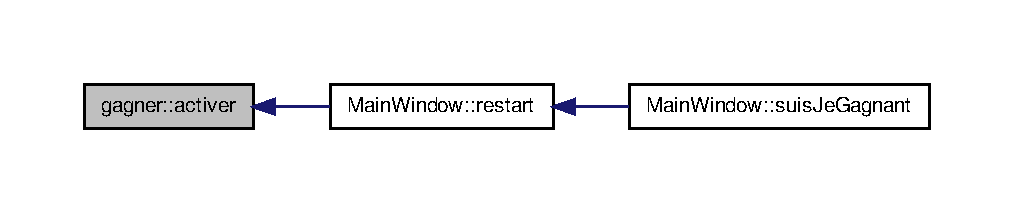
\includegraphics[width=350pt]{classgagner_ae397abfcf09f7e766e1661c99fa49a0c_icgraph}
\end{center}
\end{figure}


\hypertarget{classgagner_ace76d831ed95d4402be08bf9473081d3}{\index{gagner@{gagner}!on\-\_\-push\-Button\-Merci\-\_\-clicked@{on\-\_\-push\-Button\-Merci\-\_\-clicked}}
\index{on\-\_\-push\-Button\-Merci\-\_\-clicked@{on\-\_\-push\-Button\-Merci\-\_\-clicked}!gagner@{gagner}}
\subsubsection[{on\-\_\-push\-Button\-Merci\-\_\-clicked}]{\setlength{\rightskip}{0pt plus 5cm}void gagner\-::on\-\_\-push\-Button\-Merci\-\_\-clicked (
\begin{DoxyParamCaption}
{}
\end{DoxyParamCaption}
)\hspace{0.3cm}{\ttfamily [private]}, {\ttfamily [slot]}}}\label{classgagner_ace76d831ed95d4402be08bf9473081d3}


on\-\_\-push\-Button\-Merci\-\_\-clicked 



Définition à la ligne 31 du fichier gagner.\-cpp.



\subsection{Documentation des données membres}
\hypertarget{classgagner_a4b1df163878c34bff176f83bf01d1c26}{\index{gagner@{gagner}!ui@{ui}}
\index{ui@{ui}!gagner@{gagner}}
\subsubsection[{ui}]{\setlength{\rightskip}{0pt plus 5cm}Ui\-::gagner$\ast$ gagner\-::ui\hspace{0.3cm}{\ttfamily [private]}}}\label{classgagner_a4b1df163878c34bff176f83bf01d1c26}


ui 



Définition à la ligne 37 du fichier gagner.\-h.



La documentation de cette classe a été générée à partir des fichiers suivants \-:\begin{DoxyCompactItemize}
\item 
/home/arnaud/ptit\-Cailloux/\hyperlink{gagner_8h}{gagner.\-h}\item 
/home/arnaud/ptit\-Cailloux/\hyperlink{gagner_8cpp}{gagner.\-cpp}\end{DoxyCompactItemize}

\hypertarget{class_main_window_1_1h}{\section{Référence de la classe Main\-Window\-:\-:h}
\label{class_main_window_1_1h}\index{Main\-Window\-::h@{Main\-Window\-::h}}
}


This is the \hyperlink{class_main_window}{Main\-Window} class.  




{\ttfamily \#include $<$mainwindow.\-h$>$}



\subsection{Description détaillée}
This is the \hyperlink{class_main_window}{Main\-Window} class. 

La documentation de cette classe a été générée à partir du fichier suivant \-:\begin{DoxyCompactItemize}
\item 
/home/arnaud/ptit\-Cailloux/\hyperlink{mainwindow_8h}{mainwindow.\-h}\end{DoxyCompactItemize}

\hypertarget{interfaceorg_1_1kde_1_1necessitas_1_1ministro_1_1_i_ministro}{\section{Référence de l'interface org.\-kde.\-necessitas.\-ministro.\-I\-Ministro}
\label{interfaceorg_1_1kde_1_1necessitas_1_1ministro_1_1_i_ministro}\index{org.\-kde.\-necessitas.\-ministro.\-I\-Ministro@{org.\-kde.\-necessitas.\-ministro.\-I\-Ministro}}
}


Graphe d'héritage de org.\-kde.\-necessitas.\-ministro.\-I\-Ministro\-:\nopagebreak
\begin{figure}[H]
\begin{center}
\leavevmode
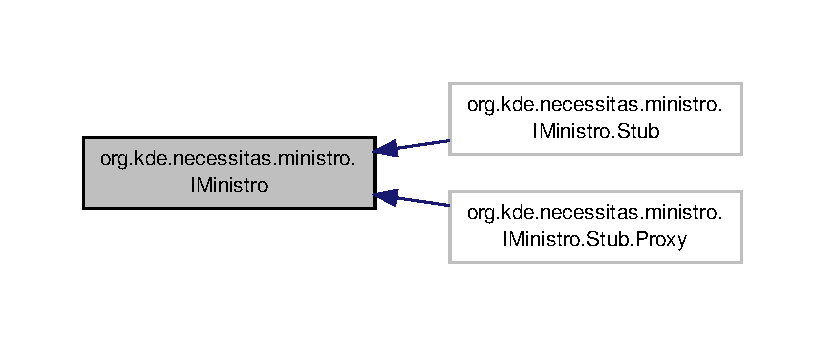
\includegraphics[width=350pt]{interfaceorg_1_1kde_1_1necessitas_1_1ministro_1_1_i_ministro__inherit__graph}
\end{center}
\end{figure}
\subsection*{Classes}
\begin{DoxyCompactItemize}
\item 
class {\bfseries Stub}
\end{DoxyCompactItemize}
\subsection*{Fonctions membres publiques}
\begin{DoxyCompactItemize}
\item 
void \hyperlink{interfaceorg_1_1kde_1_1necessitas_1_1ministro_1_1_i_ministro_a3d7c6602e2f6151d53df20f674b97af1}{request\-Loader} (\hyperlink{interfaceorg_1_1kde_1_1necessitas_1_1ministro_1_1_i_ministro_callback}{org.\-kde.\-necessitas.\-ministro.\-I\-Ministro\-Callback} callback, android.\-os.\-Bundle parameters)  throws android.\-os.\-Remote\-Exception
\end{DoxyCompactItemize}


\subsection{Description détaillée}


Définition à la ligne 6 du fichier I\-Ministro.\-java.



\subsection{Documentation des fonctions membres}
\hypertarget{interfaceorg_1_1kde_1_1necessitas_1_1ministro_1_1_i_ministro_a3d7c6602e2f6151d53df20f674b97af1}{\index{org\-::kde\-::necessitas\-::ministro\-::\-I\-Ministro@{org\-::kde\-::necessitas\-::ministro\-::\-I\-Ministro}!request\-Loader@{request\-Loader}}
\index{request\-Loader@{request\-Loader}!org::kde::necessitas::ministro::IMinistro@{org\-::kde\-::necessitas\-::ministro\-::\-I\-Ministro}}
\subsubsection[{request\-Loader}]{\setlength{\rightskip}{0pt plus 5cm}void org.\-kde.\-necessitas.\-ministro.\-I\-Ministro.\-request\-Loader (
\begin{DoxyParamCaption}
\item[{{\bf org.\-kde.\-necessitas.\-ministro.\-I\-Ministro\-Callback}}]{callback, }
\item[{android.\-os.\-Bundle}]{parameters}
\end{DoxyParamCaption}
)  throws android.\-os.\-Remote\-Exception}}\label{interfaceorg_1_1kde_1_1necessitas_1_1ministro_1_1_i_ministro_a3d7c6602e2f6151d53df20f674b97af1}
Check/download required libs to run the application

param callback -\/ interface used by Minsitro service to notify the client when the loader is ready param parameters parameters fields\-:
\begin{DoxyItemize}
\item Key Name Key type Explanations \char`\"{}sources\char`\"{} String\-Array Sources list from where Ministro will download the libs. Make sure you are using O\-N\-L\-Y secure locations. \char`\"{}repository\char`\"{} String Overwrites the default Ministro repository. Possible values\-: default, stable, testing and unstable \char`\"{}required.\-modules\char`\"{} String\-Array Required modules by your application \char`\"{}application.\-title\char`\"{} String Application name, used to show more informations to user \char`\"{}qt.\-provider\char`\"{} String Qt libs provider, currently only \char`\"{}necessitas\char`\"{} is supported. \char`\"{}minimum.\-ministro.\-api\char`\"{} Integer Minimum Ministro A\-P\-I level, used to check if Ministro service compatible with your application. Current A\-P\-I Level is 3 ! \char`\"{}minimum.\-qt.\-version\char`\"{} Integer Minimim Qt version (e.\-g. 0x040800, which means Qt 4.\-8.\-0, check \href{http://qt-project.org/doc/qt-4.8/qtglobal.html#QT_VERSION}{\tt http\-://qt-\/project.\-org/doc/qt-\/4.\-8/qtglobal.\-html\#\-Q\-T\-\_\-\-V\-E\-R\-S\-I\-O\-N})! 
\end{DoxyItemize}

La documentation de cette interface a été générée à partir du fichier suivant \-:\begin{DoxyCompactItemize}
\item 
/home/arnaud/ptit\-Cailloux/android/gen/org/kde/necessitas/ministro/\hyperlink{_i_ministro_8java}{I\-Ministro.\-java}\end{DoxyCompactItemize}

\hypertarget{interfaceorg_1_1kde_1_1necessitas_1_1ministro_1_1_i_ministro_callback}{\section{Référence de l'interface org.\-kde.\-necessitas.\-ministro.\-I\-Ministro\-Callback}
\label{interfaceorg_1_1kde_1_1necessitas_1_1ministro_1_1_i_ministro_callback}\index{org.\-kde.\-necessitas.\-ministro.\-I\-Ministro\-Callback@{org.\-kde.\-necessitas.\-ministro.\-I\-Ministro\-Callback}}
}


Graphe d'héritage de org.\-kde.\-necessitas.\-ministro.\-I\-Ministro\-Callback\-:\nopagebreak
\begin{figure}[H]
\begin{center}
\leavevmode
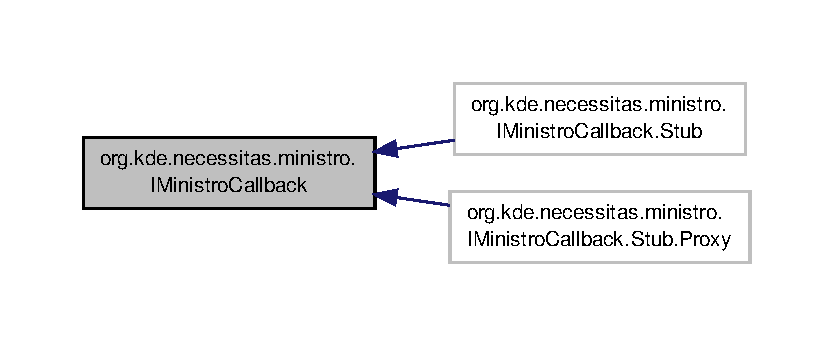
\includegraphics[width=350pt]{interfaceorg_1_1kde_1_1necessitas_1_1ministro_1_1_i_ministro_callback__inherit__graph}
\end{center}
\end{figure}
\subsection*{Classes}
\begin{DoxyCompactItemize}
\item 
class {\bfseries Stub}
\end{DoxyCompactItemize}
\subsection*{Fonctions membres publiques}
\begin{DoxyCompactItemize}
\item 
void \hyperlink{interfaceorg_1_1kde_1_1necessitas_1_1ministro_1_1_i_ministro_callback_ac67b08ed6184a57c5c732f2f8911a3bf}{loader\-Ready} (android.\-os.\-Bundle loader\-Params)  throws android.\-os.\-Remote\-Exception
\end{DoxyCompactItemize}


\subsection{Description détaillée}


Définition à la ligne 6 du fichier I\-Ministro\-Callback.\-java.



\subsection{Documentation des fonctions membres}
\hypertarget{interfaceorg_1_1kde_1_1necessitas_1_1ministro_1_1_i_ministro_callback_ac67b08ed6184a57c5c732f2f8911a3bf}{\index{org\-::kde\-::necessitas\-::ministro\-::\-I\-Ministro\-Callback@{org\-::kde\-::necessitas\-::ministro\-::\-I\-Ministro\-Callback}!loader\-Ready@{loader\-Ready}}
\index{loader\-Ready@{loader\-Ready}!org::kde::necessitas::ministro::IMinistroCallback@{org\-::kde\-::necessitas\-::ministro\-::\-I\-Ministro\-Callback}}
\subsubsection[{loader\-Ready}]{\setlength{\rightskip}{0pt plus 5cm}void org.\-kde.\-necessitas.\-ministro.\-I\-Ministro\-Callback.\-loader\-Ready (
\begin{DoxyParamCaption}
\item[{android.\-os.\-Bundle}]{loader\-Params}
\end{DoxyParamCaption}
)  throws android.\-os.\-Remote\-Exception}}\label{interfaceorg_1_1kde_1_1necessitas_1_1ministro_1_1_i_ministro_callback_ac67b08ed6184a57c5c732f2f8911a3bf}
This method is called by the Ministro service back into the application which implements this interface.

param in -\/ loader\-Params loader\-Params fields\-:
\begin{DoxyItemize}
\item Key Name Key type Explanations
\item \char`\"{}error.\-code\char`\"{} Integer See below
\item \char`\"{}error.\-message\char`\"{} String Missing if no error, otherwise will contain the error message translated into phone language where available.
\item \char`\"{}dex.\-path\char`\"{} String The list of jar/apk files containing classes and resources, needed to be passed to application Dex\-Class\-Loader
\item \char`\"{}lib.\-path\char`\"{} String The list of directories containing native libraries; may be missing, needed to be passed to application Dex\-Class\-Loader
\item \char`\"{}loader.\-class.\-name\char`\"{} String Loader class name.
\end{DoxyItemize}

\char`\"{}error.\-code\char`\"{} field possible errors\-:
\begin{DoxyItemize}
\item 0 no error.
\item 1 incompatible Ministro version. Ministro needs to be upgraded.
\item 2 not all modules could be satisfy.
\item 3 invalid parameters
\item 4 invalid qt version
\item 5 download canceled
\end{DoxyItemize}

The parameter contains additional fields which are used by the loader to start your application, so it must be passed to the loader. 

La documentation de cette interface a été générée à partir du fichier suivant \-:\begin{DoxyCompactItemize}
\item 
/home/arnaud/ptit\-Cailloux/android/gen/org/kde/necessitas/ministro/\hyperlink{_i_ministro_callback_8java}{I\-Ministro\-Callback.\-java}\end{DoxyCompactItemize}

\hypertarget{class_joueur}{\section{Référence de la classe Joueur}
\label{class_joueur}\index{Joueur@{Joueur}}
}


{\ttfamily \#include $<$joueur.\-h$>$}

\subsection*{Fonctions membres publiques}
\begin{DoxyCompactItemize}
\item 
\hyperlink{class_joueur_ae7289c7fcab027cba1299692f27c84b5}{Joueur} (Q\-Widget $\ast$parent=0)
\begin{DoxyCompactList}\small\item\em \hyperlink{class_joueur}{Joueur}. \end{DoxyCompactList}\item 
void \hyperlink{class_joueur_aca86d063fc2ab8c0733a17a508a41e36}{suis\-Je\-Gagnant} (int P1, int P2, int P3)
\begin{DoxyCompactList}\small\item\em suis\-Je\-Gagnant \end{DoxyCompactList}\end{DoxyCompactItemize}


\subsection{Description détaillée}


Définition à la ligne 5 du fichier joueur.\-h.



\subsection{Documentation des constructeurs et destructeur}
\hypertarget{class_joueur_ae7289c7fcab027cba1299692f27c84b5}{\index{Joueur@{Joueur}!Joueur@{Joueur}}
\index{Joueur@{Joueur}!Joueur@{Joueur}}
\subsubsection[{Joueur}]{\setlength{\rightskip}{0pt plus 5cm}Joueur\-::\-Joueur (
\begin{DoxyParamCaption}
\item[{Q\-Widget $\ast$}]{parent = {\ttfamily 0}}
\end{DoxyParamCaption}
)\hspace{0.3cm}{\ttfamily [explicit]}}}\label{class_joueur_ae7289c7fcab027cba1299692f27c84b5}


\hyperlink{class_joueur}{Joueur}. 


\begin{DoxyParams}{Paramètres}
{\em parent} & \\
\hline
\end{DoxyParams}


Définition à la ligne 7 du fichier joueur.\-cpp.



\subsection{Documentation des fonctions membres}
\hypertarget{class_joueur_aca86d063fc2ab8c0733a17a508a41e36}{\index{Joueur@{Joueur}!suis\-Je\-Gagnant@{suis\-Je\-Gagnant}}
\index{suis\-Je\-Gagnant@{suis\-Je\-Gagnant}!Joueur@{Joueur}}
\subsubsection[{suis\-Je\-Gagnant}]{\setlength{\rightskip}{0pt plus 5cm}void Joueur\-::suis\-Je\-Gagnant (
\begin{DoxyParamCaption}
\item[{int}]{P1, }
\item[{int}]{P2, }
\item[{int}]{P3}
\end{DoxyParamCaption}
)}}\label{class_joueur_aca86d063fc2ab8c0733a17a508a41e36}


suis\-Je\-Gagnant 


\begin{DoxyParams}{Paramètres}
{\em P1} & \\
\hline
{\em P2} & \\
\hline
{\em P3} & \\
\hline
\end{DoxyParams}


Définition à la ligne 11 du fichier joueur.\-cpp.



La documentation de cette classe a été générée à partir des fichiers suivants \-:\begin{DoxyCompactItemize}
\item 
/home/arnaud/ptit\-Cailloux/\hyperlink{joueur_8h}{joueur.\-h}\item 
/home/arnaud/ptit\-Cailloux/\hyperlink{joueur_8cpp}{joueur.\-cpp}\end{DoxyCompactItemize}

\hypertarget{class_main_window}{\section{Référence de la classe Main\-Window}
\label{class_main_window}\index{Main\-Window@{Main\-Window}}
}


{\ttfamily \#include $<$mainwindow.\-h$>$}

\subsection*{Classes}
\begin{DoxyCompactItemize}
\item 
class \hyperlink{class_main_window_1_1h}{h}
\begin{DoxyCompactList}\small\item\em This is the \hyperlink{class_main_window}{Main\-Window} class. \end{DoxyCompactList}\end{DoxyCompactItemize}
\subsection*{Fonctions membres publiques}
\begin{DoxyCompactItemize}
\item 
\hyperlink{class_main_window_a8b244be8b7b7db1b08de2a2acb9409db}{Main\-Window} (Q\-Widget $\ast$parent=0)
\begin{DoxyCompactList}\small\item\em \hyperlink{class_main_window}{Main\-Window}. \end{DoxyCompactList}\item 
void \hyperlink{class_main_window_a191288a043481fa695e4e546e2f76038}{nouveau\-Jeu} ()
\begin{DoxyCompactList}\small\item\em nouveau\-Jeu \end{DoxyCompactList}\item 
void \hyperlink{class_main_window_aded5036dd1d5ab1c06417b80ce705aef}{restart} (int joueur\-Gagnant)
\begin{DoxyCompactList}\small\item\em restart \end{DoxyCompactList}\item 
void \hyperlink{class_main_window_aee18876c586f3b6c1f668a040c9145cf}{suis\-Je\-Gagnant} (int P1, int P2, int P3)
\begin{DoxyCompactList}\small\item\em suis\-Je\-Gagnant \end{DoxyCompactList}\item 
\hyperlink{class_main_window_ae98d00a93bc118200eeef9f9bba1dba7}{$\sim$\-Main\-Window} ()
\end{DoxyCompactItemize}
\subsection*{Attributs publics}
\begin{DoxyCompactItemize}
\item 
double \hyperlink{class_main_window_a86efc7c173a08f153d7c781a9bb7dfe0}{coof\-X}
\begin{DoxyCompactList}\small\item\em coof\-X \end{DoxyCompactList}\item 
double \hyperlink{class_main_window_a2f2474d5ae1f34d4800e8fb67cf609af}{coof\-Y}
\begin{DoxyCompactList}\small\item\em coof\-Y \end{DoxyCompactList}\item 
bool \hyperlink{class_main_window_a7c53199a6fe3faad4ca98a78766a2863}{pos\-Ok}
\begin{DoxyCompactList}\small\item\em pos\-Ok \end{DoxyCompactList}\item 
int \hyperlink{class_main_window_a7b2b2add6bd8d72fb18f0f43c9998cb8}{tour\-Du\-Joueur} = 1
\begin{DoxyCompactList}\small\item\em donne le tour du joueur. \end{DoxyCompactList}\item 
bool \hyperlink{class_main_window_addef95af943f4874df6489bf08f2a516}{tous\-Sur\-Le\-Plateau}
\begin{DoxyCompactList}\small\item\em tous\-Sur\-Le\-Plateau \end{DoxyCompactList}\item 
int \hyperlink{class_main_window_a3356efaa3ec31594ed925406751cb1ab}{tout\-Placer} = 0
\begin{DoxyCompactList}\small\item\em tout\-Placer \end{DoxyCompactList}\item 
Ui\-::\-Main\-Window $\ast$ \hyperlink{class_main_window_a35466a70ed47252a0191168126a352a5}{ui}
\item 
Q\-Vector$<$ \hyperlink{classpion}{pion} $\ast$ $>$ \hyperlink{class_main_window_a972ef4345f96449207b78b25c170e0ba}{v\-Pion\-Pion}
\begin{DoxyCompactList}\small\item\em vecteur qui contient les pions. \end{DoxyCompactList}\item 
Q\-Vector$<$ Q\-Point $>$ \hyperlink{class_main_window_a8d561e817c4df106f2b54fe14d3e86f3}{v\-Pion\-Pos}
\begin{DoxyCompactList}\small\item\em vecteur qui contient les positions des pions sur le plateau \end{DoxyCompactList}\item 
Q\-Vector$<$ Q\-Point $>$ \hyperlink{class_main_window_a83813767ed28ca71358707f562095cf1}{v\-Pos}
\begin{DoxyCompactList}\small\item\em vecteur qui contient les positions possibles sur le plateau \end{DoxyCompactList}\item 
Q\-Vector$<$ bool $>$ \hyperlink{class_main_window_ad7397a5dbe03868a4b2502e0a993fcf4}{v\-Pos\-Libre}
\begin{DoxyCompactList}\small\item\em vecteur qui contient dit si la position est libre ou non. \end{DoxyCompactList}\end{DoxyCompactItemize}
\subsection*{Fonctions membres privées}
\begin{DoxyCompactItemize}
\item 
void \hyperlink{class_main_window_a5214e7f990954599ef57d8b08ee3eea0}{creer\-Pions} ()
\begin{DoxyCompactList}\small\item\em creer\-Pions \end{DoxyCompactList}\end{DoxyCompactItemize}


\subsection{Description détaillée}


Définition à la ligne 15 du fichier mainwindow.\-h.



\subsection{Documentation des constructeurs et destructeur}
\hypertarget{class_main_window_a8b244be8b7b7db1b08de2a2acb9409db}{\index{Main\-Window@{Main\-Window}!Main\-Window@{Main\-Window}}
\index{Main\-Window@{Main\-Window}!MainWindow@{Main\-Window}}
\subsubsection[{Main\-Window}]{\setlength{\rightskip}{0pt plus 5cm}Main\-Window\-::\-Main\-Window (
\begin{DoxyParamCaption}
\item[{Q\-Widget $\ast$}]{parent = {\ttfamily 0}}
\end{DoxyParamCaption}
)\hspace{0.3cm}{\ttfamily [explicit]}}}\label{class_main_window_a8b244be8b7b7db1b08de2a2acb9409db}


\hyperlink{class_main_window}{Main\-Window}. 


\begin{DoxyParams}{Paramètres}
{\em parent} & \\
\hline
\end{DoxyParams}
A\-N\-D\-R\-O\-I\-D

X\-X\-X 

Définition à la ligne 8 du fichier mainwindow.\-cpp.



Voici le graphe d'appel pour cette fonction \-:\nopagebreak
\begin{figure}[H]
\begin{center}
\leavevmode
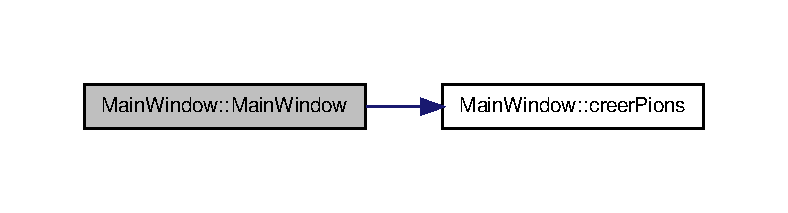
\includegraphics[width=350pt]{class_main_window_a8b244be8b7b7db1b08de2a2acb9409db_cgraph}
\end{center}
\end{figure}


\hypertarget{class_main_window_ae98d00a93bc118200eeef9f9bba1dba7}{\index{Main\-Window@{Main\-Window}!$\sim$\-Main\-Window@{$\sim$\-Main\-Window}}
\index{$\sim$\-Main\-Window@{$\sim$\-Main\-Window}!MainWindow@{Main\-Window}}
\subsubsection[{$\sim$\-Main\-Window}]{\setlength{\rightskip}{0pt plus 5cm}Main\-Window\-::$\sim$\-Main\-Window (
\begin{DoxyParamCaption}
{}
\end{DoxyParamCaption}
)}}\label{class_main_window_ae98d00a93bc118200eeef9f9bba1dba7}


Définition à la ligne 36 du fichier mainwindow.\-cpp.



\subsection{Documentation des fonctions membres}
\hypertarget{class_main_window_a5214e7f990954599ef57d8b08ee3eea0}{\index{Main\-Window@{Main\-Window}!creer\-Pions@{creer\-Pions}}
\index{creer\-Pions@{creer\-Pions}!MainWindow@{Main\-Window}}
\subsubsection[{creer\-Pions}]{\setlength{\rightskip}{0pt plus 5cm}void Main\-Window\-::creer\-Pions (
\begin{DoxyParamCaption}
{}
\end{DoxyParamCaption}
)\hspace{0.3cm}{\ttfamily [private]}}}\label{class_main_window_a5214e7f990954599ef57d8b08ee3eea0}


creer\-Pions 



Définition à la ligne 201 du fichier mainwindow.\-cpp.



Voici le graphe des appelants de cette fonction \-:\nopagebreak
\begin{figure}[H]
\begin{center}
\leavevmode
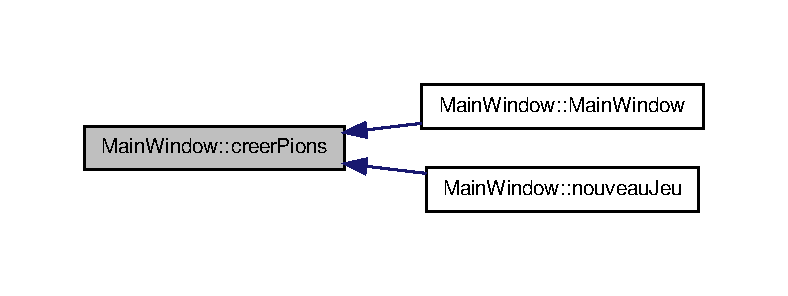
\includegraphics[width=350pt]{class_main_window_a5214e7f990954599ef57d8b08ee3eea0_icgraph}
\end{center}
\end{figure}


\hypertarget{class_main_window_a191288a043481fa695e4e546e2f76038}{\index{Main\-Window@{Main\-Window}!nouveau\-Jeu@{nouveau\-Jeu}}
\index{nouveau\-Jeu@{nouveau\-Jeu}!MainWindow@{Main\-Window}}
\subsubsection[{nouveau\-Jeu}]{\setlength{\rightskip}{0pt plus 5cm}void Main\-Window\-::nouveau\-Jeu (
\begin{DoxyParamCaption}
{}
\end{DoxyParamCaption}
)}}\label{class_main_window_a191288a043481fa695e4e546e2f76038}


nouveau\-Jeu 



Définition à la ligne 181 du fichier mainwindow.\-cpp.



Voici le graphe d'appel pour cette fonction \-:\nopagebreak
\begin{figure}[H]
\begin{center}
\leavevmode
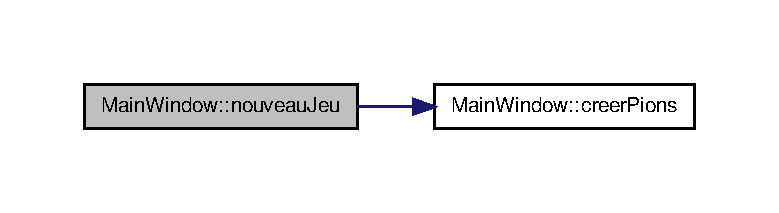
\includegraphics[width=350pt]{class_main_window_a191288a043481fa695e4e546e2f76038_cgraph}
\end{center}
\end{figure}


\hypertarget{class_main_window_aded5036dd1d5ab1c06417b80ce705aef}{\index{Main\-Window@{Main\-Window}!restart@{restart}}
\index{restart@{restart}!MainWindow@{Main\-Window}}
\subsubsection[{restart}]{\setlength{\rightskip}{0pt plus 5cm}void Main\-Window\-::restart (
\begin{DoxyParamCaption}
\item[{int}]{joueur\-Gagnant}
\end{DoxyParamCaption}
)}}\label{class_main_window_aded5036dd1d5ab1c06417b80ce705aef}


restart 


\begin{DoxyParams}{Paramètres}
{\em joueur\-Gagnant} & \\
\hline
\end{DoxyParams}


Définition à la ligne 173 du fichier mainwindow.\-cpp.



Voici le graphe d'appel pour cette fonction \-:\nopagebreak
\begin{figure}[H]
\begin{center}
\leavevmode
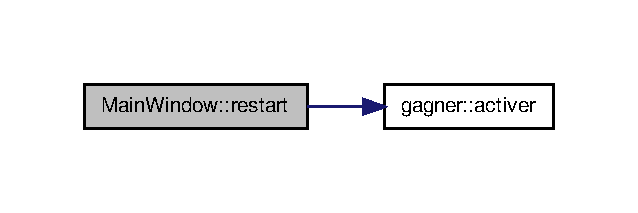
\includegraphics[width=306pt]{class_main_window_aded5036dd1d5ab1c06417b80ce705aef_cgraph}
\end{center}
\end{figure}




Voici le graphe des appelants de cette fonction \-:\nopagebreak
\begin{figure}[H]
\begin{center}
\leavevmode
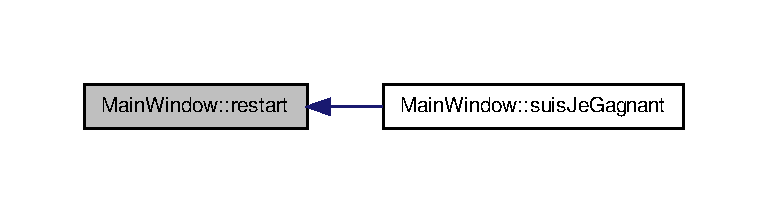
\includegraphics[width=350pt]{class_main_window_aded5036dd1d5ab1c06417b80ce705aef_icgraph}
\end{center}
\end{figure}


\hypertarget{class_main_window_aee18876c586f3b6c1f668a040c9145cf}{\index{Main\-Window@{Main\-Window}!suis\-Je\-Gagnant@{suis\-Je\-Gagnant}}
\index{suis\-Je\-Gagnant@{suis\-Je\-Gagnant}!MainWindow@{Main\-Window}}
\subsubsection[{suis\-Je\-Gagnant}]{\setlength{\rightskip}{0pt plus 5cm}void Main\-Window\-::suis\-Je\-Gagnant (
\begin{DoxyParamCaption}
\item[{int}]{P1, }
\item[{int}]{P2, }
\item[{int}]{P3}
\end{DoxyParamCaption}
)}}\label{class_main_window_aee18876c586f3b6c1f668a040c9145cf}


suis\-Je\-Gagnant 


\begin{DoxyParams}{Paramètres}
{\em P1} & \\
\hline
{\em P2} & \\
\hline
{\em P3} & \\
\hline
\end{DoxyParams}


Définition à la ligne 41 du fichier mainwindow.\-cpp.



Voici le graphe d'appel pour cette fonction \-:\nopagebreak
\begin{figure}[H]
\begin{center}
\leavevmode
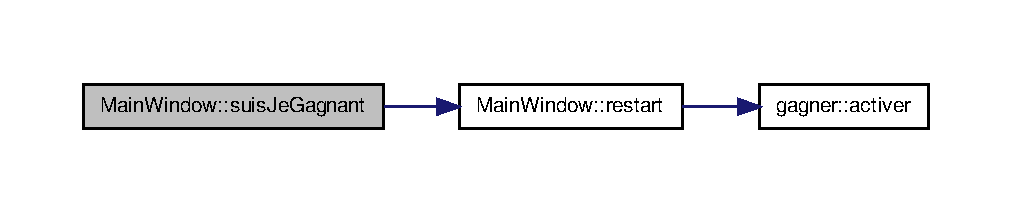
\includegraphics[width=350pt]{class_main_window_aee18876c586f3b6c1f668a040c9145cf_cgraph}
\end{center}
\end{figure}




\subsection{Documentation des données membres}
\hypertarget{class_main_window_a86efc7c173a08f153d7c781a9bb7dfe0}{\index{Main\-Window@{Main\-Window}!coof\-X@{coof\-X}}
\index{coof\-X@{coof\-X}!MainWindow@{Main\-Window}}
\subsubsection[{coof\-X}]{\setlength{\rightskip}{0pt plus 5cm}double Main\-Window\-::coof\-X}}\label{class_main_window_a86efc7c173a08f153d7c781a9bb7dfe0}


coof\-X 



Définition à la ligne 82 du fichier mainwindow.\-h.

\hypertarget{class_main_window_a2f2474d5ae1f34d4800e8fb67cf609af}{\index{Main\-Window@{Main\-Window}!coof\-Y@{coof\-Y}}
\index{coof\-Y@{coof\-Y}!MainWindow@{Main\-Window}}
\subsubsection[{coof\-Y}]{\setlength{\rightskip}{0pt plus 5cm}double Main\-Window\-::coof\-Y}}\label{class_main_window_a2f2474d5ae1f34d4800e8fb67cf609af}


coof\-Y 



Définition à la ligne 87 du fichier mainwindow.\-h.

\hypertarget{class_main_window_a7c53199a6fe3faad4ca98a78766a2863}{\index{Main\-Window@{Main\-Window}!pos\-Ok@{pos\-Ok}}
\index{pos\-Ok@{pos\-Ok}!MainWindow@{Main\-Window}}
\subsubsection[{pos\-Ok}]{\setlength{\rightskip}{0pt plus 5cm}bool Main\-Window\-::pos\-Ok}}\label{class_main_window_a7c53199a6fe3faad4ca98a78766a2863}


pos\-Ok 



Définition à la ligne 67 du fichier mainwindow.\-h.

\hypertarget{class_main_window_a7b2b2add6bd8d72fb18f0f43c9998cb8}{\index{Main\-Window@{Main\-Window}!tour\-Du\-Joueur@{tour\-Du\-Joueur}}
\index{tour\-Du\-Joueur@{tour\-Du\-Joueur}!MainWindow@{Main\-Window}}
\subsubsection[{tour\-Du\-Joueur}]{\setlength{\rightskip}{0pt plus 5cm}int Main\-Window\-::tour\-Du\-Joueur = 1}}\label{class_main_window_a7b2b2add6bd8d72fb18f0f43c9998cb8}


donne le tour du joueur. 

\begin{DoxyReturn}{Renvoie}
le numéro du joueur.
\end{DoxyReturn}
variable contenant un entier correspondant au numéro du joueur dont c'est le tour. 

Définition à la ligne 62 du fichier mainwindow.\-h.

\hypertarget{class_main_window_addef95af943f4874df6489bf08f2a516}{\index{Main\-Window@{Main\-Window}!tous\-Sur\-Le\-Plateau@{tous\-Sur\-Le\-Plateau}}
\index{tous\-Sur\-Le\-Plateau@{tous\-Sur\-Le\-Plateau}!MainWindow@{Main\-Window}}
\subsubsection[{tous\-Sur\-Le\-Plateau}]{\setlength{\rightskip}{0pt plus 5cm}bool Main\-Window\-::tous\-Sur\-Le\-Plateau}}\label{class_main_window_addef95af943f4874df6489bf08f2a516}


tous\-Sur\-Le\-Plateau 



Définition à la ligne 77 du fichier mainwindow.\-h.

\hypertarget{class_main_window_a3356efaa3ec31594ed925406751cb1ab}{\index{Main\-Window@{Main\-Window}!tout\-Placer@{tout\-Placer}}
\index{tout\-Placer@{tout\-Placer}!MainWindow@{Main\-Window}}
\subsubsection[{tout\-Placer}]{\setlength{\rightskip}{0pt plus 5cm}int Main\-Window\-::tout\-Placer = 0}}\label{class_main_window_a3356efaa3ec31594ed925406751cb1ab}


tout\-Placer 



Définition à la ligne 72 du fichier mainwindow.\-h.

\hypertarget{class_main_window_a35466a70ed47252a0191168126a352a5}{\index{Main\-Window@{Main\-Window}!ui@{ui}}
\index{ui@{ui}!MainWindow@{Main\-Window}}
\subsubsection[{ui}]{\setlength{\rightskip}{0pt plus 5cm}Ui\-::\-Main\-Window$\ast$ Main\-Window\-::ui}}\label{class_main_window_a35466a70ed47252a0191168126a352a5}


Définition à la ligne 29 du fichier mainwindow.\-h.

\hypertarget{class_main_window_a972ef4345f96449207b78b25c170e0ba}{\index{Main\-Window@{Main\-Window}!v\-Pion\-Pion@{v\-Pion\-Pion}}
\index{v\-Pion\-Pion@{v\-Pion\-Pion}!MainWindow@{Main\-Window}}
\subsubsection[{v\-Pion\-Pion}]{\setlength{\rightskip}{0pt plus 5cm}Q\-Vector$<${\bf pion}$\ast$$>$ Main\-Window\-::v\-Pion\-Pion}}\label{class_main_window_a972ef4345f96449207b78b25c170e0ba}


vecteur qui contient les pions. 



Définition à la ligne 53 du fichier mainwindow.\-h.

\hypertarget{class_main_window_a8d561e817c4df106f2b54fe14d3e86f3}{\index{Main\-Window@{Main\-Window}!v\-Pion\-Pos@{v\-Pion\-Pos}}
\index{v\-Pion\-Pos@{v\-Pion\-Pos}!MainWindow@{Main\-Window}}
\subsubsection[{v\-Pion\-Pos}]{\setlength{\rightskip}{0pt plus 5cm}Q\-Vector$<$Q\-Point$>$ Main\-Window\-::v\-Pion\-Pos}}\label{class_main_window_a8d561e817c4df106f2b54fe14d3e86f3}


vecteur qui contient les positions des pions sur le plateau 



Définition à la ligne 40 du fichier mainwindow.\-h.

\hypertarget{class_main_window_a83813767ed28ca71358707f562095cf1}{\index{Main\-Window@{Main\-Window}!v\-Pos@{v\-Pos}}
\index{v\-Pos@{v\-Pos}!MainWindow@{Main\-Window}}
\subsubsection[{v\-Pos}]{\setlength{\rightskip}{0pt plus 5cm}Q\-Vector$<$Q\-Point$>$ Main\-Window\-::v\-Pos}}\label{class_main_window_a83813767ed28ca71358707f562095cf1}


vecteur qui contient les positions possibles sur le plateau 



Définition à la ligne 34 du fichier mainwindow.\-h.

\hypertarget{class_main_window_ad7397a5dbe03868a4b2502e0a993fcf4}{\index{Main\-Window@{Main\-Window}!v\-Pos\-Libre@{v\-Pos\-Libre}}
\index{v\-Pos\-Libre@{v\-Pos\-Libre}!MainWindow@{Main\-Window}}
\subsubsection[{v\-Pos\-Libre}]{\setlength{\rightskip}{0pt plus 5cm}Q\-Vector$<$bool$>$ Main\-Window\-::v\-Pos\-Libre}}\label{class_main_window_ad7397a5dbe03868a4b2502e0a993fcf4}


vecteur qui contient dit si la position est libre ou non. 

\begin{DoxyReturn}{Renvoie}
vrai si il n'y a pas de pions sur la position et faux si elle est occupé. 
\end{DoxyReturn}


Définition à la ligne 48 du fichier mainwindow.\-h.



La documentation de cette classe a été générée à partir des fichiers suivants \-:\begin{DoxyCompactItemize}
\item 
/home/arnaud/ptit\-Cailloux/\hyperlink{mainwindow_8h}{mainwindow.\-h}\item 
/home/arnaud/ptit\-Cailloux/\hyperlink{mainwindow_8cpp}{mainwindow.\-cpp}\end{DoxyCompactItemize}

\hypertarget{classpion}{\section{Référence de la classe pion}
\label{classpion}\index{pion@{pion}}
}


{\ttfamily \#include $<$pion.\-h$>$}

\subsection*{Fonctions membres publiques}
\begin{DoxyCompactItemize}
\item 
\hyperlink{classpion_af29e3925ea85d612aea7e659254f401b}{pion} (Q\-Widget $\ast$parent=0, int no\-Pion=0, int x=50, int y=50)
\begin{DoxyCompactList}\small\item\em pion \end{DoxyCompactList}\end{DoxyCompactItemize}
\subsection*{Fonctions membres privées}
\begin{DoxyCompactItemize}
\item 
void \hyperlink{classpion_a14da0a4cb182706ced199d4f8d61dcd9}{droits} (int indice)
\begin{DoxyCompactList}\small\item\em droits \end{DoxyCompactList}\item 
void \hyperlink{classpion_a28e0a7d35ac53067f27a00152f221b60}{mouse\-Move\-Event} (Q\-Mouse\-Event $\ast$ev)
\begin{DoxyCompactList}\small\item\em mouse\-Move\-Event \end{DoxyCompactList}\item 
void \hyperlink{classpion_a44680c9f0758100216aaf61f696f8cc5}{mouse\-Press\-Event} (Q\-Mouse\-Event $\ast$ev)
\begin{DoxyCompactList}\small\item\em mouse\-Press\-Event \end{DoxyCompactList}\item 
void \hyperlink{classpion_a3d85aab7adc10d4a9cb7326c7a5e3466}{mouse\-Release\-Event} (Q\-Mouse\-Event $\ast$ev)
\begin{DoxyCompactList}\small\item\em mouse\-Release\-Event \end{DoxyCompactList}\end{DoxyCompactItemize}
\subsection*{Attributs privés}
\begin{DoxyCompactItemize}
\item 
bool \hyperlink{classpion_a99fe9f6343fa8261506fb5140ffd7dfa}{a\-Le\-Droit}
\begin{DoxyCompactList}\small\item\em a\-Le\-Droit \end{DoxyCompactList}\item 
Q\-Point \hyperlink{classpion_a7642cd4d43560d2fd90c33aa566d2526}{bon\-Point}
\begin{DoxyCompactList}\small\item\em bon\-Point \end{DoxyCompactList}\item 
int \hyperlink{classpion_a432598bfa12510f56629bb8e4e44a6d1}{h} = 40
\begin{DoxyCompactList}\small\item\em h \end{DoxyCompactList}\item 
int \hyperlink{classpion_ac953cdf61df0ff4b445b278e3be2bffc}{old\-X}
\begin{DoxyCompactList}\small\item\em old\-X \end{DoxyCompactList}\item 
int \hyperlink{classpion_a842a7ce1b21307287e434dd9d598eaee}{old\-Y}
\begin{DoxyCompactList}\small\item\em old\-Y \end{DoxyCompactList}\item 
int \hyperlink{classpion_a7338c5dde99c3d415665776d76c2d2db}{pion\-Num}
\begin{DoxyCompactList}\small\item\em pion\-Num \end{DoxyCompactList}\item 
int \hyperlink{classpion_ada2a7530bcff33b54aeb9b082a8d7bdb}{w} = 35
\begin{DoxyCompactList}\small\item\em w \end{DoxyCompactList}\end{DoxyCompactItemize}


\subsection{Description détaillée}


Définition à la ligne 5 du fichier pion.\-h.



\subsection{Documentation des constructeurs et destructeur}
\hypertarget{classpion_af29e3925ea85d612aea7e659254f401b}{\index{pion@{pion}!pion@{pion}}
\index{pion@{pion}!pion@{pion}}
\subsubsection[{pion}]{\setlength{\rightskip}{0pt plus 5cm}pion\-::pion (
\begin{DoxyParamCaption}
\item[{Q\-Widget $\ast$}]{parent = {\ttfamily 0}, }
\item[{int}]{no\-Pion = {\ttfamily 0}, }
\item[{int}]{x = {\ttfamily 50}, }
\item[{int}]{y = {\ttfamily 50}}
\end{DoxyParamCaption}
)\hspace{0.3cm}{\ttfamily [explicit]}}}\label{classpion_af29e3925ea85d612aea7e659254f401b}


pion 


\begin{DoxyParams}{Paramètres}
{\em parent} & \\
\hline
{\em no\-Pion} & \\
\hline
{\em x} & \\
\hline
{\em y} & \\
\hline
\end{DoxyParams}


Définition à la ligne 8 du fichier pion.\-cpp.



\subsection{Documentation des fonctions membres}
\hypertarget{classpion_a14da0a4cb182706ced199d4f8d61dcd9}{\index{pion@{pion}!droits@{droits}}
\index{droits@{droits}!pion@{pion}}
\subsubsection[{droits}]{\setlength{\rightskip}{0pt plus 5cm}void pion\-::droits (
\begin{DoxyParamCaption}
\item[{int}]{indice}
\end{DoxyParamCaption}
)\hspace{0.3cm}{\ttfamily [private]}}}\label{classpion_a14da0a4cb182706ced199d4f8d61dcd9}


droits 


\begin{DoxyParams}{Paramètres}
{\em indice} & \\
\hline
\end{DoxyParams}


Définition à la ligne 210 du fichier pion.\-cpp.



Voici le graphe des appelants de cette fonction \-:\nopagebreak
\begin{figure}[H]
\begin{center}
\leavevmode
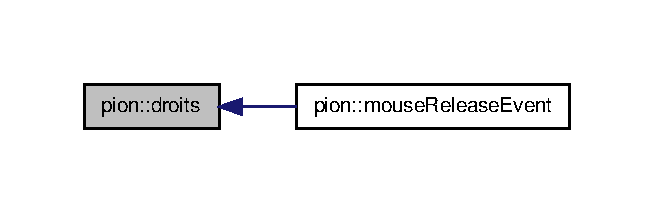
\includegraphics[width=314pt]{classpion_a14da0a4cb182706ced199d4f8d61dcd9_icgraph}
\end{center}
\end{figure}


\hypertarget{classpion_a28e0a7d35ac53067f27a00152f221b60}{\index{pion@{pion}!mouse\-Move\-Event@{mouse\-Move\-Event}}
\index{mouse\-Move\-Event@{mouse\-Move\-Event}!pion@{pion}}
\subsubsection[{mouse\-Move\-Event}]{\setlength{\rightskip}{0pt plus 5cm}void pion\-::mouse\-Move\-Event (
\begin{DoxyParamCaption}
\item[{Q\-Mouse\-Event $\ast$}]{ev}
\end{DoxyParamCaption}
)\hspace{0.3cm}{\ttfamily [private]}}}\label{classpion_a28e0a7d35ac53067f27a00152f221b60}


mouse\-Move\-Event 


\begin{DoxyParams}{Paramètres}
{\em ev} & \\
\hline
\end{DoxyParams}


Définition à la ligne 39 du fichier pion.\-cpp.

\hypertarget{classpion_a44680c9f0758100216aaf61f696f8cc5}{\index{pion@{pion}!mouse\-Press\-Event@{mouse\-Press\-Event}}
\index{mouse\-Press\-Event@{mouse\-Press\-Event}!pion@{pion}}
\subsubsection[{mouse\-Press\-Event}]{\setlength{\rightskip}{0pt plus 5cm}void pion\-::mouse\-Press\-Event (
\begin{DoxyParamCaption}
\item[{Q\-Mouse\-Event $\ast$}]{ev}
\end{DoxyParamCaption}
)\hspace{0.3cm}{\ttfamily [private]}}}\label{classpion_a44680c9f0758100216aaf61f696f8cc5}


mouse\-Press\-Event 


\begin{DoxyParams}{Paramètres}
{\em ev} & \\
\hline
\end{DoxyParams}


Définition à la ligne 30 du fichier pion.\-cpp.

\hypertarget{classpion_a3d85aab7adc10d4a9cb7326c7a5e3466}{\index{pion@{pion}!mouse\-Release\-Event@{mouse\-Release\-Event}}
\index{mouse\-Release\-Event@{mouse\-Release\-Event}!pion@{pion}}
\subsubsection[{mouse\-Release\-Event}]{\setlength{\rightskip}{0pt plus 5cm}void pion\-::mouse\-Release\-Event (
\begin{DoxyParamCaption}
\item[{Q\-Mouse\-Event $\ast$}]{ev}
\end{DoxyParamCaption}
)\hspace{0.3cm}{\ttfamily [private]}}}\label{classpion_a3d85aab7adc10d4a9cb7326c7a5e3466}


mouse\-Release\-Event 


\begin{DoxyParams}{Paramètres}
{\em ev} & \\
\hline
\end{DoxyParams}
X\-X\-X 

Définition à la ligne 100 du fichier pion.\-cpp.



Voici le graphe d'appel pour cette fonction \-:\nopagebreak
\begin{figure}[H]
\begin{center}
\leavevmode
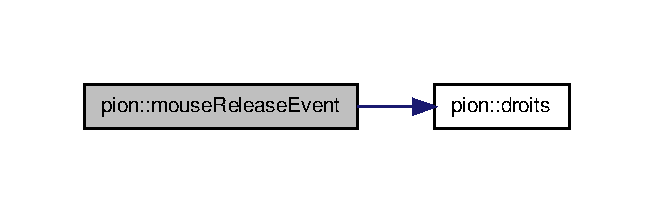
\includegraphics[width=314pt]{classpion_a3d85aab7adc10d4a9cb7326c7a5e3466_cgraph}
\end{center}
\end{figure}




\subsection{Documentation des données membres}
\hypertarget{classpion_a99fe9f6343fa8261506fb5140ffd7dfa}{\index{pion@{pion}!a\-Le\-Droit@{a\-Le\-Droit}}
\index{a\-Le\-Droit@{a\-Le\-Droit}!pion@{pion}}
\subsubsection[{a\-Le\-Droit}]{\setlength{\rightskip}{0pt plus 5cm}bool pion\-::a\-Le\-Droit\hspace{0.3cm}{\ttfamily [private]}}}\label{classpion_a99fe9f6343fa8261506fb5140ffd7dfa}


a\-Le\-Droit 



Définition à la ligne 62 du fichier pion.\-h.

\hypertarget{classpion_a7642cd4d43560d2fd90c33aa566d2526}{\index{pion@{pion}!bon\-Point@{bon\-Point}}
\index{bon\-Point@{bon\-Point}!pion@{pion}}
\subsubsection[{bon\-Point}]{\setlength{\rightskip}{0pt plus 5cm}Q\-Point pion\-::bon\-Point\hspace{0.3cm}{\ttfamily [private]}}}\label{classpion_a7642cd4d43560d2fd90c33aa566d2526}


bon\-Point 



Définition à la ligne 53 du fichier pion.\-h.

\hypertarget{classpion_a432598bfa12510f56629bb8e4e44a6d1}{\index{pion@{pion}!h@{h}}
\index{h@{h}!pion@{pion}}
\subsubsection[{h}]{\setlength{\rightskip}{0pt plus 5cm}int pion\-::h = 40\hspace{0.3cm}{\ttfamily [private]}}}\label{classpion_a432598bfa12510f56629bb8e4e44a6d1}


h 



Définition à la ligne 70 du fichier pion.\-h.

\hypertarget{classpion_ac953cdf61df0ff4b445b278e3be2bffc}{\index{pion@{pion}!old\-X@{old\-X}}
\index{old\-X@{old\-X}!pion@{pion}}
\subsubsection[{old\-X}]{\setlength{\rightskip}{0pt plus 5cm}int pion\-::old\-X\hspace{0.3cm}{\ttfamily [private]}}}\label{classpion_ac953cdf61df0ff4b445b278e3be2bffc}


old\-X 



Définition à la ligne 41 du fichier pion.\-h.

\hypertarget{classpion_a842a7ce1b21307287e434dd9d598eaee}{\index{pion@{pion}!old\-Y@{old\-Y}}
\index{old\-Y@{old\-Y}!pion@{pion}}
\subsubsection[{old\-Y}]{\setlength{\rightskip}{0pt plus 5cm}int pion\-::old\-Y\hspace{0.3cm}{\ttfamily [private]}}}\label{classpion_a842a7ce1b21307287e434dd9d598eaee}


old\-Y 



Définition à la ligne 45 du fichier pion.\-h.

\hypertarget{classpion_a7338c5dde99c3d415665776d76c2d2db}{\index{pion@{pion}!pion\-Num@{pion\-Num}}
\index{pion\-Num@{pion\-Num}!pion@{pion}}
\subsubsection[{pion\-Num}]{\setlength{\rightskip}{0pt plus 5cm}int pion\-::pion\-Num\hspace{0.3cm}{\ttfamily [private]}}}\label{classpion_a7338c5dde99c3d415665776d76c2d2db}


pion\-Num 



Définition à la ligne 49 du fichier pion.\-h.

\hypertarget{classpion_ada2a7530bcff33b54aeb9b082a8d7bdb}{\index{pion@{pion}!w@{w}}
\index{w@{w}!pion@{pion}}
\subsubsection[{w}]{\setlength{\rightskip}{0pt plus 5cm}int pion\-::w = 35\hspace{0.3cm}{\ttfamily [private]}}}\label{classpion_ada2a7530bcff33b54aeb9b082a8d7bdb}


w 



Définition à la ligne 66 du fichier pion.\-h.



La documentation de cette classe a été générée à partir des fichiers suivants \-:\begin{DoxyCompactItemize}
\item 
/home/arnaud/ptit\-Cailloux/\hyperlink{pion_8h}{pion.\-h}\item 
/home/arnaud/ptit\-Cailloux/\hyperlink{pion_8cpp}{pion.\-cpp}\end{DoxyCompactItemize}

\hypertarget{classorg_1_1qtproject_1_1qt5_1_1android_1_1bindings_1_1_qt_activity}{\section{Référence de la classe org.\-qtproject.\-qt5.\-android.\-bindings.\-Qt\-Activity}
\label{classorg_1_1qtproject_1_1qt5_1_1android_1_1bindings_1_1_qt_activity}\index{org.\-qtproject.\-qt5.\-android.\-bindings.\-Qt\-Activity@{org.\-qtproject.\-qt5.\-android.\-bindings.\-Qt\-Activity}}
}


Graphe d'héritage de org.\-qtproject.\-qt5.\-android.\-bindings.\-Qt\-Activity\-:\nopagebreak
\begin{figure}[H]
\begin{center}
\leavevmode
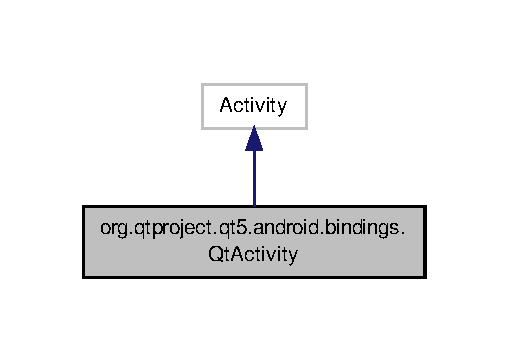
\includegraphics[width=244pt]{classorg_1_1qtproject_1_1qt5_1_1android_1_1bindings_1_1_qt_activity__inherit__graph}
\end{center}
\end{figure}


Graphe de collaboration de org.\-qtproject.\-qt5.\-android.\-bindings.\-Qt\-Activity\-:\nopagebreak
\begin{figure}[H]
\begin{center}
\leavevmode
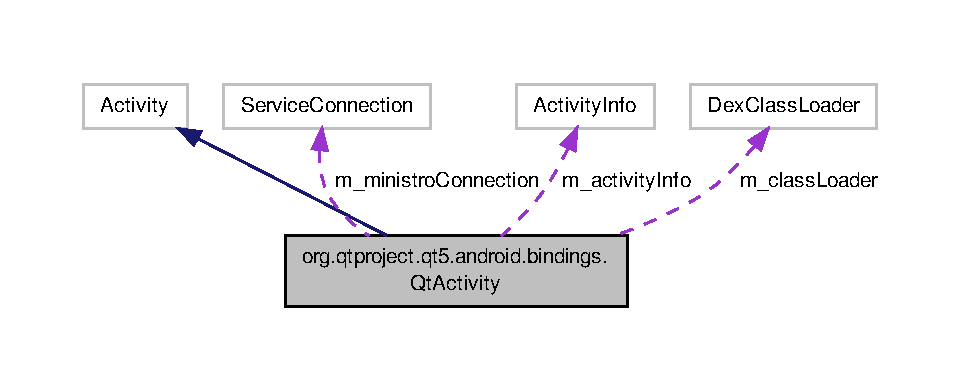
\includegraphics[width=350pt]{classorg_1_1qtproject_1_1qt5_1_1android_1_1bindings_1_1_qt_activity__coll__graph}
\end{center}
\end{figure}
\subsection*{Fonctions membres publiques}
\begin{DoxyCompactItemize}
\item 
boolean \hyperlink{classorg_1_1qtproject_1_1qt5_1_1android_1_1bindings_1_1_qt_activity_a3419f10b60670ae0fd0a222fcd684273}{dispatch\-Key\-Event} (Key\-Event event)
\item 
boolean \hyperlink{classorg_1_1qtproject_1_1qt5_1_1android_1_1bindings_1_1_qt_activity_a7eacf9d228567bace814d7d90cc88dc1}{dispatch\-Populate\-Accessibility\-Event} (Accessibility\-Event event)
\item 
boolean \hyperlink{classorg_1_1qtproject_1_1qt5_1_1android_1_1bindings_1_1_qt_activity_a080d702cac33de4a97b4645567cf8c04}{dispatch\-Touch\-Event} (Motion\-Event ev)
\item 
boolean \hyperlink{classorg_1_1qtproject_1_1qt5_1_1android_1_1bindings_1_1_qt_activity_ad305b6d78907e6fc4bc4fa9b77256a22}{dispatch\-Trackball\-Event} (Motion\-Event ev)
\item 
void \hyperlink{classorg_1_1qtproject_1_1qt5_1_1android_1_1bindings_1_1_qt_activity_a052fd4aee0de52bcf2d8a10c5671d586}{on\-Attached\-To\-Window} ()
\item 
void \hyperlink{classorg_1_1qtproject_1_1qt5_1_1android_1_1bindings_1_1_qt_activity_a593eeb49762865051c6348a6b98e7ff1}{on\-Back\-Pressed} ()
\item 
void \hyperlink{classorg_1_1qtproject_1_1qt5_1_1android_1_1bindings_1_1_qt_activity_a75ef70261caa7d4db3041147dc46c5d0}{on\-Configuration\-Changed} (Configuration new\-Config)
\item 
void \hyperlink{classorg_1_1qtproject_1_1qt5_1_1android_1_1bindings_1_1_qt_activity_a6310ffd404267a66b52dd4c3b357b560}{on\-Content\-Changed} ()
\item 
boolean \hyperlink{classorg_1_1qtproject_1_1qt5_1_1android_1_1bindings_1_1_qt_activity_a67108692da62e48e5d02b22ed3d83769}{on\-Context\-Item\-Selected} (Menu\-Item item)
\item 
void \hyperlink{classorg_1_1qtproject_1_1qt5_1_1android_1_1bindings_1_1_qt_activity_a3e845800dc8fc21ff23589005d1a781c}{on\-Context\-Menu\-Closed} (Menu menu)
\item 
void \hyperlink{classorg_1_1qtproject_1_1qt5_1_1android_1_1bindings_1_1_qt_activity_aa826639406d6f0697e0f1afcf69c748c}{on\-Create} (Bundle saved\-Instance\-State)
\item 
void \hyperlink{classorg_1_1qtproject_1_1qt5_1_1android_1_1bindings_1_1_qt_activity_a924489f96650a755cf63980f3d388e8e}{on\-Create\-Context\-Menu} (Context\-Menu menu, View v, Context\-Menu\-Info menu\-Info)
\item 
Char\-Sequence \hyperlink{classorg_1_1qtproject_1_1qt5_1_1android_1_1bindings_1_1_qt_activity_af86865337837c2c780913132b7118d69}{on\-Create\-Description} ()
\item 
boolean \hyperlink{classorg_1_1qtproject_1_1qt5_1_1android_1_1bindings_1_1_qt_activity_a9303a2dd16e8deb7cdcf143ae6b480f4}{on\-Create\-Options\-Menu} (Menu menu)
\item 
boolean \hyperlink{classorg_1_1qtproject_1_1qt5_1_1android_1_1bindings_1_1_qt_activity_a617b7c2c432bc9894d3c0b2490d27b41}{on\-Create\-Panel\-Menu} (int feature\-Id, Menu menu)
\item 
View \hyperlink{classorg_1_1qtproject_1_1qt5_1_1android_1_1bindings_1_1_qt_activity_aefde1977c2ccae37e5f1a927f7e9e9ee}{on\-Create\-Panel\-View} (int feature\-Id)
\item 
boolean \hyperlink{classorg_1_1qtproject_1_1qt5_1_1android_1_1bindings_1_1_qt_activity_a961e15fb9b7bcdc7e4310e881656e1d7}{on\-Create\-Thumbnail} (Bitmap out\-Bitmap, Canvas canvas)
\item 
View \hyperlink{classorg_1_1qtproject_1_1qt5_1_1android_1_1bindings_1_1_qt_activity_a4f26e1f33245742068eb9b79689f69e5}{on\-Create\-View} (String name, Context context, Attribute\-Set attrs)
\item 
void \hyperlink{classorg_1_1qtproject_1_1qt5_1_1android_1_1bindings_1_1_qt_activity_aa7cad0cee8c325c1cbd7bb77a8a2c5ce}{on\-Detached\-From\-Window} ()
\item 
boolean \hyperlink{classorg_1_1qtproject_1_1qt5_1_1android_1_1bindings_1_1_qt_activity_ac1ee5a8d6b1ed5e7757139be8d7810be}{on\-Key\-Down} (int key\-Code, Key\-Event event)
\item 
boolean \hyperlink{classorg_1_1qtproject_1_1qt5_1_1android_1_1bindings_1_1_qt_activity_ad1c024d3096ee30566b083bf35b711f4}{on\-Key\-Long\-Press} (int key\-Code, Key\-Event event)
\item 
boolean \hyperlink{classorg_1_1qtproject_1_1qt5_1_1android_1_1bindings_1_1_qt_activity_a9b41df58aada132667b9af5a8aa01aa7}{on\-Key\-Multiple} (int key\-Code, int repeat\-Count, Key\-Event event)
\item 
boolean \hyperlink{classorg_1_1qtproject_1_1qt5_1_1android_1_1bindings_1_1_qt_activity_ac81bcf0a973ed2f8035bc3af8ee73f78}{on\-Key\-Up} (int key\-Code, Key\-Event event)
\item 
void \hyperlink{classorg_1_1qtproject_1_1qt5_1_1android_1_1bindings_1_1_qt_activity_a60dde1c5c76102c0514119fbc9515450}{on\-Low\-Memory} ()
\item 
boolean \hyperlink{classorg_1_1qtproject_1_1qt5_1_1android_1_1bindings_1_1_qt_activity_a15f3f492aba46975a36f1ebdfbe5ba45}{on\-Menu\-Item\-Selected} (int feature\-Id, Menu\-Item item)
\item 
boolean \hyperlink{classorg_1_1qtproject_1_1qt5_1_1android_1_1bindings_1_1_qt_activity_afa718d6a5777a519b1d513d7cbda938a}{on\-Menu\-Opened} (int feature\-Id, Menu menu)
\item 
boolean \hyperlink{classorg_1_1qtproject_1_1qt5_1_1android_1_1bindings_1_1_qt_activity_a1062f0dfba41ba945835041b94bfe4fa}{on\-Options\-Item\-Selected} (Menu\-Item item)
\item 
void \hyperlink{classorg_1_1qtproject_1_1qt5_1_1android_1_1bindings_1_1_qt_activity_aad115f4cdaebb71916b85ac6309a83c4}{on\-Options\-Menu\-Closed} (Menu menu)
\item 
void \hyperlink{classorg_1_1qtproject_1_1qt5_1_1android_1_1bindings_1_1_qt_activity_a2b39eac5b8b7003b20171ddce6b16e37}{on\-Panel\-Closed} (int feature\-Id, Menu menu)
\item 
boolean \hyperlink{classorg_1_1qtproject_1_1qt5_1_1android_1_1bindings_1_1_qt_activity_a71a7e747de798c51b6a385b5e8a99c61}{on\-Prepare\-Options\-Menu} (Menu menu)
\item 
boolean \hyperlink{classorg_1_1qtproject_1_1qt5_1_1android_1_1bindings_1_1_qt_activity_a668c15554849a0bce9422eb709b5cacc}{on\-Prepare\-Panel} (int feature\-Id, View view, Menu menu)
\item 
Object \hyperlink{classorg_1_1qtproject_1_1qt5_1_1android_1_1bindings_1_1_qt_activity_a5954d45f88dd09deba757e671de9077d}{on\-Retain\-Non\-Configuration\-Instance} ()
\item 
boolean \hyperlink{classorg_1_1qtproject_1_1qt5_1_1android_1_1bindings_1_1_qt_activity_aa1c033b0b0bbc4cb9c193b239992fcb8}{on\-Search\-Requested} ()
\item 
boolean \hyperlink{classorg_1_1qtproject_1_1qt5_1_1android_1_1bindings_1_1_qt_activity_ada200302a153c7dbab3e55b746a7a179}{on\-Touch\-Event} (Motion\-Event event)
\item 
boolean \hyperlink{classorg_1_1qtproject_1_1qt5_1_1android_1_1bindings_1_1_qt_activity_a27faf58c38193faea2782ff85cedb567}{on\-Trackball\-Event} (Motion\-Event event)
\item 
void \hyperlink{classorg_1_1qtproject_1_1qt5_1_1android_1_1bindings_1_1_qt_activity_a3917d7d3ac6ab5bf31444d31b2784828}{on\-User\-Interaction} ()
\item 
void \hyperlink{classorg_1_1qtproject_1_1qt5_1_1android_1_1bindings_1_1_qt_activity_af881fa829fb552af632f8b1bba96f351}{on\-Window\-Attributes\-Changed} (Layout\-Params params)
\item 
void \hyperlink{classorg_1_1qtproject_1_1qt5_1_1android_1_1bindings_1_1_qt_activity_ab161d356ebf5044a00182ffaf79d3437}{on\-Window\-Focus\-Changed} (boolean has\-Focus)
\item 
boolean \hyperlink{classorg_1_1qtproject_1_1qt5_1_1android_1_1bindings_1_1_qt_activity_a0222dd1edd412d5573914d8e563d8dfc}{super\-\_\-dispatch\-Key\-Event} (Key\-Event event)
\item 
boolean \hyperlink{classorg_1_1qtproject_1_1qt5_1_1android_1_1bindings_1_1_qt_activity_a174082c8c4aa301a2a8c78ce237bca22}{super\-\_\-dispatch\-Populate\-Accessibility\-Event} (Accessibility\-Event event)
\item 
boolean \hyperlink{classorg_1_1qtproject_1_1qt5_1_1android_1_1bindings_1_1_qt_activity_a8525630fd66e1d88e94f7bc9457bbd1b}{super\-\_\-dispatch\-Touch\-Event} (Motion\-Event event)
\item 
boolean \hyperlink{classorg_1_1qtproject_1_1qt5_1_1android_1_1bindings_1_1_qt_activity_a84a82b3eb7dd352d126c55272c64264a}{super\-\_\-dispatch\-Trackball\-Event} (Motion\-Event event)
\item 
void \hyperlink{classorg_1_1qtproject_1_1qt5_1_1android_1_1bindings_1_1_qt_activity_a03bf6f3f50c07592cbee97ce9ebdb315}{super\-\_\-on\-Activity\-Result} (int request\-Code, int result\-Code, Intent data)
\item 
void \hyperlink{classorg_1_1qtproject_1_1qt5_1_1android_1_1bindings_1_1_qt_activity_a03b4db053b9528617c37bab2d47fc803}{super\-\_\-on\-Apply\-Theme\-Resource} (Theme theme, int resid, boolean first)
\item 
void \hyperlink{classorg_1_1qtproject_1_1qt5_1_1android_1_1bindings_1_1_qt_activity_a7155f32de8ac1f383e18250f28cd1f97}{super\-\_\-on\-Attached\-To\-Window} ()
\item 
void \hyperlink{classorg_1_1qtproject_1_1qt5_1_1android_1_1bindings_1_1_qt_activity_a84b318d75dea61b3aa2743fb475c90da}{super\-\_\-on\-Back\-Pressed} ()
\item 
void \hyperlink{classorg_1_1qtproject_1_1qt5_1_1android_1_1bindings_1_1_qt_activity_ac369eb38a2ea1f7a0d61c44a30d63620}{super\-\_\-on\-Child\-Title\-Changed} (Activity child\-Activity, Char\-Sequence title)
\item 
void \hyperlink{classorg_1_1qtproject_1_1qt5_1_1android_1_1bindings_1_1_qt_activity_a1c7f2e1b1ce16f2bfa70f38d88740565}{super\-\_\-on\-Configuration\-Changed} (Configuration new\-Config)
\item 
void \hyperlink{classorg_1_1qtproject_1_1qt5_1_1android_1_1bindings_1_1_qt_activity_a65dc57b70d42eb56f6bc12f7e0c49022}{super\-\_\-on\-Content\-Changed} ()
\item 
boolean \hyperlink{classorg_1_1qtproject_1_1qt5_1_1android_1_1bindings_1_1_qt_activity_a7281a498436213e739110753b357c0bd}{super\-\_\-on\-Context\-Item\-Selected} (Menu\-Item item)
\item 
void \hyperlink{classorg_1_1qtproject_1_1qt5_1_1android_1_1bindings_1_1_qt_activity_a1b845060cb1ae8dde9bb8a60339b9468}{super\-\_\-on\-Context\-Menu\-Closed} (Menu menu)
\item 
void \hyperlink{classorg_1_1qtproject_1_1qt5_1_1android_1_1bindings_1_1_qt_activity_ae235bff28fac3ae862e49a1fc52caf15}{super\-\_\-on\-Create\-Context\-Menu} (Context\-Menu menu, View v, Context\-Menu\-Info menu\-Info)
\item 
Char\-Sequence \hyperlink{classorg_1_1qtproject_1_1qt5_1_1android_1_1bindings_1_1_qt_activity_a213a5e7065a1b53244d8b3642a23b2e4}{super\-\_\-on\-Create\-Description} ()
\item 
Dialog \hyperlink{classorg_1_1qtproject_1_1qt5_1_1android_1_1bindings_1_1_qt_activity_a946099e0315e24f0c40338b69e0d1cdf}{super\-\_\-on\-Create\-Dialog} (int id)
\item 
Dialog \hyperlink{classorg_1_1qtproject_1_1qt5_1_1android_1_1bindings_1_1_qt_activity_a814d7e98bb1c0355ed33457de6718bee}{super\-\_\-on\-Create\-Dialog} (int id, Bundle args)
\item 
boolean \hyperlink{classorg_1_1qtproject_1_1qt5_1_1android_1_1bindings_1_1_qt_activity_a25d0cb2383a485b28f53026ebe050dd4}{super\-\_\-on\-Create\-Options\-Menu} (Menu menu)
\item 
boolean \hyperlink{classorg_1_1qtproject_1_1qt5_1_1android_1_1bindings_1_1_qt_activity_a3d105b186ba9bf7d089699dbd5ca3c45}{super\-\_\-on\-Create\-Panel\-Menu} (int feature\-Id, Menu menu)
\item 
View \hyperlink{classorg_1_1qtproject_1_1qt5_1_1android_1_1bindings_1_1_qt_activity_ab37f48e1ce50767f29be1cebd4fc96e0}{super\-\_\-on\-Create\-Panel\-View} (int feature\-Id)
\item 
boolean \hyperlink{classorg_1_1qtproject_1_1qt5_1_1android_1_1bindings_1_1_qt_activity_a2af36b766142fa45fa77623e549112ac}{super\-\_\-on\-Create\-Thumbnail} (Bitmap out\-Bitmap, Canvas canvas)
\item 
View \hyperlink{classorg_1_1qtproject_1_1qt5_1_1android_1_1bindings_1_1_qt_activity_a4e054eb047b9531cc8abaa75039136f2}{super\-\_\-on\-Create\-View} (String name, Context context, Attribute\-Set attrs)
\item 
void \hyperlink{classorg_1_1qtproject_1_1qt5_1_1android_1_1bindings_1_1_qt_activity_a103cd6d406de520a7c30fa31a704ee11}{super\-\_\-on\-Detached\-From\-Window} ()
\item 
boolean \hyperlink{classorg_1_1qtproject_1_1qt5_1_1android_1_1bindings_1_1_qt_activity_af7fbc3d78f28c7599fac81499717ac8d}{super\-\_\-on\-Key\-Down} (int key\-Code, Key\-Event event)
\item 
boolean \hyperlink{classorg_1_1qtproject_1_1qt5_1_1android_1_1bindings_1_1_qt_activity_ad723f98cf99880c9467f96f73fa25878}{super\-\_\-on\-Key\-Long\-Press} (int key\-Code, Key\-Event event)
\item 
boolean \hyperlink{classorg_1_1qtproject_1_1qt5_1_1android_1_1bindings_1_1_qt_activity_a108ba4840f9990f299beb44cced0a45d}{super\-\_\-on\-Key\-Multiple} (int key\-Code, int repeat\-Count, Key\-Event event)
\item 
boolean \hyperlink{classorg_1_1qtproject_1_1qt5_1_1android_1_1bindings_1_1_qt_activity_a0e236df83e1edd02ba8587199fc47e05}{super\-\_\-on\-Key\-Up} (int key\-Code, Key\-Event event)
\item 
boolean \hyperlink{classorg_1_1qtproject_1_1qt5_1_1android_1_1bindings_1_1_qt_activity_a054b8b51a53012f32a3d30bf395c18ca}{super\-\_\-on\-Menu\-Item\-Selected} (int feature\-Id, Menu\-Item item)
\item 
boolean \hyperlink{classorg_1_1qtproject_1_1qt5_1_1android_1_1bindings_1_1_qt_activity_ab1719c7260a5641289249620984077bd}{super\-\_\-on\-Menu\-Opened} (int feature\-Id, Menu menu)
\item 
void \hyperlink{classorg_1_1qtproject_1_1qt5_1_1android_1_1bindings_1_1_qt_activity_afb8a02b6c2e3c8e868f8cce113f50b18}{super\-\_\-on\-New\-Intent} (Intent intent)
\item 
boolean \hyperlink{classorg_1_1qtproject_1_1qt5_1_1android_1_1bindings_1_1_qt_activity_aab1ebb0d4fe4429af0b9e79a4a6295ad}{super\-\_\-on\-Options\-Item\-Selected} (Menu\-Item item)
\item 
void \hyperlink{classorg_1_1qtproject_1_1qt5_1_1android_1_1bindings_1_1_qt_activity_abd8ef4d5f57f3046c3065cbe806f690b}{super\-\_\-on\-Options\-Menu\-Closed} (Menu menu)
\item 
void \hyperlink{classorg_1_1qtproject_1_1qt5_1_1android_1_1bindings_1_1_qt_activity_a5f9ad8da2fcebff92ef8c86583091d75}{super\-\_\-on\-Panel\-Closed} (int feature\-Id, Menu menu)
\item 
void \hyperlink{classorg_1_1qtproject_1_1qt5_1_1android_1_1bindings_1_1_qt_activity_aacc652635f4bf45e2fa182dc44e8df13}{super\-\_\-on\-Prepare\-Dialog} (int id, Dialog dialog)
\item 
void \hyperlink{classorg_1_1qtproject_1_1qt5_1_1android_1_1bindings_1_1_qt_activity_a385e763c50fd7d00213fe961bba46ed5}{super\-\_\-on\-Prepare\-Dialog} (int id, Dialog dialog, Bundle args)
\item 
boolean \hyperlink{classorg_1_1qtproject_1_1qt5_1_1android_1_1bindings_1_1_qt_activity_a9f7f63be6b9a75253b784e80bfa74f69}{super\-\_\-on\-Prepare\-Options\-Menu} (Menu menu)
\item 
boolean \hyperlink{classorg_1_1qtproject_1_1qt5_1_1android_1_1bindings_1_1_qt_activity_ab8af6f3b5a5b4547829dc68e7c31fd86}{super\-\_\-on\-Prepare\-Panel} (int feature\-Id, View view, Menu menu)
\item 
void \hyperlink{classorg_1_1qtproject_1_1qt5_1_1android_1_1bindings_1_1_qt_activity_a73303f1db92072963fe8592eb05b0258}{super\-\_\-on\-Restore\-Instance\-State} (Bundle saved\-Instance\-State)
\item 
Object \hyperlink{classorg_1_1qtproject_1_1qt5_1_1android_1_1bindings_1_1_qt_activity_a4fa6ba75523273de5b492052f1ae06f0}{super\-\_\-on\-Retain\-Non\-Configuration\-Instance} ()
\item 
void \hyperlink{classorg_1_1qtproject_1_1qt5_1_1android_1_1bindings_1_1_qt_activity_a8fb26c42bd8d7516bf863cc5fb50e287}{super\-\_\-on\-Save\-Instance\-State} (Bundle out\-State)
\item 
boolean \hyperlink{classorg_1_1qtproject_1_1qt5_1_1android_1_1bindings_1_1_qt_activity_a41f90d68a12b8140f7b0f4c4037c2567}{super\-\_\-on\-Search\-Requested} ()
\item 
void \hyperlink{classorg_1_1qtproject_1_1qt5_1_1android_1_1bindings_1_1_qt_activity_aa3982942fa042ca69a13ffbaff0ef403}{super\-\_\-on\-Title\-Changed} (Char\-Sequence title, int color)
\item 
boolean \hyperlink{classorg_1_1qtproject_1_1qt5_1_1android_1_1bindings_1_1_qt_activity_a216ec445b2cc31beac2032e38dd5e949}{super\-\_\-on\-Touch\-Event} (Motion\-Event event)
\item 
boolean \hyperlink{classorg_1_1qtproject_1_1qt5_1_1android_1_1bindings_1_1_qt_activity_a4ee363f63dfde917e450b70c8880fef9}{super\-\_\-on\-Trackball\-Event} (Motion\-Event event)
\item 
void \hyperlink{classorg_1_1qtproject_1_1qt5_1_1android_1_1bindings_1_1_qt_activity_a706d78309b31669959a98b46952de75c}{super\-\_\-on\-User\-Interaction} ()
\item 
void \hyperlink{classorg_1_1qtproject_1_1qt5_1_1android_1_1bindings_1_1_qt_activity_ae71ad183d13c1bbb1fd1dccee12dde24}{super\-\_\-on\-User\-Leave\-Hint} ()
\item 
void \hyperlink{classorg_1_1qtproject_1_1qt5_1_1android_1_1bindings_1_1_qt_activity_aa510558df5227f66d81d6119389e7886}{super\-\_\-on\-Window\-Attributes\-Changed} (Layout\-Params params)
\item 
void \hyperlink{classorg_1_1qtproject_1_1qt5_1_1android_1_1bindings_1_1_qt_activity_a3d01ed848c426f937fe18214ff006931}{super\-\_\-on\-Window\-Focus\-Changed} (boolean has\-Focus)
\end{DoxyCompactItemize}
\subsection*{Fonctions membres protégées}
\begin{DoxyCompactItemize}
\item 
void \hyperlink{classorg_1_1qtproject_1_1qt5_1_1android_1_1bindings_1_1_qt_activity_a4e9a7c6b28384e4d5f713462207ffc41}{on\-Activity\-Result} (int request\-Code, int result\-Code, Intent data)
\item 
void \hyperlink{classorg_1_1qtproject_1_1qt5_1_1android_1_1bindings_1_1_qt_activity_acd279279e5ad448d802fa31b64a30aef}{on\-Apply\-Theme\-Resource} (Theme theme, int resid, boolean first)
\item 
void \hyperlink{classorg_1_1qtproject_1_1qt5_1_1android_1_1bindings_1_1_qt_activity_ac300f488c368a77573a3ecbf90f88b3c}{on\-Child\-Title\-Changed} (Activity child\-Activity, Char\-Sequence title)
\item 
Dialog \hyperlink{classorg_1_1qtproject_1_1qt5_1_1android_1_1bindings_1_1_qt_activity_a94b7cad79823109fd5ce75385766144b}{on\-Create\-Dialog} (int id)
\item 
Dialog \hyperlink{classorg_1_1qtproject_1_1qt5_1_1android_1_1bindings_1_1_qt_activity_a68654d4382feda0419fd1a59792b3643}{on\-Create\-Dialog} (int id, Bundle args)
\item 
void \hyperlink{classorg_1_1qtproject_1_1qt5_1_1android_1_1bindings_1_1_qt_activity_a30832553da49ca0dea222e062e21710c}{on\-Destroy} ()
\item 
void \hyperlink{classorg_1_1qtproject_1_1qt5_1_1android_1_1bindings_1_1_qt_activity_a995502b7cf803efcecc91d345b030404}{on\-New\-Intent} (Intent intent)
\item 
void \hyperlink{classorg_1_1qtproject_1_1qt5_1_1android_1_1bindings_1_1_qt_activity_a54af4563a2a1f3ea73187c2e9b9b042c}{on\-Pause} ()
\item 
void \hyperlink{classorg_1_1qtproject_1_1qt5_1_1android_1_1bindings_1_1_qt_activity_a1a206c815af224d5bf06e5c921f4fdd4}{on\-Post\-Create} (Bundle saved\-Instance\-State)
\item 
void \hyperlink{classorg_1_1qtproject_1_1qt5_1_1android_1_1bindings_1_1_qt_activity_af23189d66db86a4a4356af8481450fa1}{on\-Post\-Resume} ()
\item 
void \hyperlink{classorg_1_1qtproject_1_1qt5_1_1android_1_1bindings_1_1_qt_activity_a7c23883f7117af2b20250150e032935d}{on\-Prepare\-Dialog} (int id, Dialog dialog)
\item 
void \hyperlink{classorg_1_1qtproject_1_1qt5_1_1android_1_1bindings_1_1_qt_activity_aa4466dc136a61b68aaf83cf3a5a9827d}{on\-Prepare\-Dialog} (int id, Dialog dialog, Bundle args)
\item 
void \hyperlink{classorg_1_1qtproject_1_1qt5_1_1android_1_1bindings_1_1_qt_activity_a05a1cabee75d99161959de7575052b73}{on\-Restart} ()
\item 
void \hyperlink{classorg_1_1qtproject_1_1qt5_1_1android_1_1bindings_1_1_qt_activity_a0dd64ece074eb6909bb384a63105083b}{on\-Restore\-Instance\-State} (Bundle saved\-Instance\-State)
\item 
void \hyperlink{classorg_1_1qtproject_1_1qt5_1_1android_1_1bindings_1_1_qt_activity_a136a4d6d46f5a88c6e2b9866fa78fc64}{on\-Resume} ()
\item 
void \hyperlink{classorg_1_1qtproject_1_1qt5_1_1android_1_1bindings_1_1_qt_activity_ab32e70bfe633f137c58c82a96bf68f8f}{on\-Save\-Instance\-State} (Bundle out\-State)
\item 
void \hyperlink{classorg_1_1qtproject_1_1qt5_1_1android_1_1bindings_1_1_qt_activity_a5d86c0f23d31274741575dbf916814d1}{on\-Start} ()
\item 
void \hyperlink{classorg_1_1qtproject_1_1qt5_1_1android_1_1bindings_1_1_qt_activity_a2fa87ac6c9b33749654fb05211d7d894}{on\-Stop} ()
\item 
void \hyperlink{classorg_1_1qtproject_1_1qt5_1_1android_1_1bindings_1_1_qt_activity_ab084cdaffe2c7638d6c7e1255aecec3c}{on\-Title\-Changed} (Char\-Sequence title, int color)
\item 
void \hyperlink{classorg_1_1qtproject_1_1qt5_1_1android_1_1bindings_1_1_qt_activity_a86f980854e12f7cf5c8a91f7cbd875d7}{on\-User\-Leave\-Hint} ()
\end{DoxyCompactItemize}
\subsection*{Fonctions membres privées}
\begin{DoxyCompactItemize}
\item 
void \hyperlink{classorg_1_1qtproject_1_1qt5_1_1android_1_1bindings_1_1_qt_activity_a59050af1b747e4f7e5d68f5627ae94c9}{copy\-Asset} (String source, String destination)  throws I\-O\-Exception     
\item 
void \hyperlink{classorg_1_1qtproject_1_1qt5_1_1android_1_1bindings_1_1_qt_activity_abbade298e1a223acb5900e1ddd6ace74}{download\-Upgrade\-Ministro} (String msg)
\item 
void \hyperlink{classorg_1_1qtproject_1_1qt5_1_1android_1_1bindings_1_1_qt_activity_a38024ae043417efcc1b79aec389042b0}{extract\-Bundled\-Plugins\-And\-Imports} (String local\-Prefix)  throws I\-O\-Exception     
\item 
void \hyperlink{classorg_1_1qtproject_1_1qt5_1_1android_1_1bindings_1_1_qt_activity_aa72e2a52d4667eac2de67b9148c5332b}{load\-Application} (Bundle loader\-Params)
\item 
void \hyperlink{classorg_1_1qtproject_1_1qt5_1_1android_1_1bindings_1_1_qt_activity_a5e703f667905e2a0c11117197560d4e4}{ministro\-Not\-Found} ()
\item 
void \hyperlink{classorg_1_1qtproject_1_1qt5_1_1android_1_1bindings_1_1_qt_activity_a278365425c88a7b98bfcaf86b9a5a6ff}{start\-App} (final boolean first\-Start)
\end{DoxyCompactItemize}
\subsection*{Fonctions membres privées statiques}
\begin{DoxyCompactItemize}
\item 
static void \hyperlink{classorg_1_1qtproject_1_1qt5_1_1android_1_1bindings_1_1_qt_activity_a24e86e92cae2290e764995e64550f387}{copy\-File} (Input\-Stream input\-Stream, Output\-Stream output\-Stream)  throws I\-O\-Exception     
\item 
static void \hyperlink{classorg_1_1qtproject_1_1qt5_1_1android_1_1bindings_1_1_qt_activity_abfd0a80966d866beca1cfc2bc0b07b29}{create\-Bundled\-Binary} (String source, String destination)  throws I\-O\-Exception     
\end{DoxyCompactItemize}
\subsection*{Attributs privés}
\begin{DoxyCompactItemize}
\item 
Activity\-Info \hyperlink{classorg_1_1qtproject_1_1qt5_1_1android_1_1bindings_1_1_qt_activity_ab82e3c0917844afbd0559863f78137bf}{m\-\_\-activity\-Info} = null
\item 
Dex\-Class\-Loader \hyperlink{classorg_1_1qtproject_1_1qt5_1_1android_1_1bindings_1_1_qt_activity_a061ee56178d4d7ab6da01d7cf187e33b}{m\-\_\-class\-Loader} = null
\item 
Service\-Connection \hyperlink{classorg_1_1qtproject_1_1qt5_1_1android_1_1bindings_1_1_qt_activity_a26f7868b5d490d58265090a167e66436}{m\-\_\-ministro\-Connection}
\item 
String\mbox{[}$\,$\mbox{]} \hyperlink{classorg_1_1qtproject_1_1qt5_1_1android_1_1bindings_1_1_qt_activity_a18de4caf09f5386072f13afc426f2bce}{m\-\_\-qt\-Libs} = null
\item 
String \hyperlink{classorg_1_1qtproject_1_1qt5_1_1android_1_1bindings_1_1_qt_activity_a45d1a455c3855079063f6457a9dffb82}{m\-\_\-repository} = \char`\"{}default\char`\"{}
\item 
String\mbox{[}$\,$\mbox{]} \hyperlink{classorg_1_1qtproject_1_1qt5_1_1android_1_1bindings_1_1_qt_activity_a9cb36331162103703e5861eae9ce2caa}{m\-\_\-sources} = \{\char`\"{}https\-://download.\-qt-\/project.\-org/ministro/android/qt5/latest\char`\"{}\}
\end{DoxyCompactItemize}
\subsection*{Attributs privés statiques}
\begin{DoxyCompactItemize}
\item 
static final String \hyperlink{classorg_1_1qtproject_1_1qt5_1_1android_1_1bindings_1_1_qt_activity_a937cdab8f1ed3cd586583d88451925cd}{A\-P\-P\-L\-I\-C\-A\-T\-I\-O\-N\-\_\-\-P\-A\-R\-A\-M\-E\-T\-E\-R\-S} = null
\item 
static final String \hyperlink{classorg_1_1qtproject_1_1qt5_1_1android_1_1bindings_1_1_qt_activity_ae1f6a110a88016081007182f746540e9}{A\-P\-P\-L\-I\-C\-A\-T\-I\-O\-N\-\_\-\-P\-A\-R\-A\-M\-E\-T\-E\-R\-S\-\_\-\-K\-E\-Y} = \char`\"{}application.\-parameters\char`\"{}
\item 
static final String \hyperlink{classorg_1_1qtproject_1_1qt5_1_1android_1_1bindings_1_1_qt_activity_af4f23851df97539f4624239760dc422b}{A\-P\-P\-L\-I\-C\-A\-T\-I\-O\-N\-\_\-\-T\-I\-T\-L\-E\-\_\-\-K\-E\-Y} = \char`\"{}application.\-title\char`\"{}
\item 
static final int \hyperlink{classorg_1_1qtproject_1_1qt5_1_1android_1_1bindings_1_1_qt_activity_a837ce539bec41f495bfb09537e9080b5}{B\-U\-F\-F\-E\-R\-\_\-\-S\-I\-Z\-E} = 1024
\item 
static final String \hyperlink{classorg_1_1qtproject_1_1qt5_1_1android_1_1bindings_1_1_qt_activity_af1986a508d85b5d92de383c363423897}{B\-U\-N\-D\-L\-E\-D\-\_\-\-I\-N\-\_\-\-A\-S\-S\-E\-T\-S\-\_\-\-R\-E\-S\-O\-U\-R\-C\-E\-\_\-\-I\-D\-\_\-\-K\-E\-Y} = \char`\"{}android.\-app.\-bundled\-\_\-in\-\_\-assets\-\_\-resource\-\_\-id\char`\"{}
\item 
static final String \hyperlink{classorg_1_1qtproject_1_1qt5_1_1android_1_1bindings_1_1_qt_activity_ae43184b37ba175ea26b5993c2afae68b}{B\-U\-N\-D\-L\-E\-D\-\_\-\-I\-N\-\_\-\-L\-I\-B\-\_\-\-R\-E\-S\-O\-U\-R\-C\-E\-\_\-\-I\-D\-\_\-\-K\-E\-Y} = \char`\"{}android.\-app.\-bundled\-\_\-in\-\_\-lib\-\_\-resource\-\_\-id\char`\"{}
\item 
static final String \hyperlink{classorg_1_1qtproject_1_1qt5_1_1android_1_1bindings_1_1_qt_activity_adc2dfe1bdf822d0955cbaf2c881cf213}{B\-U\-N\-D\-L\-E\-D\-\_\-\-L\-I\-B\-R\-A\-R\-I\-E\-S\-\_\-\-K\-E\-Y} = \char`\"{}bundled.\-libraries\char`\"{}
\item 
static final String \hyperlink{classorg_1_1qtproject_1_1qt5_1_1android_1_1bindings_1_1_qt_activity_ae5aa0233d6c36a21c88e4e66dfe19c5b}{D\-E\-X\-\_\-\-P\-A\-T\-H\-\_\-\-K\-E\-Y} = \char`\"{}dex.\-path\char`\"{}
\item 
static final String \hyperlink{classorg_1_1qtproject_1_1qt5_1_1android_1_1bindings_1_1_qt_activity_ad15ba0bd0c50fec1a278b9e8df99a696}{E\-N\-V\-I\-R\-O\-N\-M\-E\-N\-T\-\_\-\-V\-A\-R\-I\-A\-B\-L\-E\-S} = \char`\"{}Q\-T\-\_\-\-U\-S\-E\-\_\-\-A\-N\-D\-R\-O\-I\-D\-\_\-\-N\-A\-T\-I\-V\-E\-\_\-\-S\-T\-Y\-L\-E=0\textbackslash{}t\char`\"{}
\item 
static final String \hyperlink{classorg_1_1qtproject_1_1qt5_1_1android_1_1bindings_1_1_qt_activity_a0ab4c9114f2c7fc3d558b434b94ca67d}{E\-N\-V\-I\-R\-O\-N\-M\-E\-N\-T\-\_\-\-V\-A\-R\-I\-A\-B\-L\-E\-S\-\_\-\-K\-E\-Y} = \char`\"{}environment.\-variables\char`\"{}
\item 
static final String \hyperlink{classorg_1_1qtproject_1_1qt5_1_1android_1_1bindings_1_1_qt_activity_a622fb5d7bef50ed00fffc6bbd2360471}{E\-R\-R\-O\-R\-\_\-\-C\-O\-D\-E\-\_\-\-K\-E\-Y} = \char`\"{}error.\-code\char`\"{}
\item 
static final String \hyperlink{classorg_1_1qtproject_1_1qt5_1_1android_1_1bindings_1_1_qt_activity_aca95fb0dcd299571b85b640343ed93cb}{E\-R\-R\-O\-R\-\_\-\-M\-E\-S\-S\-A\-G\-E\-\_\-\-K\-E\-Y} = \char`\"{}error.\-message\char`\"{}
\item 
static final int \hyperlink{classorg_1_1qtproject_1_1qt5_1_1android_1_1bindings_1_1_qt_activity_a5289c3884e015f388f7d02893cacc9e1}{I\-N\-C\-O\-M\-P\-A\-T\-I\-B\-L\-E\-\_\-\-M\-I\-N\-I\-S\-T\-R\-O\-\_\-\-V\-E\-R\-S\-I\-O\-N} = 1
\item 
static final String \hyperlink{classorg_1_1qtproject_1_1qt5_1_1android_1_1bindings_1_1_qt_activity_a5358dabbb2ba8b009dbe44c7edcc4456}{L\-I\-B\-\_\-\-P\-A\-T\-H\-\_\-\-K\-E\-Y} = \char`\"{}lib.\-path\char`\"{}
\item 
static final String \hyperlink{classorg_1_1qtproject_1_1qt5_1_1android_1_1bindings_1_1_qt_activity_addbda8603e3918a0c8cb3031e1629edd}{L\-O\-A\-D\-E\-R\-\_\-\-C\-L\-A\-S\-S\-\_\-\-N\-A\-M\-E\-\_\-\-K\-E\-Y} = \char`\"{}loader.\-class.\-name\char`\"{}
\item 
static final String \hyperlink{classorg_1_1qtproject_1_1qt5_1_1android_1_1bindings_1_1_qt_activity_a26a671584c763cc53820a168f2148705}{M\-A\-I\-N\-\_\-\-L\-I\-B\-R\-A\-R\-Y\-\_\-\-K\-E\-Y} = \char`\"{}main.\-library\char`\"{}
\item 
static final String \hyperlink{classorg_1_1qtproject_1_1qt5_1_1android_1_1bindings_1_1_qt_activity_ab771969e61a69b9ac3108af0e02a6037}{M\-I\-N\-I\-M\-U\-M\-\_\-\-M\-I\-N\-I\-S\-T\-R\-O\-\_\-\-A\-P\-I\-\_\-\-K\-E\-Y} = \char`\"{}minimum.\-ministro.\-api\char`\"{}
\item 
static final String \hyperlink{classorg_1_1qtproject_1_1qt5_1_1android_1_1bindings_1_1_qt_activity_a79571709091b556e9e51f663fdcbe480}{M\-I\-N\-I\-M\-U\-M\-\_\-\-Q\-T\-\_\-\-V\-E\-R\-S\-I\-O\-N\-\_\-\-K\-E\-Y} = \char`\"{}minimum.\-qt.\-version\char`\"{}
\item 
static final int \hyperlink{classorg_1_1qtproject_1_1qt5_1_1android_1_1bindings_1_1_qt_activity_a1d702f784aaa9626b73aff8afa7b0715}{M\-I\-N\-I\-S\-T\-R\-O\-\_\-\-A\-P\-I\-\_\-\-L\-E\-V\-E\-L} = 3
\item 
static final int \hyperlink{classorg_1_1qtproject_1_1qt5_1_1android_1_1bindings_1_1_qt_activity_a87a83049df392efc8f93ba4ca1370082}{M\-I\-N\-I\-S\-T\-R\-O\-\_\-\-I\-N\-S\-T\-A\-L\-L\-\_\-\-R\-E\-Q\-U\-E\-S\-T\-\_\-\-C\-O\-D\-E} = 0xf3ee
\item 
static final String \hyperlink{classorg_1_1qtproject_1_1qt5_1_1android_1_1bindings_1_1_qt_activity_aee09072d2bb95f2e30d5286a2d17b7df}{N\-A\-T\-I\-V\-E\-\_\-\-L\-I\-B\-R\-A\-R\-I\-E\-S\-\_\-\-K\-E\-Y} = \char`\"{}native.\-libraries\char`\"{}
\item 
static final int \hyperlink{classorg_1_1qtproject_1_1qt5_1_1android_1_1bindings_1_1_qt_activity_ae51d7ad4cace96487bb3bd69e3eecc1b}{N\-E\-C\-E\-S\-S\-I\-T\-A\-S\-\_\-\-A\-P\-I\-\_\-\-L\-E\-V\-E\-L} = 2
\item 
static final String \hyperlink{classorg_1_1qtproject_1_1qt5_1_1android_1_1bindings_1_1_qt_activity_a7c580751c3a85da7cffdaf1988e42fba}{N\-E\-C\-E\-S\-S\-I\-T\-A\-S\-\_\-\-A\-P\-I\-\_\-\-L\-E\-V\-E\-L\-\_\-\-K\-E\-Y} = \char`\"{}necessitas.\-api.\-level\char`\"{}
\item 
static final int \hyperlink{classorg_1_1qtproject_1_1qt5_1_1android_1_1bindings_1_1_qt_activity_a8671729726d87b492286bd3c774cb223}{Q\-T\-\_\-\-V\-E\-R\-S\-I\-O\-N} = 0x050100
\item 
static final String \hyperlink{classorg_1_1qtproject_1_1qt5_1_1android_1_1bindings_1_1_qt_activity_a183751882ba4d9384a7de07f3ec432ef}{R\-E\-P\-O\-S\-I\-T\-O\-R\-Y\-\_\-\-K\-E\-Y} = \char`\"{}repository\char`\"{}
\item 
static final String \hyperlink{classorg_1_1qtproject_1_1qt5_1_1android_1_1bindings_1_1_qt_activity_a1ce85e125b559f5f3dbc6e4e74be4f16}{R\-E\-Q\-U\-I\-R\-E\-D\-\_\-\-M\-O\-D\-U\-L\-E\-S\-\_\-\-K\-E\-Y} = \char`\"{}required.\-modules\char`\"{}
\begin{DoxyCompactList}\small\item\em Ministro server parameter keys. \end{DoxyCompactList}\item 
static final String \hyperlink{classorg_1_1qtproject_1_1qt5_1_1android_1_1bindings_1_1_qt_activity_a65f1863a6452fb6963ea25ffe511e203}{S\-O\-U\-R\-C\-E\-S\-\_\-\-K\-E\-Y} = \char`\"{}sources\char`\"{}
\item 
static final String \hyperlink{classorg_1_1qtproject_1_1qt5_1_1android_1_1bindings_1_1_qt_activity_a4378655de69dad520f1a678b6e972317}{S\-T\-A\-T\-I\-C\-\_\-\-I\-N\-I\-T\-\_\-\-C\-L\-A\-S\-S\-E\-S\-\_\-\-K\-E\-Y} = \char`\"{}static.\-init.\-classes\char`\"{}
\end{DoxyCompactItemize}


\subsection{Description détaillée}


Définition à la ligne 82 du fichier Qt\-Activity.\-java.



\subsection{Documentation des fonctions membres}
\hypertarget{classorg_1_1qtproject_1_1qt5_1_1android_1_1bindings_1_1_qt_activity_a59050af1b747e4f7e5d68f5627ae94c9}{\index{org\-::qtproject\-::qt5\-::android\-::bindings\-::\-Qt\-Activity@{org\-::qtproject\-::qt5\-::android\-::bindings\-::\-Qt\-Activity}!copy\-Asset@{copy\-Asset}}
\index{copy\-Asset@{copy\-Asset}!org::qtproject::qt5::android::bindings::QtActivity@{org\-::qtproject\-::qt5\-::android\-::bindings\-::\-Qt\-Activity}}
\subsubsection[{copy\-Asset}]{\setlength{\rightskip}{0pt plus 5cm}void org.\-qtproject.\-qt5.\-android.\-bindings.\-Qt\-Activity.\-copy\-Asset (
\begin{DoxyParamCaption}
\item[{String}]{source, }
\item[{String}]{destination}
\end{DoxyParamCaption}
)  throws I\-O\-Exception     \hspace{0.3cm}{\ttfamily [inline]}, {\ttfamily [private]}}}\label{classorg_1_1qtproject_1_1qt5_1_1android_1_1bindings_1_1_qt_activity_a59050af1b747e4f7e5d68f5627ae94c9}


Définition à la ligne 332 du fichier Qt\-Activity.\-java.



Voici le graphe d'appel pour cette fonction \-:\nopagebreak
\begin{figure}[H]
\begin{center}
\leavevmode
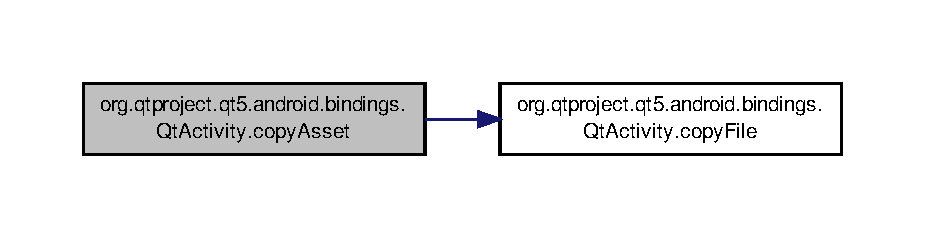
\includegraphics[width=350pt]{classorg_1_1qtproject_1_1qt5_1_1android_1_1bindings_1_1_qt_activity_a59050af1b747e4f7e5d68f5627ae94c9_cgraph}
\end{center}
\end{figure}




Voici le graphe des appelants de cette fonction \-:\nopagebreak
\begin{figure}[H]
\begin{center}
\leavevmode
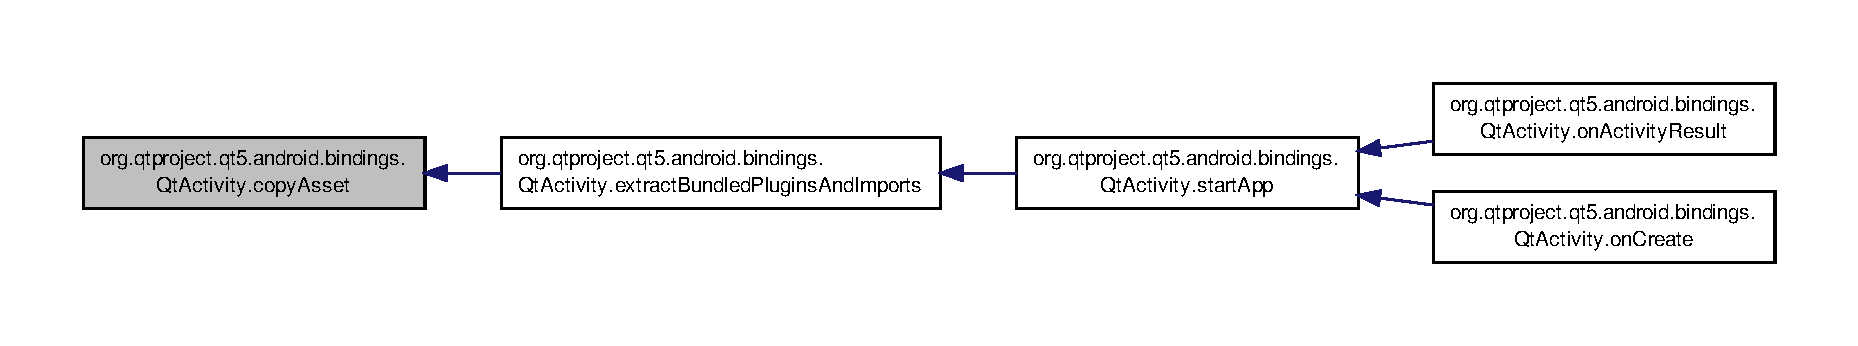
\includegraphics[width=350pt]{classorg_1_1qtproject_1_1qt5_1_1android_1_1bindings_1_1_qt_activity_a59050af1b747e4f7e5d68f5627ae94c9_icgraph}
\end{center}
\end{figure}


\hypertarget{classorg_1_1qtproject_1_1qt5_1_1android_1_1bindings_1_1_qt_activity_a24e86e92cae2290e764995e64550f387}{\index{org\-::qtproject\-::qt5\-::android\-::bindings\-::\-Qt\-Activity@{org\-::qtproject\-::qt5\-::android\-::bindings\-::\-Qt\-Activity}!copy\-File@{copy\-File}}
\index{copy\-File@{copy\-File}!org::qtproject::qt5::android::bindings::QtActivity@{org\-::qtproject\-::qt5\-::android\-::bindings\-::\-Qt\-Activity}}
\subsubsection[{copy\-File}]{\setlength{\rightskip}{0pt plus 5cm}static void org.\-qtproject.\-qt5.\-android.\-bindings.\-Qt\-Activity.\-copy\-File (
\begin{DoxyParamCaption}
\item[{Input\-Stream}]{input\-Stream, }
\item[{Output\-Stream}]{output\-Stream}
\end{DoxyParamCaption}
)  throws I\-O\-Exception     \hspace{0.3cm}{\ttfamily [inline]}, {\ttfamily [static]}, {\ttfamily [private]}}}\label{classorg_1_1qtproject_1_1qt5_1_1android_1_1bindings_1_1_qt_activity_a24e86e92cae2290e764995e64550f387}


Définition à la ligne 321 du fichier Qt\-Activity.\-java.



Voici le graphe des appelants de cette fonction \-:\nopagebreak
\begin{figure}[H]
\begin{center}
\leavevmode
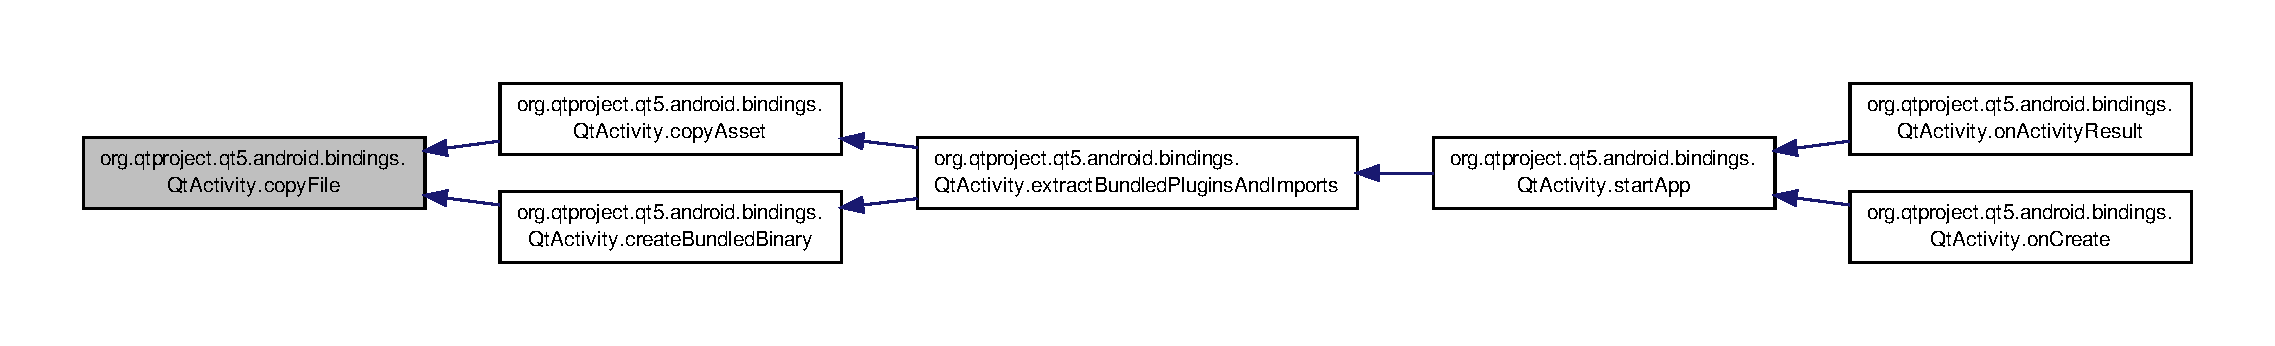
\includegraphics[width=350pt]{classorg_1_1qtproject_1_1qt5_1_1android_1_1bindings_1_1_qt_activity_a24e86e92cae2290e764995e64550f387_icgraph}
\end{center}
\end{figure}


\hypertarget{classorg_1_1qtproject_1_1qt5_1_1android_1_1bindings_1_1_qt_activity_abfd0a80966d866beca1cfc2bc0b07b29}{\index{org\-::qtproject\-::qt5\-::android\-::bindings\-::\-Qt\-Activity@{org\-::qtproject\-::qt5\-::android\-::bindings\-::\-Qt\-Activity}!create\-Bundled\-Binary@{create\-Bundled\-Binary}}
\index{create\-Bundled\-Binary@{create\-Bundled\-Binary}!org::qtproject::qt5::android::bindings::QtActivity@{org\-::qtproject\-::qt5\-::android\-::bindings\-::\-Qt\-Activity}}
\subsubsection[{create\-Bundled\-Binary}]{\setlength{\rightskip}{0pt plus 5cm}static void org.\-qtproject.\-qt5.\-android.\-bindings.\-Qt\-Activity.\-create\-Bundled\-Binary (
\begin{DoxyParamCaption}
\item[{String}]{source, }
\item[{String}]{destination}
\end{DoxyParamCaption}
)  throws I\-O\-Exception     \hspace{0.3cm}{\ttfamily [inline]}, {\ttfamily [static]}, {\ttfamily [private]}}}\label{classorg_1_1qtproject_1_1qt5_1_1android_1_1bindings_1_1_qt_activity_abfd0a80966d866beca1cfc2bc0b07b29}


Définition à la ligne 352 du fichier Qt\-Activity.\-java.



Voici le graphe d'appel pour cette fonction \-:\nopagebreak
\begin{figure}[H]
\begin{center}
\leavevmode
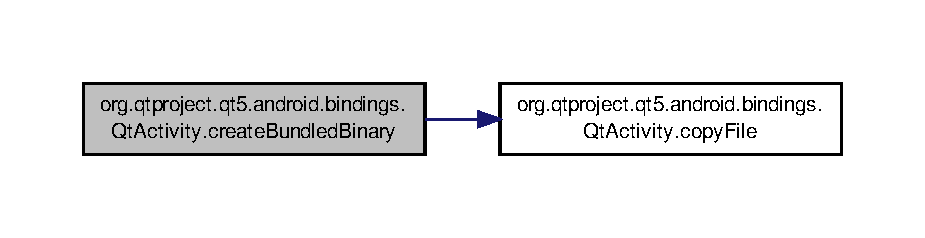
\includegraphics[width=350pt]{classorg_1_1qtproject_1_1qt5_1_1android_1_1bindings_1_1_qt_activity_abfd0a80966d866beca1cfc2bc0b07b29_cgraph}
\end{center}
\end{figure}




Voici le graphe des appelants de cette fonction \-:\nopagebreak
\begin{figure}[H]
\begin{center}
\leavevmode
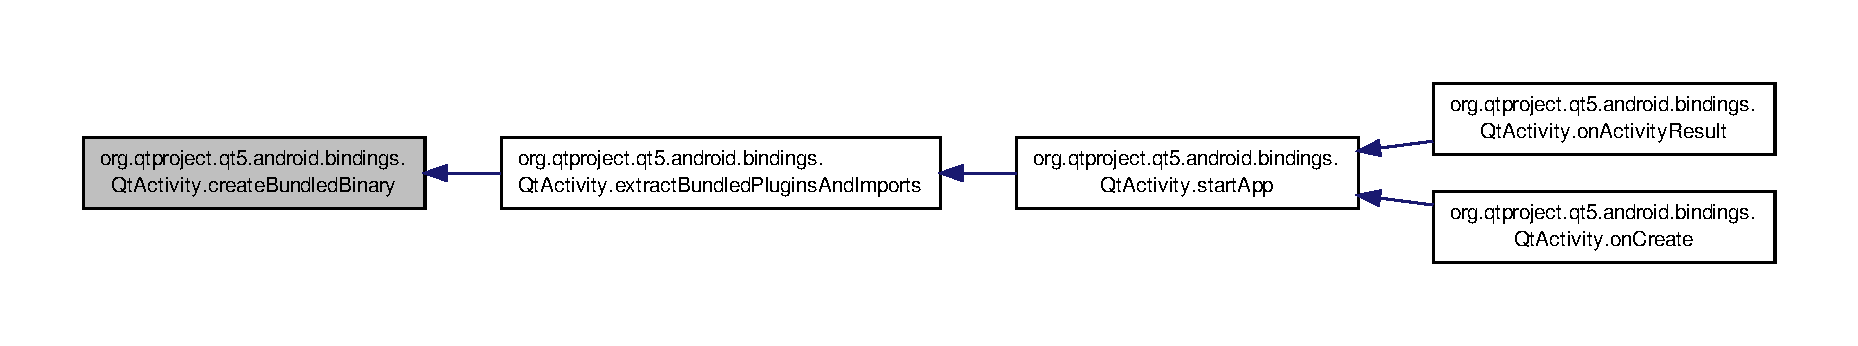
\includegraphics[width=350pt]{classorg_1_1qtproject_1_1qt5_1_1android_1_1bindings_1_1_qt_activity_abfd0a80966d866beca1cfc2bc0b07b29_icgraph}
\end{center}
\end{figure}


\hypertarget{classorg_1_1qtproject_1_1qt5_1_1android_1_1bindings_1_1_qt_activity_a3419f10b60670ae0fd0a222fcd684273}{\index{org\-::qtproject\-::qt5\-::android\-::bindings\-::\-Qt\-Activity@{org\-::qtproject\-::qt5\-::android\-::bindings\-::\-Qt\-Activity}!dispatch\-Key\-Event@{dispatch\-Key\-Event}}
\index{dispatch\-Key\-Event@{dispatch\-Key\-Event}!org::qtproject::qt5::android::bindings::QtActivity@{org\-::qtproject\-::qt5\-::android\-::bindings\-::\-Qt\-Activity}}
\subsubsection[{dispatch\-Key\-Event}]{\setlength{\rightskip}{0pt plus 5cm}boolean org.\-qtproject.\-qt5.\-android.\-bindings.\-Qt\-Activity.\-dispatch\-Key\-Event (
\begin{DoxyParamCaption}
\item[{Key\-Event}]{event}
\end{DoxyParamCaption}
)\hspace{0.3cm}{\ttfamily [inline]}}}\label{classorg_1_1qtproject_1_1qt5_1_1android_1_1bindings_1_1_qt_activity_a3419f10b60670ae0fd0a222fcd684273}


Définition à la ligne 517 du fichier Qt\-Activity.\-java.



Voici le graphe d'appel pour cette fonction \-:\nopagebreak
\begin{figure}[H]
\begin{center}
\leavevmode
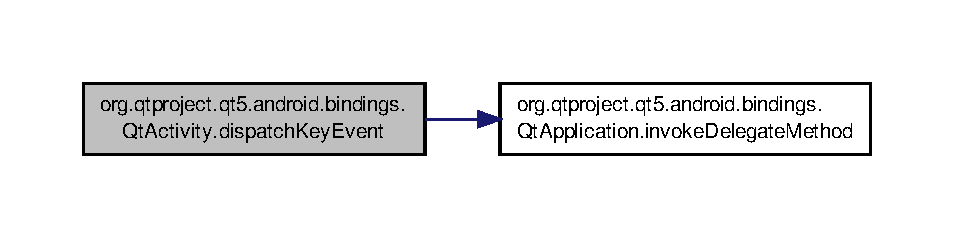
\includegraphics[width=350pt]{classorg_1_1qtproject_1_1qt5_1_1android_1_1bindings_1_1_qt_activity_a3419f10b60670ae0fd0a222fcd684273_cgraph}
\end{center}
\end{figure}


\hypertarget{classorg_1_1qtproject_1_1qt5_1_1android_1_1bindings_1_1_qt_activity_a7eacf9d228567bace814d7d90cc88dc1}{\index{org\-::qtproject\-::qt5\-::android\-::bindings\-::\-Qt\-Activity@{org\-::qtproject\-::qt5\-::android\-::bindings\-::\-Qt\-Activity}!dispatch\-Populate\-Accessibility\-Event@{dispatch\-Populate\-Accessibility\-Event}}
\index{dispatch\-Populate\-Accessibility\-Event@{dispatch\-Populate\-Accessibility\-Event}!org::qtproject::qt5::android::bindings::QtActivity@{org\-::qtproject\-::qt5\-::android\-::bindings\-::\-Qt\-Activity}}
\subsubsection[{dispatch\-Populate\-Accessibility\-Event}]{\setlength{\rightskip}{0pt plus 5cm}boolean org.\-qtproject.\-qt5.\-android.\-bindings.\-Qt\-Activity.\-dispatch\-Populate\-Accessibility\-Event (
\begin{DoxyParamCaption}
\item[{Accessibility\-Event}]{event}
\end{DoxyParamCaption}
)\hspace{0.3cm}{\ttfamily [inline]}}}\label{classorg_1_1qtproject_1_1qt5_1_1android_1_1bindings_1_1_qt_activity_a7eacf9d228567bace814d7d90cc88dc1}


Définition à la ligne 531 du fichier Qt\-Activity.\-java.



Voici le graphe d'appel pour cette fonction \-:\nopagebreak
\begin{figure}[H]
\begin{center}
\leavevmode
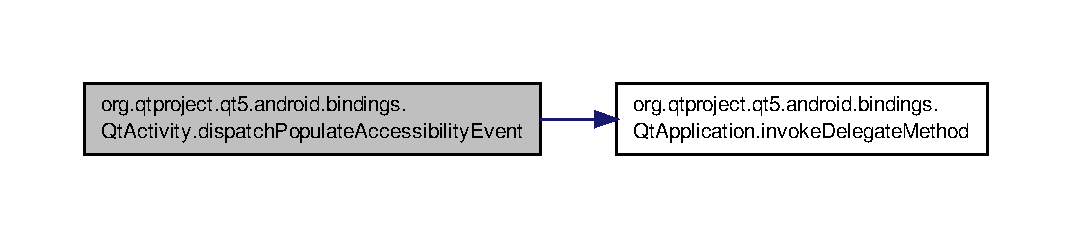
\includegraphics[width=350pt]{classorg_1_1qtproject_1_1qt5_1_1android_1_1bindings_1_1_qt_activity_a7eacf9d228567bace814d7d90cc88dc1_cgraph}
\end{center}
\end{figure}


\hypertarget{classorg_1_1qtproject_1_1qt5_1_1android_1_1bindings_1_1_qt_activity_a080d702cac33de4a97b4645567cf8c04}{\index{org\-::qtproject\-::qt5\-::android\-::bindings\-::\-Qt\-Activity@{org\-::qtproject\-::qt5\-::android\-::bindings\-::\-Qt\-Activity}!dispatch\-Touch\-Event@{dispatch\-Touch\-Event}}
\index{dispatch\-Touch\-Event@{dispatch\-Touch\-Event}!org::qtproject::qt5::android::bindings::QtActivity@{org\-::qtproject\-::qt5\-::android\-::bindings\-::\-Qt\-Activity}}
\subsubsection[{dispatch\-Touch\-Event}]{\setlength{\rightskip}{0pt plus 5cm}boolean org.\-qtproject.\-qt5.\-android.\-bindings.\-Qt\-Activity.\-dispatch\-Touch\-Event (
\begin{DoxyParamCaption}
\item[{Motion\-Event}]{ev}
\end{DoxyParamCaption}
)\hspace{0.3cm}{\ttfamily [inline]}}}\label{classorg_1_1qtproject_1_1qt5_1_1android_1_1bindings_1_1_qt_activity_a080d702cac33de4a97b4645567cf8c04}


Définition à la ligne 545 du fichier Qt\-Activity.\-java.



Voici le graphe d'appel pour cette fonction \-:\nopagebreak
\begin{figure}[H]
\begin{center}
\leavevmode
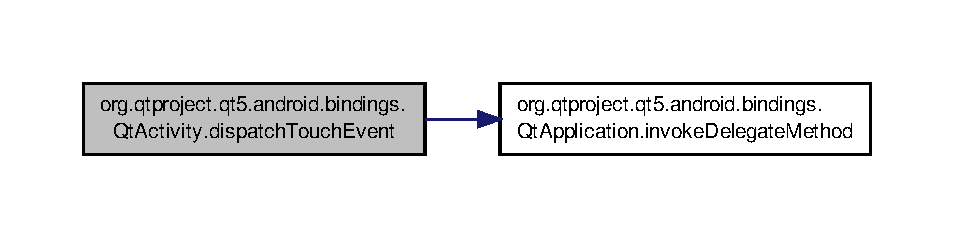
\includegraphics[width=350pt]{classorg_1_1qtproject_1_1qt5_1_1android_1_1bindings_1_1_qt_activity_a080d702cac33de4a97b4645567cf8c04_cgraph}
\end{center}
\end{figure}


\hypertarget{classorg_1_1qtproject_1_1qt5_1_1android_1_1bindings_1_1_qt_activity_ad305b6d78907e6fc4bc4fa9b77256a22}{\index{org\-::qtproject\-::qt5\-::android\-::bindings\-::\-Qt\-Activity@{org\-::qtproject\-::qt5\-::android\-::bindings\-::\-Qt\-Activity}!dispatch\-Trackball\-Event@{dispatch\-Trackball\-Event}}
\index{dispatch\-Trackball\-Event@{dispatch\-Trackball\-Event}!org::qtproject::qt5::android::bindings::QtActivity@{org\-::qtproject\-::qt5\-::android\-::bindings\-::\-Qt\-Activity}}
\subsubsection[{dispatch\-Trackball\-Event}]{\setlength{\rightskip}{0pt plus 5cm}boolean org.\-qtproject.\-qt5.\-android.\-bindings.\-Qt\-Activity.\-dispatch\-Trackball\-Event (
\begin{DoxyParamCaption}
\item[{Motion\-Event}]{ev}
\end{DoxyParamCaption}
)\hspace{0.3cm}{\ttfamily [inline]}}}\label{classorg_1_1qtproject_1_1qt5_1_1android_1_1bindings_1_1_qt_activity_ad305b6d78907e6fc4bc4fa9b77256a22}


Définition à la ligne 559 du fichier Qt\-Activity.\-java.



Voici le graphe d'appel pour cette fonction \-:\nopagebreak
\begin{figure}[H]
\begin{center}
\leavevmode
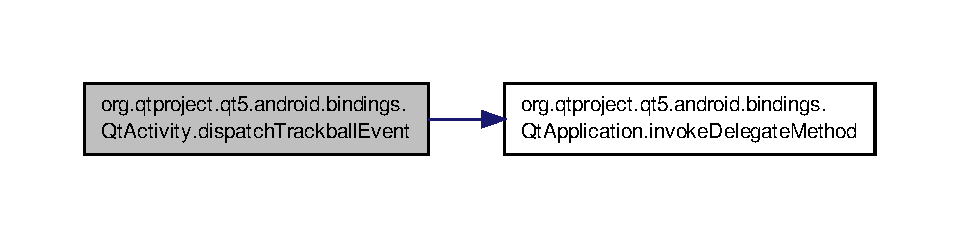
\includegraphics[width=350pt]{classorg_1_1qtproject_1_1qt5_1_1android_1_1bindings_1_1_qt_activity_ad305b6d78907e6fc4bc4fa9b77256a22_cgraph}
\end{center}
\end{figure}


\hypertarget{classorg_1_1qtproject_1_1qt5_1_1android_1_1bindings_1_1_qt_activity_abbade298e1a223acb5900e1ddd6ace74}{\index{org\-::qtproject\-::qt5\-::android\-::bindings\-::\-Qt\-Activity@{org\-::qtproject\-::qt5\-::android\-::bindings\-::\-Qt\-Activity}!download\-Upgrade\-Ministro@{download\-Upgrade\-Ministro}}
\index{download\-Upgrade\-Ministro@{download\-Upgrade\-Ministro}!org::qtproject::qt5::android::bindings::QtActivity@{org\-::qtproject\-::qt5\-::android\-::bindings\-::\-Qt\-Activity}}
\subsubsection[{download\-Upgrade\-Ministro}]{\setlength{\rightskip}{0pt plus 5cm}void org.\-qtproject.\-qt5.\-android.\-bindings.\-Qt\-Activity.\-download\-Upgrade\-Ministro (
\begin{DoxyParamCaption}
\item[{String}]{msg}
\end{DoxyParamCaption}
)\hspace{0.3cm}{\ttfamily [inline]}, {\ttfamily [private]}}}\label{classorg_1_1qtproject_1_1qt5_1_1android_1_1bindings_1_1_qt_activity_abbade298e1a223acb5900e1ddd6ace74}


Définition à la ligne 276 du fichier Qt\-Activity.\-java.



Voici le graphe d'appel pour cette fonction \-:\nopagebreak
\begin{figure}[H]
\begin{center}
\leavevmode
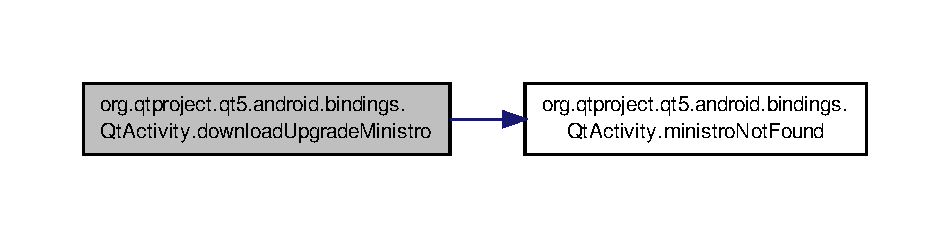
\includegraphics[width=350pt]{classorg_1_1qtproject_1_1qt5_1_1android_1_1bindings_1_1_qt_activity_abbade298e1a223acb5900e1ddd6ace74_cgraph}
\end{center}
\end{figure}




Voici le graphe des appelants de cette fonction \-:\nopagebreak
\begin{figure}[H]
\begin{center}
\leavevmode
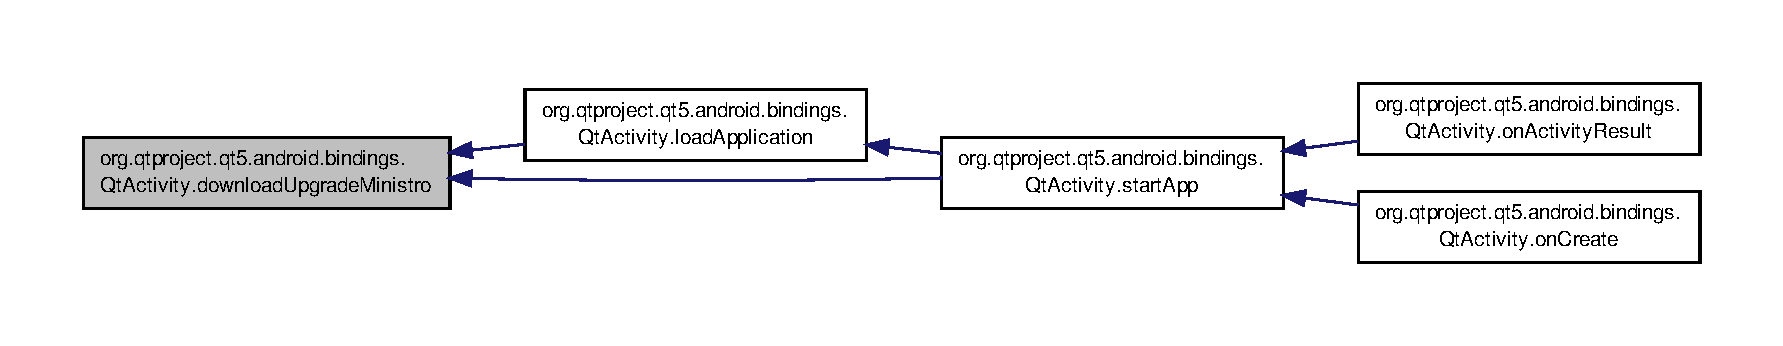
\includegraphics[width=350pt]{classorg_1_1qtproject_1_1qt5_1_1android_1_1bindings_1_1_qt_activity_abbade298e1a223acb5900e1ddd6ace74_icgraph}
\end{center}
\end{figure}


\hypertarget{classorg_1_1qtproject_1_1qt5_1_1android_1_1bindings_1_1_qt_activity_a38024ae043417efcc1b79aec389042b0}{\index{org\-::qtproject\-::qt5\-::android\-::bindings\-::\-Qt\-Activity@{org\-::qtproject\-::qt5\-::android\-::bindings\-::\-Qt\-Activity}!extract\-Bundled\-Plugins\-And\-Imports@{extract\-Bundled\-Plugins\-And\-Imports}}
\index{extract\-Bundled\-Plugins\-And\-Imports@{extract\-Bundled\-Plugins\-And\-Imports}!org::qtproject::qt5::android::bindings::QtActivity@{org\-::qtproject\-::qt5\-::android\-::bindings\-::\-Qt\-Activity}}
\subsubsection[{extract\-Bundled\-Plugins\-And\-Imports}]{\setlength{\rightskip}{0pt plus 5cm}void org.\-qtproject.\-qt5.\-android.\-bindings.\-Qt\-Activity.\-extract\-Bundled\-Plugins\-And\-Imports (
\begin{DoxyParamCaption}
\item[{String}]{local\-Prefix}
\end{DoxyParamCaption}
)  throws I\-O\-Exception     \hspace{0.3cm}{\ttfamily [inline]}, {\ttfamily [private]}}}\label{classorg_1_1qtproject_1_1qt5_1_1android_1_1bindings_1_1_qt_activity_a38024ae043417efcc1b79aec389042b0}


Définition à la ligne 371 du fichier Qt\-Activity.\-java.



Voici le graphe d'appel pour cette fonction \-:\nopagebreak
\begin{figure}[H]
\begin{center}
\leavevmode
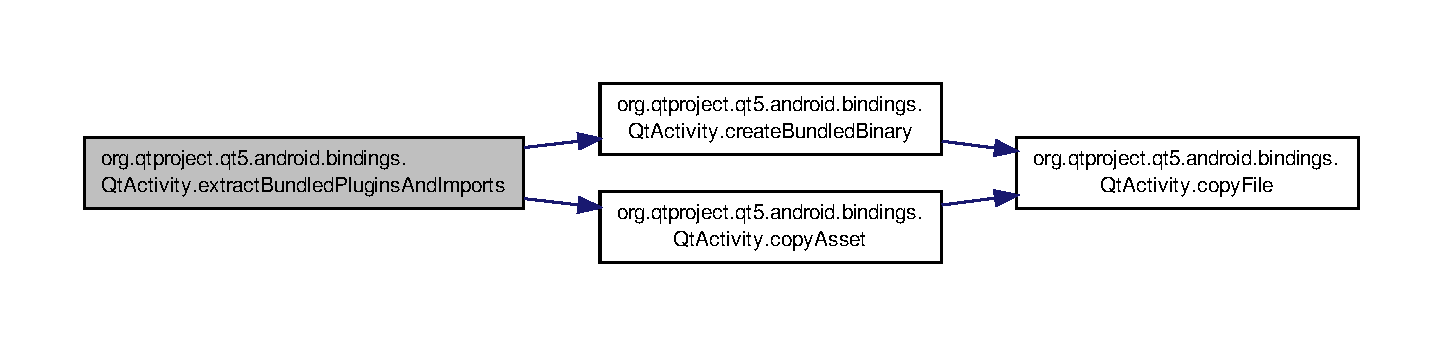
\includegraphics[width=350pt]{classorg_1_1qtproject_1_1qt5_1_1android_1_1bindings_1_1_qt_activity_a38024ae043417efcc1b79aec389042b0_cgraph}
\end{center}
\end{figure}




Voici le graphe des appelants de cette fonction \-:\nopagebreak
\begin{figure}[H]
\begin{center}
\leavevmode
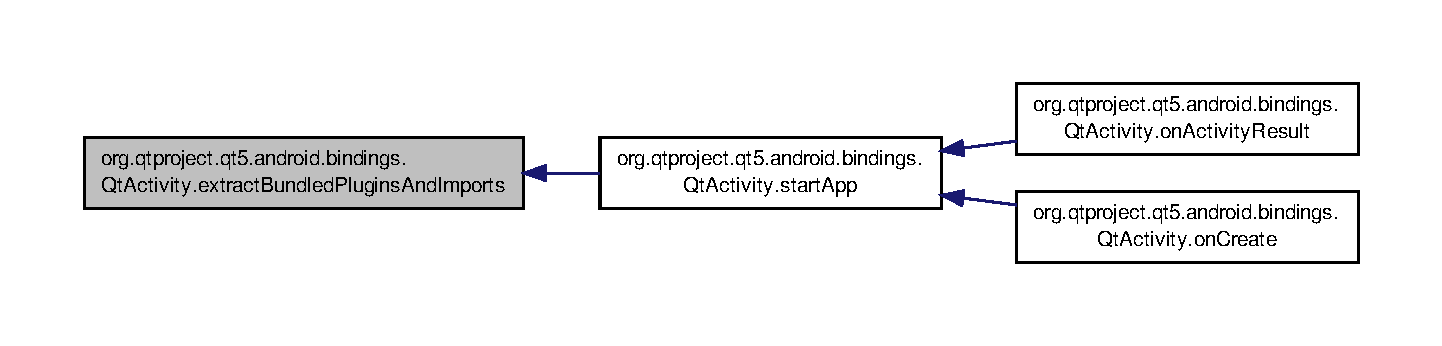
\includegraphics[width=350pt]{classorg_1_1qtproject_1_1qt5_1_1android_1_1bindings_1_1_qt_activity_a38024ae043417efcc1b79aec389042b0_icgraph}
\end{center}
\end{figure}


\hypertarget{classorg_1_1qtproject_1_1qt5_1_1android_1_1bindings_1_1_qt_activity_aa72e2a52d4667eac2de67b9148c5332b}{\index{org\-::qtproject\-::qt5\-::android\-::bindings\-::\-Qt\-Activity@{org\-::qtproject\-::qt5\-::android\-::bindings\-::\-Qt\-Activity}!load\-Application@{load\-Application}}
\index{load\-Application@{load\-Application}!org::qtproject::qt5::android::bindings::QtActivity@{org\-::qtproject\-::qt5\-::android\-::bindings\-::\-Qt\-Activity}}
\subsubsection[{load\-Application}]{\setlength{\rightskip}{0pt plus 5cm}void org.\-qtproject.\-qt5.\-android.\-bindings.\-Qt\-Activity.\-load\-Application (
\begin{DoxyParamCaption}
\item[{Bundle}]{loader\-Params}
\end{DoxyParamCaption}
)\hspace{0.3cm}{\ttfamily [inline]}, {\ttfamily [private]}}}\label{classorg_1_1qtproject_1_1qt5_1_1android_1_1bindings_1_1_qt_activity_aa72e2a52d4667eac2de67b9148c5332b}


Définition à la ligne 150 du fichier Qt\-Activity.\-java.



Voici le graphe d'appel pour cette fonction \-:\nopagebreak
\begin{figure}[H]
\begin{center}
\leavevmode
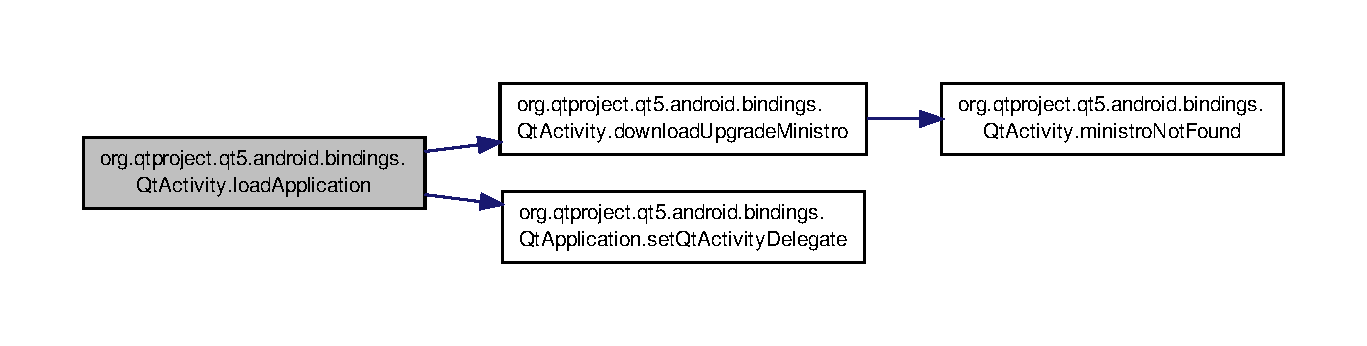
\includegraphics[width=350pt]{classorg_1_1qtproject_1_1qt5_1_1android_1_1bindings_1_1_qt_activity_aa72e2a52d4667eac2de67b9148c5332b_cgraph}
\end{center}
\end{figure}




Voici le graphe des appelants de cette fonction \-:\nopagebreak
\begin{figure}[H]
\begin{center}
\leavevmode
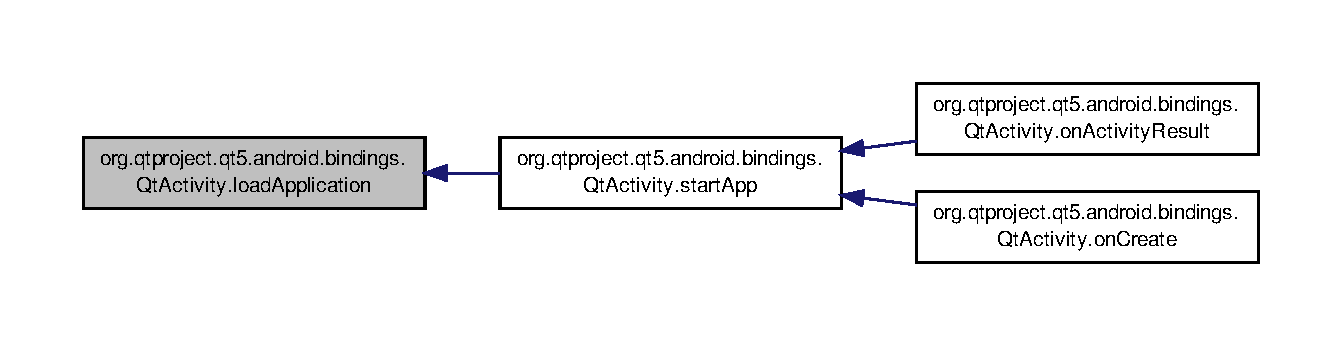
\includegraphics[width=350pt]{classorg_1_1qtproject_1_1qt5_1_1android_1_1bindings_1_1_qt_activity_aa72e2a52d4667eac2de67b9148c5332b_icgraph}
\end{center}
\end{figure}


\hypertarget{classorg_1_1qtproject_1_1qt5_1_1android_1_1bindings_1_1_qt_activity_a5e703f667905e2a0c11117197560d4e4}{\index{org\-::qtproject\-::qt5\-::android\-::bindings\-::\-Qt\-Activity@{org\-::qtproject\-::qt5\-::android\-::bindings\-::\-Qt\-Activity}!ministro\-Not\-Found@{ministro\-Not\-Found}}
\index{ministro\-Not\-Found@{ministro\-Not\-Found}!org::qtproject::qt5::android::bindings::QtActivity@{org\-::qtproject\-::qt5\-::android\-::bindings\-::\-Qt\-Activity}}
\subsubsection[{ministro\-Not\-Found}]{\setlength{\rightskip}{0pt plus 5cm}void org.\-qtproject.\-qt5.\-android.\-bindings.\-Qt\-Activity.\-ministro\-Not\-Found (
\begin{DoxyParamCaption}
{}
\end{DoxyParamCaption}
)\hspace{0.3cm}{\ttfamily [inline]}, {\ttfamily [private]}}}\label{classorg_1_1qtproject_1_1qt5_1_1android_1_1bindings_1_1_qt_activity_a5e703f667905e2a0c11117197560d4e4}


Définition à la ligne 303 du fichier Qt\-Activity.\-java.



Voici le graphe des appelants de cette fonction \-:\nopagebreak
\begin{figure}[H]
\begin{center}
\leavevmode
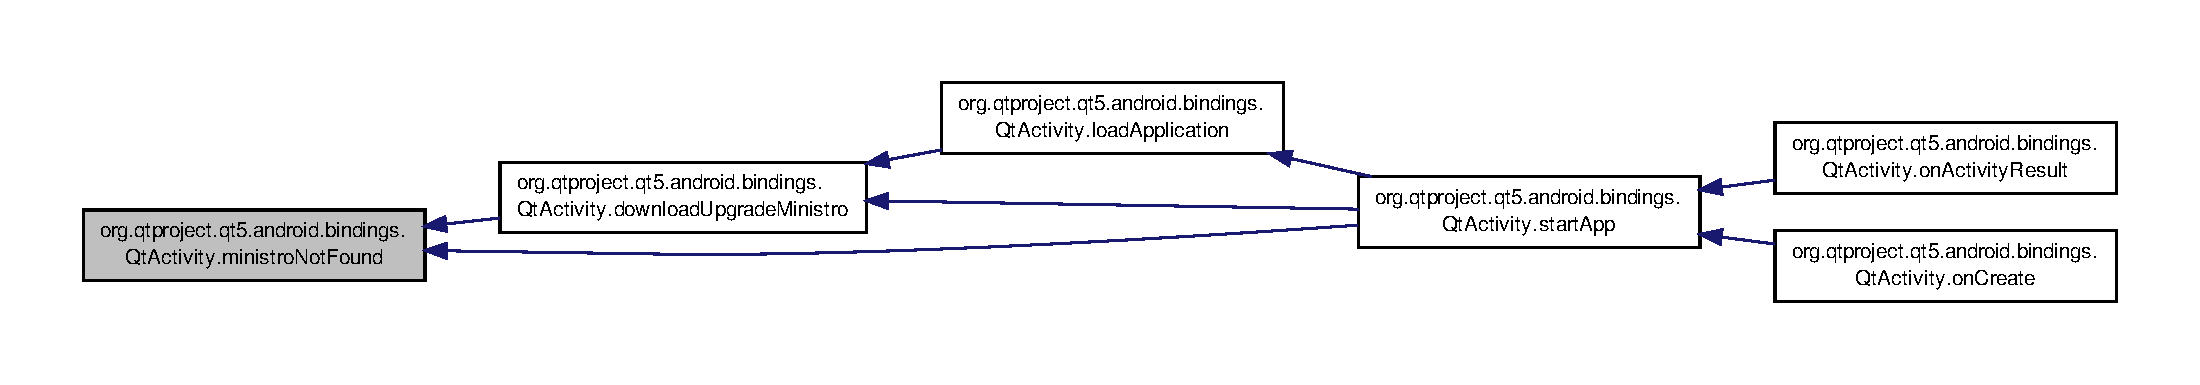
\includegraphics[width=350pt]{classorg_1_1qtproject_1_1qt5_1_1android_1_1bindings_1_1_qt_activity_a5e703f667905e2a0c11117197560d4e4_icgraph}
\end{center}
\end{figure}


\hypertarget{classorg_1_1qtproject_1_1qt5_1_1android_1_1bindings_1_1_qt_activity_a4e9a7c6b28384e4d5f713462207ffc41}{\index{org\-::qtproject\-::qt5\-::android\-::bindings\-::\-Qt\-Activity@{org\-::qtproject\-::qt5\-::android\-::bindings\-::\-Qt\-Activity}!on\-Activity\-Result@{on\-Activity\-Result}}
\index{on\-Activity\-Result@{on\-Activity\-Result}!org::qtproject::qt5::android::bindings::QtActivity@{org\-::qtproject\-::qt5\-::android\-::bindings\-::\-Qt\-Activity}}
\subsubsection[{on\-Activity\-Result}]{\setlength{\rightskip}{0pt plus 5cm}void org.\-qtproject.\-qt5.\-android.\-bindings.\-Qt\-Activity.\-on\-Activity\-Result (
\begin{DoxyParamCaption}
\item[{int}]{request\-Code, }
\item[{int}]{result\-Code, }
\item[{Intent}]{data}
\end{DoxyParamCaption}
)\hspace{0.3cm}{\ttfamily [inline]}, {\ttfamily [protected]}}}\label{classorg_1_1qtproject_1_1qt5_1_1android_1_1bindings_1_1_qt_activity_a4e9a7c6b28384e4d5f713462207ffc41}


Définition à la ligne 573 du fichier Qt\-Activity.\-java.



Voici le graphe d'appel pour cette fonction \-:\nopagebreak
\begin{figure}[H]
\begin{center}
\leavevmode
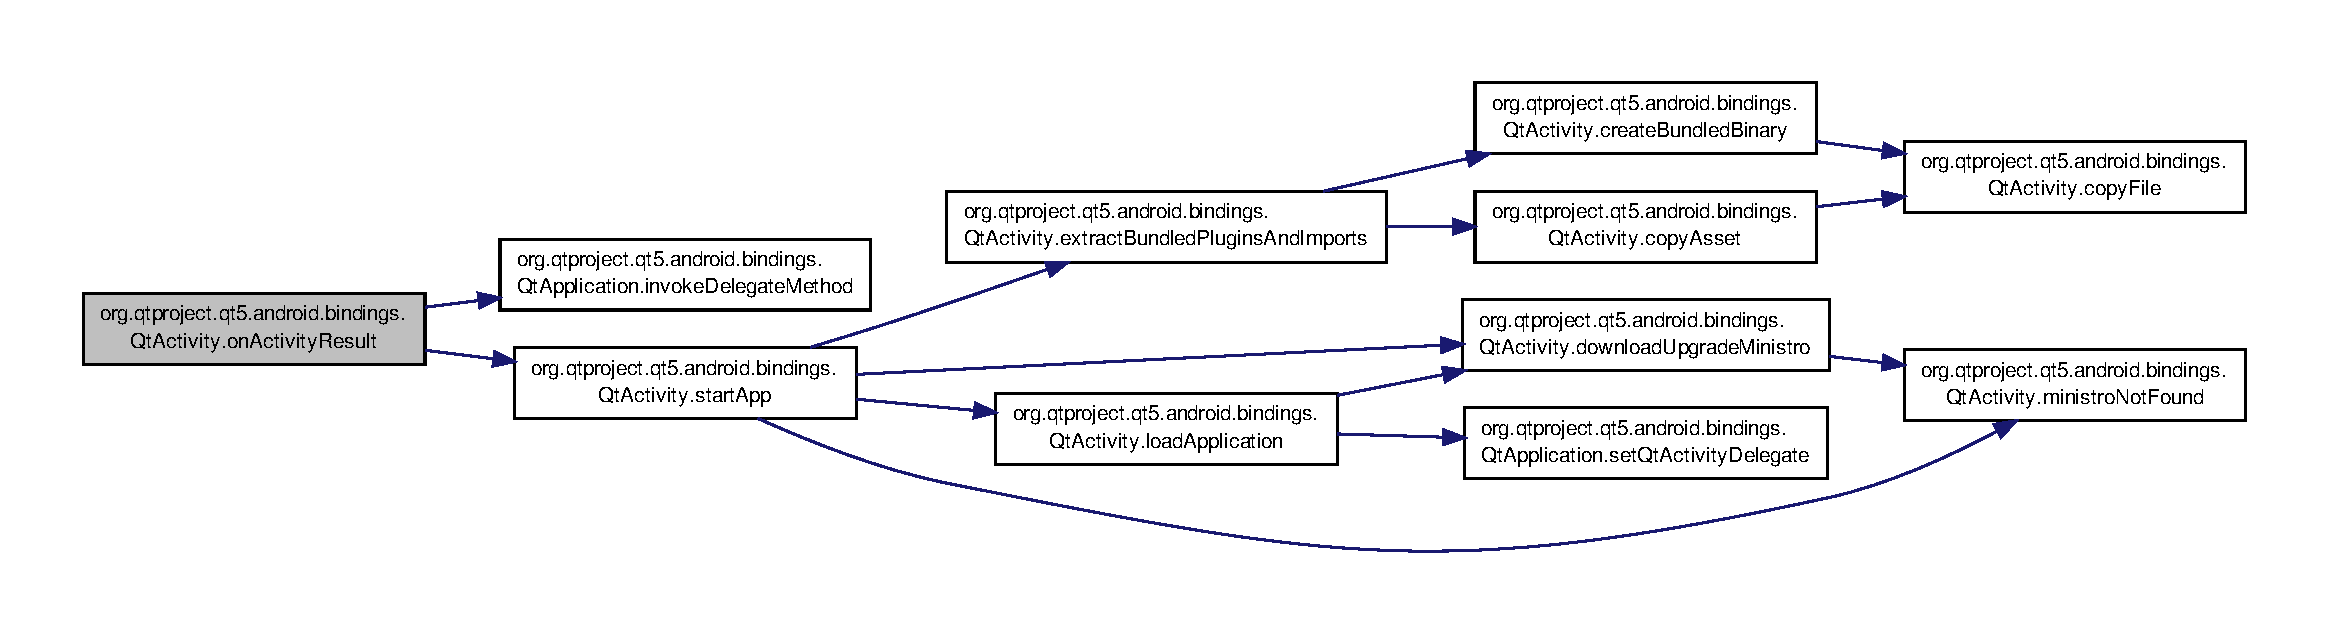
\includegraphics[width=350pt]{classorg_1_1qtproject_1_1qt5_1_1android_1_1bindings_1_1_qt_activity_a4e9a7c6b28384e4d5f713462207ffc41_cgraph}
\end{center}
\end{figure}


\hypertarget{classorg_1_1qtproject_1_1qt5_1_1android_1_1bindings_1_1_qt_activity_acd279279e5ad448d802fa31b64a30aef}{\index{org\-::qtproject\-::qt5\-::android\-::bindings\-::\-Qt\-Activity@{org\-::qtproject\-::qt5\-::android\-::bindings\-::\-Qt\-Activity}!on\-Apply\-Theme\-Resource@{on\-Apply\-Theme\-Resource}}
\index{on\-Apply\-Theme\-Resource@{on\-Apply\-Theme\-Resource}!org::qtproject::qt5::android::bindings::QtActivity@{org\-::qtproject\-::qt5\-::android\-::bindings\-::\-Qt\-Activity}}
\subsubsection[{on\-Apply\-Theme\-Resource}]{\setlength{\rightskip}{0pt plus 5cm}void org.\-qtproject.\-qt5.\-android.\-bindings.\-Qt\-Activity.\-on\-Apply\-Theme\-Resource (
\begin{DoxyParamCaption}
\item[{Theme}]{theme, }
\item[{int}]{resid, }
\item[{boolean}]{first}
\end{DoxyParamCaption}
)\hspace{0.3cm}{\ttfamily [inline]}, {\ttfamily [protected]}}}\label{classorg_1_1qtproject_1_1qt5_1_1android_1_1bindings_1_1_qt_activity_acd279279e5ad448d802fa31b64a30aef}


Définition à la ligne 591 du fichier Qt\-Activity.\-java.



Voici le graphe d'appel pour cette fonction \-:\nopagebreak
\begin{figure}[H]
\begin{center}
\leavevmode
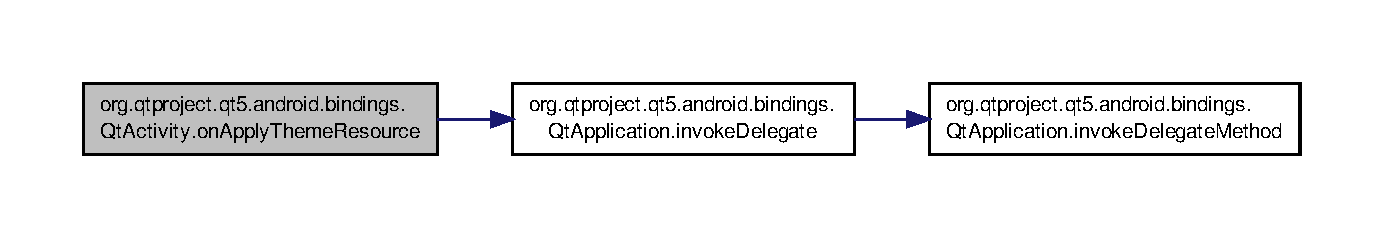
\includegraphics[width=350pt]{classorg_1_1qtproject_1_1qt5_1_1android_1_1bindings_1_1_qt_activity_acd279279e5ad448d802fa31b64a30aef_cgraph}
\end{center}
\end{figure}


\hypertarget{classorg_1_1qtproject_1_1qt5_1_1android_1_1bindings_1_1_qt_activity_a052fd4aee0de52bcf2d8a10c5671d586}{\index{org\-::qtproject\-::qt5\-::android\-::bindings\-::\-Qt\-Activity@{org\-::qtproject\-::qt5\-::android\-::bindings\-::\-Qt\-Activity}!on\-Attached\-To\-Window@{on\-Attached\-To\-Window}}
\index{on\-Attached\-To\-Window@{on\-Attached\-To\-Window}!org::qtproject::qt5::android::bindings::QtActivity@{org\-::qtproject\-::qt5\-::android\-::bindings\-::\-Qt\-Activity}}
\subsubsection[{on\-Attached\-To\-Window}]{\setlength{\rightskip}{0pt plus 5cm}void org.\-qtproject.\-qt5.\-android.\-bindings.\-Qt\-Activity.\-on\-Attached\-To\-Window (
\begin{DoxyParamCaption}
{}
\end{DoxyParamCaption}
)\hspace{0.3cm}{\ttfamily [inline]}}}\label{classorg_1_1qtproject_1_1qt5_1_1android_1_1bindings_1_1_qt_activity_a052fd4aee0de52bcf2d8a10c5671d586}


Définition à la ligne 1196 du fichier Qt\-Activity.\-java.



Voici le graphe d'appel pour cette fonction \-:\nopagebreak
\begin{figure}[H]
\begin{center}
\leavevmode
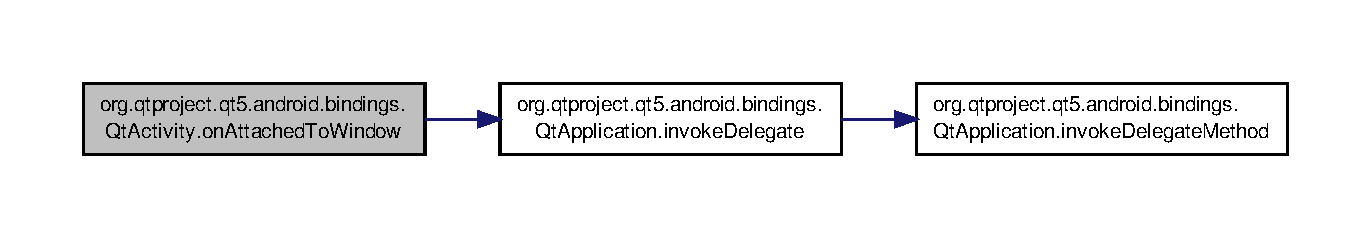
\includegraphics[width=350pt]{classorg_1_1qtproject_1_1qt5_1_1android_1_1bindings_1_1_qt_activity_a052fd4aee0de52bcf2d8a10c5671d586_cgraph}
\end{center}
\end{figure}


\hypertarget{classorg_1_1qtproject_1_1qt5_1_1android_1_1bindings_1_1_qt_activity_a593eeb49762865051c6348a6b98e7ff1}{\index{org\-::qtproject\-::qt5\-::android\-::bindings\-::\-Qt\-Activity@{org\-::qtproject\-::qt5\-::android\-::bindings\-::\-Qt\-Activity}!on\-Back\-Pressed@{on\-Back\-Pressed}}
\index{on\-Back\-Pressed@{on\-Back\-Pressed}!org::qtproject::qt5::android::bindings::QtActivity@{org\-::qtproject\-::qt5\-::android\-::bindings\-::\-Qt\-Activity}}
\subsubsection[{on\-Back\-Pressed}]{\setlength{\rightskip}{0pt plus 5cm}void org.\-qtproject.\-qt5.\-android.\-bindings.\-Qt\-Activity.\-on\-Back\-Pressed (
\begin{DoxyParamCaption}
{}
\end{DoxyParamCaption}
)\hspace{0.3cm}{\ttfamily [inline]}}}\label{classorg_1_1qtproject_1_1qt5_1_1android_1_1bindings_1_1_qt_activity_a593eeb49762865051c6348a6b98e7ff1}


Définition à la ligne 1208 du fichier Qt\-Activity.\-java.



Voici le graphe d'appel pour cette fonction \-:\nopagebreak
\begin{figure}[H]
\begin{center}
\leavevmode
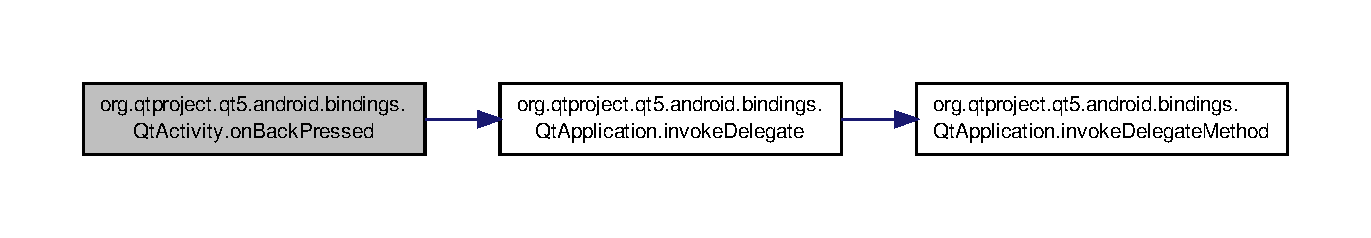
\includegraphics[width=350pt]{classorg_1_1qtproject_1_1qt5_1_1android_1_1bindings_1_1_qt_activity_a593eeb49762865051c6348a6b98e7ff1_cgraph}
\end{center}
\end{figure}


\hypertarget{classorg_1_1qtproject_1_1qt5_1_1android_1_1bindings_1_1_qt_activity_ac300f488c368a77573a3ecbf90f88b3c}{\index{org\-::qtproject\-::qt5\-::android\-::bindings\-::\-Qt\-Activity@{org\-::qtproject\-::qt5\-::android\-::bindings\-::\-Qt\-Activity}!on\-Child\-Title\-Changed@{on\-Child\-Title\-Changed}}
\index{on\-Child\-Title\-Changed@{on\-Child\-Title\-Changed}!org::qtproject::qt5::android::bindings::QtActivity@{org\-::qtproject\-::qt5\-::android\-::bindings\-::\-Qt\-Activity}}
\subsubsection[{on\-Child\-Title\-Changed}]{\setlength{\rightskip}{0pt plus 5cm}void org.\-qtproject.\-qt5.\-android.\-bindings.\-Qt\-Activity.\-on\-Child\-Title\-Changed (
\begin{DoxyParamCaption}
\item[{Activity}]{child\-Activity, }
\item[{Char\-Sequence}]{title}
\end{DoxyParamCaption}
)\hspace{0.3cm}{\ttfamily [inline]}, {\ttfamily [protected]}}}\label{classorg_1_1qtproject_1_1qt5_1_1android_1_1bindings_1_1_qt_activity_ac300f488c368a77573a3ecbf90f88b3c}


Définition à la ligne 604 du fichier Qt\-Activity.\-java.



Voici le graphe d'appel pour cette fonction \-:\nopagebreak
\begin{figure}[H]
\begin{center}
\leavevmode
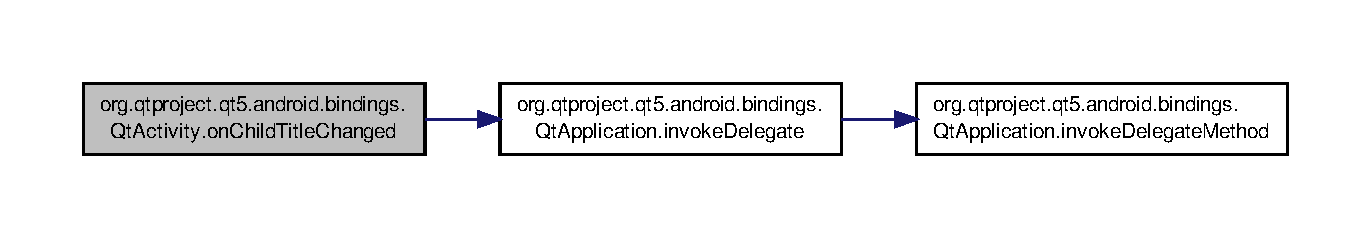
\includegraphics[width=350pt]{classorg_1_1qtproject_1_1qt5_1_1android_1_1bindings_1_1_qt_activity_ac300f488c368a77573a3ecbf90f88b3c_cgraph}
\end{center}
\end{figure}


\hypertarget{classorg_1_1qtproject_1_1qt5_1_1android_1_1bindings_1_1_qt_activity_a75ef70261caa7d4db3041147dc46c5d0}{\index{org\-::qtproject\-::qt5\-::android\-::bindings\-::\-Qt\-Activity@{org\-::qtproject\-::qt5\-::android\-::bindings\-::\-Qt\-Activity}!on\-Configuration\-Changed@{on\-Configuration\-Changed}}
\index{on\-Configuration\-Changed@{on\-Configuration\-Changed}!org::qtproject::qt5::android::bindings::QtActivity@{org\-::qtproject\-::qt5\-::android\-::bindings\-::\-Qt\-Activity}}
\subsubsection[{on\-Configuration\-Changed}]{\setlength{\rightskip}{0pt plus 5cm}void org.\-qtproject.\-qt5.\-android.\-bindings.\-Qt\-Activity.\-on\-Configuration\-Changed (
\begin{DoxyParamCaption}
\item[{Configuration}]{new\-Config}
\end{DoxyParamCaption}
)\hspace{0.3cm}{\ttfamily [inline]}}}\label{classorg_1_1qtproject_1_1qt5_1_1android_1_1bindings_1_1_qt_activity_a75ef70261caa7d4db3041147dc46c5d0}


Définition à la ligne 616 du fichier Qt\-Activity.\-java.



Voici le graphe d'appel pour cette fonction \-:\nopagebreak
\begin{figure}[H]
\begin{center}
\leavevmode
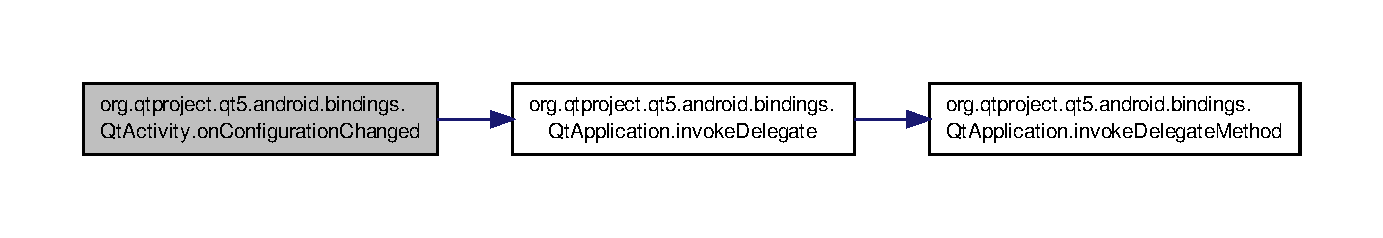
\includegraphics[width=350pt]{classorg_1_1qtproject_1_1qt5_1_1android_1_1bindings_1_1_qt_activity_a75ef70261caa7d4db3041147dc46c5d0_cgraph}
\end{center}
\end{figure}


\hypertarget{classorg_1_1qtproject_1_1qt5_1_1android_1_1bindings_1_1_qt_activity_a6310ffd404267a66b52dd4c3b357b560}{\index{org\-::qtproject\-::qt5\-::android\-::bindings\-::\-Qt\-Activity@{org\-::qtproject\-::qt5\-::android\-::bindings\-::\-Qt\-Activity}!on\-Content\-Changed@{on\-Content\-Changed}}
\index{on\-Content\-Changed@{on\-Content\-Changed}!org::qtproject::qt5::android::bindings::QtActivity@{org\-::qtproject\-::qt5\-::android\-::bindings\-::\-Qt\-Activity}}
\subsubsection[{on\-Content\-Changed}]{\setlength{\rightskip}{0pt plus 5cm}void org.\-qtproject.\-qt5.\-android.\-bindings.\-Qt\-Activity.\-on\-Content\-Changed (
\begin{DoxyParamCaption}
{}
\end{DoxyParamCaption}
)\hspace{0.3cm}{\ttfamily [inline]}}}\label{classorg_1_1qtproject_1_1qt5_1_1android_1_1bindings_1_1_qt_activity_a6310ffd404267a66b52dd4c3b357b560}


Définition à la ligne 628 du fichier Qt\-Activity.\-java.



Voici le graphe d'appel pour cette fonction \-:\nopagebreak
\begin{figure}[H]
\begin{center}
\leavevmode
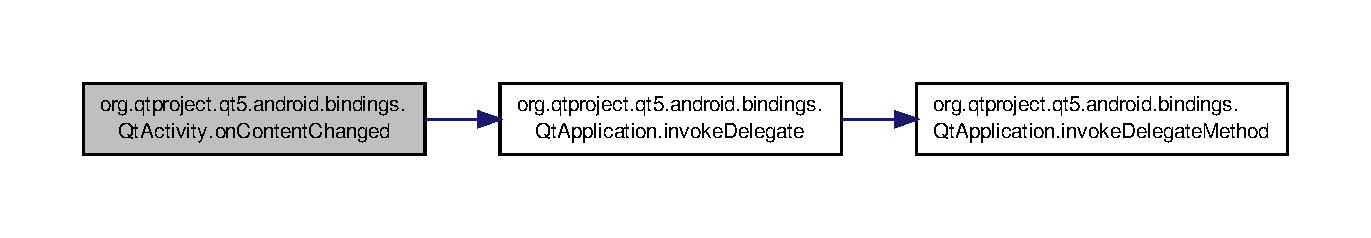
\includegraphics[width=350pt]{classorg_1_1qtproject_1_1qt5_1_1android_1_1bindings_1_1_qt_activity_a6310ffd404267a66b52dd4c3b357b560_cgraph}
\end{center}
\end{figure}


\hypertarget{classorg_1_1qtproject_1_1qt5_1_1android_1_1bindings_1_1_qt_activity_a67108692da62e48e5d02b22ed3d83769}{\index{org\-::qtproject\-::qt5\-::android\-::bindings\-::\-Qt\-Activity@{org\-::qtproject\-::qt5\-::android\-::bindings\-::\-Qt\-Activity}!on\-Context\-Item\-Selected@{on\-Context\-Item\-Selected}}
\index{on\-Context\-Item\-Selected@{on\-Context\-Item\-Selected}!org::qtproject::qt5::android::bindings::QtActivity@{org\-::qtproject\-::qt5\-::android\-::bindings\-::\-Qt\-Activity}}
\subsubsection[{on\-Context\-Item\-Selected}]{\setlength{\rightskip}{0pt plus 5cm}boolean org.\-qtproject.\-qt5.\-android.\-bindings.\-Qt\-Activity.\-on\-Context\-Item\-Selected (
\begin{DoxyParamCaption}
\item[{Menu\-Item}]{item}
\end{DoxyParamCaption}
)\hspace{0.3cm}{\ttfamily [inline]}}}\label{classorg_1_1qtproject_1_1qt5_1_1android_1_1bindings_1_1_qt_activity_a67108692da62e48e5d02b22ed3d83769}


Définition à la ligne 640 du fichier Qt\-Activity.\-java.



Voici le graphe d'appel pour cette fonction \-:\nopagebreak
\begin{figure}[H]
\begin{center}
\leavevmode
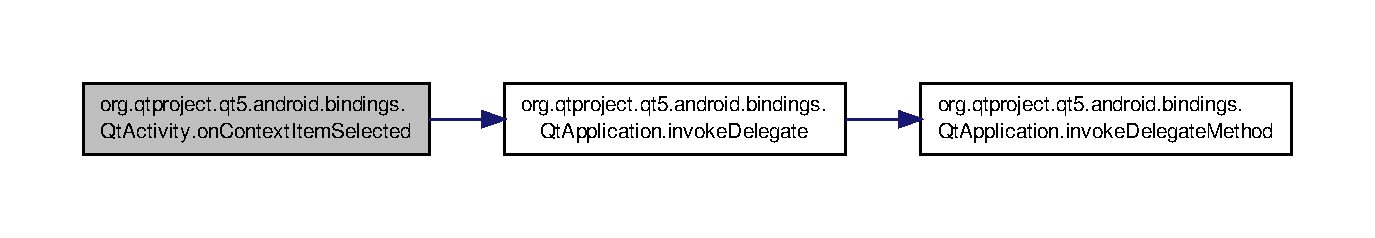
\includegraphics[width=350pt]{classorg_1_1qtproject_1_1qt5_1_1android_1_1bindings_1_1_qt_activity_a67108692da62e48e5d02b22ed3d83769_cgraph}
\end{center}
\end{figure}


\hypertarget{classorg_1_1qtproject_1_1qt5_1_1android_1_1bindings_1_1_qt_activity_a3e845800dc8fc21ff23589005d1a781c}{\index{org\-::qtproject\-::qt5\-::android\-::bindings\-::\-Qt\-Activity@{org\-::qtproject\-::qt5\-::android\-::bindings\-::\-Qt\-Activity}!on\-Context\-Menu\-Closed@{on\-Context\-Menu\-Closed}}
\index{on\-Context\-Menu\-Closed@{on\-Context\-Menu\-Closed}!org::qtproject::qt5::android::bindings::QtActivity@{org\-::qtproject\-::qt5\-::android\-::bindings\-::\-Qt\-Activity}}
\subsubsection[{on\-Context\-Menu\-Closed}]{\setlength{\rightskip}{0pt plus 5cm}void org.\-qtproject.\-qt5.\-android.\-bindings.\-Qt\-Activity.\-on\-Context\-Menu\-Closed (
\begin{DoxyParamCaption}
\item[{Menu}]{menu}
\end{DoxyParamCaption}
)\hspace{0.3cm}{\ttfamily [inline]}}}\label{classorg_1_1qtproject_1_1qt5_1_1android_1_1bindings_1_1_qt_activity_a3e845800dc8fc21ff23589005d1a781c}


Définition à la ligne 655 du fichier Qt\-Activity.\-java.



Voici le graphe d'appel pour cette fonction \-:\nopagebreak
\begin{figure}[H]
\begin{center}
\leavevmode
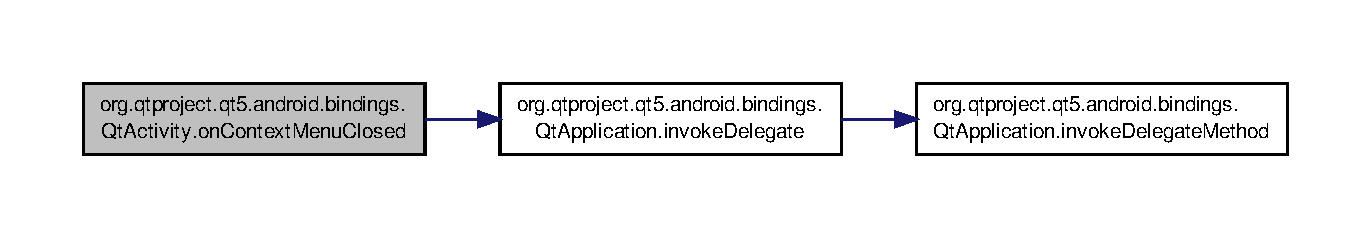
\includegraphics[width=350pt]{classorg_1_1qtproject_1_1qt5_1_1android_1_1bindings_1_1_qt_activity_a3e845800dc8fc21ff23589005d1a781c_cgraph}
\end{center}
\end{figure}


\hypertarget{classorg_1_1qtproject_1_1qt5_1_1android_1_1bindings_1_1_qt_activity_aa826639406d6f0697e0f1afcf69c748c}{\index{org\-::qtproject\-::qt5\-::android\-::bindings\-::\-Qt\-Activity@{org\-::qtproject\-::qt5\-::android\-::bindings\-::\-Qt\-Activity}!on\-Create@{on\-Create}}
\index{on\-Create@{on\-Create}!org::qtproject::qt5::android::bindings::QtActivity@{org\-::qtproject\-::qt5\-::android\-::bindings\-::\-Qt\-Activity}}
\subsubsection[{on\-Create}]{\setlength{\rightskip}{0pt plus 5cm}void org.\-qtproject.\-qt5.\-android.\-bindings.\-Qt\-Activity.\-on\-Create (
\begin{DoxyParamCaption}
\item[{Bundle}]{saved\-Instance\-State}
\end{DoxyParamCaption}
)\hspace{0.3cm}{\ttfamily [inline]}}}\label{classorg_1_1qtproject_1_1qt5_1_1android_1_1bindings_1_1_qt_activity_aa826639406d6f0697e0f1afcf69c748c}


Définition à la ligne 667 du fichier Qt\-Activity.\-java.



Voici le graphe d'appel pour cette fonction \-:\nopagebreak
\begin{figure}[H]
\begin{center}
\leavevmode
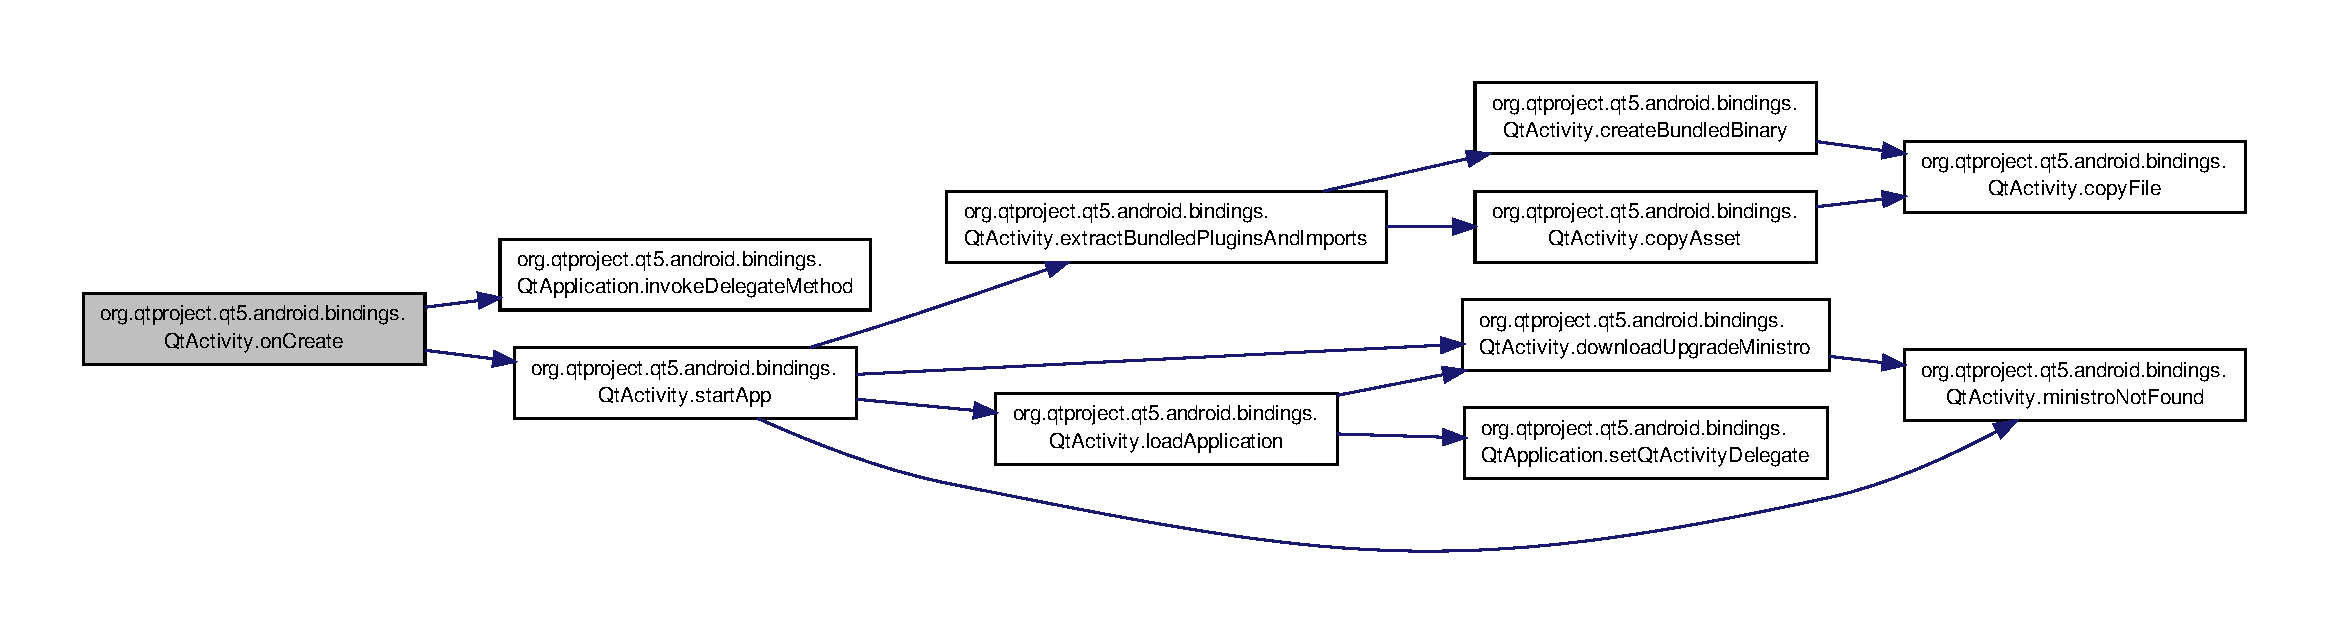
\includegraphics[width=350pt]{classorg_1_1qtproject_1_1qt5_1_1android_1_1bindings_1_1_qt_activity_aa826639406d6f0697e0f1afcf69c748c_cgraph}
\end{center}
\end{figure}


\hypertarget{classorg_1_1qtproject_1_1qt5_1_1android_1_1bindings_1_1_qt_activity_a924489f96650a755cf63980f3d388e8e}{\index{org\-::qtproject\-::qt5\-::android\-::bindings\-::\-Qt\-Activity@{org\-::qtproject\-::qt5\-::android\-::bindings\-::\-Qt\-Activity}!on\-Create\-Context\-Menu@{on\-Create\-Context\-Menu}}
\index{on\-Create\-Context\-Menu@{on\-Create\-Context\-Menu}!org::qtproject::qt5::android::bindings::QtActivity@{org\-::qtproject\-::qt5\-::android\-::bindings\-::\-Qt\-Activity}}
\subsubsection[{on\-Create\-Context\-Menu}]{\setlength{\rightskip}{0pt plus 5cm}void org.\-qtproject.\-qt5.\-android.\-bindings.\-Qt\-Activity.\-on\-Create\-Context\-Menu (
\begin{DoxyParamCaption}
\item[{Context\-Menu}]{menu, }
\item[{View}]{v, }
\item[{Context\-Menu\-Info}]{menu\-Info}
\end{DoxyParamCaption}
)\hspace{0.3cm}{\ttfamily [inline]}}}\label{classorg_1_1qtproject_1_1qt5_1_1android_1_1bindings_1_1_qt_activity_a924489f96650a755cf63980f3d388e8e}


Définition à la ligne 694 du fichier Qt\-Activity.\-java.



Voici le graphe d'appel pour cette fonction \-:\nopagebreak
\begin{figure}[H]
\begin{center}
\leavevmode
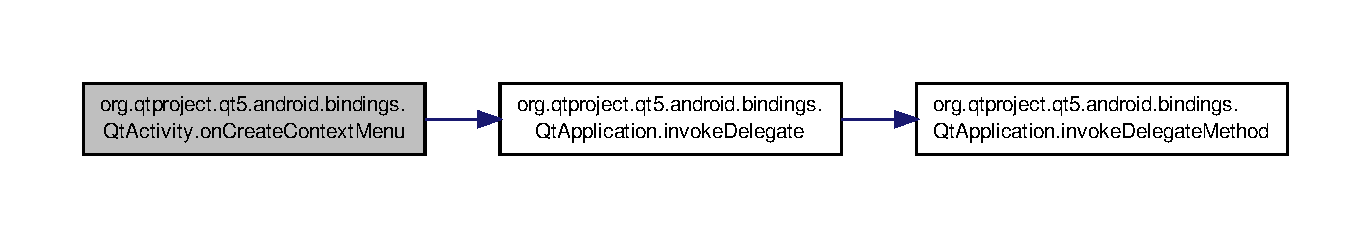
\includegraphics[width=350pt]{classorg_1_1qtproject_1_1qt5_1_1android_1_1bindings_1_1_qt_activity_a924489f96650a755cf63980f3d388e8e_cgraph}
\end{center}
\end{figure}


\hypertarget{classorg_1_1qtproject_1_1qt5_1_1android_1_1bindings_1_1_qt_activity_af86865337837c2c780913132b7118d69}{\index{org\-::qtproject\-::qt5\-::android\-::bindings\-::\-Qt\-Activity@{org\-::qtproject\-::qt5\-::android\-::bindings\-::\-Qt\-Activity}!on\-Create\-Description@{on\-Create\-Description}}
\index{on\-Create\-Description@{on\-Create\-Description}!org::qtproject::qt5::android::bindings::QtActivity@{org\-::qtproject\-::qt5\-::android\-::bindings\-::\-Qt\-Activity}}
\subsubsection[{on\-Create\-Description}]{\setlength{\rightskip}{0pt plus 5cm}Char\-Sequence org.\-qtproject.\-qt5.\-android.\-bindings.\-Qt\-Activity.\-on\-Create\-Description (
\begin{DoxyParamCaption}
{}
\end{DoxyParamCaption}
)\hspace{0.3cm}{\ttfamily [inline]}}}\label{classorg_1_1qtproject_1_1qt5_1_1android_1_1bindings_1_1_qt_activity_af86865337837c2c780913132b7118d69}


Définition à la ligne 706 du fichier Qt\-Activity.\-java.



Voici le graphe d'appel pour cette fonction \-:\nopagebreak
\begin{figure}[H]
\begin{center}
\leavevmode
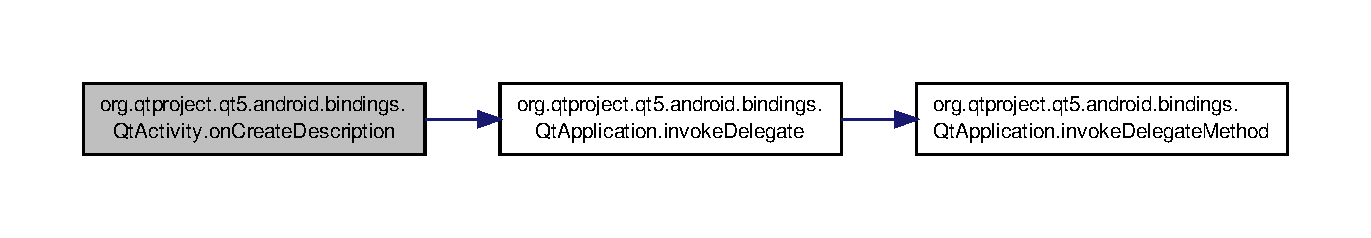
\includegraphics[width=350pt]{classorg_1_1qtproject_1_1qt5_1_1android_1_1bindings_1_1_qt_activity_af86865337837c2c780913132b7118d69_cgraph}
\end{center}
\end{figure}


\hypertarget{classorg_1_1qtproject_1_1qt5_1_1android_1_1bindings_1_1_qt_activity_a94b7cad79823109fd5ce75385766144b}{\index{org\-::qtproject\-::qt5\-::android\-::bindings\-::\-Qt\-Activity@{org\-::qtproject\-::qt5\-::android\-::bindings\-::\-Qt\-Activity}!on\-Create\-Dialog@{on\-Create\-Dialog}}
\index{on\-Create\-Dialog@{on\-Create\-Dialog}!org::qtproject::qt5::android::bindings::QtActivity@{org\-::qtproject\-::qt5\-::android\-::bindings\-::\-Qt\-Activity}}
\subsubsection[{on\-Create\-Dialog}]{\setlength{\rightskip}{0pt plus 5cm}Dialog org.\-qtproject.\-qt5.\-android.\-bindings.\-Qt\-Activity.\-on\-Create\-Dialog (
\begin{DoxyParamCaption}
\item[{int}]{id}
\end{DoxyParamCaption}
)\hspace{0.3cm}{\ttfamily [inline]}, {\ttfamily [protected]}}}\label{classorg_1_1qtproject_1_1qt5_1_1android_1_1bindings_1_1_qt_activity_a94b7cad79823109fd5ce75385766144b}


Définition à la ligne 721 du fichier Qt\-Activity.\-java.



Voici le graphe d'appel pour cette fonction \-:\nopagebreak
\begin{figure}[H]
\begin{center}
\leavevmode
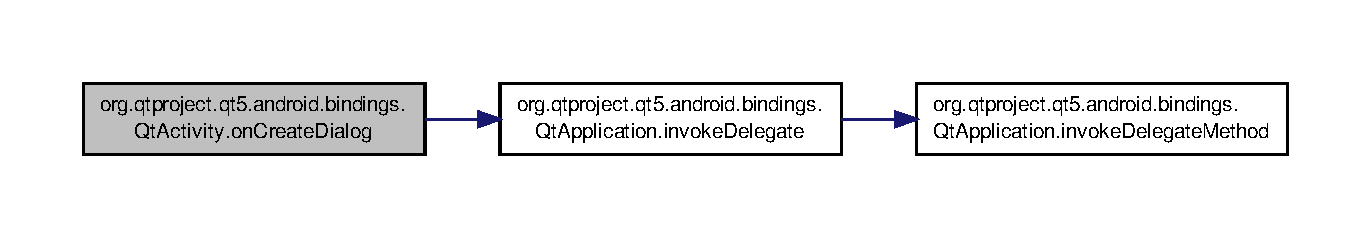
\includegraphics[width=350pt]{classorg_1_1qtproject_1_1qt5_1_1android_1_1bindings_1_1_qt_activity_a94b7cad79823109fd5ce75385766144b_cgraph}
\end{center}
\end{figure}


\hypertarget{classorg_1_1qtproject_1_1qt5_1_1android_1_1bindings_1_1_qt_activity_a68654d4382feda0419fd1a59792b3643}{\index{org\-::qtproject\-::qt5\-::android\-::bindings\-::\-Qt\-Activity@{org\-::qtproject\-::qt5\-::android\-::bindings\-::\-Qt\-Activity}!on\-Create\-Dialog@{on\-Create\-Dialog}}
\index{on\-Create\-Dialog@{on\-Create\-Dialog}!org::qtproject::qt5::android::bindings::QtActivity@{org\-::qtproject\-::qt5\-::android\-::bindings\-::\-Qt\-Activity}}
\subsubsection[{on\-Create\-Dialog}]{\setlength{\rightskip}{0pt plus 5cm}Dialog org.\-qtproject.\-qt5.\-android.\-bindings.\-Qt\-Activity.\-on\-Create\-Dialog (
\begin{DoxyParamCaption}
\item[{int}]{id, }
\item[{Bundle}]{args}
\end{DoxyParamCaption}
)\hspace{0.3cm}{\ttfamily [inline]}, {\ttfamily [protected]}}}\label{classorg_1_1qtproject_1_1qt5_1_1android_1_1bindings_1_1_qt_activity_a68654d4382feda0419fd1a59792b3643}


Définition à la ligne 1249 du fichier Qt\-Activity.\-java.



Voici le graphe d'appel pour cette fonction \-:\nopagebreak
\begin{figure}[H]
\begin{center}
\leavevmode
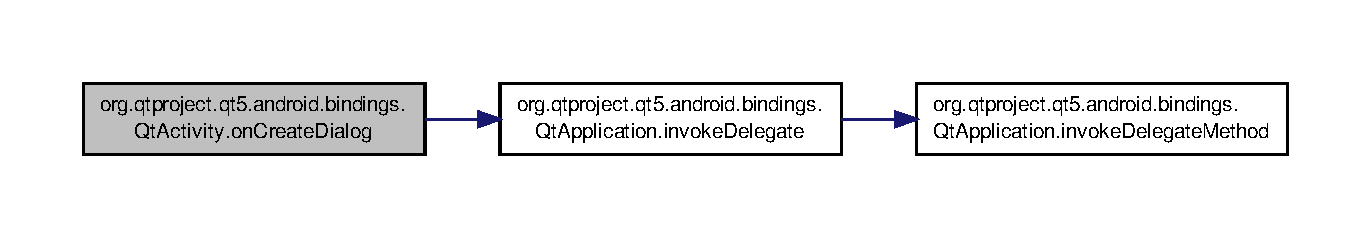
\includegraphics[width=350pt]{classorg_1_1qtproject_1_1qt5_1_1android_1_1bindings_1_1_qt_activity_a68654d4382feda0419fd1a59792b3643_cgraph}
\end{center}
\end{figure}


\hypertarget{classorg_1_1qtproject_1_1qt5_1_1android_1_1bindings_1_1_qt_activity_a9303a2dd16e8deb7cdcf143ae6b480f4}{\index{org\-::qtproject\-::qt5\-::android\-::bindings\-::\-Qt\-Activity@{org\-::qtproject\-::qt5\-::android\-::bindings\-::\-Qt\-Activity}!on\-Create\-Options\-Menu@{on\-Create\-Options\-Menu}}
\index{on\-Create\-Options\-Menu@{on\-Create\-Options\-Menu}!org::qtproject::qt5::android::bindings::QtActivity@{org\-::qtproject\-::qt5\-::android\-::bindings\-::\-Qt\-Activity}}
\subsubsection[{on\-Create\-Options\-Menu}]{\setlength{\rightskip}{0pt plus 5cm}boolean org.\-qtproject.\-qt5.\-android.\-bindings.\-Qt\-Activity.\-on\-Create\-Options\-Menu (
\begin{DoxyParamCaption}
\item[{Menu}]{menu}
\end{DoxyParamCaption}
)\hspace{0.3cm}{\ttfamily [inline]}}}\label{classorg_1_1qtproject_1_1qt5_1_1android_1_1bindings_1_1_qt_activity_a9303a2dd16e8deb7cdcf143ae6b480f4}


Définition à la ligne 736 du fichier Qt\-Activity.\-java.



Voici le graphe d'appel pour cette fonction \-:\nopagebreak
\begin{figure}[H]
\begin{center}
\leavevmode
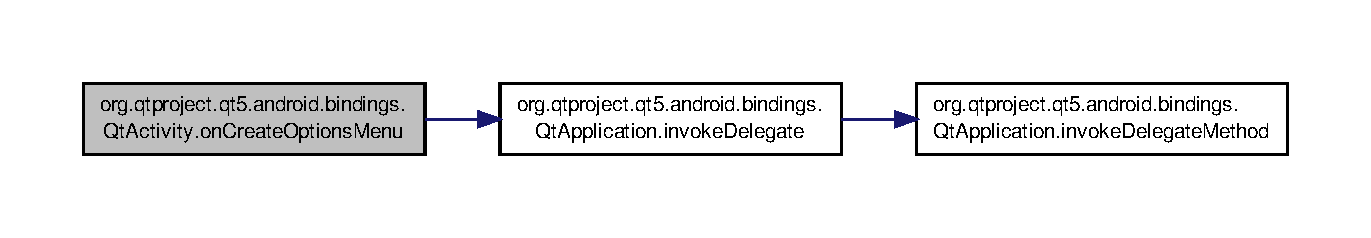
\includegraphics[width=350pt]{classorg_1_1qtproject_1_1qt5_1_1android_1_1bindings_1_1_qt_activity_a9303a2dd16e8deb7cdcf143ae6b480f4_cgraph}
\end{center}
\end{figure}


\hypertarget{classorg_1_1qtproject_1_1qt5_1_1android_1_1bindings_1_1_qt_activity_a617b7c2c432bc9894d3c0b2490d27b41}{\index{org\-::qtproject\-::qt5\-::android\-::bindings\-::\-Qt\-Activity@{org\-::qtproject\-::qt5\-::android\-::bindings\-::\-Qt\-Activity}!on\-Create\-Panel\-Menu@{on\-Create\-Panel\-Menu}}
\index{on\-Create\-Panel\-Menu@{on\-Create\-Panel\-Menu}!org::qtproject::qt5::android::bindings::QtActivity@{org\-::qtproject\-::qt5\-::android\-::bindings\-::\-Qt\-Activity}}
\subsubsection[{on\-Create\-Panel\-Menu}]{\setlength{\rightskip}{0pt plus 5cm}boolean org.\-qtproject.\-qt5.\-android.\-bindings.\-Qt\-Activity.\-on\-Create\-Panel\-Menu (
\begin{DoxyParamCaption}
\item[{int}]{feature\-Id, }
\item[{Menu}]{menu}
\end{DoxyParamCaption}
)\hspace{0.3cm}{\ttfamily [inline]}}}\label{classorg_1_1qtproject_1_1qt5_1_1android_1_1bindings_1_1_qt_activity_a617b7c2c432bc9894d3c0b2490d27b41}


Définition à la ligne 751 du fichier Qt\-Activity.\-java.



Voici le graphe d'appel pour cette fonction \-:\nopagebreak
\begin{figure}[H]
\begin{center}
\leavevmode
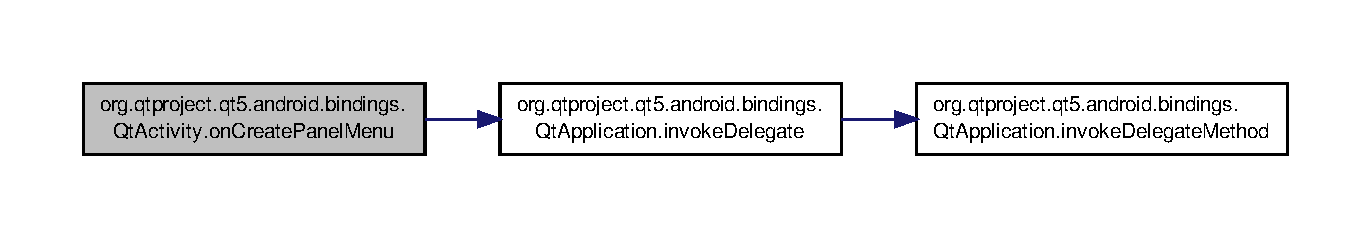
\includegraphics[width=350pt]{classorg_1_1qtproject_1_1qt5_1_1android_1_1bindings_1_1_qt_activity_a617b7c2c432bc9894d3c0b2490d27b41_cgraph}
\end{center}
\end{figure}


\hypertarget{classorg_1_1qtproject_1_1qt5_1_1android_1_1bindings_1_1_qt_activity_aefde1977c2ccae37e5f1a927f7e9e9ee}{\index{org\-::qtproject\-::qt5\-::android\-::bindings\-::\-Qt\-Activity@{org\-::qtproject\-::qt5\-::android\-::bindings\-::\-Qt\-Activity}!on\-Create\-Panel\-View@{on\-Create\-Panel\-View}}
\index{on\-Create\-Panel\-View@{on\-Create\-Panel\-View}!org::qtproject::qt5::android::bindings::QtActivity@{org\-::qtproject\-::qt5\-::android\-::bindings\-::\-Qt\-Activity}}
\subsubsection[{on\-Create\-Panel\-View}]{\setlength{\rightskip}{0pt plus 5cm}View org.\-qtproject.\-qt5.\-android.\-bindings.\-Qt\-Activity.\-on\-Create\-Panel\-View (
\begin{DoxyParamCaption}
\item[{int}]{feature\-Id}
\end{DoxyParamCaption}
)\hspace{0.3cm}{\ttfamily [inline]}}}\label{classorg_1_1qtproject_1_1qt5_1_1android_1_1bindings_1_1_qt_activity_aefde1977c2ccae37e5f1a927f7e9e9ee}


Définition à la ligne 767 du fichier Qt\-Activity.\-java.



Voici le graphe d'appel pour cette fonction \-:\nopagebreak
\begin{figure}[H]
\begin{center}
\leavevmode
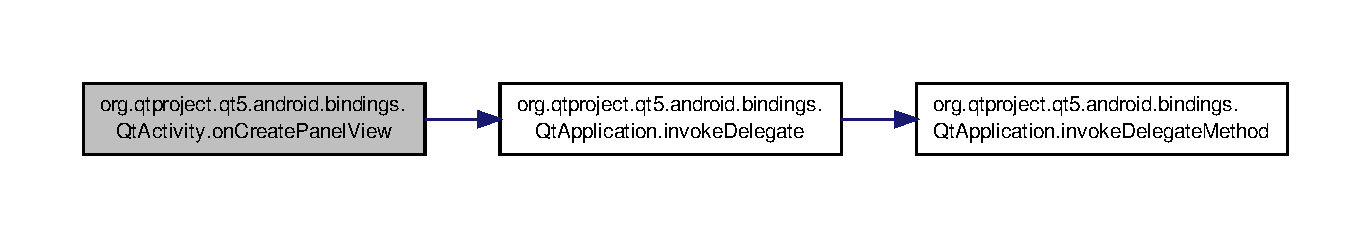
\includegraphics[width=350pt]{classorg_1_1qtproject_1_1qt5_1_1android_1_1bindings_1_1_qt_activity_aefde1977c2ccae37e5f1a927f7e9e9ee_cgraph}
\end{center}
\end{figure}


\hypertarget{classorg_1_1qtproject_1_1qt5_1_1android_1_1bindings_1_1_qt_activity_a961e15fb9b7bcdc7e4310e881656e1d7}{\index{org\-::qtproject\-::qt5\-::android\-::bindings\-::\-Qt\-Activity@{org\-::qtproject\-::qt5\-::android\-::bindings\-::\-Qt\-Activity}!on\-Create\-Thumbnail@{on\-Create\-Thumbnail}}
\index{on\-Create\-Thumbnail@{on\-Create\-Thumbnail}!org::qtproject::qt5::android::bindings::QtActivity@{org\-::qtproject\-::qt5\-::android\-::bindings\-::\-Qt\-Activity}}
\subsubsection[{on\-Create\-Thumbnail}]{\setlength{\rightskip}{0pt plus 5cm}boolean org.\-qtproject.\-qt5.\-android.\-bindings.\-Qt\-Activity.\-on\-Create\-Thumbnail (
\begin{DoxyParamCaption}
\item[{Bitmap}]{out\-Bitmap, }
\item[{Canvas}]{canvas}
\end{DoxyParamCaption}
)\hspace{0.3cm}{\ttfamily [inline]}}}\label{classorg_1_1qtproject_1_1qt5_1_1android_1_1bindings_1_1_qt_activity_a961e15fb9b7bcdc7e4310e881656e1d7}


Définition à la ligne 782 du fichier Qt\-Activity.\-java.



Voici le graphe d'appel pour cette fonction \-:\nopagebreak
\begin{figure}[H]
\begin{center}
\leavevmode
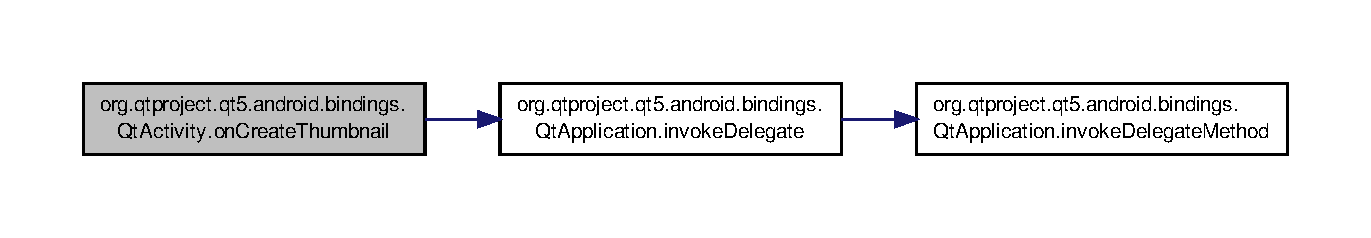
\includegraphics[width=350pt]{classorg_1_1qtproject_1_1qt5_1_1android_1_1bindings_1_1_qt_activity_a961e15fb9b7bcdc7e4310e881656e1d7_cgraph}
\end{center}
\end{figure}


\hypertarget{classorg_1_1qtproject_1_1qt5_1_1android_1_1bindings_1_1_qt_activity_a4f26e1f33245742068eb9b79689f69e5}{\index{org\-::qtproject\-::qt5\-::android\-::bindings\-::\-Qt\-Activity@{org\-::qtproject\-::qt5\-::android\-::bindings\-::\-Qt\-Activity}!on\-Create\-View@{on\-Create\-View}}
\index{on\-Create\-View@{on\-Create\-View}!org::qtproject::qt5::android::bindings::QtActivity@{org\-::qtproject\-::qt5\-::android\-::bindings\-::\-Qt\-Activity}}
\subsubsection[{on\-Create\-View}]{\setlength{\rightskip}{0pt plus 5cm}View org.\-qtproject.\-qt5.\-android.\-bindings.\-Qt\-Activity.\-on\-Create\-View (
\begin{DoxyParamCaption}
\item[{String}]{name, }
\item[{Context}]{context, }
\item[{Attribute\-Set}]{attrs}
\end{DoxyParamCaption}
)\hspace{0.3cm}{\ttfamily [inline]}}}\label{classorg_1_1qtproject_1_1qt5_1_1android_1_1bindings_1_1_qt_activity_a4f26e1f33245742068eb9b79689f69e5}


Définition à la ligne 797 du fichier Qt\-Activity.\-java.



Voici le graphe d'appel pour cette fonction \-:\nopagebreak
\begin{figure}[H]
\begin{center}
\leavevmode
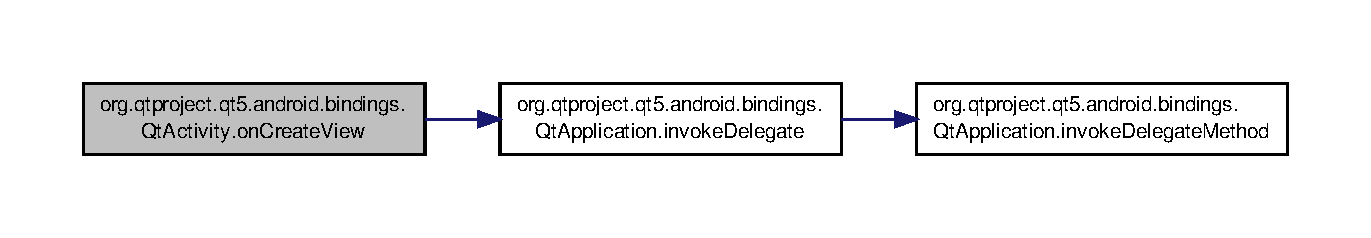
\includegraphics[width=350pt]{classorg_1_1qtproject_1_1qt5_1_1android_1_1bindings_1_1_qt_activity_a4f26e1f33245742068eb9b79689f69e5_cgraph}
\end{center}
\end{figure}


\hypertarget{classorg_1_1qtproject_1_1qt5_1_1android_1_1bindings_1_1_qt_activity_a30832553da49ca0dea222e062e21710c}{\index{org\-::qtproject\-::qt5\-::android\-::bindings\-::\-Qt\-Activity@{org\-::qtproject\-::qt5\-::android\-::bindings\-::\-Qt\-Activity}!on\-Destroy@{on\-Destroy}}
\index{on\-Destroy@{on\-Destroy}!org::qtproject::qt5::android::bindings::QtActivity@{org\-::qtproject\-::qt5\-::android\-::bindings\-::\-Qt\-Activity}}
\subsubsection[{on\-Destroy}]{\setlength{\rightskip}{0pt plus 5cm}void org.\-qtproject.\-qt5.\-android.\-bindings.\-Qt\-Activity.\-on\-Destroy (
\begin{DoxyParamCaption}
{}
\end{DoxyParamCaption}
)\hspace{0.3cm}{\ttfamily [inline]}, {\ttfamily [protected]}}}\label{classorg_1_1qtproject_1_1qt5_1_1android_1_1bindings_1_1_qt_activity_a30832553da49ca0dea222e062e21710c}


Définition à la ligne 812 du fichier Qt\-Activity.\-java.



Voici le graphe d'appel pour cette fonction \-:\nopagebreak
\begin{figure}[H]
\begin{center}
\leavevmode
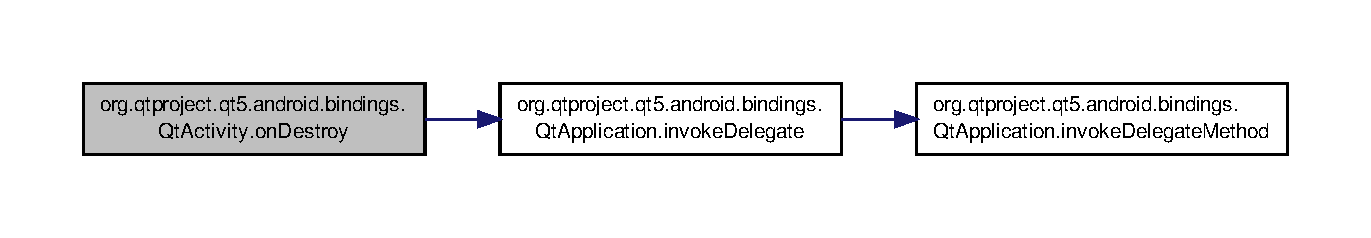
\includegraphics[width=350pt]{classorg_1_1qtproject_1_1qt5_1_1android_1_1bindings_1_1_qt_activity_a30832553da49ca0dea222e062e21710c_cgraph}
\end{center}
\end{figure}


\hypertarget{classorg_1_1qtproject_1_1qt5_1_1android_1_1bindings_1_1_qt_activity_aa7cad0cee8c325c1cbd7bb77a8a2c5ce}{\index{org\-::qtproject\-::qt5\-::android\-::bindings\-::\-Qt\-Activity@{org\-::qtproject\-::qt5\-::android\-::bindings\-::\-Qt\-Activity}!on\-Detached\-From\-Window@{on\-Detached\-From\-Window}}
\index{on\-Detached\-From\-Window@{on\-Detached\-From\-Window}!org::qtproject::qt5::android::bindings::QtActivity@{org\-::qtproject\-::qt5\-::android\-::bindings\-::\-Qt\-Activity}}
\subsubsection[{on\-Detached\-From\-Window}]{\setlength{\rightskip}{0pt plus 5cm}void org.\-qtproject.\-qt5.\-android.\-bindings.\-Qt\-Activity.\-on\-Detached\-From\-Window (
\begin{DoxyParamCaption}
{}
\end{DoxyParamCaption}
)\hspace{0.3cm}{\ttfamily [inline]}}}\label{classorg_1_1qtproject_1_1qt5_1_1android_1_1bindings_1_1_qt_activity_aa7cad0cee8c325c1cbd7bb77a8a2c5ce}


Définition à la ligne 1220 du fichier Qt\-Activity.\-java.



Voici le graphe d'appel pour cette fonction \-:\nopagebreak
\begin{figure}[H]
\begin{center}
\leavevmode
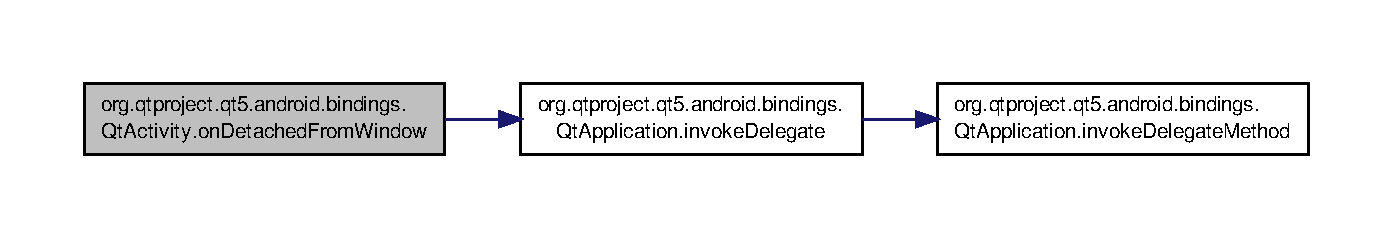
\includegraphics[width=350pt]{classorg_1_1qtproject_1_1qt5_1_1android_1_1bindings_1_1_qt_activity_aa7cad0cee8c325c1cbd7bb77a8a2c5ce_cgraph}
\end{center}
\end{figure}


\hypertarget{classorg_1_1qtproject_1_1qt5_1_1android_1_1bindings_1_1_qt_activity_ac1ee5a8d6b1ed5e7757139be8d7810be}{\index{org\-::qtproject\-::qt5\-::android\-::bindings\-::\-Qt\-Activity@{org\-::qtproject\-::qt5\-::android\-::bindings\-::\-Qt\-Activity}!on\-Key\-Down@{on\-Key\-Down}}
\index{on\-Key\-Down@{on\-Key\-Down}!org::qtproject::qt5::android::bindings::QtActivity@{org\-::qtproject\-::qt5\-::android\-::bindings\-::\-Qt\-Activity}}
\subsubsection[{on\-Key\-Down}]{\setlength{\rightskip}{0pt plus 5cm}boolean org.\-qtproject.\-qt5.\-android.\-bindings.\-Qt\-Activity.\-on\-Key\-Down (
\begin{DoxyParamCaption}
\item[{int}]{key\-Code, }
\item[{Key\-Event}]{event}
\end{DoxyParamCaption}
)\hspace{0.3cm}{\ttfamily [inline]}}}\label{classorg_1_1qtproject_1_1qt5_1_1android_1_1bindings_1_1_qt_activity_ac1ee5a8d6b1ed5e7757139be8d7810be}


Définition à la ligne 821 du fichier Qt\-Activity.\-java.



Voici le graphe d'appel pour cette fonction \-:\nopagebreak
\begin{figure}[H]
\begin{center}
\leavevmode
\includegraphics[width=350pt]{classorg_1_1qtproject_1_1qt5_1_1android_1_1bindings_1_1_qt_activity_ac1ee5a8d6b1ed5e7757139be8d7810be_cgraph}
\end{center}
\end{figure}


\hypertarget{classorg_1_1qtproject_1_1qt5_1_1android_1_1bindings_1_1_qt_activity_ad1c024d3096ee30566b083bf35b711f4}{\index{org\-::qtproject\-::qt5\-::android\-::bindings\-::\-Qt\-Activity@{org\-::qtproject\-::qt5\-::android\-::bindings\-::\-Qt\-Activity}!on\-Key\-Long\-Press@{on\-Key\-Long\-Press}}
\index{on\-Key\-Long\-Press@{on\-Key\-Long\-Press}!org::qtproject::qt5::android::bindings::QtActivity@{org\-::qtproject\-::qt5\-::android\-::bindings\-::\-Qt\-Activity}}
\subsubsection[{on\-Key\-Long\-Press}]{\setlength{\rightskip}{0pt plus 5cm}boolean org.\-qtproject.\-qt5.\-android.\-bindings.\-Qt\-Activity.\-on\-Key\-Long\-Press (
\begin{DoxyParamCaption}
\item[{int}]{key\-Code, }
\item[{Key\-Event}]{event}
\end{DoxyParamCaption}
)\hspace{0.3cm}{\ttfamily [inline]}}}\label{classorg_1_1qtproject_1_1qt5_1_1android_1_1bindings_1_1_qt_activity_ad1c024d3096ee30566b083bf35b711f4}


Définition à la ligne 1232 du fichier Qt\-Activity.\-java.



Voici le graphe d'appel pour cette fonction \-:\nopagebreak
\begin{figure}[H]
\begin{center}
\leavevmode
\includegraphics[width=350pt]{classorg_1_1qtproject_1_1qt5_1_1android_1_1bindings_1_1_qt_activity_ad1c024d3096ee30566b083bf35b711f4_cgraph}
\end{center}
\end{figure}


\hypertarget{classorg_1_1qtproject_1_1qt5_1_1android_1_1bindings_1_1_qt_activity_a9b41df58aada132667b9af5a8aa01aa7}{\index{org\-::qtproject\-::qt5\-::android\-::bindings\-::\-Qt\-Activity@{org\-::qtproject\-::qt5\-::android\-::bindings\-::\-Qt\-Activity}!on\-Key\-Multiple@{on\-Key\-Multiple}}
\index{on\-Key\-Multiple@{on\-Key\-Multiple}!org::qtproject::qt5::android::bindings::QtActivity@{org\-::qtproject\-::qt5\-::android\-::bindings\-::\-Qt\-Activity}}
\subsubsection[{on\-Key\-Multiple}]{\setlength{\rightskip}{0pt plus 5cm}boolean org.\-qtproject.\-qt5.\-android.\-bindings.\-Qt\-Activity.\-on\-Key\-Multiple (
\begin{DoxyParamCaption}
\item[{int}]{key\-Code, }
\item[{int}]{repeat\-Count, }
\item[{Key\-Event}]{event}
\end{DoxyParamCaption}
)\hspace{0.3cm}{\ttfamily [inline]}}}\label{classorg_1_1qtproject_1_1qt5_1_1android_1_1bindings_1_1_qt_activity_a9b41df58aada132667b9af5a8aa01aa7}


Définition à la ligne 836 du fichier Qt\-Activity.\-java.



Voici le graphe d'appel pour cette fonction \-:\nopagebreak
\begin{figure}[H]
\begin{center}
\leavevmode
\includegraphics[width=350pt]{classorg_1_1qtproject_1_1qt5_1_1android_1_1bindings_1_1_qt_activity_a9b41df58aada132667b9af5a8aa01aa7_cgraph}
\end{center}
\end{figure}


\hypertarget{classorg_1_1qtproject_1_1qt5_1_1android_1_1bindings_1_1_qt_activity_ac81bcf0a973ed2f8035bc3af8ee73f78}{\index{org\-::qtproject\-::qt5\-::android\-::bindings\-::\-Qt\-Activity@{org\-::qtproject\-::qt5\-::android\-::bindings\-::\-Qt\-Activity}!on\-Key\-Up@{on\-Key\-Up}}
\index{on\-Key\-Up@{on\-Key\-Up}!org::qtproject::qt5::android::bindings::QtActivity@{org\-::qtproject\-::qt5\-::android\-::bindings\-::\-Qt\-Activity}}
\subsubsection[{on\-Key\-Up}]{\setlength{\rightskip}{0pt plus 5cm}boolean org.\-qtproject.\-qt5.\-android.\-bindings.\-Qt\-Activity.\-on\-Key\-Up (
\begin{DoxyParamCaption}
\item[{int}]{key\-Code, }
\item[{Key\-Event}]{event}
\end{DoxyParamCaption}
)\hspace{0.3cm}{\ttfamily [inline]}}}\label{classorg_1_1qtproject_1_1qt5_1_1android_1_1bindings_1_1_qt_activity_ac81bcf0a973ed2f8035bc3af8ee73f78}


Définition à la ligne 850 du fichier Qt\-Activity.\-java.



Voici le graphe d'appel pour cette fonction \-:\nopagebreak
\begin{figure}[H]
\begin{center}
\leavevmode
\includegraphics[width=350pt]{classorg_1_1qtproject_1_1qt5_1_1android_1_1bindings_1_1_qt_activity_ac81bcf0a973ed2f8035bc3af8ee73f78_cgraph}
\end{center}
\end{figure}


\hypertarget{classorg_1_1qtproject_1_1qt5_1_1android_1_1bindings_1_1_qt_activity_a60dde1c5c76102c0514119fbc9515450}{\index{org\-::qtproject\-::qt5\-::android\-::bindings\-::\-Qt\-Activity@{org\-::qtproject\-::qt5\-::android\-::bindings\-::\-Qt\-Activity}!on\-Low\-Memory@{on\-Low\-Memory}}
\index{on\-Low\-Memory@{on\-Low\-Memory}!org::qtproject::qt5::android::bindings::QtActivity@{org\-::qtproject\-::qt5\-::android\-::bindings\-::\-Qt\-Activity}}
\subsubsection[{on\-Low\-Memory}]{\setlength{\rightskip}{0pt plus 5cm}void org.\-qtproject.\-qt5.\-android.\-bindings.\-Qt\-Activity.\-on\-Low\-Memory (
\begin{DoxyParamCaption}
{}
\end{DoxyParamCaption}
)\hspace{0.3cm}{\ttfamily [inline]}}}\label{classorg_1_1qtproject_1_1qt5_1_1android_1_1bindings_1_1_qt_activity_a60dde1c5c76102c0514119fbc9515450}


Définition à la ligne 864 du fichier Qt\-Activity.\-java.



Voici le graphe d'appel pour cette fonction \-:\nopagebreak
\begin{figure}[H]
\begin{center}
\leavevmode
\includegraphics[width=350pt]{classorg_1_1qtproject_1_1qt5_1_1android_1_1bindings_1_1_qt_activity_a60dde1c5c76102c0514119fbc9515450_cgraph}
\end{center}
\end{figure}


\hypertarget{classorg_1_1qtproject_1_1qt5_1_1android_1_1bindings_1_1_qt_activity_a15f3f492aba46975a36f1ebdfbe5ba45}{\index{org\-::qtproject\-::qt5\-::android\-::bindings\-::\-Qt\-Activity@{org\-::qtproject\-::qt5\-::android\-::bindings\-::\-Qt\-Activity}!on\-Menu\-Item\-Selected@{on\-Menu\-Item\-Selected}}
\index{on\-Menu\-Item\-Selected@{on\-Menu\-Item\-Selected}!org::qtproject::qt5::android::bindings::QtActivity@{org\-::qtproject\-::qt5\-::android\-::bindings\-::\-Qt\-Activity}}
\subsubsection[{on\-Menu\-Item\-Selected}]{\setlength{\rightskip}{0pt plus 5cm}boolean org.\-qtproject.\-qt5.\-android.\-bindings.\-Qt\-Activity.\-on\-Menu\-Item\-Selected (
\begin{DoxyParamCaption}
\item[{int}]{feature\-Id, }
\item[{Menu\-Item}]{item}
\end{DoxyParamCaption}
)\hspace{0.3cm}{\ttfamily [inline]}}}\label{classorg_1_1qtproject_1_1qt5_1_1android_1_1bindings_1_1_qt_activity_a15f3f492aba46975a36f1ebdfbe5ba45}


Définition à la ligne 872 du fichier Qt\-Activity.\-java.



Voici le graphe d'appel pour cette fonction \-:\nopagebreak
\begin{figure}[H]
\begin{center}
\leavevmode
\includegraphics[width=350pt]{classorg_1_1qtproject_1_1qt5_1_1android_1_1bindings_1_1_qt_activity_a15f3f492aba46975a36f1ebdfbe5ba45_cgraph}
\end{center}
\end{figure}


\hypertarget{classorg_1_1qtproject_1_1qt5_1_1android_1_1bindings_1_1_qt_activity_afa718d6a5777a519b1d513d7cbda938a}{\index{org\-::qtproject\-::qt5\-::android\-::bindings\-::\-Qt\-Activity@{org\-::qtproject\-::qt5\-::android\-::bindings\-::\-Qt\-Activity}!on\-Menu\-Opened@{on\-Menu\-Opened}}
\index{on\-Menu\-Opened@{on\-Menu\-Opened}!org::qtproject::qt5::android::bindings::QtActivity@{org\-::qtproject\-::qt5\-::android\-::bindings\-::\-Qt\-Activity}}
\subsubsection[{on\-Menu\-Opened}]{\setlength{\rightskip}{0pt plus 5cm}boolean org.\-qtproject.\-qt5.\-android.\-bindings.\-Qt\-Activity.\-on\-Menu\-Opened (
\begin{DoxyParamCaption}
\item[{int}]{feature\-Id, }
\item[{Menu}]{menu}
\end{DoxyParamCaption}
)\hspace{0.3cm}{\ttfamily [inline]}}}\label{classorg_1_1qtproject_1_1qt5_1_1android_1_1bindings_1_1_qt_activity_afa718d6a5777a519b1d513d7cbda938a}


Définition à la ligne 887 du fichier Qt\-Activity.\-java.



Voici le graphe d'appel pour cette fonction \-:\nopagebreak
\begin{figure}[H]
\begin{center}
\leavevmode
\includegraphics[width=350pt]{classorg_1_1qtproject_1_1qt5_1_1android_1_1bindings_1_1_qt_activity_afa718d6a5777a519b1d513d7cbda938a_cgraph}
\end{center}
\end{figure}


\hypertarget{classorg_1_1qtproject_1_1qt5_1_1android_1_1bindings_1_1_qt_activity_a995502b7cf803efcecc91d345b030404}{\index{org\-::qtproject\-::qt5\-::android\-::bindings\-::\-Qt\-Activity@{org\-::qtproject\-::qt5\-::android\-::bindings\-::\-Qt\-Activity}!on\-New\-Intent@{on\-New\-Intent}}
\index{on\-New\-Intent@{on\-New\-Intent}!org::qtproject::qt5::android::bindings::QtActivity@{org\-::qtproject\-::qt5\-::android\-::bindings\-::\-Qt\-Activity}}
\subsubsection[{on\-New\-Intent}]{\setlength{\rightskip}{0pt plus 5cm}void org.\-qtproject.\-qt5.\-android.\-bindings.\-Qt\-Activity.\-on\-New\-Intent (
\begin{DoxyParamCaption}
\item[{Intent}]{intent}
\end{DoxyParamCaption}
)\hspace{0.3cm}{\ttfamily [inline]}, {\ttfamily [protected]}}}\label{classorg_1_1qtproject_1_1qt5_1_1android_1_1bindings_1_1_qt_activity_a995502b7cf803efcecc91d345b030404}


Définition à la ligne 902 du fichier Qt\-Activity.\-java.



Voici le graphe d'appel pour cette fonction \-:\nopagebreak
\begin{figure}[H]
\begin{center}
\leavevmode
\includegraphics[width=350pt]{classorg_1_1qtproject_1_1qt5_1_1android_1_1bindings_1_1_qt_activity_a995502b7cf803efcecc91d345b030404_cgraph}
\end{center}
\end{figure}


\hypertarget{classorg_1_1qtproject_1_1qt5_1_1android_1_1bindings_1_1_qt_activity_a1062f0dfba41ba945835041b94bfe4fa}{\index{org\-::qtproject\-::qt5\-::android\-::bindings\-::\-Qt\-Activity@{org\-::qtproject\-::qt5\-::android\-::bindings\-::\-Qt\-Activity}!on\-Options\-Item\-Selected@{on\-Options\-Item\-Selected}}
\index{on\-Options\-Item\-Selected@{on\-Options\-Item\-Selected}!org::qtproject::qt5::android::bindings::QtActivity@{org\-::qtproject\-::qt5\-::android\-::bindings\-::\-Qt\-Activity}}
\subsubsection[{on\-Options\-Item\-Selected}]{\setlength{\rightskip}{0pt plus 5cm}boolean org.\-qtproject.\-qt5.\-android.\-bindings.\-Qt\-Activity.\-on\-Options\-Item\-Selected (
\begin{DoxyParamCaption}
\item[{Menu\-Item}]{item}
\end{DoxyParamCaption}
)\hspace{0.3cm}{\ttfamily [inline]}}}\label{classorg_1_1qtproject_1_1qt5_1_1android_1_1bindings_1_1_qt_activity_a1062f0dfba41ba945835041b94bfe4fa}


Définition à la ligne 914 du fichier Qt\-Activity.\-java.



Voici le graphe d'appel pour cette fonction \-:\nopagebreak
\begin{figure}[H]
\begin{center}
\leavevmode
\includegraphics[width=350pt]{classorg_1_1qtproject_1_1qt5_1_1android_1_1bindings_1_1_qt_activity_a1062f0dfba41ba945835041b94bfe4fa_cgraph}
\end{center}
\end{figure}


\hypertarget{classorg_1_1qtproject_1_1qt5_1_1android_1_1bindings_1_1_qt_activity_aad115f4cdaebb71916b85ac6309a83c4}{\index{org\-::qtproject\-::qt5\-::android\-::bindings\-::\-Qt\-Activity@{org\-::qtproject\-::qt5\-::android\-::bindings\-::\-Qt\-Activity}!on\-Options\-Menu\-Closed@{on\-Options\-Menu\-Closed}}
\index{on\-Options\-Menu\-Closed@{on\-Options\-Menu\-Closed}!org::qtproject::qt5::android::bindings::QtActivity@{org\-::qtproject\-::qt5\-::android\-::bindings\-::\-Qt\-Activity}}
\subsubsection[{on\-Options\-Menu\-Closed}]{\setlength{\rightskip}{0pt plus 5cm}void org.\-qtproject.\-qt5.\-android.\-bindings.\-Qt\-Activity.\-on\-Options\-Menu\-Closed (
\begin{DoxyParamCaption}
\item[{Menu}]{menu}
\end{DoxyParamCaption}
)\hspace{0.3cm}{\ttfamily [inline]}}}\label{classorg_1_1qtproject_1_1qt5_1_1android_1_1bindings_1_1_qt_activity_aad115f4cdaebb71916b85ac6309a83c4}


Définition à la ligne 929 du fichier Qt\-Activity.\-java.



Voici le graphe d'appel pour cette fonction \-:\nopagebreak
\begin{figure}[H]
\begin{center}
\leavevmode
\includegraphics[width=350pt]{classorg_1_1qtproject_1_1qt5_1_1android_1_1bindings_1_1_qt_activity_aad115f4cdaebb71916b85ac6309a83c4_cgraph}
\end{center}
\end{figure}


\hypertarget{classorg_1_1qtproject_1_1qt5_1_1android_1_1bindings_1_1_qt_activity_a2b39eac5b8b7003b20171ddce6b16e37}{\index{org\-::qtproject\-::qt5\-::android\-::bindings\-::\-Qt\-Activity@{org\-::qtproject\-::qt5\-::android\-::bindings\-::\-Qt\-Activity}!on\-Panel\-Closed@{on\-Panel\-Closed}}
\index{on\-Panel\-Closed@{on\-Panel\-Closed}!org::qtproject::qt5::android::bindings::QtActivity@{org\-::qtproject\-::qt5\-::android\-::bindings\-::\-Qt\-Activity}}
\subsubsection[{on\-Panel\-Closed}]{\setlength{\rightskip}{0pt plus 5cm}void org.\-qtproject.\-qt5.\-android.\-bindings.\-Qt\-Activity.\-on\-Panel\-Closed (
\begin{DoxyParamCaption}
\item[{int}]{feature\-Id, }
\item[{Menu}]{menu}
\end{DoxyParamCaption}
)\hspace{0.3cm}{\ttfamily [inline]}}}\label{classorg_1_1qtproject_1_1qt5_1_1android_1_1bindings_1_1_qt_activity_a2b39eac5b8b7003b20171ddce6b16e37}


Définition à la ligne 941 du fichier Qt\-Activity.\-java.



Voici le graphe d'appel pour cette fonction \-:\nopagebreak
\begin{figure}[H]
\begin{center}
\leavevmode
\includegraphics[width=350pt]{classorg_1_1qtproject_1_1qt5_1_1android_1_1bindings_1_1_qt_activity_a2b39eac5b8b7003b20171ddce6b16e37_cgraph}
\end{center}
\end{figure}


\hypertarget{classorg_1_1qtproject_1_1qt5_1_1android_1_1bindings_1_1_qt_activity_a54af4563a2a1f3ea73187c2e9b9b042c}{\index{org\-::qtproject\-::qt5\-::android\-::bindings\-::\-Qt\-Activity@{org\-::qtproject\-::qt5\-::android\-::bindings\-::\-Qt\-Activity}!on\-Pause@{on\-Pause}}
\index{on\-Pause@{on\-Pause}!org::qtproject::qt5::android::bindings::QtActivity@{org\-::qtproject\-::qt5\-::android\-::bindings\-::\-Qt\-Activity}}
\subsubsection[{on\-Pause}]{\setlength{\rightskip}{0pt plus 5cm}void org.\-qtproject.\-qt5.\-android.\-bindings.\-Qt\-Activity.\-on\-Pause (
\begin{DoxyParamCaption}
{}
\end{DoxyParamCaption}
)\hspace{0.3cm}{\ttfamily [inline]}, {\ttfamily [protected]}}}\label{classorg_1_1qtproject_1_1qt5_1_1android_1_1bindings_1_1_qt_activity_a54af4563a2a1f3ea73187c2e9b9b042c}


Définition à la ligne 953 du fichier Qt\-Activity.\-java.



Voici le graphe d'appel pour cette fonction \-:\nopagebreak
\begin{figure}[H]
\begin{center}
\leavevmode
\includegraphics[width=350pt]{classorg_1_1qtproject_1_1qt5_1_1android_1_1bindings_1_1_qt_activity_a54af4563a2a1f3ea73187c2e9b9b042c_cgraph}
\end{center}
\end{figure}


\hypertarget{classorg_1_1qtproject_1_1qt5_1_1android_1_1bindings_1_1_qt_activity_a1a206c815af224d5bf06e5c921f4fdd4}{\index{org\-::qtproject\-::qt5\-::android\-::bindings\-::\-Qt\-Activity@{org\-::qtproject\-::qt5\-::android\-::bindings\-::\-Qt\-Activity}!on\-Post\-Create@{on\-Post\-Create}}
\index{on\-Post\-Create@{on\-Post\-Create}!org::qtproject::qt5::android::bindings::QtActivity@{org\-::qtproject\-::qt5\-::android\-::bindings\-::\-Qt\-Activity}}
\subsubsection[{on\-Post\-Create}]{\setlength{\rightskip}{0pt plus 5cm}void org.\-qtproject.\-qt5.\-android.\-bindings.\-Qt\-Activity.\-on\-Post\-Create (
\begin{DoxyParamCaption}
\item[{Bundle}]{saved\-Instance\-State}
\end{DoxyParamCaption}
)\hspace{0.3cm}{\ttfamily [inline]}, {\ttfamily [protected]}}}\label{classorg_1_1qtproject_1_1qt5_1_1android_1_1bindings_1_1_qt_activity_a1a206c815af224d5bf06e5c921f4fdd4}


Définition à la ligne 961 du fichier Qt\-Activity.\-java.



Voici le graphe d'appel pour cette fonction \-:\nopagebreak
\begin{figure}[H]
\begin{center}
\leavevmode
\includegraphics[width=350pt]{classorg_1_1qtproject_1_1qt5_1_1android_1_1bindings_1_1_qt_activity_a1a206c815af224d5bf06e5c921f4fdd4_cgraph}
\end{center}
\end{figure}


\hypertarget{classorg_1_1qtproject_1_1qt5_1_1android_1_1bindings_1_1_qt_activity_af23189d66db86a4a4356af8481450fa1}{\index{org\-::qtproject\-::qt5\-::android\-::bindings\-::\-Qt\-Activity@{org\-::qtproject\-::qt5\-::android\-::bindings\-::\-Qt\-Activity}!on\-Post\-Resume@{on\-Post\-Resume}}
\index{on\-Post\-Resume@{on\-Post\-Resume}!org::qtproject::qt5::android::bindings::QtActivity@{org\-::qtproject\-::qt5\-::android\-::bindings\-::\-Qt\-Activity}}
\subsubsection[{on\-Post\-Resume}]{\setlength{\rightskip}{0pt plus 5cm}void org.\-qtproject.\-qt5.\-android.\-bindings.\-Qt\-Activity.\-on\-Post\-Resume (
\begin{DoxyParamCaption}
{}
\end{DoxyParamCaption}
)\hspace{0.3cm}{\ttfamily [inline]}, {\ttfamily [protected]}}}\label{classorg_1_1qtproject_1_1qt5_1_1android_1_1bindings_1_1_qt_activity_af23189d66db86a4a4356af8481450fa1}


Définition à la ligne 969 du fichier Qt\-Activity.\-java.



Voici le graphe d'appel pour cette fonction \-:\nopagebreak
\begin{figure}[H]
\begin{center}
\leavevmode
\includegraphics[width=350pt]{classorg_1_1qtproject_1_1qt5_1_1android_1_1bindings_1_1_qt_activity_af23189d66db86a4a4356af8481450fa1_cgraph}
\end{center}
\end{figure}


\hypertarget{classorg_1_1qtproject_1_1qt5_1_1android_1_1bindings_1_1_qt_activity_a7c23883f7117af2b20250150e032935d}{\index{org\-::qtproject\-::qt5\-::android\-::bindings\-::\-Qt\-Activity@{org\-::qtproject\-::qt5\-::android\-::bindings\-::\-Qt\-Activity}!on\-Prepare\-Dialog@{on\-Prepare\-Dialog}}
\index{on\-Prepare\-Dialog@{on\-Prepare\-Dialog}!org::qtproject::qt5::android::bindings::QtActivity@{org\-::qtproject\-::qt5\-::android\-::bindings\-::\-Qt\-Activity}}
\subsubsection[{on\-Prepare\-Dialog}]{\setlength{\rightskip}{0pt plus 5cm}void org.\-qtproject.\-qt5.\-android.\-bindings.\-Qt\-Activity.\-on\-Prepare\-Dialog (
\begin{DoxyParamCaption}
\item[{int}]{id, }
\item[{Dialog}]{dialog}
\end{DoxyParamCaption}
)\hspace{0.3cm}{\ttfamily [inline]}, {\ttfamily [protected]}}}\label{classorg_1_1qtproject_1_1qt5_1_1android_1_1bindings_1_1_qt_activity_a7c23883f7117af2b20250150e032935d}


Définition à la ligne 977 du fichier Qt\-Activity.\-java.



Voici le graphe d'appel pour cette fonction \-:\nopagebreak
\begin{figure}[H]
\begin{center}
\leavevmode
\includegraphics[width=350pt]{classorg_1_1qtproject_1_1qt5_1_1android_1_1bindings_1_1_qt_activity_a7c23883f7117af2b20250150e032935d_cgraph}
\end{center}
\end{figure}


\hypertarget{classorg_1_1qtproject_1_1qt5_1_1android_1_1bindings_1_1_qt_activity_aa4466dc136a61b68aaf83cf3a5a9827d}{\index{org\-::qtproject\-::qt5\-::android\-::bindings\-::\-Qt\-Activity@{org\-::qtproject\-::qt5\-::android\-::bindings\-::\-Qt\-Activity}!on\-Prepare\-Dialog@{on\-Prepare\-Dialog}}
\index{on\-Prepare\-Dialog@{on\-Prepare\-Dialog}!org::qtproject::qt5::android::bindings::QtActivity@{org\-::qtproject\-::qt5\-::android\-::bindings\-::\-Qt\-Activity}}
\subsubsection[{on\-Prepare\-Dialog}]{\setlength{\rightskip}{0pt plus 5cm}void org.\-qtproject.\-qt5.\-android.\-bindings.\-Qt\-Activity.\-on\-Prepare\-Dialog (
\begin{DoxyParamCaption}
\item[{int}]{id, }
\item[{Dialog}]{dialog, }
\item[{Bundle}]{args}
\end{DoxyParamCaption}
)\hspace{0.3cm}{\ttfamily [inline]}, {\ttfamily [protected]}}}\label{classorg_1_1qtproject_1_1qt5_1_1android_1_1bindings_1_1_qt_activity_aa4466dc136a61b68aaf83cf3a5a9827d}


Définition à la ligne 1264 du fichier Qt\-Activity.\-java.



Voici le graphe d'appel pour cette fonction \-:\nopagebreak
\begin{figure}[H]
\begin{center}
\leavevmode
\includegraphics[width=350pt]{classorg_1_1qtproject_1_1qt5_1_1android_1_1bindings_1_1_qt_activity_aa4466dc136a61b68aaf83cf3a5a9827d_cgraph}
\end{center}
\end{figure}


\hypertarget{classorg_1_1qtproject_1_1qt5_1_1android_1_1bindings_1_1_qt_activity_a71a7e747de798c51b6a385b5e8a99c61}{\index{org\-::qtproject\-::qt5\-::android\-::bindings\-::\-Qt\-Activity@{org\-::qtproject\-::qt5\-::android\-::bindings\-::\-Qt\-Activity}!on\-Prepare\-Options\-Menu@{on\-Prepare\-Options\-Menu}}
\index{on\-Prepare\-Options\-Menu@{on\-Prepare\-Options\-Menu}!org::qtproject::qt5::android::bindings::QtActivity@{org\-::qtproject\-::qt5\-::android\-::bindings\-::\-Qt\-Activity}}
\subsubsection[{on\-Prepare\-Options\-Menu}]{\setlength{\rightskip}{0pt plus 5cm}boolean org.\-qtproject.\-qt5.\-android.\-bindings.\-Qt\-Activity.\-on\-Prepare\-Options\-Menu (
\begin{DoxyParamCaption}
\item[{Menu}]{menu}
\end{DoxyParamCaption}
)\hspace{0.3cm}{\ttfamily [inline]}}}\label{classorg_1_1qtproject_1_1qt5_1_1android_1_1bindings_1_1_qt_activity_a71a7e747de798c51b6a385b5e8a99c61}


Définition à la ligne 989 du fichier Qt\-Activity.\-java.



Voici le graphe d'appel pour cette fonction \-:\nopagebreak
\begin{figure}[H]
\begin{center}
\leavevmode
\includegraphics[width=350pt]{classorg_1_1qtproject_1_1qt5_1_1android_1_1bindings_1_1_qt_activity_a71a7e747de798c51b6a385b5e8a99c61_cgraph}
\end{center}
\end{figure}


\hypertarget{classorg_1_1qtproject_1_1qt5_1_1android_1_1bindings_1_1_qt_activity_a668c15554849a0bce9422eb709b5cacc}{\index{org\-::qtproject\-::qt5\-::android\-::bindings\-::\-Qt\-Activity@{org\-::qtproject\-::qt5\-::android\-::bindings\-::\-Qt\-Activity}!on\-Prepare\-Panel@{on\-Prepare\-Panel}}
\index{on\-Prepare\-Panel@{on\-Prepare\-Panel}!org::qtproject::qt5::android::bindings::QtActivity@{org\-::qtproject\-::qt5\-::android\-::bindings\-::\-Qt\-Activity}}
\subsubsection[{on\-Prepare\-Panel}]{\setlength{\rightskip}{0pt plus 5cm}boolean org.\-qtproject.\-qt5.\-android.\-bindings.\-Qt\-Activity.\-on\-Prepare\-Panel (
\begin{DoxyParamCaption}
\item[{int}]{feature\-Id, }
\item[{View}]{view, }
\item[{Menu}]{menu}
\end{DoxyParamCaption}
)\hspace{0.3cm}{\ttfamily [inline]}}}\label{classorg_1_1qtproject_1_1qt5_1_1android_1_1bindings_1_1_qt_activity_a668c15554849a0bce9422eb709b5cacc}


Définition à la ligne 1004 du fichier Qt\-Activity.\-java.



Voici le graphe d'appel pour cette fonction \-:\nopagebreak
\begin{figure}[H]
\begin{center}
\leavevmode
\includegraphics[width=350pt]{classorg_1_1qtproject_1_1qt5_1_1android_1_1bindings_1_1_qt_activity_a668c15554849a0bce9422eb709b5cacc_cgraph}
\end{center}
\end{figure}


\hypertarget{classorg_1_1qtproject_1_1qt5_1_1android_1_1bindings_1_1_qt_activity_a05a1cabee75d99161959de7575052b73}{\index{org\-::qtproject\-::qt5\-::android\-::bindings\-::\-Qt\-Activity@{org\-::qtproject\-::qt5\-::android\-::bindings\-::\-Qt\-Activity}!on\-Restart@{on\-Restart}}
\index{on\-Restart@{on\-Restart}!org::qtproject::qt5::android::bindings::QtActivity@{org\-::qtproject\-::qt5\-::android\-::bindings\-::\-Qt\-Activity}}
\subsubsection[{on\-Restart}]{\setlength{\rightskip}{0pt plus 5cm}void org.\-qtproject.\-qt5.\-android.\-bindings.\-Qt\-Activity.\-on\-Restart (
\begin{DoxyParamCaption}
{}
\end{DoxyParamCaption}
)\hspace{0.3cm}{\ttfamily [inline]}, {\ttfamily [protected]}}}\label{classorg_1_1qtproject_1_1qt5_1_1android_1_1bindings_1_1_qt_activity_a05a1cabee75d99161959de7575052b73}


Définition à la ligne 1019 du fichier Qt\-Activity.\-java.



Voici le graphe d'appel pour cette fonction \-:\nopagebreak
\begin{figure}[H]
\begin{center}
\leavevmode
\includegraphics[width=350pt]{classorg_1_1qtproject_1_1qt5_1_1android_1_1bindings_1_1_qt_activity_a05a1cabee75d99161959de7575052b73_cgraph}
\end{center}
\end{figure}


\hypertarget{classorg_1_1qtproject_1_1qt5_1_1android_1_1bindings_1_1_qt_activity_a0dd64ece074eb6909bb384a63105083b}{\index{org\-::qtproject\-::qt5\-::android\-::bindings\-::\-Qt\-Activity@{org\-::qtproject\-::qt5\-::android\-::bindings\-::\-Qt\-Activity}!on\-Restore\-Instance\-State@{on\-Restore\-Instance\-State}}
\index{on\-Restore\-Instance\-State@{on\-Restore\-Instance\-State}!org::qtproject::qt5::android::bindings::QtActivity@{org\-::qtproject\-::qt5\-::android\-::bindings\-::\-Qt\-Activity}}
\subsubsection[{on\-Restore\-Instance\-State}]{\setlength{\rightskip}{0pt plus 5cm}void org.\-qtproject.\-qt5.\-android.\-bindings.\-Qt\-Activity.\-on\-Restore\-Instance\-State (
\begin{DoxyParamCaption}
\item[{Bundle}]{saved\-Instance\-State}
\end{DoxyParamCaption}
)\hspace{0.3cm}{\ttfamily [inline]}, {\ttfamily [protected]}}}\label{classorg_1_1qtproject_1_1qt5_1_1android_1_1bindings_1_1_qt_activity_a0dd64ece074eb6909bb384a63105083b}


Définition à la ligne 1027 du fichier Qt\-Activity.\-java.



Voici le graphe d'appel pour cette fonction \-:\nopagebreak
\begin{figure}[H]
\begin{center}
\leavevmode
\includegraphics[width=350pt]{classorg_1_1qtproject_1_1qt5_1_1android_1_1bindings_1_1_qt_activity_a0dd64ece074eb6909bb384a63105083b_cgraph}
\end{center}
\end{figure}


\hypertarget{classorg_1_1qtproject_1_1qt5_1_1android_1_1bindings_1_1_qt_activity_a136a4d6d46f5a88c6e2b9866fa78fc64}{\index{org\-::qtproject\-::qt5\-::android\-::bindings\-::\-Qt\-Activity@{org\-::qtproject\-::qt5\-::android\-::bindings\-::\-Qt\-Activity}!on\-Resume@{on\-Resume}}
\index{on\-Resume@{on\-Resume}!org::qtproject::qt5::android::bindings::QtActivity@{org\-::qtproject\-::qt5\-::android\-::bindings\-::\-Qt\-Activity}}
\subsubsection[{on\-Resume}]{\setlength{\rightskip}{0pt plus 5cm}void org.\-qtproject.\-qt5.\-android.\-bindings.\-Qt\-Activity.\-on\-Resume (
\begin{DoxyParamCaption}
{}
\end{DoxyParamCaption}
)\hspace{0.3cm}{\ttfamily [inline]}, {\ttfamily [protected]}}}\label{classorg_1_1qtproject_1_1qt5_1_1android_1_1bindings_1_1_qt_activity_a136a4d6d46f5a88c6e2b9866fa78fc64}


Définition à la ligne 1039 du fichier Qt\-Activity.\-java.



Voici le graphe d'appel pour cette fonction \-:\nopagebreak
\begin{figure}[H]
\begin{center}
\leavevmode
\includegraphics[width=350pt]{classorg_1_1qtproject_1_1qt5_1_1android_1_1bindings_1_1_qt_activity_a136a4d6d46f5a88c6e2b9866fa78fc64_cgraph}
\end{center}
\end{figure}


\hypertarget{classorg_1_1qtproject_1_1qt5_1_1android_1_1bindings_1_1_qt_activity_a5954d45f88dd09deba757e671de9077d}{\index{org\-::qtproject\-::qt5\-::android\-::bindings\-::\-Qt\-Activity@{org\-::qtproject\-::qt5\-::android\-::bindings\-::\-Qt\-Activity}!on\-Retain\-Non\-Configuration\-Instance@{on\-Retain\-Non\-Configuration\-Instance}}
\index{on\-Retain\-Non\-Configuration\-Instance@{on\-Retain\-Non\-Configuration\-Instance}!org::qtproject::qt5::android::bindings::QtActivity@{org\-::qtproject\-::qt5\-::android\-::bindings\-::\-Qt\-Activity}}
\subsubsection[{on\-Retain\-Non\-Configuration\-Instance}]{\setlength{\rightskip}{0pt plus 5cm}Object org.\-qtproject.\-qt5.\-android.\-bindings.\-Qt\-Activity.\-on\-Retain\-Non\-Configuration\-Instance (
\begin{DoxyParamCaption}
{}
\end{DoxyParamCaption}
)\hspace{0.3cm}{\ttfamily [inline]}}}\label{classorg_1_1qtproject_1_1qt5_1_1android_1_1bindings_1_1_qt_activity_a5954d45f88dd09deba757e671de9077d}


Définition à la ligne 1047 du fichier Qt\-Activity.\-java.



Voici le graphe d'appel pour cette fonction \-:\nopagebreak
\begin{figure}[H]
\begin{center}
\leavevmode
\includegraphics[width=350pt]{classorg_1_1qtproject_1_1qt5_1_1android_1_1bindings_1_1_qt_activity_a5954d45f88dd09deba757e671de9077d_cgraph}
\end{center}
\end{figure}


\hypertarget{classorg_1_1qtproject_1_1qt5_1_1android_1_1bindings_1_1_qt_activity_ab32e70bfe633f137c58c82a96bf68f8f}{\index{org\-::qtproject\-::qt5\-::android\-::bindings\-::\-Qt\-Activity@{org\-::qtproject\-::qt5\-::android\-::bindings\-::\-Qt\-Activity}!on\-Save\-Instance\-State@{on\-Save\-Instance\-State}}
\index{on\-Save\-Instance\-State@{on\-Save\-Instance\-State}!org::qtproject::qt5::android::bindings::QtActivity@{org\-::qtproject\-::qt5\-::android\-::bindings\-::\-Qt\-Activity}}
\subsubsection[{on\-Save\-Instance\-State}]{\setlength{\rightskip}{0pt plus 5cm}void org.\-qtproject.\-qt5.\-android.\-bindings.\-Qt\-Activity.\-on\-Save\-Instance\-State (
\begin{DoxyParamCaption}
\item[{Bundle}]{out\-State}
\end{DoxyParamCaption}
)\hspace{0.3cm}{\ttfamily [inline]}, {\ttfamily [protected]}}}\label{classorg_1_1qtproject_1_1qt5_1_1android_1_1bindings_1_1_qt_activity_ab32e70bfe633f137c58c82a96bf68f8f}


Définition à la ligne 1062 du fichier Qt\-Activity.\-java.



Voici le graphe d'appel pour cette fonction \-:\nopagebreak
\begin{figure}[H]
\begin{center}
\leavevmode
\includegraphics[width=350pt]{classorg_1_1qtproject_1_1qt5_1_1android_1_1bindings_1_1_qt_activity_ab32e70bfe633f137c58c82a96bf68f8f_cgraph}
\end{center}
\end{figure}


\hypertarget{classorg_1_1qtproject_1_1qt5_1_1android_1_1bindings_1_1_qt_activity_aa1c033b0b0bbc4cb9c193b239992fcb8}{\index{org\-::qtproject\-::qt5\-::android\-::bindings\-::\-Qt\-Activity@{org\-::qtproject\-::qt5\-::android\-::bindings\-::\-Qt\-Activity}!on\-Search\-Requested@{on\-Search\-Requested}}
\index{on\-Search\-Requested@{on\-Search\-Requested}!org::qtproject::qt5::android::bindings::QtActivity@{org\-::qtproject\-::qt5\-::android\-::bindings\-::\-Qt\-Activity}}
\subsubsection[{on\-Search\-Requested}]{\setlength{\rightskip}{0pt plus 5cm}boolean org.\-qtproject.\-qt5.\-android.\-bindings.\-Qt\-Activity.\-on\-Search\-Requested (
\begin{DoxyParamCaption}
{}
\end{DoxyParamCaption}
)\hspace{0.3cm}{\ttfamily [inline]}}}\label{classorg_1_1qtproject_1_1qt5_1_1android_1_1bindings_1_1_qt_activity_aa1c033b0b0bbc4cb9c193b239992fcb8}


Définition à la ligne 1075 du fichier Qt\-Activity.\-java.



Voici le graphe d'appel pour cette fonction \-:\nopagebreak
\begin{figure}[H]
\begin{center}
\leavevmode
\includegraphics[width=350pt]{classorg_1_1qtproject_1_1qt5_1_1android_1_1bindings_1_1_qt_activity_aa1c033b0b0bbc4cb9c193b239992fcb8_cgraph}
\end{center}
\end{figure}


\hypertarget{classorg_1_1qtproject_1_1qt5_1_1android_1_1bindings_1_1_qt_activity_a5d86c0f23d31274741575dbf916814d1}{\index{org\-::qtproject\-::qt5\-::android\-::bindings\-::\-Qt\-Activity@{org\-::qtproject\-::qt5\-::android\-::bindings\-::\-Qt\-Activity}!on\-Start@{on\-Start}}
\index{on\-Start@{on\-Start}!org::qtproject::qt5::android::bindings::QtActivity@{org\-::qtproject\-::qt5\-::android\-::bindings\-::\-Qt\-Activity}}
\subsubsection[{on\-Start}]{\setlength{\rightskip}{0pt plus 5cm}void org.\-qtproject.\-qt5.\-android.\-bindings.\-Qt\-Activity.\-on\-Start (
\begin{DoxyParamCaption}
{}
\end{DoxyParamCaption}
)\hspace{0.3cm}{\ttfamily [inline]}, {\ttfamily [protected]}}}\label{classorg_1_1qtproject_1_1qt5_1_1android_1_1bindings_1_1_qt_activity_a5d86c0f23d31274741575dbf916814d1}


Définition à la ligne 1090 du fichier Qt\-Activity.\-java.



Voici le graphe d'appel pour cette fonction \-:\nopagebreak
\begin{figure}[H]
\begin{center}
\leavevmode
\includegraphics[width=350pt]{classorg_1_1qtproject_1_1qt5_1_1android_1_1bindings_1_1_qt_activity_a5d86c0f23d31274741575dbf916814d1_cgraph}
\end{center}
\end{figure}


\hypertarget{classorg_1_1qtproject_1_1qt5_1_1android_1_1bindings_1_1_qt_activity_a2fa87ac6c9b33749654fb05211d7d894}{\index{org\-::qtproject\-::qt5\-::android\-::bindings\-::\-Qt\-Activity@{org\-::qtproject\-::qt5\-::android\-::bindings\-::\-Qt\-Activity}!on\-Stop@{on\-Stop}}
\index{on\-Stop@{on\-Stop}!org::qtproject::qt5::android::bindings::QtActivity@{org\-::qtproject\-::qt5\-::android\-::bindings\-::\-Qt\-Activity}}
\subsubsection[{on\-Stop}]{\setlength{\rightskip}{0pt plus 5cm}void org.\-qtproject.\-qt5.\-android.\-bindings.\-Qt\-Activity.\-on\-Stop (
\begin{DoxyParamCaption}
{}
\end{DoxyParamCaption}
)\hspace{0.3cm}{\ttfamily [inline]}, {\ttfamily [protected]}}}\label{classorg_1_1qtproject_1_1qt5_1_1android_1_1bindings_1_1_qt_activity_a2fa87ac6c9b33749654fb05211d7d894}


Définition à la ligne 1098 du fichier Qt\-Activity.\-java.



Voici le graphe d'appel pour cette fonction \-:\nopagebreak
\begin{figure}[H]
\begin{center}
\leavevmode
\includegraphics[width=350pt]{classorg_1_1qtproject_1_1qt5_1_1android_1_1bindings_1_1_qt_activity_a2fa87ac6c9b33749654fb05211d7d894_cgraph}
\end{center}
\end{figure}


\hypertarget{classorg_1_1qtproject_1_1qt5_1_1android_1_1bindings_1_1_qt_activity_ab084cdaffe2c7638d6c7e1255aecec3c}{\index{org\-::qtproject\-::qt5\-::android\-::bindings\-::\-Qt\-Activity@{org\-::qtproject\-::qt5\-::android\-::bindings\-::\-Qt\-Activity}!on\-Title\-Changed@{on\-Title\-Changed}}
\index{on\-Title\-Changed@{on\-Title\-Changed}!org::qtproject::qt5::android::bindings::QtActivity@{org\-::qtproject\-::qt5\-::android\-::bindings\-::\-Qt\-Activity}}
\subsubsection[{on\-Title\-Changed}]{\setlength{\rightskip}{0pt plus 5cm}void org.\-qtproject.\-qt5.\-android.\-bindings.\-Qt\-Activity.\-on\-Title\-Changed (
\begin{DoxyParamCaption}
\item[{Char\-Sequence}]{title, }
\item[{int}]{color}
\end{DoxyParamCaption}
)\hspace{0.3cm}{\ttfamily [inline]}, {\ttfamily [protected]}}}\label{classorg_1_1qtproject_1_1qt5_1_1android_1_1bindings_1_1_qt_activity_ab084cdaffe2c7638d6c7e1255aecec3c}


Définition à la ligne 1106 du fichier Qt\-Activity.\-java.



Voici le graphe d'appel pour cette fonction \-:\nopagebreak
\begin{figure}[H]
\begin{center}
\leavevmode
\includegraphics[width=350pt]{classorg_1_1qtproject_1_1qt5_1_1android_1_1bindings_1_1_qt_activity_ab084cdaffe2c7638d6c7e1255aecec3c_cgraph}
\end{center}
\end{figure}


\hypertarget{classorg_1_1qtproject_1_1qt5_1_1android_1_1bindings_1_1_qt_activity_ada200302a153c7dbab3e55b746a7a179}{\index{org\-::qtproject\-::qt5\-::android\-::bindings\-::\-Qt\-Activity@{org\-::qtproject\-::qt5\-::android\-::bindings\-::\-Qt\-Activity}!on\-Touch\-Event@{on\-Touch\-Event}}
\index{on\-Touch\-Event@{on\-Touch\-Event}!org::qtproject::qt5::android::bindings::QtActivity@{org\-::qtproject\-::qt5\-::android\-::bindings\-::\-Qt\-Activity}}
\subsubsection[{on\-Touch\-Event}]{\setlength{\rightskip}{0pt plus 5cm}boolean org.\-qtproject.\-qt5.\-android.\-bindings.\-Qt\-Activity.\-on\-Touch\-Event (
\begin{DoxyParamCaption}
\item[{Motion\-Event}]{event}
\end{DoxyParamCaption}
)\hspace{0.3cm}{\ttfamily [inline]}}}\label{classorg_1_1qtproject_1_1qt5_1_1android_1_1bindings_1_1_qt_activity_ada200302a153c7dbab3e55b746a7a179}


Définition à la ligne 1118 du fichier Qt\-Activity.\-java.



Voici le graphe d'appel pour cette fonction \-:\nopagebreak
\begin{figure}[H]
\begin{center}
\leavevmode
\includegraphics[width=350pt]{classorg_1_1qtproject_1_1qt5_1_1android_1_1bindings_1_1_qt_activity_ada200302a153c7dbab3e55b746a7a179_cgraph}
\end{center}
\end{figure}


\hypertarget{classorg_1_1qtproject_1_1qt5_1_1android_1_1bindings_1_1_qt_activity_a27faf58c38193faea2782ff85cedb567}{\index{org\-::qtproject\-::qt5\-::android\-::bindings\-::\-Qt\-Activity@{org\-::qtproject\-::qt5\-::android\-::bindings\-::\-Qt\-Activity}!on\-Trackball\-Event@{on\-Trackball\-Event}}
\index{on\-Trackball\-Event@{on\-Trackball\-Event}!org::qtproject::qt5::android::bindings::QtActivity@{org\-::qtproject\-::qt5\-::android\-::bindings\-::\-Qt\-Activity}}
\subsubsection[{on\-Trackball\-Event}]{\setlength{\rightskip}{0pt plus 5cm}boolean org.\-qtproject.\-qt5.\-android.\-bindings.\-Qt\-Activity.\-on\-Trackball\-Event (
\begin{DoxyParamCaption}
\item[{Motion\-Event}]{event}
\end{DoxyParamCaption}
)\hspace{0.3cm}{\ttfamily [inline]}}}\label{classorg_1_1qtproject_1_1qt5_1_1android_1_1bindings_1_1_qt_activity_a27faf58c38193faea2782ff85cedb567}


Définition à la ligne 1132 du fichier Qt\-Activity.\-java.



Voici le graphe d'appel pour cette fonction \-:\nopagebreak
\begin{figure}[H]
\begin{center}
\leavevmode
\includegraphics[width=350pt]{classorg_1_1qtproject_1_1qt5_1_1android_1_1bindings_1_1_qt_activity_a27faf58c38193faea2782ff85cedb567_cgraph}
\end{center}
\end{figure}


\hypertarget{classorg_1_1qtproject_1_1qt5_1_1android_1_1bindings_1_1_qt_activity_a3917d7d3ac6ab5bf31444d31b2784828}{\index{org\-::qtproject\-::qt5\-::android\-::bindings\-::\-Qt\-Activity@{org\-::qtproject\-::qt5\-::android\-::bindings\-::\-Qt\-Activity}!on\-User\-Interaction@{on\-User\-Interaction}}
\index{on\-User\-Interaction@{on\-User\-Interaction}!org::qtproject::qt5::android::bindings::QtActivity@{org\-::qtproject\-::qt5\-::android\-::bindings\-::\-Qt\-Activity}}
\subsubsection[{on\-User\-Interaction}]{\setlength{\rightskip}{0pt plus 5cm}void org.\-qtproject.\-qt5.\-android.\-bindings.\-Qt\-Activity.\-on\-User\-Interaction (
\begin{DoxyParamCaption}
{}
\end{DoxyParamCaption}
)\hspace{0.3cm}{\ttfamily [inline]}}}\label{classorg_1_1qtproject_1_1qt5_1_1android_1_1bindings_1_1_qt_activity_a3917d7d3ac6ab5bf31444d31b2784828}


Définition à la ligne 1146 du fichier Qt\-Activity.\-java.



Voici le graphe d'appel pour cette fonction \-:\nopagebreak
\begin{figure}[H]
\begin{center}
\leavevmode
\includegraphics[width=350pt]{classorg_1_1qtproject_1_1qt5_1_1android_1_1bindings_1_1_qt_activity_a3917d7d3ac6ab5bf31444d31b2784828_cgraph}
\end{center}
\end{figure}


\hypertarget{classorg_1_1qtproject_1_1qt5_1_1android_1_1bindings_1_1_qt_activity_a86f980854e12f7cf5c8a91f7cbd875d7}{\index{org\-::qtproject\-::qt5\-::android\-::bindings\-::\-Qt\-Activity@{org\-::qtproject\-::qt5\-::android\-::bindings\-::\-Qt\-Activity}!on\-User\-Leave\-Hint@{on\-User\-Leave\-Hint}}
\index{on\-User\-Leave\-Hint@{on\-User\-Leave\-Hint}!org::qtproject::qt5::android::bindings::QtActivity@{org\-::qtproject\-::qt5\-::android\-::bindings\-::\-Qt\-Activity}}
\subsubsection[{on\-User\-Leave\-Hint}]{\setlength{\rightskip}{0pt plus 5cm}void org.\-qtproject.\-qt5.\-android.\-bindings.\-Qt\-Activity.\-on\-User\-Leave\-Hint (
\begin{DoxyParamCaption}
{}
\end{DoxyParamCaption}
)\hspace{0.3cm}{\ttfamily [inline]}, {\ttfamily [protected]}}}\label{classorg_1_1qtproject_1_1qt5_1_1android_1_1bindings_1_1_qt_activity_a86f980854e12f7cf5c8a91f7cbd875d7}


Définition à la ligne 1158 du fichier Qt\-Activity.\-java.



Voici le graphe d'appel pour cette fonction \-:\nopagebreak
\begin{figure}[H]
\begin{center}
\leavevmode
\includegraphics[width=350pt]{classorg_1_1qtproject_1_1qt5_1_1android_1_1bindings_1_1_qt_activity_a86f980854e12f7cf5c8a91f7cbd875d7_cgraph}
\end{center}
\end{figure}


\hypertarget{classorg_1_1qtproject_1_1qt5_1_1android_1_1bindings_1_1_qt_activity_af881fa829fb552af632f8b1bba96f351}{\index{org\-::qtproject\-::qt5\-::android\-::bindings\-::\-Qt\-Activity@{org\-::qtproject\-::qt5\-::android\-::bindings\-::\-Qt\-Activity}!on\-Window\-Attributes\-Changed@{on\-Window\-Attributes\-Changed}}
\index{on\-Window\-Attributes\-Changed@{on\-Window\-Attributes\-Changed}!org::qtproject::qt5::android::bindings::QtActivity@{org\-::qtproject\-::qt5\-::android\-::bindings\-::\-Qt\-Activity}}
\subsubsection[{on\-Window\-Attributes\-Changed}]{\setlength{\rightskip}{0pt plus 5cm}void org.\-qtproject.\-qt5.\-android.\-bindings.\-Qt\-Activity.\-on\-Window\-Attributes\-Changed (
\begin{DoxyParamCaption}
\item[{Layout\-Params}]{params}
\end{DoxyParamCaption}
)\hspace{0.3cm}{\ttfamily [inline]}}}\label{classorg_1_1qtproject_1_1qt5_1_1android_1_1bindings_1_1_qt_activity_af881fa829fb552af632f8b1bba96f351}


Définition à la ligne 1170 du fichier Qt\-Activity.\-java.



Voici le graphe d'appel pour cette fonction \-:\nopagebreak
\begin{figure}[H]
\begin{center}
\leavevmode
\includegraphics[width=350pt]{classorg_1_1qtproject_1_1qt5_1_1android_1_1bindings_1_1_qt_activity_af881fa829fb552af632f8b1bba96f351_cgraph}
\end{center}
\end{figure}


\hypertarget{classorg_1_1qtproject_1_1qt5_1_1android_1_1bindings_1_1_qt_activity_ab161d356ebf5044a00182ffaf79d3437}{\index{org\-::qtproject\-::qt5\-::android\-::bindings\-::\-Qt\-Activity@{org\-::qtproject\-::qt5\-::android\-::bindings\-::\-Qt\-Activity}!on\-Window\-Focus\-Changed@{on\-Window\-Focus\-Changed}}
\index{on\-Window\-Focus\-Changed@{on\-Window\-Focus\-Changed}!org::qtproject::qt5::android::bindings::QtActivity@{org\-::qtproject\-::qt5\-::android\-::bindings\-::\-Qt\-Activity}}
\subsubsection[{on\-Window\-Focus\-Changed}]{\setlength{\rightskip}{0pt plus 5cm}void org.\-qtproject.\-qt5.\-android.\-bindings.\-Qt\-Activity.\-on\-Window\-Focus\-Changed (
\begin{DoxyParamCaption}
\item[{boolean}]{has\-Focus}
\end{DoxyParamCaption}
)\hspace{0.3cm}{\ttfamily [inline]}}}\label{classorg_1_1qtproject_1_1qt5_1_1android_1_1bindings_1_1_qt_activity_ab161d356ebf5044a00182ffaf79d3437}


Définition à la ligne 1182 du fichier Qt\-Activity.\-java.



Voici le graphe d'appel pour cette fonction \-:\nopagebreak
\begin{figure}[H]
\begin{center}
\leavevmode
\includegraphics[width=350pt]{classorg_1_1qtproject_1_1qt5_1_1android_1_1bindings_1_1_qt_activity_ab161d356ebf5044a00182ffaf79d3437_cgraph}
\end{center}
\end{figure}


\hypertarget{classorg_1_1qtproject_1_1qt5_1_1android_1_1bindings_1_1_qt_activity_a278365425c88a7b98bfcaf86b9a5a6ff}{\index{org\-::qtproject\-::qt5\-::android\-::bindings\-::\-Qt\-Activity@{org\-::qtproject\-::qt5\-::android\-::bindings\-::\-Qt\-Activity}!start\-App@{start\-App}}
\index{start\-App@{start\-App}!org::qtproject::qt5::android::bindings::QtActivity@{org\-::qtproject\-::qt5\-::android\-::bindings\-::\-Qt\-Activity}}
\subsubsection[{start\-App}]{\setlength{\rightskip}{0pt plus 5cm}void org.\-qtproject.\-qt5.\-android.\-bindings.\-Qt\-Activity.\-start\-App (
\begin{DoxyParamCaption}
\item[{final boolean}]{first\-Start}
\end{DoxyParamCaption}
)\hspace{0.3cm}{\ttfamily [inline]}, {\ttfamily [private]}}}\label{classorg_1_1qtproject_1_1qt5_1_1android_1_1bindings_1_1_qt_activity_a278365425c88a7b98bfcaf86b9a5a6ff}


Définition à la ligne 407 du fichier Qt\-Activity.\-java.



Voici le graphe d'appel pour cette fonction \-:\nopagebreak
\begin{figure}[H]
\begin{center}
\leavevmode
\includegraphics[width=350pt]{classorg_1_1qtproject_1_1qt5_1_1android_1_1bindings_1_1_qt_activity_a278365425c88a7b98bfcaf86b9a5a6ff_cgraph}
\end{center}
\end{figure}




Voici le graphe des appelants de cette fonction \-:\nopagebreak
\begin{figure}[H]
\begin{center}
\leavevmode
\includegraphics[width=350pt]{classorg_1_1qtproject_1_1qt5_1_1android_1_1bindings_1_1_qt_activity_a278365425c88a7b98bfcaf86b9a5a6ff_icgraph}
\end{center}
\end{figure}


\hypertarget{classorg_1_1qtproject_1_1qt5_1_1android_1_1bindings_1_1_qt_activity_a0222dd1edd412d5573914d8e563d8dfc}{\index{org\-::qtproject\-::qt5\-::android\-::bindings\-::\-Qt\-Activity@{org\-::qtproject\-::qt5\-::android\-::bindings\-::\-Qt\-Activity}!super\-\_\-dispatch\-Key\-Event@{super\-\_\-dispatch\-Key\-Event}}
\index{super\-\_\-dispatch\-Key\-Event@{super\-\_\-dispatch\-Key\-Event}!org::qtproject::qt5::android::bindings::QtActivity@{org\-::qtproject\-::qt5\-::android\-::bindings\-::\-Qt\-Activity}}
\subsubsection[{super\-\_\-dispatch\-Key\-Event}]{\setlength{\rightskip}{0pt plus 5cm}boolean org.\-qtproject.\-qt5.\-android.\-bindings.\-Qt\-Activity.\-super\-\_\-dispatch\-Key\-Event (
\begin{DoxyParamCaption}
\item[{Key\-Event}]{event}
\end{DoxyParamCaption}
)\hspace{0.3cm}{\ttfamily [inline]}}}\label{classorg_1_1qtproject_1_1qt5_1_1android_1_1bindings_1_1_qt_activity_a0222dd1edd412d5573914d8e563d8dfc}


Définition à la ligne 524 du fichier Qt\-Activity.\-java.

\hypertarget{classorg_1_1qtproject_1_1qt5_1_1android_1_1bindings_1_1_qt_activity_a174082c8c4aa301a2a8c78ce237bca22}{\index{org\-::qtproject\-::qt5\-::android\-::bindings\-::\-Qt\-Activity@{org\-::qtproject\-::qt5\-::android\-::bindings\-::\-Qt\-Activity}!super\-\_\-dispatch\-Populate\-Accessibility\-Event@{super\-\_\-dispatch\-Populate\-Accessibility\-Event}}
\index{super\-\_\-dispatch\-Populate\-Accessibility\-Event@{super\-\_\-dispatch\-Populate\-Accessibility\-Event}!org::qtproject::qt5::android::bindings::QtActivity@{org\-::qtproject\-::qt5\-::android\-::bindings\-::\-Qt\-Activity}}
\subsubsection[{super\-\_\-dispatch\-Populate\-Accessibility\-Event}]{\setlength{\rightskip}{0pt plus 5cm}boolean org.\-qtproject.\-qt5.\-android.\-bindings.\-Qt\-Activity.\-super\-\_\-dispatch\-Populate\-Accessibility\-Event (
\begin{DoxyParamCaption}
\item[{Accessibility\-Event}]{event}
\end{DoxyParamCaption}
)\hspace{0.3cm}{\ttfamily [inline]}}}\label{classorg_1_1qtproject_1_1qt5_1_1android_1_1bindings_1_1_qt_activity_a174082c8c4aa301a2a8c78ce237bca22}


Définition à la ligne 538 du fichier Qt\-Activity.\-java.

\hypertarget{classorg_1_1qtproject_1_1qt5_1_1android_1_1bindings_1_1_qt_activity_a8525630fd66e1d88e94f7bc9457bbd1b}{\index{org\-::qtproject\-::qt5\-::android\-::bindings\-::\-Qt\-Activity@{org\-::qtproject\-::qt5\-::android\-::bindings\-::\-Qt\-Activity}!super\-\_\-dispatch\-Touch\-Event@{super\-\_\-dispatch\-Touch\-Event}}
\index{super\-\_\-dispatch\-Touch\-Event@{super\-\_\-dispatch\-Touch\-Event}!org::qtproject::qt5::android::bindings::QtActivity@{org\-::qtproject\-::qt5\-::android\-::bindings\-::\-Qt\-Activity}}
\subsubsection[{super\-\_\-dispatch\-Touch\-Event}]{\setlength{\rightskip}{0pt plus 5cm}boolean org.\-qtproject.\-qt5.\-android.\-bindings.\-Qt\-Activity.\-super\-\_\-dispatch\-Touch\-Event (
\begin{DoxyParamCaption}
\item[{Motion\-Event}]{event}
\end{DoxyParamCaption}
)\hspace{0.3cm}{\ttfamily [inline]}}}\label{classorg_1_1qtproject_1_1qt5_1_1android_1_1bindings_1_1_qt_activity_a8525630fd66e1d88e94f7bc9457bbd1b}


Définition à la ligne 552 du fichier Qt\-Activity.\-java.

\hypertarget{classorg_1_1qtproject_1_1qt5_1_1android_1_1bindings_1_1_qt_activity_a84a82b3eb7dd352d126c55272c64264a}{\index{org\-::qtproject\-::qt5\-::android\-::bindings\-::\-Qt\-Activity@{org\-::qtproject\-::qt5\-::android\-::bindings\-::\-Qt\-Activity}!super\-\_\-dispatch\-Trackball\-Event@{super\-\_\-dispatch\-Trackball\-Event}}
\index{super\-\_\-dispatch\-Trackball\-Event@{super\-\_\-dispatch\-Trackball\-Event}!org::qtproject::qt5::android::bindings::QtActivity@{org\-::qtproject\-::qt5\-::android\-::bindings\-::\-Qt\-Activity}}
\subsubsection[{super\-\_\-dispatch\-Trackball\-Event}]{\setlength{\rightskip}{0pt plus 5cm}boolean org.\-qtproject.\-qt5.\-android.\-bindings.\-Qt\-Activity.\-super\-\_\-dispatch\-Trackball\-Event (
\begin{DoxyParamCaption}
\item[{Motion\-Event}]{event}
\end{DoxyParamCaption}
)\hspace{0.3cm}{\ttfamily [inline]}}}\label{classorg_1_1qtproject_1_1qt5_1_1android_1_1bindings_1_1_qt_activity_a84a82b3eb7dd352d126c55272c64264a}


Définition à la ligne 566 du fichier Qt\-Activity.\-java.

\hypertarget{classorg_1_1qtproject_1_1qt5_1_1android_1_1bindings_1_1_qt_activity_a03bf6f3f50c07592cbee97ce9ebdb315}{\index{org\-::qtproject\-::qt5\-::android\-::bindings\-::\-Qt\-Activity@{org\-::qtproject\-::qt5\-::android\-::bindings\-::\-Qt\-Activity}!super\-\_\-on\-Activity\-Result@{super\-\_\-on\-Activity\-Result}}
\index{super\-\_\-on\-Activity\-Result@{super\-\_\-on\-Activity\-Result}!org::qtproject::qt5::android::bindings::QtActivity@{org\-::qtproject\-::qt5\-::android\-::bindings\-::\-Qt\-Activity}}
\subsubsection[{super\-\_\-on\-Activity\-Result}]{\setlength{\rightskip}{0pt plus 5cm}void org.\-qtproject.\-qt5.\-android.\-bindings.\-Qt\-Activity.\-super\-\_\-on\-Activity\-Result (
\begin{DoxyParamCaption}
\item[{int}]{request\-Code, }
\item[{int}]{result\-Code, }
\item[{Intent}]{data}
\end{DoxyParamCaption}
)\hspace{0.3cm}{\ttfamily [inline]}}}\label{classorg_1_1qtproject_1_1qt5_1_1android_1_1bindings_1_1_qt_activity_a03bf6f3f50c07592cbee97ce9ebdb315}


Définition à la ligne 584 du fichier Qt\-Activity.\-java.

\hypertarget{classorg_1_1qtproject_1_1qt5_1_1android_1_1bindings_1_1_qt_activity_a03b4db053b9528617c37bab2d47fc803}{\index{org\-::qtproject\-::qt5\-::android\-::bindings\-::\-Qt\-Activity@{org\-::qtproject\-::qt5\-::android\-::bindings\-::\-Qt\-Activity}!super\-\_\-on\-Apply\-Theme\-Resource@{super\-\_\-on\-Apply\-Theme\-Resource}}
\index{super\-\_\-on\-Apply\-Theme\-Resource@{super\-\_\-on\-Apply\-Theme\-Resource}!org::qtproject::qt5::android::bindings::QtActivity@{org\-::qtproject\-::qt5\-::android\-::bindings\-::\-Qt\-Activity}}
\subsubsection[{super\-\_\-on\-Apply\-Theme\-Resource}]{\setlength{\rightskip}{0pt plus 5cm}void org.\-qtproject.\-qt5.\-android.\-bindings.\-Qt\-Activity.\-super\-\_\-on\-Apply\-Theme\-Resource (
\begin{DoxyParamCaption}
\item[{Theme}]{theme, }
\item[{int}]{resid, }
\item[{boolean}]{first}
\end{DoxyParamCaption}
)\hspace{0.3cm}{\ttfamily [inline]}}}\label{classorg_1_1qtproject_1_1qt5_1_1android_1_1bindings_1_1_qt_activity_a03b4db053b9528617c37bab2d47fc803}


Définition à la ligne 596 du fichier Qt\-Activity.\-java.

\hypertarget{classorg_1_1qtproject_1_1qt5_1_1android_1_1bindings_1_1_qt_activity_a7155f32de8ac1f383e18250f28cd1f97}{\index{org\-::qtproject\-::qt5\-::android\-::bindings\-::\-Qt\-Activity@{org\-::qtproject\-::qt5\-::android\-::bindings\-::\-Qt\-Activity}!super\-\_\-on\-Attached\-To\-Window@{super\-\_\-on\-Attached\-To\-Window}}
\index{super\-\_\-on\-Attached\-To\-Window@{super\-\_\-on\-Attached\-To\-Window}!org::qtproject::qt5::android::bindings::QtActivity@{org\-::qtproject\-::qt5\-::android\-::bindings\-::\-Qt\-Activity}}
\subsubsection[{super\-\_\-on\-Attached\-To\-Window}]{\setlength{\rightskip}{0pt plus 5cm}void org.\-qtproject.\-qt5.\-android.\-bindings.\-Qt\-Activity.\-super\-\_\-on\-Attached\-To\-Window (
\begin{DoxyParamCaption}
{}
\end{DoxyParamCaption}
)\hspace{0.3cm}{\ttfamily [inline]}}}\label{classorg_1_1qtproject_1_1qt5_1_1android_1_1bindings_1_1_qt_activity_a7155f32de8ac1f383e18250f28cd1f97}


Définition à la ligne 1201 du fichier Qt\-Activity.\-java.

\hypertarget{classorg_1_1qtproject_1_1qt5_1_1android_1_1bindings_1_1_qt_activity_a84b318d75dea61b3aa2743fb475c90da}{\index{org\-::qtproject\-::qt5\-::android\-::bindings\-::\-Qt\-Activity@{org\-::qtproject\-::qt5\-::android\-::bindings\-::\-Qt\-Activity}!super\-\_\-on\-Back\-Pressed@{super\-\_\-on\-Back\-Pressed}}
\index{super\-\_\-on\-Back\-Pressed@{super\-\_\-on\-Back\-Pressed}!org::qtproject::qt5::android::bindings::QtActivity@{org\-::qtproject\-::qt5\-::android\-::bindings\-::\-Qt\-Activity}}
\subsubsection[{super\-\_\-on\-Back\-Pressed}]{\setlength{\rightskip}{0pt plus 5cm}void org.\-qtproject.\-qt5.\-android.\-bindings.\-Qt\-Activity.\-super\-\_\-on\-Back\-Pressed (
\begin{DoxyParamCaption}
{}
\end{DoxyParamCaption}
)\hspace{0.3cm}{\ttfamily [inline]}}}\label{classorg_1_1qtproject_1_1qt5_1_1android_1_1bindings_1_1_qt_activity_a84b318d75dea61b3aa2743fb475c90da}


Définition à la ligne 1213 du fichier Qt\-Activity.\-java.

\hypertarget{classorg_1_1qtproject_1_1qt5_1_1android_1_1bindings_1_1_qt_activity_ac369eb38a2ea1f7a0d61c44a30d63620}{\index{org\-::qtproject\-::qt5\-::android\-::bindings\-::\-Qt\-Activity@{org\-::qtproject\-::qt5\-::android\-::bindings\-::\-Qt\-Activity}!super\-\_\-on\-Child\-Title\-Changed@{super\-\_\-on\-Child\-Title\-Changed}}
\index{super\-\_\-on\-Child\-Title\-Changed@{super\-\_\-on\-Child\-Title\-Changed}!org::qtproject::qt5::android::bindings::QtActivity@{org\-::qtproject\-::qt5\-::android\-::bindings\-::\-Qt\-Activity}}
\subsubsection[{super\-\_\-on\-Child\-Title\-Changed}]{\setlength{\rightskip}{0pt plus 5cm}void org.\-qtproject.\-qt5.\-android.\-bindings.\-Qt\-Activity.\-super\-\_\-on\-Child\-Title\-Changed (
\begin{DoxyParamCaption}
\item[{Activity}]{child\-Activity, }
\item[{Char\-Sequence}]{title}
\end{DoxyParamCaption}
)\hspace{0.3cm}{\ttfamily [inline]}}}\label{classorg_1_1qtproject_1_1qt5_1_1android_1_1bindings_1_1_qt_activity_ac369eb38a2ea1f7a0d61c44a30d63620}


Définition à la ligne 609 du fichier Qt\-Activity.\-java.

\hypertarget{classorg_1_1qtproject_1_1qt5_1_1android_1_1bindings_1_1_qt_activity_a1c7f2e1b1ce16f2bfa70f38d88740565}{\index{org\-::qtproject\-::qt5\-::android\-::bindings\-::\-Qt\-Activity@{org\-::qtproject\-::qt5\-::android\-::bindings\-::\-Qt\-Activity}!super\-\_\-on\-Configuration\-Changed@{super\-\_\-on\-Configuration\-Changed}}
\index{super\-\_\-on\-Configuration\-Changed@{super\-\_\-on\-Configuration\-Changed}!org::qtproject::qt5::android::bindings::QtActivity@{org\-::qtproject\-::qt5\-::android\-::bindings\-::\-Qt\-Activity}}
\subsubsection[{super\-\_\-on\-Configuration\-Changed}]{\setlength{\rightskip}{0pt plus 5cm}void org.\-qtproject.\-qt5.\-android.\-bindings.\-Qt\-Activity.\-super\-\_\-on\-Configuration\-Changed (
\begin{DoxyParamCaption}
\item[{Configuration}]{new\-Config}
\end{DoxyParamCaption}
)\hspace{0.3cm}{\ttfamily [inline]}}}\label{classorg_1_1qtproject_1_1qt5_1_1android_1_1bindings_1_1_qt_activity_a1c7f2e1b1ce16f2bfa70f38d88740565}


Définition à la ligne 621 du fichier Qt\-Activity.\-java.

\hypertarget{classorg_1_1qtproject_1_1qt5_1_1android_1_1bindings_1_1_qt_activity_a65dc57b70d42eb56f6bc12f7e0c49022}{\index{org\-::qtproject\-::qt5\-::android\-::bindings\-::\-Qt\-Activity@{org\-::qtproject\-::qt5\-::android\-::bindings\-::\-Qt\-Activity}!super\-\_\-on\-Content\-Changed@{super\-\_\-on\-Content\-Changed}}
\index{super\-\_\-on\-Content\-Changed@{super\-\_\-on\-Content\-Changed}!org::qtproject::qt5::android::bindings::QtActivity@{org\-::qtproject\-::qt5\-::android\-::bindings\-::\-Qt\-Activity}}
\subsubsection[{super\-\_\-on\-Content\-Changed}]{\setlength{\rightskip}{0pt plus 5cm}void org.\-qtproject.\-qt5.\-android.\-bindings.\-Qt\-Activity.\-super\-\_\-on\-Content\-Changed (
\begin{DoxyParamCaption}
{}
\end{DoxyParamCaption}
)\hspace{0.3cm}{\ttfamily [inline]}}}\label{classorg_1_1qtproject_1_1qt5_1_1android_1_1bindings_1_1_qt_activity_a65dc57b70d42eb56f6bc12f7e0c49022}


Définition à la ligne 633 du fichier Qt\-Activity.\-java.

\hypertarget{classorg_1_1qtproject_1_1qt5_1_1android_1_1bindings_1_1_qt_activity_a7281a498436213e739110753b357c0bd}{\index{org\-::qtproject\-::qt5\-::android\-::bindings\-::\-Qt\-Activity@{org\-::qtproject\-::qt5\-::android\-::bindings\-::\-Qt\-Activity}!super\-\_\-on\-Context\-Item\-Selected@{super\-\_\-on\-Context\-Item\-Selected}}
\index{super\-\_\-on\-Context\-Item\-Selected@{super\-\_\-on\-Context\-Item\-Selected}!org::qtproject::qt5::android::bindings::QtActivity@{org\-::qtproject\-::qt5\-::android\-::bindings\-::\-Qt\-Activity}}
\subsubsection[{super\-\_\-on\-Context\-Item\-Selected}]{\setlength{\rightskip}{0pt plus 5cm}boolean org.\-qtproject.\-qt5.\-android.\-bindings.\-Qt\-Activity.\-super\-\_\-on\-Context\-Item\-Selected (
\begin{DoxyParamCaption}
\item[{Menu\-Item}]{item}
\end{DoxyParamCaption}
)\hspace{0.3cm}{\ttfamily [inline]}}}\label{classorg_1_1qtproject_1_1qt5_1_1android_1_1bindings_1_1_qt_activity_a7281a498436213e739110753b357c0bd}


Définition à la ligne 648 du fichier Qt\-Activity.\-java.

\hypertarget{classorg_1_1qtproject_1_1qt5_1_1android_1_1bindings_1_1_qt_activity_a1b845060cb1ae8dde9bb8a60339b9468}{\index{org\-::qtproject\-::qt5\-::android\-::bindings\-::\-Qt\-Activity@{org\-::qtproject\-::qt5\-::android\-::bindings\-::\-Qt\-Activity}!super\-\_\-on\-Context\-Menu\-Closed@{super\-\_\-on\-Context\-Menu\-Closed}}
\index{super\-\_\-on\-Context\-Menu\-Closed@{super\-\_\-on\-Context\-Menu\-Closed}!org::qtproject::qt5::android::bindings::QtActivity@{org\-::qtproject\-::qt5\-::android\-::bindings\-::\-Qt\-Activity}}
\subsubsection[{super\-\_\-on\-Context\-Menu\-Closed}]{\setlength{\rightskip}{0pt plus 5cm}void org.\-qtproject.\-qt5.\-android.\-bindings.\-Qt\-Activity.\-super\-\_\-on\-Context\-Menu\-Closed (
\begin{DoxyParamCaption}
\item[{Menu}]{menu}
\end{DoxyParamCaption}
)\hspace{0.3cm}{\ttfamily [inline]}}}\label{classorg_1_1qtproject_1_1qt5_1_1android_1_1bindings_1_1_qt_activity_a1b845060cb1ae8dde9bb8a60339b9468}


Définition à la ligne 660 du fichier Qt\-Activity.\-java.

\hypertarget{classorg_1_1qtproject_1_1qt5_1_1android_1_1bindings_1_1_qt_activity_ae235bff28fac3ae862e49a1fc52caf15}{\index{org\-::qtproject\-::qt5\-::android\-::bindings\-::\-Qt\-Activity@{org\-::qtproject\-::qt5\-::android\-::bindings\-::\-Qt\-Activity}!super\-\_\-on\-Create\-Context\-Menu@{super\-\_\-on\-Create\-Context\-Menu}}
\index{super\-\_\-on\-Create\-Context\-Menu@{super\-\_\-on\-Create\-Context\-Menu}!org::qtproject::qt5::android::bindings::QtActivity@{org\-::qtproject\-::qt5\-::android\-::bindings\-::\-Qt\-Activity}}
\subsubsection[{super\-\_\-on\-Create\-Context\-Menu}]{\setlength{\rightskip}{0pt plus 5cm}void org.\-qtproject.\-qt5.\-android.\-bindings.\-Qt\-Activity.\-super\-\_\-on\-Create\-Context\-Menu (
\begin{DoxyParamCaption}
\item[{Context\-Menu}]{menu, }
\item[{View}]{v, }
\item[{Context\-Menu\-Info}]{menu\-Info}
\end{DoxyParamCaption}
)\hspace{0.3cm}{\ttfamily [inline]}}}\label{classorg_1_1qtproject_1_1qt5_1_1android_1_1bindings_1_1_qt_activity_ae235bff28fac3ae862e49a1fc52caf15}


Définition à la ligne 699 du fichier Qt\-Activity.\-java.

\hypertarget{classorg_1_1qtproject_1_1qt5_1_1android_1_1bindings_1_1_qt_activity_a213a5e7065a1b53244d8b3642a23b2e4}{\index{org\-::qtproject\-::qt5\-::android\-::bindings\-::\-Qt\-Activity@{org\-::qtproject\-::qt5\-::android\-::bindings\-::\-Qt\-Activity}!super\-\_\-on\-Create\-Description@{super\-\_\-on\-Create\-Description}}
\index{super\-\_\-on\-Create\-Description@{super\-\_\-on\-Create\-Description}!org::qtproject::qt5::android::bindings::QtActivity@{org\-::qtproject\-::qt5\-::android\-::bindings\-::\-Qt\-Activity}}
\subsubsection[{super\-\_\-on\-Create\-Description}]{\setlength{\rightskip}{0pt plus 5cm}Char\-Sequence org.\-qtproject.\-qt5.\-android.\-bindings.\-Qt\-Activity.\-super\-\_\-on\-Create\-Description (
\begin{DoxyParamCaption}
{}
\end{DoxyParamCaption}
)\hspace{0.3cm}{\ttfamily [inline]}}}\label{classorg_1_1qtproject_1_1qt5_1_1android_1_1bindings_1_1_qt_activity_a213a5e7065a1b53244d8b3642a23b2e4}


Définition à la ligne 714 du fichier Qt\-Activity.\-java.

\hypertarget{classorg_1_1qtproject_1_1qt5_1_1android_1_1bindings_1_1_qt_activity_a946099e0315e24f0c40338b69e0d1cdf}{\index{org\-::qtproject\-::qt5\-::android\-::bindings\-::\-Qt\-Activity@{org\-::qtproject\-::qt5\-::android\-::bindings\-::\-Qt\-Activity}!super\-\_\-on\-Create\-Dialog@{super\-\_\-on\-Create\-Dialog}}
\index{super\-\_\-on\-Create\-Dialog@{super\-\_\-on\-Create\-Dialog}!org::qtproject::qt5::android::bindings::QtActivity@{org\-::qtproject\-::qt5\-::android\-::bindings\-::\-Qt\-Activity}}
\subsubsection[{super\-\_\-on\-Create\-Dialog}]{\setlength{\rightskip}{0pt plus 5cm}Dialog org.\-qtproject.\-qt5.\-android.\-bindings.\-Qt\-Activity.\-super\-\_\-on\-Create\-Dialog (
\begin{DoxyParamCaption}
\item[{int}]{id}
\end{DoxyParamCaption}
)\hspace{0.3cm}{\ttfamily [inline]}}}\label{classorg_1_1qtproject_1_1qt5_1_1android_1_1bindings_1_1_qt_activity_a946099e0315e24f0c40338b69e0d1cdf}


Définition à la ligne 729 du fichier Qt\-Activity.\-java.

\hypertarget{classorg_1_1qtproject_1_1qt5_1_1android_1_1bindings_1_1_qt_activity_a814d7e98bb1c0355ed33457de6718bee}{\index{org\-::qtproject\-::qt5\-::android\-::bindings\-::\-Qt\-Activity@{org\-::qtproject\-::qt5\-::android\-::bindings\-::\-Qt\-Activity}!super\-\_\-on\-Create\-Dialog@{super\-\_\-on\-Create\-Dialog}}
\index{super\-\_\-on\-Create\-Dialog@{super\-\_\-on\-Create\-Dialog}!org::qtproject::qt5::android::bindings::QtActivity@{org\-::qtproject\-::qt5\-::android\-::bindings\-::\-Qt\-Activity}}
\subsubsection[{super\-\_\-on\-Create\-Dialog}]{\setlength{\rightskip}{0pt plus 5cm}Dialog org.\-qtproject.\-qt5.\-android.\-bindings.\-Qt\-Activity.\-super\-\_\-on\-Create\-Dialog (
\begin{DoxyParamCaption}
\item[{int}]{id, }
\item[{Bundle}]{args}
\end{DoxyParamCaption}
)\hspace{0.3cm}{\ttfamily [inline]}}}\label{classorg_1_1qtproject_1_1qt5_1_1android_1_1bindings_1_1_qt_activity_a814d7e98bb1c0355ed33457de6718bee}


Définition à la ligne 1257 du fichier Qt\-Activity.\-java.

\hypertarget{classorg_1_1qtproject_1_1qt5_1_1android_1_1bindings_1_1_qt_activity_a25d0cb2383a485b28f53026ebe050dd4}{\index{org\-::qtproject\-::qt5\-::android\-::bindings\-::\-Qt\-Activity@{org\-::qtproject\-::qt5\-::android\-::bindings\-::\-Qt\-Activity}!super\-\_\-on\-Create\-Options\-Menu@{super\-\_\-on\-Create\-Options\-Menu}}
\index{super\-\_\-on\-Create\-Options\-Menu@{super\-\_\-on\-Create\-Options\-Menu}!org::qtproject::qt5::android::bindings::QtActivity@{org\-::qtproject\-::qt5\-::android\-::bindings\-::\-Qt\-Activity}}
\subsubsection[{super\-\_\-on\-Create\-Options\-Menu}]{\setlength{\rightskip}{0pt plus 5cm}boolean org.\-qtproject.\-qt5.\-android.\-bindings.\-Qt\-Activity.\-super\-\_\-on\-Create\-Options\-Menu (
\begin{DoxyParamCaption}
\item[{Menu}]{menu}
\end{DoxyParamCaption}
)\hspace{0.3cm}{\ttfamily [inline]}}}\label{classorg_1_1qtproject_1_1qt5_1_1android_1_1bindings_1_1_qt_activity_a25d0cb2383a485b28f53026ebe050dd4}


Définition à la ligne 744 du fichier Qt\-Activity.\-java.

\hypertarget{classorg_1_1qtproject_1_1qt5_1_1android_1_1bindings_1_1_qt_activity_a3d105b186ba9bf7d089699dbd5ca3c45}{\index{org\-::qtproject\-::qt5\-::android\-::bindings\-::\-Qt\-Activity@{org\-::qtproject\-::qt5\-::android\-::bindings\-::\-Qt\-Activity}!super\-\_\-on\-Create\-Panel\-Menu@{super\-\_\-on\-Create\-Panel\-Menu}}
\index{super\-\_\-on\-Create\-Panel\-Menu@{super\-\_\-on\-Create\-Panel\-Menu}!org::qtproject::qt5::android::bindings::QtActivity@{org\-::qtproject\-::qt5\-::android\-::bindings\-::\-Qt\-Activity}}
\subsubsection[{super\-\_\-on\-Create\-Panel\-Menu}]{\setlength{\rightskip}{0pt plus 5cm}boolean org.\-qtproject.\-qt5.\-android.\-bindings.\-Qt\-Activity.\-super\-\_\-on\-Create\-Panel\-Menu (
\begin{DoxyParamCaption}
\item[{int}]{feature\-Id, }
\item[{Menu}]{menu}
\end{DoxyParamCaption}
)\hspace{0.3cm}{\ttfamily [inline]}}}\label{classorg_1_1qtproject_1_1qt5_1_1android_1_1bindings_1_1_qt_activity_a3d105b186ba9bf7d089699dbd5ca3c45}


Définition à la ligne 759 du fichier Qt\-Activity.\-java.

\hypertarget{classorg_1_1qtproject_1_1qt5_1_1android_1_1bindings_1_1_qt_activity_ab37f48e1ce50767f29be1cebd4fc96e0}{\index{org\-::qtproject\-::qt5\-::android\-::bindings\-::\-Qt\-Activity@{org\-::qtproject\-::qt5\-::android\-::bindings\-::\-Qt\-Activity}!super\-\_\-on\-Create\-Panel\-View@{super\-\_\-on\-Create\-Panel\-View}}
\index{super\-\_\-on\-Create\-Panel\-View@{super\-\_\-on\-Create\-Panel\-View}!org::qtproject::qt5::android::bindings::QtActivity@{org\-::qtproject\-::qt5\-::android\-::bindings\-::\-Qt\-Activity}}
\subsubsection[{super\-\_\-on\-Create\-Panel\-View}]{\setlength{\rightskip}{0pt plus 5cm}View org.\-qtproject.\-qt5.\-android.\-bindings.\-Qt\-Activity.\-super\-\_\-on\-Create\-Panel\-View (
\begin{DoxyParamCaption}
\item[{int}]{feature\-Id}
\end{DoxyParamCaption}
)\hspace{0.3cm}{\ttfamily [inline]}}}\label{classorg_1_1qtproject_1_1qt5_1_1android_1_1bindings_1_1_qt_activity_ab37f48e1ce50767f29be1cebd4fc96e0}


Définition à la ligne 775 du fichier Qt\-Activity.\-java.

\hypertarget{classorg_1_1qtproject_1_1qt5_1_1android_1_1bindings_1_1_qt_activity_a2af36b766142fa45fa77623e549112ac}{\index{org\-::qtproject\-::qt5\-::android\-::bindings\-::\-Qt\-Activity@{org\-::qtproject\-::qt5\-::android\-::bindings\-::\-Qt\-Activity}!super\-\_\-on\-Create\-Thumbnail@{super\-\_\-on\-Create\-Thumbnail}}
\index{super\-\_\-on\-Create\-Thumbnail@{super\-\_\-on\-Create\-Thumbnail}!org::qtproject::qt5::android::bindings::QtActivity@{org\-::qtproject\-::qt5\-::android\-::bindings\-::\-Qt\-Activity}}
\subsubsection[{super\-\_\-on\-Create\-Thumbnail}]{\setlength{\rightskip}{0pt plus 5cm}boolean org.\-qtproject.\-qt5.\-android.\-bindings.\-Qt\-Activity.\-super\-\_\-on\-Create\-Thumbnail (
\begin{DoxyParamCaption}
\item[{Bitmap}]{out\-Bitmap, }
\item[{Canvas}]{canvas}
\end{DoxyParamCaption}
)\hspace{0.3cm}{\ttfamily [inline]}}}\label{classorg_1_1qtproject_1_1qt5_1_1android_1_1bindings_1_1_qt_activity_a2af36b766142fa45fa77623e549112ac}


Définition à la ligne 790 du fichier Qt\-Activity.\-java.

\hypertarget{classorg_1_1qtproject_1_1qt5_1_1android_1_1bindings_1_1_qt_activity_a4e054eb047b9531cc8abaa75039136f2}{\index{org\-::qtproject\-::qt5\-::android\-::bindings\-::\-Qt\-Activity@{org\-::qtproject\-::qt5\-::android\-::bindings\-::\-Qt\-Activity}!super\-\_\-on\-Create\-View@{super\-\_\-on\-Create\-View}}
\index{super\-\_\-on\-Create\-View@{super\-\_\-on\-Create\-View}!org::qtproject::qt5::android::bindings::QtActivity@{org\-::qtproject\-::qt5\-::android\-::bindings\-::\-Qt\-Activity}}
\subsubsection[{super\-\_\-on\-Create\-View}]{\setlength{\rightskip}{0pt plus 5cm}View org.\-qtproject.\-qt5.\-android.\-bindings.\-Qt\-Activity.\-super\-\_\-on\-Create\-View (
\begin{DoxyParamCaption}
\item[{String}]{name, }
\item[{Context}]{context, }
\item[{Attribute\-Set}]{attrs}
\end{DoxyParamCaption}
)\hspace{0.3cm}{\ttfamily [inline]}}}\label{classorg_1_1qtproject_1_1qt5_1_1android_1_1bindings_1_1_qt_activity_a4e054eb047b9531cc8abaa75039136f2}


Définition à la ligne 805 du fichier Qt\-Activity.\-java.

\hypertarget{classorg_1_1qtproject_1_1qt5_1_1android_1_1bindings_1_1_qt_activity_a103cd6d406de520a7c30fa31a704ee11}{\index{org\-::qtproject\-::qt5\-::android\-::bindings\-::\-Qt\-Activity@{org\-::qtproject\-::qt5\-::android\-::bindings\-::\-Qt\-Activity}!super\-\_\-on\-Detached\-From\-Window@{super\-\_\-on\-Detached\-From\-Window}}
\index{super\-\_\-on\-Detached\-From\-Window@{super\-\_\-on\-Detached\-From\-Window}!org::qtproject::qt5::android::bindings::QtActivity@{org\-::qtproject\-::qt5\-::android\-::bindings\-::\-Qt\-Activity}}
\subsubsection[{super\-\_\-on\-Detached\-From\-Window}]{\setlength{\rightskip}{0pt plus 5cm}void org.\-qtproject.\-qt5.\-android.\-bindings.\-Qt\-Activity.\-super\-\_\-on\-Detached\-From\-Window (
\begin{DoxyParamCaption}
{}
\end{DoxyParamCaption}
)\hspace{0.3cm}{\ttfamily [inline]}}}\label{classorg_1_1qtproject_1_1qt5_1_1android_1_1bindings_1_1_qt_activity_a103cd6d406de520a7c30fa31a704ee11}


Définition à la ligne 1225 du fichier Qt\-Activity.\-java.

\hypertarget{classorg_1_1qtproject_1_1qt5_1_1android_1_1bindings_1_1_qt_activity_af7fbc3d78f28c7599fac81499717ac8d}{\index{org\-::qtproject\-::qt5\-::android\-::bindings\-::\-Qt\-Activity@{org\-::qtproject\-::qt5\-::android\-::bindings\-::\-Qt\-Activity}!super\-\_\-on\-Key\-Down@{super\-\_\-on\-Key\-Down}}
\index{super\-\_\-on\-Key\-Down@{super\-\_\-on\-Key\-Down}!org::qtproject::qt5::android::bindings::QtActivity@{org\-::qtproject\-::qt5\-::android\-::bindings\-::\-Qt\-Activity}}
\subsubsection[{super\-\_\-on\-Key\-Down}]{\setlength{\rightskip}{0pt plus 5cm}boolean org.\-qtproject.\-qt5.\-android.\-bindings.\-Qt\-Activity.\-super\-\_\-on\-Key\-Down (
\begin{DoxyParamCaption}
\item[{int}]{key\-Code, }
\item[{Key\-Event}]{event}
\end{DoxyParamCaption}
)\hspace{0.3cm}{\ttfamily [inline]}}}\label{classorg_1_1qtproject_1_1qt5_1_1android_1_1bindings_1_1_qt_activity_af7fbc3d78f28c7599fac81499717ac8d}


Définition à la ligne 828 du fichier Qt\-Activity.\-java.

\hypertarget{classorg_1_1qtproject_1_1qt5_1_1android_1_1bindings_1_1_qt_activity_ad723f98cf99880c9467f96f73fa25878}{\index{org\-::qtproject\-::qt5\-::android\-::bindings\-::\-Qt\-Activity@{org\-::qtproject\-::qt5\-::android\-::bindings\-::\-Qt\-Activity}!super\-\_\-on\-Key\-Long\-Press@{super\-\_\-on\-Key\-Long\-Press}}
\index{super\-\_\-on\-Key\-Long\-Press@{super\-\_\-on\-Key\-Long\-Press}!org::qtproject::qt5::android::bindings::QtActivity@{org\-::qtproject\-::qt5\-::android\-::bindings\-::\-Qt\-Activity}}
\subsubsection[{super\-\_\-on\-Key\-Long\-Press}]{\setlength{\rightskip}{0pt plus 5cm}boolean org.\-qtproject.\-qt5.\-android.\-bindings.\-Qt\-Activity.\-super\-\_\-on\-Key\-Long\-Press (
\begin{DoxyParamCaption}
\item[{int}]{key\-Code, }
\item[{Key\-Event}]{event}
\end{DoxyParamCaption}
)\hspace{0.3cm}{\ttfamily [inline]}}}\label{classorg_1_1qtproject_1_1qt5_1_1android_1_1bindings_1_1_qt_activity_ad723f98cf99880c9467f96f73fa25878}


Définition à la ligne 1239 du fichier Qt\-Activity.\-java.

\hypertarget{classorg_1_1qtproject_1_1qt5_1_1android_1_1bindings_1_1_qt_activity_a108ba4840f9990f299beb44cced0a45d}{\index{org\-::qtproject\-::qt5\-::android\-::bindings\-::\-Qt\-Activity@{org\-::qtproject\-::qt5\-::android\-::bindings\-::\-Qt\-Activity}!super\-\_\-on\-Key\-Multiple@{super\-\_\-on\-Key\-Multiple}}
\index{super\-\_\-on\-Key\-Multiple@{super\-\_\-on\-Key\-Multiple}!org::qtproject::qt5::android::bindings::QtActivity@{org\-::qtproject\-::qt5\-::android\-::bindings\-::\-Qt\-Activity}}
\subsubsection[{super\-\_\-on\-Key\-Multiple}]{\setlength{\rightskip}{0pt plus 5cm}boolean org.\-qtproject.\-qt5.\-android.\-bindings.\-Qt\-Activity.\-super\-\_\-on\-Key\-Multiple (
\begin{DoxyParamCaption}
\item[{int}]{key\-Code, }
\item[{int}]{repeat\-Count, }
\item[{Key\-Event}]{event}
\end{DoxyParamCaption}
)\hspace{0.3cm}{\ttfamily [inline]}}}\label{classorg_1_1qtproject_1_1qt5_1_1android_1_1bindings_1_1_qt_activity_a108ba4840f9990f299beb44cced0a45d}


Définition à la ligne 843 du fichier Qt\-Activity.\-java.

\hypertarget{classorg_1_1qtproject_1_1qt5_1_1android_1_1bindings_1_1_qt_activity_a0e236df83e1edd02ba8587199fc47e05}{\index{org\-::qtproject\-::qt5\-::android\-::bindings\-::\-Qt\-Activity@{org\-::qtproject\-::qt5\-::android\-::bindings\-::\-Qt\-Activity}!super\-\_\-on\-Key\-Up@{super\-\_\-on\-Key\-Up}}
\index{super\-\_\-on\-Key\-Up@{super\-\_\-on\-Key\-Up}!org::qtproject::qt5::android::bindings::QtActivity@{org\-::qtproject\-::qt5\-::android\-::bindings\-::\-Qt\-Activity}}
\subsubsection[{super\-\_\-on\-Key\-Up}]{\setlength{\rightskip}{0pt plus 5cm}boolean org.\-qtproject.\-qt5.\-android.\-bindings.\-Qt\-Activity.\-super\-\_\-on\-Key\-Up (
\begin{DoxyParamCaption}
\item[{int}]{key\-Code, }
\item[{Key\-Event}]{event}
\end{DoxyParamCaption}
)\hspace{0.3cm}{\ttfamily [inline]}}}\label{classorg_1_1qtproject_1_1qt5_1_1android_1_1bindings_1_1_qt_activity_a0e236df83e1edd02ba8587199fc47e05}


Définition à la ligne 857 du fichier Qt\-Activity.\-java.

\hypertarget{classorg_1_1qtproject_1_1qt5_1_1android_1_1bindings_1_1_qt_activity_a054b8b51a53012f32a3d30bf395c18ca}{\index{org\-::qtproject\-::qt5\-::android\-::bindings\-::\-Qt\-Activity@{org\-::qtproject\-::qt5\-::android\-::bindings\-::\-Qt\-Activity}!super\-\_\-on\-Menu\-Item\-Selected@{super\-\_\-on\-Menu\-Item\-Selected}}
\index{super\-\_\-on\-Menu\-Item\-Selected@{super\-\_\-on\-Menu\-Item\-Selected}!org::qtproject::qt5::android::bindings::QtActivity@{org\-::qtproject\-::qt5\-::android\-::bindings\-::\-Qt\-Activity}}
\subsubsection[{super\-\_\-on\-Menu\-Item\-Selected}]{\setlength{\rightskip}{0pt plus 5cm}boolean org.\-qtproject.\-qt5.\-android.\-bindings.\-Qt\-Activity.\-super\-\_\-on\-Menu\-Item\-Selected (
\begin{DoxyParamCaption}
\item[{int}]{feature\-Id, }
\item[{Menu\-Item}]{item}
\end{DoxyParamCaption}
)\hspace{0.3cm}{\ttfamily [inline]}}}\label{classorg_1_1qtproject_1_1qt5_1_1android_1_1bindings_1_1_qt_activity_a054b8b51a53012f32a3d30bf395c18ca}


Définition à la ligne 880 du fichier Qt\-Activity.\-java.

\hypertarget{classorg_1_1qtproject_1_1qt5_1_1android_1_1bindings_1_1_qt_activity_ab1719c7260a5641289249620984077bd}{\index{org\-::qtproject\-::qt5\-::android\-::bindings\-::\-Qt\-Activity@{org\-::qtproject\-::qt5\-::android\-::bindings\-::\-Qt\-Activity}!super\-\_\-on\-Menu\-Opened@{super\-\_\-on\-Menu\-Opened}}
\index{super\-\_\-on\-Menu\-Opened@{super\-\_\-on\-Menu\-Opened}!org::qtproject::qt5::android::bindings::QtActivity@{org\-::qtproject\-::qt5\-::android\-::bindings\-::\-Qt\-Activity}}
\subsubsection[{super\-\_\-on\-Menu\-Opened}]{\setlength{\rightskip}{0pt plus 5cm}boolean org.\-qtproject.\-qt5.\-android.\-bindings.\-Qt\-Activity.\-super\-\_\-on\-Menu\-Opened (
\begin{DoxyParamCaption}
\item[{int}]{feature\-Id, }
\item[{Menu}]{menu}
\end{DoxyParamCaption}
)\hspace{0.3cm}{\ttfamily [inline]}}}\label{classorg_1_1qtproject_1_1qt5_1_1android_1_1bindings_1_1_qt_activity_ab1719c7260a5641289249620984077bd}


Définition à la ligne 895 du fichier Qt\-Activity.\-java.

\hypertarget{classorg_1_1qtproject_1_1qt5_1_1android_1_1bindings_1_1_qt_activity_afb8a02b6c2e3c8e868f8cce113f50b18}{\index{org\-::qtproject\-::qt5\-::android\-::bindings\-::\-Qt\-Activity@{org\-::qtproject\-::qt5\-::android\-::bindings\-::\-Qt\-Activity}!super\-\_\-on\-New\-Intent@{super\-\_\-on\-New\-Intent}}
\index{super\-\_\-on\-New\-Intent@{super\-\_\-on\-New\-Intent}!org::qtproject::qt5::android::bindings::QtActivity@{org\-::qtproject\-::qt5\-::android\-::bindings\-::\-Qt\-Activity}}
\subsubsection[{super\-\_\-on\-New\-Intent}]{\setlength{\rightskip}{0pt plus 5cm}void org.\-qtproject.\-qt5.\-android.\-bindings.\-Qt\-Activity.\-super\-\_\-on\-New\-Intent (
\begin{DoxyParamCaption}
\item[{Intent}]{intent}
\end{DoxyParamCaption}
)\hspace{0.3cm}{\ttfamily [inline]}}}\label{classorg_1_1qtproject_1_1qt5_1_1android_1_1bindings_1_1_qt_activity_afb8a02b6c2e3c8e868f8cce113f50b18}


Définition à la ligne 907 du fichier Qt\-Activity.\-java.

\hypertarget{classorg_1_1qtproject_1_1qt5_1_1android_1_1bindings_1_1_qt_activity_aab1ebb0d4fe4429af0b9e79a4a6295ad}{\index{org\-::qtproject\-::qt5\-::android\-::bindings\-::\-Qt\-Activity@{org\-::qtproject\-::qt5\-::android\-::bindings\-::\-Qt\-Activity}!super\-\_\-on\-Options\-Item\-Selected@{super\-\_\-on\-Options\-Item\-Selected}}
\index{super\-\_\-on\-Options\-Item\-Selected@{super\-\_\-on\-Options\-Item\-Selected}!org::qtproject::qt5::android::bindings::QtActivity@{org\-::qtproject\-::qt5\-::android\-::bindings\-::\-Qt\-Activity}}
\subsubsection[{super\-\_\-on\-Options\-Item\-Selected}]{\setlength{\rightskip}{0pt plus 5cm}boolean org.\-qtproject.\-qt5.\-android.\-bindings.\-Qt\-Activity.\-super\-\_\-on\-Options\-Item\-Selected (
\begin{DoxyParamCaption}
\item[{Menu\-Item}]{item}
\end{DoxyParamCaption}
)\hspace{0.3cm}{\ttfamily [inline]}}}\label{classorg_1_1qtproject_1_1qt5_1_1android_1_1bindings_1_1_qt_activity_aab1ebb0d4fe4429af0b9e79a4a6295ad}


Définition à la ligne 922 du fichier Qt\-Activity.\-java.

\hypertarget{classorg_1_1qtproject_1_1qt5_1_1android_1_1bindings_1_1_qt_activity_abd8ef4d5f57f3046c3065cbe806f690b}{\index{org\-::qtproject\-::qt5\-::android\-::bindings\-::\-Qt\-Activity@{org\-::qtproject\-::qt5\-::android\-::bindings\-::\-Qt\-Activity}!super\-\_\-on\-Options\-Menu\-Closed@{super\-\_\-on\-Options\-Menu\-Closed}}
\index{super\-\_\-on\-Options\-Menu\-Closed@{super\-\_\-on\-Options\-Menu\-Closed}!org::qtproject::qt5::android::bindings::QtActivity@{org\-::qtproject\-::qt5\-::android\-::bindings\-::\-Qt\-Activity}}
\subsubsection[{super\-\_\-on\-Options\-Menu\-Closed}]{\setlength{\rightskip}{0pt plus 5cm}void org.\-qtproject.\-qt5.\-android.\-bindings.\-Qt\-Activity.\-super\-\_\-on\-Options\-Menu\-Closed (
\begin{DoxyParamCaption}
\item[{Menu}]{menu}
\end{DoxyParamCaption}
)\hspace{0.3cm}{\ttfamily [inline]}}}\label{classorg_1_1qtproject_1_1qt5_1_1android_1_1bindings_1_1_qt_activity_abd8ef4d5f57f3046c3065cbe806f690b}


Définition à la ligne 934 du fichier Qt\-Activity.\-java.

\hypertarget{classorg_1_1qtproject_1_1qt5_1_1android_1_1bindings_1_1_qt_activity_a5f9ad8da2fcebff92ef8c86583091d75}{\index{org\-::qtproject\-::qt5\-::android\-::bindings\-::\-Qt\-Activity@{org\-::qtproject\-::qt5\-::android\-::bindings\-::\-Qt\-Activity}!super\-\_\-on\-Panel\-Closed@{super\-\_\-on\-Panel\-Closed}}
\index{super\-\_\-on\-Panel\-Closed@{super\-\_\-on\-Panel\-Closed}!org::qtproject::qt5::android::bindings::QtActivity@{org\-::qtproject\-::qt5\-::android\-::bindings\-::\-Qt\-Activity}}
\subsubsection[{super\-\_\-on\-Panel\-Closed}]{\setlength{\rightskip}{0pt plus 5cm}void org.\-qtproject.\-qt5.\-android.\-bindings.\-Qt\-Activity.\-super\-\_\-on\-Panel\-Closed (
\begin{DoxyParamCaption}
\item[{int}]{feature\-Id, }
\item[{Menu}]{menu}
\end{DoxyParamCaption}
)\hspace{0.3cm}{\ttfamily [inline]}}}\label{classorg_1_1qtproject_1_1qt5_1_1android_1_1bindings_1_1_qt_activity_a5f9ad8da2fcebff92ef8c86583091d75}


Définition à la ligne 946 du fichier Qt\-Activity.\-java.

\hypertarget{classorg_1_1qtproject_1_1qt5_1_1android_1_1bindings_1_1_qt_activity_aacc652635f4bf45e2fa182dc44e8df13}{\index{org\-::qtproject\-::qt5\-::android\-::bindings\-::\-Qt\-Activity@{org\-::qtproject\-::qt5\-::android\-::bindings\-::\-Qt\-Activity}!super\-\_\-on\-Prepare\-Dialog@{super\-\_\-on\-Prepare\-Dialog}}
\index{super\-\_\-on\-Prepare\-Dialog@{super\-\_\-on\-Prepare\-Dialog}!org::qtproject::qt5::android::bindings::QtActivity@{org\-::qtproject\-::qt5\-::android\-::bindings\-::\-Qt\-Activity}}
\subsubsection[{super\-\_\-on\-Prepare\-Dialog}]{\setlength{\rightskip}{0pt plus 5cm}void org.\-qtproject.\-qt5.\-android.\-bindings.\-Qt\-Activity.\-super\-\_\-on\-Prepare\-Dialog (
\begin{DoxyParamCaption}
\item[{int}]{id, }
\item[{Dialog}]{dialog}
\end{DoxyParamCaption}
)\hspace{0.3cm}{\ttfamily [inline]}}}\label{classorg_1_1qtproject_1_1qt5_1_1android_1_1bindings_1_1_qt_activity_aacc652635f4bf45e2fa182dc44e8df13}


Définition à la ligne 982 du fichier Qt\-Activity.\-java.

\hypertarget{classorg_1_1qtproject_1_1qt5_1_1android_1_1bindings_1_1_qt_activity_a385e763c50fd7d00213fe961bba46ed5}{\index{org\-::qtproject\-::qt5\-::android\-::bindings\-::\-Qt\-Activity@{org\-::qtproject\-::qt5\-::android\-::bindings\-::\-Qt\-Activity}!super\-\_\-on\-Prepare\-Dialog@{super\-\_\-on\-Prepare\-Dialog}}
\index{super\-\_\-on\-Prepare\-Dialog@{super\-\_\-on\-Prepare\-Dialog}!org::qtproject::qt5::android::bindings::QtActivity@{org\-::qtproject\-::qt5\-::android\-::bindings\-::\-Qt\-Activity}}
\subsubsection[{super\-\_\-on\-Prepare\-Dialog}]{\setlength{\rightskip}{0pt plus 5cm}void org.\-qtproject.\-qt5.\-android.\-bindings.\-Qt\-Activity.\-super\-\_\-on\-Prepare\-Dialog (
\begin{DoxyParamCaption}
\item[{int}]{id, }
\item[{Dialog}]{dialog, }
\item[{Bundle}]{args}
\end{DoxyParamCaption}
)\hspace{0.3cm}{\ttfamily [inline]}}}\label{classorg_1_1qtproject_1_1qt5_1_1android_1_1bindings_1_1_qt_activity_a385e763c50fd7d00213fe961bba46ed5}


Définition à la ligne 1269 du fichier Qt\-Activity.\-java.

\hypertarget{classorg_1_1qtproject_1_1qt5_1_1android_1_1bindings_1_1_qt_activity_a9f7f63be6b9a75253b784e80bfa74f69}{\index{org\-::qtproject\-::qt5\-::android\-::bindings\-::\-Qt\-Activity@{org\-::qtproject\-::qt5\-::android\-::bindings\-::\-Qt\-Activity}!super\-\_\-on\-Prepare\-Options\-Menu@{super\-\_\-on\-Prepare\-Options\-Menu}}
\index{super\-\_\-on\-Prepare\-Options\-Menu@{super\-\_\-on\-Prepare\-Options\-Menu}!org::qtproject::qt5::android::bindings::QtActivity@{org\-::qtproject\-::qt5\-::android\-::bindings\-::\-Qt\-Activity}}
\subsubsection[{super\-\_\-on\-Prepare\-Options\-Menu}]{\setlength{\rightskip}{0pt plus 5cm}boolean org.\-qtproject.\-qt5.\-android.\-bindings.\-Qt\-Activity.\-super\-\_\-on\-Prepare\-Options\-Menu (
\begin{DoxyParamCaption}
\item[{Menu}]{menu}
\end{DoxyParamCaption}
)\hspace{0.3cm}{\ttfamily [inline]}}}\label{classorg_1_1qtproject_1_1qt5_1_1android_1_1bindings_1_1_qt_activity_a9f7f63be6b9a75253b784e80bfa74f69}


Définition à la ligne 997 du fichier Qt\-Activity.\-java.

\hypertarget{classorg_1_1qtproject_1_1qt5_1_1android_1_1bindings_1_1_qt_activity_ab8af6f3b5a5b4547829dc68e7c31fd86}{\index{org\-::qtproject\-::qt5\-::android\-::bindings\-::\-Qt\-Activity@{org\-::qtproject\-::qt5\-::android\-::bindings\-::\-Qt\-Activity}!super\-\_\-on\-Prepare\-Panel@{super\-\_\-on\-Prepare\-Panel}}
\index{super\-\_\-on\-Prepare\-Panel@{super\-\_\-on\-Prepare\-Panel}!org::qtproject::qt5::android::bindings::QtActivity@{org\-::qtproject\-::qt5\-::android\-::bindings\-::\-Qt\-Activity}}
\subsubsection[{super\-\_\-on\-Prepare\-Panel}]{\setlength{\rightskip}{0pt plus 5cm}boolean org.\-qtproject.\-qt5.\-android.\-bindings.\-Qt\-Activity.\-super\-\_\-on\-Prepare\-Panel (
\begin{DoxyParamCaption}
\item[{int}]{feature\-Id, }
\item[{View}]{view, }
\item[{Menu}]{menu}
\end{DoxyParamCaption}
)\hspace{0.3cm}{\ttfamily [inline]}}}\label{classorg_1_1qtproject_1_1qt5_1_1android_1_1bindings_1_1_qt_activity_ab8af6f3b5a5b4547829dc68e7c31fd86}


Définition à la ligne 1012 du fichier Qt\-Activity.\-java.

\hypertarget{classorg_1_1qtproject_1_1qt5_1_1android_1_1bindings_1_1_qt_activity_a73303f1db92072963fe8592eb05b0258}{\index{org\-::qtproject\-::qt5\-::android\-::bindings\-::\-Qt\-Activity@{org\-::qtproject\-::qt5\-::android\-::bindings\-::\-Qt\-Activity}!super\-\_\-on\-Restore\-Instance\-State@{super\-\_\-on\-Restore\-Instance\-State}}
\index{super\-\_\-on\-Restore\-Instance\-State@{super\-\_\-on\-Restore\-Instance\-State}!org::qtproject::qt5::android::bindings::QtActivity@{org\-::qtproject\-::qt5\-::android\-::bindings\-::\-Qt\-Activity}}
\subsubsection[{super\-\_\-on\-Restore\-Instance\-State}]{\setlength{\rightskip}{0pt plus 5cm}void org.\-qtproject.\-qt5.\-android.\-bindings.\-Qt\-Activity.\-super\-\_\-on\-Restore\-Instance\-State (
\begin{DoxyParamCaption}
\item[{Bundle}]{saved\-Instance\-State}
\end{DoxyParamCaption}
)\hspace{0.3cm}{\ttfamily [inline]}}}\label{classorg_1_1qtproject_1_1qt5_1_1android_1_1bindings_1_1_qt_activity_a73303f1db92072963fe8592eb05b0258}


Définition à la ligne 1032 du fichier Qt\-Activity.\-java.

\hypertarget{classorg_1_1qtproject_1_1qt5_1_1android_1_1bindings_1_1_qt_activity_a4fa6ba75523273de5b492052f1ae06f0}{\index{org\-::qtproject\-::qt5\-::android\-::bindings\-::\-Qt\-Activity@{org\-::qtproject\-::qt5\-::android\-::bindings\-::\-Qt\-Activity}!super\-\_\-on\-Retain\-Non\-Configuration\-Instance@{super\-\_\-on\-Retain\-Non\-Configuration\-Instance}}
\index{super\-\_\-on\-Retain\-Non\-Configuration\-Instance@{super\-\_\-on\-Retain\-Non\-Configuration\-Instance}!org::qtproject::qt5::android::bindings::QtActivity@{org\-::qtproject\-::qt5\-::android\-::bindings\-::\-Qt\-Activity}}
\subsubsection[{super\-\_\-on\-Retain\-Non\-Configuration\-Instance}]{\setlength{\rightskip}{0pt plus 5cm}Object org.\-qtproject.\-qt5.\-android.\-bindings.\-Qt\-Activity.\-super\-\_\-on\-Retain\-Non\-Configuration\-Instance (
\begin{DoxyParamCaption}
{}
\end{DoxyParamCaption}
)\hspace{0.3cm}{\ttfamily [inline]}}}\label{classorg_1_1qtproject_1_1qt5_1_1android_1_1bindings_1_1_qt_activity_a4fa6ba75523273de5b492052f1ae06f0}


Définition à la ligne 1055 du fichier Qt\-Activity.\-java.

\hypertarget{classorg_1_1qtproject_1_1qt5_1_1android_1_1bindings_1_1_qt_activity_a8fb26c42bd8d7516bf863cc5fb50e287}{\index{org\-::qtproject\-::qt5\-::android\-::bindings\-::\-Qt\-Activity@{org\-::qtproject\-::qt5\-::android\-::bindings\-::\-Qt\-Activity}!super\-\_\-on\-Save\-Instance\-State@{super\-\_\-on\-Save\-Instance\-State}}
\index{super\-\_\-on\-Save\-Instance\-State@{super\-\_\-on\-Save\-Instance\-State}!org::qtproject::qt5::android::bindings::QtActivity@{org\-::qtproject\-::qt5\-::android\-::bindings\-::\-Qt\-Activity}}
\subsubsection[{super\-\_\-on\-Save\-Instance\-State}]{\setlength{\rightskip}{0pt plus 5cm}void org.\-qtproject.\-qt5.\-android.\-bindings.\-Qt\-Activity.\-super\-\_\-on\-Save\-Instance\-State (
\begin{DoxyParamCaption}
\item[{Bundle}]{out\-State}
\end{DoxyParamCaption}
)\hspace{0.3cm}{\ttfamily [inline]}}}\label{classorg_1_1qtproject_1_1qt5_1_1android_1_1bindings_1_1_qt_activity_a8fb26c42bd8d7516bf863cc5fb50e287}


Définition à la ligne 1067 du fichier Qt\-Activity.\-java.

\hypertarget{classorg_1_1qtproject_1_1qt5_1_1android_1_1bindings_1_1_qt_activity_a41f90d68a12b8140f7b0f4c4037c2567}{\index{org\-::qtproject\-::qt5\-::android\-::bindings\-::\-Qt\-Activity@{org\-::qtproject\-::qt5\-::android\-::bindings\-::\-Qt\-Activity}!super\-\_\-on\-Search\-Requested@{super\-\_\-on\-Search\-Requested}}
\index{super\-\_\-on\-Search\-Requested@{super\-\_\-on\-Search\-Requested}!org::qtproject::qt5::android::bindings::QtActivity@{org\-::qtproject\-::qt5\-::android\-::bindings\-::\-Qt\-Activity}}
\subsubsection[{super\-\_\-on\-Search\-Requested}]{\setlength{\rightskip}{0pt plus 5cm}boolean org.\-qtproject.\-qt5.\-android.\-bindings.\-Qt\-Activity.\-super\-\_\-on\-Search\-Requested (
\begin{DoxyParamCaption}
{}
\end{DoxyParamCaption}
)\hspace{0.3cm}{\ttfamily [inline]}}}\label{classorg_1_1qtproject_1_1qt5_1_1android_1_1bindings_1_1_qt_activity_a41f90d68a12b8140f7b0f4c4037c2567}


Définition à la ligne 1083 du fichier Qt\-Activity.\-java.

\hypertarget{classorg_1_1qtproject_1_1qt5_1_1android_1_1bindings_1_1_qt_activity_aa3982942fa042ca69a13ffbaff0ef403}{\index{org\-::qtproject\-::qt5\-::android\-::bindings\-::\-Qt\-Activity@{org\-::qtproject\-::qt5\-::android\-::bindings\-::\-Qt\-Activity}!super\-\_\-on\-Title\-Changed@{super\-\_\-on\-Title\-Changed}}
\index{super\-\_\-on\-Title\-Changed@{super\-\_\-on\-Title\-Changed}!org::qtproject::qt5::android::bindings::QtActivity@{org\-::qtproject\-::qt5\-::android\-::bindings\-::\-Qt\-Activity}}
\subsubsection[{super\-\_\-on\-Title\-Changed}]{\setlength{\rightskip}{0pt plus 5cm}void org.\-qtproject.\-qt5.\-android.\-bindings.\-Qt\-Activity.\-super\-\_\-on\-Title\-Changed (
\begin{DoxyParamCaption}
\item[{Char\-Sequence}]{title, }
\item[{int}]{color}
\end{DoxyParamCaption}
)\hspace{0.3cm}{\ttfamily [inline]}}}\label{classorg_1_1qtproject_1_1qt5_1_1android_1_1bindings_1_1_qt_activity_aa3982942fa042ca69a13ffbaff0ef403}


Définition à la ligne 1111 du fichier Qt\-Activity.\-java.

\hypertarget{classorg_1_1qtproject_1_1qt5_1_1android_1_1bindings_1_1_qt_activity_a216ec445b2cc31beac2032e38dd5e949}{\index{org\-::qtproject\-::qt5\-::android\-::bindings\-::\-Qt\-Activity@{org\-::qtproject\-::qt5\-::android\-::bindings\-::\-Qt\-Activity}!super\-\_\-on\-Touch\-Event@{super\-\_\-on\-Touch\-Event}}
\index{super\-\_\-on\-Touch\-Event@{super\-\_\-on\-Touch\-Event}!org::qtproject::qt5::android::bindings::QtActivity@{org\-::qtproject\-::qt5\-::android\-::bindings\-::\-Qt\-Activity}}
\subsubsection[{super\-\_\-on\-Touch\-Event}]{\setlength{\rightskip}{0pt plus 5cm}boolean org.\-qtproject.\-qt5.\-android.\-bindings.\-Qt\-Activity.\-super\-\_\-on\-Touch\-Event (
\begin{DoxyParamCaption}
\item[{Motion\-Event}]{event}
\end{DoxyParamCaption}
)\hspace{0.3cm}{\ttfamily [inline]}}}\label{classorg_1_1qtproject_1_1qt5_1_1android_1_1bindings_1_1_qt_activity_a216ec445b2cc31beac2032e38dd5e949}


Définition à la ligne 1125 du fichier Qt\-Activity.\-java.

\hypertarget{classorg_1_1qtproject_1_1qt5_1_1android_1_1bindings_1_1_qt_activity_a4ee363f63dfde917e450b70c8880fef9}{\index{org\-::qtproject\-::qt5\-::android\-::bindings\-::\-Qt\-Activity@{org\-::qtproject\-::qt5\-::android\-::bindings\-::\-Qt\-Activity}!super\-\_\-on\-Trackball\-Event@{super\-\_\-on\-Trackball\-Event}}
\index{super\-\_\-on\-Trackball\-Event@{super\-\_\-on\-Trackball\-Event}!org::qtproject::qt5::android::bindings::QtActivity@{org\-::qtproject\-::qt5\-::android\-::bindings\-::\-Qt\-Activity}}
\subsubsection[{super\-\_\-on\-Trackball\-Event}]{\setlength{\rightskip}{0pt plus 5cm}boolean org.\-qtproject.\-qt5.\-android.\-bindings.\-Qt\-Activity.\-super\-\_\-on\-Trackball\-Event (
\begin{DoxyParamCaption}
\item[{Motion\-Event}]{event}
\end{DoxyParamCaption}
)\hspace{0.3cm}{\ttfamily [inline]}}}\label{classorg_1_1qtproject_1_1qt5_1_1android_1_1bindings_1_1_qt_activity_a4ee363f63dfde917e450b70c8880fef9}


Définition à la ligne 1139 du fichier Qt\-Activity.\-java.

\hypertarget{classorg_1_1qtproject_1_1qt5_1_1android_1_1bindings_1_1_qt_activity_a706d78309b31669959a98b46952de75c}{\index{org\-::qtproject\-::qt5\-::android\-::bindings\-::\-Qt\-Activity@{org\-::qtproject\-::qt5\-::android\-::bindings\-::\-Qt\-Activity}!super\-\_\-on\-User\-Interaction@{super\-\_\-on\-User\-Interaction}}
\index{super\-\_\-on\-User\-Interaction@{super\-\_\-on\-User\-Interaction}!org::qtproject::qt5::android::bindings::QtActivity@{org\-::qtproject\-::qt5\-::android\-::bindings\-::\-Qt\-Activity}}
\subsubsection[{super\-\_\-on\-User\-Interaction}]{\setlength{\rightskip}{0pt plus 5cm}void org.\-qtproject.\-qt5.\-android.\-bindings.\-Qt\-Activity.\-super\-\_\-on\-User\-Interaction (
\begin{DoxyParamCaption}
{}
\end{DoxyParamCaption}
)\hspace{0.3cm}{\ttfamily [inline]}}}\label{classorg_1_1qtproject_1_1qt5_1_1android_1_1bindings_1_1_qt_activity_a706d78309b31669959a98b46952de75c}


Définition à la ligne 1151 du fichier Qt\-Activity.\-java.

\hypertarget{classorg_1_1qtproject_1_1qt5_1_1android_1_1bindings_1_1_qt_activity_ae71ad183d13c1bbb1fd1dccee12dde24}{\index{org\-::qtproject\-::qt5\-::android\-::bindings\-::\-Qt\-Activity@{org\-::qtproject\-::qt5\-::android\-::bindings\-::\-Qt\-Activity}!super\-\_\-on\-User\-Leave\-Hint@{super\-\_\-on\-User\-Leave\-Hint}}
\index{super\-\_\-on\-User\-Leave\-Hint@{super\-\_\-on\-User\-Leave\-Hint}!org::qtproject::qt5::android::bindings::QtActivity@{org\-::qtproject\-::qt5\-::android\-::bindings\-::\-Qt\-Activity}}
\subsubsection[{super\-\_\-on\-User\-Leave\-Hint}]{\setlength{\rightskip}{0pt plus 5cm}void org.\-qtproject.\-qt5.\-android.\-bindings.\-Qt\-Activity.\-super\-\_\-on\-User\-Leave\-Hint (
\begin{DoxyParamCaption}
{}
\end{DoxyParamCaption}
)\hspace{0.3cm}{\ttfamily [inline]}}}\label{classorg_1_1qtproject_1_1qt5_1_1android_1_1bindings_1_1_qt_activity_ae71ad183d13c1bbb1fd1dccee12dde24}


Définition à la ligne 1163 du fichier Qt\-Activity.\-java.

\hypertarget{classorg_1_1qtproject_1_1qt5_1_1android_1_1bindings_1_1_qt_activity_aa510558df5227f66d81d6119389e7886}{\index{org\-::qtproject\-::qt5\-::android\-::bindings\-::\-Qt\-Activity@{org\-::qtproject\-::qt5\-::android\-::bindings\-::\-Qt\-Activity}!super\-\_\-on\-Window\-Attributes\-Changed@{super\-\_\-on\-Window\-Attributes\-Changed}}
\index{super\-\_\-on\-Window\-Attributes\-Changed@{super\-\_\-on\-Window\-Attributes\-Changed}!org::qtproject::qt5::android::bindings::QtActivity@{org\-::qtproject\-::qt5\-::android\-::bindings\-::\-Qt\-Activity}}
\subsubsection[{super\-\_\-on\-Window\-Attributes\-Changed}]{\setlength{\rightskip}{0pt plus 5cm}void org.\-qtproject.\-qt5.\-android.\-bindings.\-Qt\-Activity.\-super\-\_\-on\-Window\-Attributes\-Changed (
\begin{DoxyParamCaption}
\item[{Layout\-Params}]{params}
\end{DoxyParamCaption}
)\hspace{0.3cm}{\ttfamily [inline]}}}\label{classorg_1_1qtproject_1_1qt5_1_1android_1_1bindings_1_1_qt_activity_aa510558df5227f66d81d6119389e7886}


Définition à la ligne 1175 du fichier Qt\-Activity.\-java.

\hypertarget{classorg_1_1qtproject_1_1qt5_1_1android_1_1bindings_1_1_qt_activity_a3d01ed848c426f937fe18214ff006931}{\index{org\-::qtproject\-::qt5\-::android\-::bindings\-::\-Qt\-Activity@{org\-::qtproject\-::qt5\-::android\-::bindings\-::\-Qt\-Activity}!super\-\_\-on\-Window\-Focus\-Changed@{super\-\_\-on\-Window\-Focus\-Changed}}
\index{super\-\_\-on\-Window\-Focus\-Changed@{super\-\_\-on\-Window\-Focus\-Changed}!org::qtproject::qt5::android::bindings::QtActivity@{org\-::qtproject\-::qt5\-::android\-::bindings\-::\-Qt\-Activity}}
\subsubsection[{super\-\_\-on\-Window\-Focus\-Changed}]{\setlength{\rightskip}{0pt plus 5cm}void org.\-qtproject.\-qt5.\-android.\-bindings.\-Qt\-Activity.\-super\-\_\-on\-Window\-Focus\-Changed (
\begin{DoxyParamCaption}
\item[{boolean}]{has\-Focus}
\end{DoxyParamCaption}
)\hspace{0.3cm}{\ttfamily [inline]}}}\label{classorg_1_1qtproject_1_1qt5_1_1android_1_1bindings_1_1_qt_activity_a3d01ed848c426f937fe18214ff006931}


Définition à la ligne 1187 du fichier Qt\-Activity.\-java.



\subsection{Documentation des données membres}
\hypertarget{classorg_1_1qtproject_1_1qt5_1_1android_1_1bindings_1_1_qt_activity_a937cdab8f1ed3cd586583d88451925cd}{\index{org\-::qtproject\-::qt5\-::android\-::bindings\-::\-Qt\-Activity@{org\-::qtproject\-::qt5\-::android\-::bindings\-::\-Qt\-Activity}!A\-P\-P\-L\-I\-C\-A\-T\-I\-O\-N\-\_\-\-P\-A\-R\-A\-M\-E\-T\-E\-R\-S@{A\-P\-P\-L\-I\-C\-A\-T\-I\-O\-N\-\_\-\-P\-A\-R\-A\-M\-E\-T\-E\-R\-S}}
\index{A\-P\-P\-L\-I\-C\-A\-T\-I\-O\-N\-\_\-\-P\-A\-R\-A\-M\-E\-T\-E\-R\-S@{A\-P\-P\-L\-I\-C\-A\-T\-I\-O\-N\-\_\-\-P\-A\-R\-A\-M\-E\-T\-E\-R\-S}!org::qtproject::qt5::android::bindings::QtActivity@{org\-::qtproject\-::qt5\-::android\-::bindings\-::\-Qt\-Activity}}
\subsubsection[{A\-P\-P\-L\-I\-C\-A\-T\-I\-O\-N\-\_\-\-P\-A\-R\-A\-M\-E\-T\-E\-R\-S}]{\setlength{\rightskip}{0pt plus 5cm}final String org.\-qtproject.\-qt5.\-android.\-bindings.\-Qt\-Activity.\-A\-P\-P\-L\-I\-C\-A\-T\-I\-O\-N\-\_\-\-P\-A\-R\-A\-M\-E\-T\-E\-R\-S = null\hspace{0.3cm}{\ttfamily [static]}, {\ttfamily [private]}}}\label{classorg_1_1qtproject_1_1qt5_1_1android_1_1bindings_1_1_qt_activity_a937cdab8f1ed3cd586583d88451925cd}


Définition à la ligne 117 du fichier Qt\-Activity.\-java.

\hypertarget{classorg_1_1qtproject_1_1qt5_1_1android_1_1bindings_1_1_qt_activity_ae1f6a110a88016081007182f746540e9}{\index{org\-::qtproject\-::qt5\-::android\-::bindings\-::\-Qt\-Activity@{org\-::qtproject\-::qt5\-::android\-::bindings\-::\-Qt\-Activity}!A\-P\-P\-L\-I\-C\-A\-T\-I\-O\-N\-\_\-\-P\-A\-R\-A\-M\-E\-T\-E\-R\-S\-\_\-\-K\-E\-Y@{A\-P\-P\-L\-I\-C\-A\-T\-I\-O\-N\-\_\-\-P\-A\-R\-A\-M\-E\-T\-E\-R\-S\-\_\-\-K\-E\-Y}}
\index{A\-P\-P\-L\-I\-C\-A\-T\-I\-O\-N\-\_\-\-P\-A\-R\-A\-M\-E\-T\-E\-R\-S\-\_\-\-K\-E\-Y@{A\-P\-P\-L\-I\-C\-A\-T\-I\-O\-N\-\_\-\-P\-A\-R\-A\-M\-E\-T\-E\-R\-S\-\_\-\-K\-E\-Y}!org::qtproject::qt5::android::bindings::QtActivity@{org\-::qtproject\-::qt5\-::android\-::bindings\-::\-Qt\-Activity}}
\subsubsection[{A\-P\-P\-L\-I\-C\-A\-T\-I\-O\-N\-\_\-\-P\-A\-R\-A\-M\-E\-T\-E\-R\-S\-\_\-\-K\-E\-Y}]{\setlength{\rightskip}{0pt plus 5cm}final String org.\-qtproject.\-qt5.\-android.\-bindings.\-Qt\-Activity.\-A\-P\-P\-L\-I\-C\-A\-T\-I\-O\-N\-\_\-\-P\-A\-R\-A\-M\-E\-T\-E\-R\-S\-\_\-\-K\-E\-Y = \char`\"{}application.\-parameters\char`\"{}\hspace{0.3cm}{\ttfamily [static]}, {\ttfamily [private]}}}\label{classorg_1_1qtproject_1_1qt5_1_1android_1_1bindings_1_1_qt_activity_ae1f6a110a88016081007182f746540e9}


Définition à la ligne 96 du fichier Qt\-Activity.\-java.

\hypertarget{classorg_1_1qtproject_1_1qt5_1_1android_1_1bindings_1_1_qt_activity_af4f23851df97539f4624239760dc422b}{\index{org\-::qtproject\-::qt5\-::android\-::bindings\-::\-Qt\-Activity@{org\-::qtproject\-::qt5\-::android\-::bindings\-::\-Qt\-Activity}!A\-P\-P\-L\-I\-C\-A\-T\-I\-O\-N\-\_\-\-T\-I\-T\-L\-E\-\_\-\-K\-E\-Y@{A\-P\-P\-L\-I\-C\-A\-T\-I\-O\-N\-\_\-\-T\-I\-T\-L\-E\-\_\-\-K\-E\-Y}}
\index{A\-P\-P\-L\-I\-C\-A\-T\-I\-O\-N\-\_\-\-T\-I\-T\-L\-E\-\_\-\-K\-E\-Y@{A\-P\-P\-L\-I\-C\-A\-T\-I\-O\-N\-\_\-\-T\-I\-T\-L\-E\-\_\-\-K\-E\-Y}!org::qtproject::qt5::android::bindings::QtActivity@{org\-::qtproject\-::qt5\-::android\-::bindings\-::\-Qt\-Activity}}
\subsubsection[{A\-P\-P\-L\-I\-C\-A\-T\-I\-O\-N\-\_\-\-T\-I\-T\-L\-E\-\_\-\-K\-E\-Y}]{\setlength{\rightskip}{0pt plus 5cm}final String org.\-qtproject.\-qt5.\-android.\-bindings.\-Qt\-Activity.\-A\-P\-P\-L\-I\-C\-A\-T\-I\-O\-N\-\_\-\-T\-I\-T\-L\-E\-\_\-\-K\-E\-Y = \char`\"{}application.\-title\char`\"{}\hspace{0.3cm}{\ttfamily [static]}, {\ttfamily [private]}}}\label{classorg_1_1qtproject_1_1qt5_1_1android_1_1bindings_1_1_qt_activity_af4f23851df97539f4624239760dc422b}


Définition à la ligne 106 du fichier Qt\-Activity.\-java.

\hypertarget{classorg_1_1qtproject_1_1qt5_1_1android_1_1bindings_1_1_qt_activity_a837ce539bec41f495bfb09537e9080b5}{\index{org\-::qtproject\-::qt5\-::android\-::bindings\-::\-Qt\-Activity@{org\-::qtproject\-::qt5\-::android\-::bindings\-::\-Qt\-Activity}!B\-U\-F\-F\-E\-R\-\_\-\-S\-I\-Z\-E@{B\-U\-F\-F\-E\-R\-\_\-\-S\-I\-Z\-E}}
\index{B\-U\-F\-F\-E\-R\-\_\-\-S\-I\-Z\-E@{B\-U\-F\-F\-E\-R\-\_\-\-S\-I\-Z\-E}!org::qtproject::qt5::android::bindings::QtActivity@{org\-::qtproject\-::qt5\-::android\-::bindings\-::\-Qt\-Activity}}
\subsubsection[{B\-U\-F\-F\-E\-R\-\_\-\-S\-I\-Z\-E}]{\setlength{\rightskip}{0pt plus 5cm}final int org.\-qtproject.\-qt5.\-android.\-bindings.\-Qt\-Activity.\-B\-U\-F\-F\-E\-R\-\_\-\-S\-I\-Z\-E = 1024\hspace{0.3cm}{\ttfamily [static]}, {\ttfamily [private]}}}\label{classorg_1_1qtproject_1_1qt5_1_1android_1_1bindings_1_1_qt_activity_a837ce539bec41f495bfb09537e9080b5}


Définition à la ligne 131 du fichier Qt\-Activity.\-java.

\hypertarget{classorg_1_1qtproject_1_1qt5_1_1android_1_1bindings_1_1_qt_activity_af1986a508d85b5d92de383c363423897}{\index{org\-::qtproject\-::qt5\-::android\-::bindings\-::\-Qt\-Activity@{org\-::qtproject\-::qt5\-::android\-::bindings\-::\-Qt\-Activity}!B\-U\-N\-D\-L\-E\-D\-\_\-\-I\-N\-\_\-\-A\-S\-S\-E\-T\-S\-\_\-\-R\-E\-S\-O\-U\-R\-C\-E\-\_\-\-I\-D\-\_\-\-K\-E\-Y@{B\-U\-N\-D\-L\-E\-D\-\_\-\-I\-N\-\_\-\-A\-S\-S\-E\-T\-S\-\_\-\-R\-E\-S\-O\-U\-R\-C\-E\-\_\-\-I\-D\-\_\-\-K\-E\-Y}}
\index{B\-U\-N\-D\-L\-E\-D\-\_\-\-I\-N\-\_\-\-A\-S\-S\-E\-T\-S\-\_\-\-R\-E\-S\-O\-U\-R\-C\-E\-\_\-\-I\-D\-\_\-\-K\-E\-Y@{B\-U\-N\-D\-L\-E\-D\-\_\-\-I\-N\-\_\-\-A\-S\-S\-E\-T\-S\-\_\-\-R\-E\-S\-O\-U\-R\-C\-E\-\_\-\-I\-D\-\_\-\-K\-E\-Y}!org::qtproject::qt5::android::bindings::QtActivity@{org\-::qtproject\-::qt5\-::android\-::bindings\-::\-Qt\-Activity}}
\subsubsection[{B\-U\-N\-D\-L\-E\-D\-\_\-\-I\-N\-\_\-\-A\-S\-S\-E\-T\-S\-\_\-\-R\-E\-S\-O\-U\-R\-C\-E\-\_\-\-I\-D\-\_\-\-K\-E\-Y}]{\setlength{\rightskip}{0pt plus 5cm}final String org.\-qtproject.\-qt5.\-android.\-bindings.\-Qt\-Activity.\-B\-U\-N\-D\-L\-E\-D\-\_\-\-I\-N\-\_\-\-A\-S\-S\-E\-T\-S\-\_\-\-R\-E\-S\-O\-U\-R\-C\-E\-\_\-\-I\-D\-\_\-\-K\-E\-Y = \char`\"{}android.\-app.\-bundled\-\_\-in\-\_\-assets\-\_\-resource\-\_\-id\char`\"{}\hspace{0.3cm}{\ttfamily [static]}, {\ttfamily [private]}}}\label{classorg_1_1qtproject_1_1qt5_1_1android_1_1bindings_1_1_qt_activity_af1986a508d85b5d92de383c363423897}


Définition à la ligne 99 du fichier Qt\-Activity.\-java.

\hypertarget{classorg_1_1qtproject_1_1qt5_1_1android_1_1bindings_1_1_qt_activity_ae43184b37ba175ea26b5993c2afae68b}{\index{org\-::qtproject\-::qt5\-::android\-::bindings\-::\-Qt\-Activity@{org\-::qtproject\-::qt5\-::android\-::bindings\-::\-Qt\-Activity}!B\-U\-N\-D\-L\-E\-D\-\_\-\-I\-N\-\_\-\-L\-I\-B\-\_\-\-R\-E\-S\-O\-U\-R\-C\-E\-\_\-\-I\-D\-\_\-\-K\-E\-Y@{B\-U\-N\-D\-L\-E\-D\-\_\-\-I\-N\-\_\-\-L\-I\-B\-\_\-\-R\-E\-S\-O\-U\-R\-C\-E\-\_\-\-I\-D\-\_\-\-K\-E\-Y}}
\index{B\-U\-N\-D\-L\-E\-D\-\_\-\-I\-N\-\_\-\-L\-I\-B\-\_\-\-R\-E\-S\-O\-U\-R\-C\-E\-\_\-\-I\-D\-\_\-\-K\-E\-Y@{B\-U\-N\-D\-L\-E\-D\-\_\-\-I\-N\-\_\-\-L\-I\-B\-\_\-\-R\-E\-S\-O\-U\-R\-C\-E\-\_\-\-I\-D\-\_\-\-K\-E\-Y}!org::qtproject::qt5::android::bindings::QtActivity@{org\-::qtproject\-::qt5\-::android\-::bindings\-::\-Qt\-Activity}}
\subsubsection[{B\-U\-N\-D\-L\-E\-D\-\_\-\-I\-N\-\_\-\-L\-I\-B\-\_\-\-R\-E\-S\-O\-U\-R\-C\-E\-\_\-\-I\-D\-\_\-\-K\-E\-Y}]{\setlength{\rightskip}{0pt plus 5cm}final String org.\-qtproject.\-qt5.\-android.\-bindings.\-Qt\-Activity.\-B\-U\-N\-D\-L\-E\-D\-\_\-\-I\-N\-\_\-\-L\-I\-B\-\_\-\-R\-E\-S\-O\-U\-R\-C\-E\-\_\-\-I\-D\-\_\-\-K\-E\-Y = \char`\"{}android.\-app.\-bundled\-\_\-in\-\_\-lib\-\_\-resource\-\_\-id\char`\"{}\hspace{0.3cm}{\ttfamily [static]}, {\ttfamily [private]}}}\label{classorg_1_1qtproject_1_1qt5_1_1android_1_1bindings_1_1_qt_activity_ae43184b37ba175ea26b5993c2afae68b}


Définition à la ligne 98 du fichier Qt\-Activity.\-java.

\hypertarget{classorg_1_1qtproject_1_1qt5_1_1android_1_1bindings_1_1_qt_activity_adc2dfe1bdf822d0955cbaf2c881cf213}{\index{org\-::qtproject\-::qt5\-::android\-::bindings\-::\-Qt\-Activity@{org\-::qtproject\-::qt5\-::android\-::bindings\-::\-Qt\-Activity}!B\-U\-N\-D\-L\-E\-D\-\_\-\-L\-I\-B\-R\-A\-R\-I\-E\-S\-\_\-\-K\-E\-Y@{B\-U\-N\-D\-L\-E\-D\-\_\-\-L\-I\-B\-R\-A\-R\-I\-E\-S\-\_\-\-K\-E\-Y}}
\index{B\-U\-N\-D\-L\-E\-D\-\_\-\-L\-I\-B\-R\-A\-R\-I\-E\-S\-\_\-\-K\-E\-Y@{B\-U\-N\-D\-L\-E\-D\-\_\-\-L\-I\-B\-R\-A\-R\-I\-E\-S\-\_\-\-K\-E\-Y}!org::qtproject::qt5::android::bindings::QtActivity@{org\-::qtproject\-::qt5\-::android\-::bindings\-::\-Qt\-Activity}}
\subsubsection[{B\-U\-N\-D\-L\-E\-D\-\_\-\-L\-I\-B\-R\-A\-R\-I\-E\-S\-\_\-\-K\-E\-Y}]{\setlength{\rightskip}{0pt plus 5cm}final String org.\-qtproject.\-qt5.\-android.\-bindings.\-Qt\-Activity.\-B\-U\-N\-D\-L\-E\-D\-\_\-\-L\-I\-B\-R\-A\-R\-I\-E\-S\-\_\-\-K\-E\-Y = \char`\"{}bundled.\-libraries\char`\"{}\hspace{0.3cm}{\ttfamily [static]}, {\ttfamily [private]}}}\label{classorg_1_1qtproject_1_1qt5_1_1android_1_1bindings_1_1_qt_activity_adc2dfe1bdf822d0955cbaf2c881cf213}


Définition à la ligne 97 du fichier Qt\-Activity.\-java.

\hypertarget{classorg_1_1qtproject_1_1qt5_1_1android_1_1bindings_1_1_qt_activity_ae5aa0233d6c36a21c88e4e66dfe19c5b}{\index{org\-::qtproject\-::qt5\-::android\-::bindings\-::\-Qt\-Activity@{org\-::qtproject\-::qt5\-::android\-::bindings\-::\-Qt\-Activity}!D\-E\-X\-\_\-\-P\-A\-T\-H\-\_\-\-K\-E\-Y@{D\-E\-X\-\_\-\-P\-A\-T\-H\-\_\-\-K\-E\-Y}}
\index{D\-E\-X\-\_\-\-P\-A\-T\-H\-\_\-\-K\-E\-Y@{D\-E\-X\-\_\-\-P\-A\-T\-H\-\_\-\-K\-E\-Y}!org::qtproject::qt5::android::bindings::QtActivity@{org\-::qtproject\-::qt5\-::android\-::bindings\-::\-Qt\-Activity}}
\subsubsection[{D\-E\-X\-\_\-\-P\-A\-T\-H\-\_\-\-K\-E\-Y}]{\setlength{\rightskip}{0pt plus 5cm}final String org.\-qtproject.\-qt5.\-android.\-bindings.\-Qt\-Activity.\-D\-E\-X\-\_\-\-P\-A\-T\-H\-\_\-\-K\-E\-Y = \char`\"{}dex.\-path\char`\"{}\hspace{0.3cm}{\ttfamily [static]}, {\ttfamily [private]}}}\label{classorg_1_1qtproject_1_1qt5_1_1android_1_1bindings_1_1_qt_activity_ae5aa0233d6c36a21c88e4e66dfe19c5b}


Définition à la ligne 91 du fichier Qt\-Activity.\-java.

\hypertarget{classorg_1_1qtproject_1_1qt5_1_1android_1_1bindings_1_1_qt_activity_ad15ba0bd0c50fec1a278b9e8df99a696}{\index{org\-::qtproject\-::qt5\-::android\-::bindings\-::\-Qt\-Activity@{org\-::qtproject\-::qt5\-::android\-::bindings\-::\-Qt\-Activity}!E\-N\-V\-I\-R\-O\-N\-M\-E\-N\-T\-\_\-\-V\-A\-R\-I\-A\-B\-L\-E\-S@{E\-N\-V\-I\-R\-O\-N\-M\-E\-N\-T\-\_\-\-V\-A\-R\-I\-A\-B\-L\-E\-S}}
\index{E\-N\-V\-I\-R\-O\-N\-M\-E\-N\-T\-\_\-\-V\-A\-R\-I\-A\-B\-L\-E\-S@{E\-N\-V\-I\-R\-O\-N\-M\-E\-N\-T\-\_\-\-V\-A\-R\-I\-A\-B\-L\-E\-S}!org::qtproject::qt5::android::bindings::QtActivity@{org\-::qtproject\-::qt5\-::android\-::bindings\-::\-Qt\-Activity}}
\subsubsection[{E\-N\-V\-I\-R\-O\-N\-M\-E\-N\-T\-\_\-\-V\-A\-R\-I\-A\-B\-L\-E\-S}]{\setlength{\rightskip}{0pt plus 5cm}final String org.\-qtproject.\-qt5.\-android.\-bindings.\-Qt\-Activity.\-E\-N\-V\-I\-R\-O\-N\-M\-E\-N\-T\-\_\-\-V\-A\-R\-I\-A\-B\-L\-E\-S = \char`\"{}Q\-T\-\_\-\-U\-S\-E\-\_\-\-A\-N\-D\-R\-O\-I\-D\-\_\-\-N\-A\-T\-I\-V\-E\-\_\-\-S\-T\-Y\-L\-E=0\textbackslash{}t\char`\"{}\hspace{0.3cm}{\ttfamily [static]}, {\ttfamily [private]}}}\label{classorg_1_1qtproject_1_1qt5_1_1android_1_1bindings_1_1_qt_activity_ad15ba0bd0c50fec1a278b9e8df99a696}


Définition à la ligne 122 du fichier Qt\-Activity.\-java.

\hypertarget{classorg_1_1qtproject_1_1qt5_1_1android_1_1bindings_1_1_qt_activity_a0ab4c9114f2c7fc3d558b434b94ca67d}{\index{org\-::qtproject\-::qt5\-::android\-::bindings\-::\-Qt\-Activity@{org\-::qtproject\-::qt5\-::android\-::bindings\-::\-Qt\-Activity}!E\-N\-V\-I\-R\-O\-N\-M\-E\-N\-T\-\_\-\-V\-A\-R\-I\-A\-B\-L\-E\-S\-\_\-\-K\-E\-Y@{E\-N\-V\-I\-R\-O\-N\-M\-E\-N\-T\-\_\-\-V\-A\-R\-I\-A\-B\-L\-E\-S\-\_\-\-K\-E\-Y}}
\index{E\-N\-V\-I\-R\-O\-N\-M\-E\-N\-T\-\_\-\-V\-A\-R\-I\-A\-B\-L\-E\-S\-\_\-\-K\-E\-Y@{E\-N\-V\-I\-R\-O\-N\-M\-E\-N\-T\-\_\-\-V\-A\-R\-I\-A\-B\-L\-E\-S\-\_\-\-K\-E\-Y}!org::qtproject::qt5::android::bindings::QtActivity@{org\-::qtproject\-::qt5\-::android\-::bindings\-::\-Qt\-Activity}}
\subsubsection[{E\-N\-V\-I\-R\-O\-N\-M\-E\-N\-T\-\_\-\-V\-A\-R\-I\-A\-B\-L\-E\-S\-\_\-\-K\-E\-Y}]{\setlength{\rightskip}{0pt plus 5cm}final String org.\-qtproject.\-qt5.\-android.\-bindings.\-Qt\-Activity.\-E\-N\-V\-I\-R\-O\-N\-M\-E\-N\-T\-\_\-\-V\-A\-R\-I\-A\-B\-L\-E\-S\-\_\-\-K\-E\-Y = \char`\"{}environment.\-variables\char`\"{}\hspace{0.3cm}{\ttfamily [static]}, {\ttfamily [private]}}}\label{classorg_1_1qtproject_1_1qt5_1_1android_1_1bindings_1_1_qt_activity_a0ab4c9114f2c7fc3d558b434b94ca67d}


Définition à la ligne 95 du fichier Qt\-Activity.\-java.

\hypertarget{classorg_1_1qtproject_1_1qt5_1_1android_1_1bindings_1_1_qt_activity_a622fb5d7bef50ed00fffc6bbd2360471}{\index{org\-::qtproject\-::qt5\-::android\-::bindings\-::\-Qt\-Activity@{org\-::qtproject\-::qt5\-::android\-::bindings\-::\-Qt\-Activity}!E\-R\-R\-O\-R\-\_\-\-C\-O\-D\-E\-\_\-\-K\-E\-Y@{E\-R\-R\-O\-R\-\_\-\-C\-O\-D\-E\-\_\-\-K\-E\-Y}}
\index{E\-R\-R\-O\-R\-\_\-\-C\-O\-D\-E\-\_\-\-K\-E\-Y@{E\-R\-R\-O\-R\-\_\-\-C\-O\-D\-E\-\_\-\-K\-E\-Y}!org::qtproject::qt5::android::bindings::QtActivity@{org\-::qtproject\-::qt5\-::android\-::bindings\-::\-Qt\-Activity}}
\subsubsection[{E\-R\-R\-O\-R\-\_\-\-C\-O\-D\-E\-\_\-\-K\-E\-Y}]{\setlength{\rightskip}{0pt plus 5cm}final String org.\-qtproject.\-qt5.\-android.\-bindings.\-Qt\-Activity.\-E\-R\-R\-O\-R\-\_\-\-C\-O\-D\-E\-\_\-\-K\-E\-Y = \char`\"{}error.\-code\char`\"{}\hspace{0.3cm}{\ttfamily [static]}, {\ttfamily [private]}}}\label{classorg_1_1qtproject_1_1qt5_1_1android_1_1bindings_1_1_qt_activity_a622fb5d7bef50ed00fffc6bbd2360471}


Définition à la ligne 89 du fichier Qt\-Activity.\-java.

\hypertarget{classorg_1_1qtproject_1_1qt5_1_1android_1_1bindings_1_1_qt_activity_aca95fb0dcd299571b85b640343ed93cb}{\index{org\-::qtproject\-::qt5\-::android\-::bindings\-::\-Qt\-Activity@{org\-::qtproject\-::qt5\-::android\-::bindings\-::\-Qt\-Activity}!E\-R\-R\-O\-R\-\_\-\-M\-E\-S\-S\-A\-G\-E\-\_\-\-K\-E\-Y@{E\-R\-R\-O\-R\-\_\-\-M\-E\-S\-S\-A\-G\-E\-\_\-\-K\-E\-Y}}
\index{E\-R\-R\-O\-R\-\_\-\-M\-E\-S\-S\-A\-G\-E\-\_\-\-K\-E\-Y@{E\-R\-R\-O\-R\-\_\-\-M\-E\-S\-S\-A\-G\-E\-\_\-\-K\-E\-Y}!org::qtproject::qt5::android::bindings::QtActivity@{org\-::qtproject\-::qt5\-::android\-::bindings\-::\-Qt\-Activity}}
\subsubsection[{E\-R\-R\-O\-R\-\_\-\-M\-E\-S\-S\-A\-G\-E\-\_\-\-K\-E\-Y}]{\setlength{\rightskip}{0pt plus 5cm}final String org.\-qtproject.\-qt5.\-android.\-bindings.\-Qt\-Activity.\-E\-R\-R\-O\-R\-\_\-\-M\-E\-S\-S\-A\-G\-E\-\_\-\-K\-E\-Y = \char`\"{}error.\-message\char`\"{}\hspace{0.3cm}{\ttfamily [static]}, {\ttfamily [private]}}}\label{classorg_1_1qtproject_1_1qt5_1_1android_1_1bindings_1_1_qt_activity_aca95fb0dcd299571b85b640343ed93cb}


Définition à la ligne 90 du fichier Qt\-Activity.\-java.

\hypertarget{classorg_1_1qtproject_1_1qt5_1_1android_1_1bindings_1_1_qt_activity_a5289c3884e015f388f7d02893cacc9e1}{\index{org\-::qtproject\-::qt5\-::android\-::bindings\-::\-Qt\-Activity@{org\-::qtproject\-::qt5\-::android\-::bindings\-::\-Qt\-Activity}!I\-N\-C\-O\-M\-P\-A\-T\-I\-B\-L\-E\-\_\-\-M\-I\-N\-I\-S\-T\-R\-O\-\_\-\-V\-E\-R\-S\-I\-O\-N@{I\-N\-C\-O\-M\-P\-A\-T\-I\-B\-L\-E\-\_\-\-M\-I\-N\-I\-S\-T\-R\-O\-\_\-\-V\-E\-R\-S\-I\-O\-N}}
\index{I\-N\-C\-O\-M\-P\-A\-T\-I\-B\-L\-E\-\_\-\-M\-I\-N\-I\-S\-T\-R\-O\-\_\-\-V\-E\-R\-S\-I\-O\-N@{I\-N\-C\-O\-M\-P\-A\-T\-I\-B\-L\-E\-\_\-\-M\-I\-N\-I\-S\-T\-R\-O\-\_\-\-V\-E\-R\-S\-I\-O\-N}!org::qtproject::qt5::android::bindings::QtActivity@{org\-::qtproject\-::qt5\-::android\-::bindings\-::\-Qt\-Activity}}
\subsubsection[{I\-N\-C\-O\-M\-P\-A\-T\-I\-B\-L\-E\-\_\-\-M\-I\-N\-I\-S\-T\-R\-O\-\_\-\-V\-E\-R\-S\-I\-O\-N}]{\setlength{\rightskip}{0pt plus 5cm}final int org.\-qtproject.\-qt5.\-android.\-bindings.\-Qt\-Activity.\-I\-N\-C\-O\-M\-P\-A\-T\-I\-B\-L\-E\-\_\-\-M\-I\-N\-I\-S\-T\-R\-O\-\_\-\-V\-E\-R\-S\-I\-O\-N = 1\hspace{0.3cm}{\ttfamily [static]}, {\ttfamily [private]}}}\label{classorg_1_1qtproject_1_1qt5_1_1android_1_1bindings_1_1_qt_activity_a5289c3884e015f388f7d02893cacc9e1}


Définition à la ligne 130 du fichier Qt\-Activity.\-java.

\hypertarget{classorg_1_1qtproject_1_1qt5_1_1android_1_1bindings_1_1_qt_activity_a5358dabbb2ba8b009dbe44c7edcc4456}{\index{org\-::qtproject\-::qt5\-::android\-::bindings\-::\-Qt\-Activity@{org\-::qtproject\-::qt5\-::android\-::bindings\-::\-Qt\-Activity}!L\-I\-B\-\_\-\-P\-A\-T\-H\-\_\-\-K\-E\-Y@{L\-I\-B\-\_\-\-P\-A\-T\-H\-\_\-\-K\-E\-Y}}
\index{L\-I\-B\-\_\-\-P\-A\-T\-H\-\_\-\-K\-E\-Y@{L\-I\-B\-\_\-\-P\-A\-T\-H\-\_\-\-K\-E\-Y}!org::qtproject::qt5::android::bindings::QtActivity@{org\-::qtproject\-::qt5\-::android\-::bindings\-::\-Qt\-Activity}}
\subsubsection[{L\-I\-B\-\_\-\-P\-A\-T\-H\-\_\-\-K\-E\-Y}]{\setlength{\rightskip}{0pt plus 5cm}final String org.\-qtproject.\-qt5.\-android.\-bindings.\-Qt\-Activity.\-L\-I\-B\-\_\-\-P\-A\-T\-H\-\_\-\-K\-E\-Y = \char`\"{}lib.\-path\char`\"{}\hspace{0.3cm}{\ttfamily [static]}, {\ttfamily [private]}}}\label{classorg_1_1qtproject_1_1qt5_1_1android_1_1bindings_1_1_qt_activity_a5358dabbb2ba8b009dbe44c7edcc4456}


Définition à la ligne 92 du fichier Qt\-Activity.\-java.

\hypertarget{classorg_1_1qtproject_1_1qt5_1_1android_1_1bindings_1_1_qt_activity_addbda8603e3918a0c8cb3031e1629edd}{\index{org\-::qtproject\-::qt5\-::android\-::bindings\-::\-Qt\-Activity@{org\-::qtproject\-::qt5\-::android\-::bindings\-::\-Qt\-Activity}!L\-O\-A\-D\-E\-R\-\_\-\-C\-L\-A\-S\-S\-\_\-\-N\-A\-M\-E\-\_\-\-K\-E\-Y@{L\-O\-A\-D\-E\-R\-\_\-\-C\-L\-A\-S\-S\-\_\-\-N\-A\-M\-E\-\_\-\-K\-E\-Y}}
\index{L\-O\-A\-D\-E\-R\-\_\-\-C\-L\-A\-S\-S\-\_\-\-N\-A\-M\-E\-\_\-\-K\-E\-Y@{L\-O\-A\-D\-E\-R\-\_\-\-C\-L\-A\-S\-S\-\_\-\-N\-A\-M\-E\-\_\-\-K\-E\-Y}!org::qtproject::qt5::android::bindings::QtActivity@{org\-::qtproject\-::qt5\-::android\-::bindings\-::\-Qt\-Activity}}
\subsubsection[{L\-O\-A\-D\-E\-R\-\_\-\-C\-L\-A\-S\-S\-\_\-\-N\-A\-M\-E\-\_\-\-K\-E\-Y}]{\setlength{\rightskip}{0pt plus 5cm}final String org.\-qtproject.\-qt5.\-android.\-bindings.\-Qt\-Activity.\-L\-O\-A\-D\-E\-R\-\_\-\-C\-L\-A\-S\-S\-\_\-\-N\-A\-M\-E\-\_\-\-K\-E\-Y = \char`\"{}loader.\-class.\-name\char`\"{}\hspace{0.3cm}{\ttfamily [static]}, {\ttfamily [private]}}}\label{classorg_1_1qtproject_1_1qt5_1_1android_1_1bindings_1_1_qt_activity_addbda8603e3918a0c8cb3031e1629edd}


Définition à la ligne 93 du fichier Qt\-Activity.\-java.

\hypertarget{classorg_1_1qtproject_1_1qt5_1_1android_1_1bindings_1_1_qt_activity_ab82e3c0917844afbd0559863f78137bf}{\index{org\-::qtproject\-::qt5\-::android\-::bindings\-::\-Qt\-Activity@{org\-::qtproject\-::qt5\-::android\-::bindings\-::\-Qt\-Activity}!m\-\_\-activity\-Info@{m\-\_\-activity\-Info}}
\index{m\-\_\-activity\-Info@{m\-\_\-activity\-Info}!org::qtproject::qt5::android::bindings::QtActivity@{org\-::qtproject\-::qt5\-::android\-::bindings\-::\-Qt\-Activity}}
\subsubsection[{m\-\_\-activity\-Info}]{\setlength{\rightskip}{0pt plus 5cm}Activity\-Info org.\-qtproject.\-qt5.\-android.\-bindings.\-Qt\-Activity.\-m\-\_\-activity\-Info = null\hspace{0.3cm}{\ttfamily [private]}}}\label{classorg_1_1qtproject_1_1qt5_1_1android_1_1bindings_1_1_qt_activity_ab82e3c0917844afbd0559863f78137bf}


Définition à la ligne 133 du fichier Qt\-Activity.\-java.

\hypertarget{classorg_1_1qtproject_1_1qt5_1_1android_1_1bindings_1_1_qt_activity_a061ee56178d4d7ab6da01d7cf187e33b}{\index{org\-::qtproject\-::qt5\-::android\-::bindings\-::\-Qt\-Activity@{org\-::qtproject\-::qt5\-::android\-::bindings\-::\-Qt\-Activity}!m\-\_\-class\-Loader@{m\-\_\-class\-Loader}}
\index{m\-\_\-class\-Loader@{m\-\_\-class\-Loader}!org::qtproject::qt5::android::bindings::QtActivity@{org\-::qtproject\-::qt5\-::android\-::bindings\-::\-Qt\-Activity}}
\subsubsection[{m\-\_\-class\-Loader}]{\setlength{\rightskip}{0pt plus 5cm}Dex\-Class\-Loader org.\-qtproject.\-qt5.\-android.\-bindings.\-Qt\-Activity.\-m\-\_\-class\-Loader = null\hspace{0.3cm}{\ttfamily [private]}}}\label{classorg_1_1qtproject_1_1qt5_1_1android_1_1bindings_1_1_qt_activity_a061ee56178d4d7ab6da01d7cf187e33b}


Définition à la ligne 134 du fichier Qt\-Activity.\-java.

\hypertarget{classorg_1_1qtproject_1_1qt5_1_1android_1_1bindings_1_1_qt_activity_a26f7868b5d490d58265090a167e66436}{\index{org\-::qtproject\-::qt5\-::android\-::bindings\-::\-Qt\-Activity@{org\-::qtproject\-::qt5\-::android\-::bindings\-::\-Qt\-Activity}!m\-\_\-ministro\-Connection@{m\-\_\-ministro\-Connection}}
\index{m\-\_\-ministro\-Connection@{m\-\_\-ministro\-Connection}!org::qtproject::qt5::android::bindings::QtActivity@{org\-::qtproject\-::qt5\-::android\-::bindings\-::\-Qt\-Activity}}
\subsubsection[{m\-\_\-ministro\-Connection}]{\setlength{\rightskip}{0pt plus 5cm}Service\-Connection org.\-qtproject.\-qt5.\-android.\-bindings.\-Qt\-Activity.\-m\-\_\-ministro\-Connection\hspace{0.3cm}{\ttfamily [private]}}}\label{classorg_1_1qtproject_1_1qt5_1_1android_1_1bindings_1_1_qt_activity_a26f7868b5d490d58265090a167e66436}


Définition à la ligne 231 du fichier Qt\-Activity.\-java.

\hypertarget{classorg_1_1qtproject_1_1qt5_1_1android_1_1bindings_1_1_qt_activity_a18de4caf09f5386072f13afc426f2bce}{\index{org\-::qtproject\-::qt5\-::android\-::bindings\-::\-Qt\-Activity@{org\-::qtproject\-::qt5\-::android\-::bindings\-::\-Qt\-Activity}!m\-\_\-qt\-Libs@{m\-\_\-qt\-Libs}}
\index{m\-\_\-qt\-Libs@{m\-\_\-qt\-Libs}!org::qtproject::qt5::android::bindings::QtActivity@{org\-::qtproject\-::qt5\-::android\-::bindings\-::\-Qt\-Activity}}
\subsubsection[{m\-\_\-qt\-Libs}]{\setlength{\rightskip}{0pt plus 5cm}String \mbox{[}$\,$\mbox{]} org.\-qtproject.\-qt5.\-android.\-bindings.\-Qt\-Activity.\-m\-\_\-qt\-Libs = null\hspace{0.3cm}{\ttfamily [private]}}}\label{classorg_1_1qtproject_1_1qt5_1_1android_1_1bindings_1_1_qt_activity_a18de4caf09f5386072f13afc426f2bce}


Définition à la ligne 147 du fichier Qt\-Activity.\-java.

\hypertarget{classorg_1_1qtproject_1_1qt5_1_1android_1_1bindings_1_1_qt_activity_a45d1a455c3855079063f6457a9dffb82}{\index{org\-::qtproject\-::qt5\-::android\-::bindings\-::\-Qt\-Activity@{org\-::qtproject\-::qt5\-::android\-::bindings\-::\-Qt\-Activity}!m\-\_\-repository@{m\-\_\-repository}}
\index{m\-\_\-repository@{m\-\_\-repository}!org::qtproject::qt5::android::bindings::QtActivity@{org\-::qtproject\-::qt5\-::android\-::bindings\-::\-Qt\-Activity}}
\subsubsection[{m\-\_\-repository}]{\setlength{\rightskip}{0pt plus 5cm}String org.\-qtproject.\-qt5.\-android.\-bindings.\-Qt\-Activity.\-m\-\_\-repository = \char`\"{}default\char`\"{}\hspace{0.3cm}{\ttfamily [private]}}}\label{classorg_1_1qtproject_1_1qt5_1_1android_1_1bindings_1_1_qt_activity_a45d1a455c3855079063f6457a9dffb82}


Définition à la ligne 136 du fichier Qt\-Activity.\-java.

\hypertarget{classorg_1_1qtproject_1_1qt5_1_1android_1_1bindings_1_1_qt_activity_a9cb36331162103703e5861eae9ce2caa}{\index{org\-::qtproject\-::qt5\-::android\-::bindings\-::\-Qt\-Activity@{org\-::qtproject\-::qt5\-::android\-::bindings\-::\-Qt\-Activity}!m\-\_\-sources@{m\-\_\-sources}}
\index{m\-\_\-sources@{m\-\_\-sources}!org::qtproject::qt5::android::bindings::QtActivity@{org\-::qtproject\-::qt5\-::android\-::bindings\-::\-Qt\-Activity}}
\subsubsection[{m\-\_\-sources}]{\setlength{\rightskip}{0pt plus 5cm}String \mbox{[}$\,$\mbox{]} org.\-qtproject.\-qt5.\-android.\-bindings.\-Qt\-Activity.\-m\-\_\-sources = \{\char`\"{}https\-://download.\-qt-\/project.\-org/ministro/android/qt5/latest\char`\"{}\}\hspace{0.3cm}{\ttfamily [private]}}}\label{classorg_1_1qtproject_1_1qt5_1_1android_1_1bindings_1_1_qt_activity_a9cb36331162103703e5861eae9ce2caa}


Définition à la ligne 135 du fichier Qt\-Activity.\-java.

\hypertarget{classorg_1_1qtproject_1_1qt5_1_1android_1_1bindings_1_1_qt_activity_a26a671584c763cc53820a168f2148705}{\index{org\-::qtproject\-::qt5\-::android\-::bindings\-::\-Qt\-Activity@{org\-::qtproject\-::qt5\-::android\-::bindings\-::\-Qt\-Activity}!M\-A\-I\-N\-\_\-\-L\-I\-B\-R\-A\-R\-Y\-\_\-\-K\-E\-Y@{M\-A\-I\-N\-\_\-\-L\-I\-B\-R\-A\-R\-Y\-\_\-\-K\-E\-Y}}
\index{M\-A\-I\-N\-\_\-\-L\-I\-B\-R\-A\-R\-Y\-\_\-\-K\-E\-Y@{M\-A\-I\-N\-\_\-\-L\-I\-B\-R\-A\-R\-Y\-\_\-\-K\-E\-Y}!org::qtproject::qt5::android::bindings::QtActivity@{org\-::qtproject\-::qt5\-::android\-::bindings\-::\-Qt\-Activity}}
\subsubsection[{M\-A\-I\-N\-\_\-\-L\-I\-B\-R\-A\-R\-Y\-\_\-\-K\-E\-Y}]{\setlength{\rightskip}{0pt plus 5cm}final String org.\-qtproject.\-qt5.\-android.\-bindings.\-Qt\-Activity.\-M\-A\-I\-N\-\_\-\-L\-I\-B\-R\-A\-R\-Y\-\_\-\-K\-E\-Y = \char`\"{}main.\-library\char`\"{}\hspace{0.3cm}{\ttfamily [static]}, {\ttfamily [private]}}}\label{classorg_1_1qtproject_1_1qt5_1_1android_1_1bindings_1_1_qt_activity_a26a671584c763cc53820a168f2148705}


Définition à la ligne 100 du fichier Qt\-Activity.\-java.

\hypertarget{classorg_1_1qtproject_1_1qt5_1_1android_1_1bindings_1_1_qt_activity_ab771969e61a69b9ac3108af0e02a6037}{\index{org\-::qtproject\-::qt5\-::android\-::bindings\-::\-Qt\-Activity@{org\-::qtproject\-::qt5\-::android\-::bindings\-::\-Qt\-Activity}!M\-I\-N\-I\-M\-U\-M\-\_\-\-M\-I\-N\-I\-S\-T\-R\-O\-\_\-\-A\-P\-I\-\_\-\-K\-E\-Y@{M\-I\-N\-I\-M\-U\-M\-\_\-\-M\-I\-N\-I\-S\-T\-R\-O\-\_\-\-A\-P\-I\-\_\-\-K\-E\-Y}}
\index{M\-I\-N\-I\-M\-U\-M\-\_\-\-M\-I\-N\-I\-S\-T\-R\-O\-\_\-\-A\-P\-I\-\_\-\-K\-E\-Y@{M\-I\-N\-I\-M\-U\-M\-\_\-\-M\-I\-N\-I\-S\-T\-R\-O\-\_\-\-A\-P\-I\-\_\-\-K\-E\-Y}!org::qtproject::qt5::android::bindings::QtActivity@{org\-::qtproject\-::qt5\-::android\-::bindings\-::\-Qt\-Activity}}
\subsubsection[{M\-I\-N\-I\-M\-U\-M\-\_\-\-M\-I\-N\-I\-S\-T\-R\-O\-\_\-\-A\-P\-I\-\_\-\-K\-E\-Y}]{\setlength{\rightskip}{0pt plus 5cm}final String org.\-qtproject.\-qt5.\-android.\-bindings.\-Qt\-Activity.\-M\-I\-N\-I\-M\-U\-M\-\_\-\-M\-I\-N\-I\-S\-T\-R\-O\-\_\-\-A\-P\-I\-\_\-\-K\-E\-Y = \char`\"{}minimum.\-ministro.\-api\char`\"{}\hspace{0.3cm}{\ttfamily [static]}, {\ttfamily [private]}}}\label{classorg_1_1qtproject_1_1qt5_1_1android_1_1bindings_1_1_qt_activity_ab771969e61a69b9ac3108af0e02a6037}


Définition à la ligne 107 du fichier Qt\-Activity.\-java.

\hypertarget{classorg_1_1qtproject_1_1qt5_1_1android_1_1bindings_1_1_qt_activity_a79571709091b556e9e51f663fdcbe480}{\index{org\-::qtproject\-::qt5\-::android\-::bindings\-::\-Qt\-Activity@{org\-::qtproject\-::qt5\-::android\-::bindings\-::\-Qt\-Activity}!M\-I\-N\-I\-M\-U\-M\-\_\-\-Q\-T\-\_\-\-V\-E\-R\-S\-I\-O\-N\-\_\-\-K\-E\-Y@{M\-I\-N\-I\-M\-U\-M\-\_\-\-Q\-T\-\_\-\-V\-E\-R\-S\-I\-O\-N\-\_\-\-K\-E\-Y}}
\index{M\-I\-N\-I\-M\-U\-M\-\_\-\-Q\-T\-\_\-\-V\-E\-R\-S\-I\-O\-N\-\_\-\-K\-E\-Y@{M\-I\-N\-I\-M\-U\-M\-\_\-\-Q\-T\-\_\-\-V\-E\-R\-S\-I\-O\-N\-\_\-\-K\-E\-Y}!org::qtproject::qt5::android::bindings::QtActivity@{org\-::qtproject\-::qt5\-::android\-::bindings\-::\-Qt\-Activity}}
\subsubsection[{M\-I\-N\-I\-M\-U\-M\-\_\-\-Q\-T\-\_\-\-V\-E\-R\-S\-I\-O\-N\-\_\-\-K\-E\-Y}]{\setlength{\rightskip}{0pt plus 5cm}final String org.\-qtproject.\-qt5.\-android.\-bindings.\-Qt\-Activity.\-M\-I\-N\-I\-M\-U\-M\-\_\-\-Q\-T\-\_\-\-V\-E\-R\-S\-I\-O\-N\-\_\-\-K\-E\-Y = \char`\"{}minimum.\-qt.\-version\char`\"{}\hspace{0.3cm}{\ttfamily [static]}, {\ttfamily [private]}}}\label{classorg_1_1qtproject_1_1qt5_1_1android_1_1bindings_1_1_qt_activity_a79571709091b556e9e51f663fdcbe480}


Définition à la ligne 108 du fichier Qt\-Activity.\-java.

\hypertarget{classorg_1_1qtproject_1_1qt5_1_1android_1_1bindings_1_1_qt_activity_a1d702f784aaa9626b73aff8afa7b0715}{\index{org\-::qtproject\-::qt5\-::android\-::bindings\-::\-Qt\-Activity@{org\-::qtproject\-::qt5\-::android\-::bindings\-::\-Qt\-Activity}!M\-I\-N\-I\-S\-T\-R\-O\-\_\-\-A\-P\-I\-\_\-\-L\-E\-V\-E\-L@{M\-I\-N\-I\-S\-T\-R\-O\-\_\-\-A\-P\-I\-\_\-\-L\-E\-V\-E\-L}}
\index{M\-I\-N\-I\-S\-T\-R\-O\-\_\-\-A\-P\-I\-\_\-\-L\-E\-V\-E\-L@{M\-I\-N\-I\-S\-T\-R\-O\-\_\-\-A\-P\-I\-\_\-\-L\-E\-V\-E\-L}!org::qtproject::qt5::android::bindings::QtActivity@{org\-::qtproject\-::qt5\-::android\-::bindings\-::\-Qt\-Activity}}
\subsubsection[{M\-I\-N\-I\-S\-T\-R\-O\-\_\-\-A\-P\-I\-\_\-\-L\-E\-V\-E\-L}]{\setlength{\rightskip}{0pt plus 5cm}final int org.\-qtproject.\-qt5.\-android.\-bindings.\-Qt\-Activity.\-M\-I\-N\-I\-S\-T\-R\-O\-\_\-\-A\-P\-I\-\_\-\-L\-E\-V\-E\-L = 3\hspace{0.3cm}{\ttfamily [static]}, {\ttfamily [private]}}}\label{classorg_1_1qtproject_1_1qt5_1_1android_1_1bindings_1_1_qt_activity_a1d702f784aaa9626b73aff8afa7b0715}


Définition à la ligne 85 du fichier Qt\-Activity.\-java.

\hypertarget{classorg_1_1qtproject_1_1qt5_1_1android_1_1bindings_1_1_qt_activity_a87a83049df392efc8f93ba4ca1370082}{\index{org\-::qtproject\-::qt5\-::android\-::bindings\-::\-Qt\-Activity@{org\-::qtproject\-::qt5\-::android\-::bindings\-::\-Qt\-Activity}!M\-I\-N\-I\-S\-T\-R\-O\-\_\-\-I\-N\-S\-T\-A\-L\-L\-\_\-\-R\-E\-Q\-U\-E\-S\-T\-\_\-\-C\-O\-D\-E@{M\-I\-N\-I\-S\-T\-R\-O\-\_\-\-I\-N\-S\-T\-A\-L\-L\-\_\-\-R\-E\-Q\-U\-E\-S\-T\-\_\-\-C\-O\-D\-E}}
\index{M\-I\-N\-I\-S\-T\-R\-O\-\_\-\-I\-N\-S\-T\-A\-L\-L\-\_\-\-R\-E\-Q\-U\-E\-S\-T\-\_\-\-C\-O\-D\-E@{M\-I\-N\-I\-S\-T\-R\-O\-\_\-\-I\-N\-S\-T\-A\-L\-L\-\_\-\-R\-E\-Q\-U\-E\-S\-T\-\_\-\-C\-O\-D\-E}!org::qtproject::qt5::android::bindings::QtActivity@{org\-::qtproject\-::qt5\-::android\-::bindings\-::\-Qt\-Activity}}
\subsubsection[{M\-I\-N\-I\-S\-T\-R\-O\-\_\-\-I\-N\-S\-T\-A\-L\-L\-\_\-\-R\-E\-Q\-U\-E\-S\-T\-\_\-\-C\-O\-D\-E}]{\setlength{\rightskip}{0pt plus 5cm}final int org.\-qtproject.\-qt5.\-android.\-bindings.\-Qt\-Activity.\-M\-I\-N\-I\-S\-T\-R\-O\-\_\-\-I\-N\-S\-T\-A\-L\-L\-\_\-\-R\-E\-Q\-U\-E\-S\-T\-\_\-\-C\-O\-D\-E = 0xf3ee\hspace{0.3cm}{\ttfamily [static]}, {\ttfamily [private]}}}\label{classorg_1_1qtproject_1_1qt5_1_1android_1_1bindings_1_1_qt_activity_a87a83049df392efc8f93ba4ca1370082}


Définition à la ligne 84 du fichier Qt\-Activity.\-java.

\hypertarget{classorg_1_1qtproject_1_1qt5_1_1android_1_1bindings_1_1_qt_activity_aee09072d2bb95f2e30d5286a2d17b7df}{\index{org\-::qtproject\-::qt5\-::android\-::bindings\-::\-Qt\-Activity@{org\-::qtproject\-::qt5\-::android\-::bindings\-::\-Qt\-Activity}!N\-A\-T\-I\-V\-E\-\_\-\-L\-I\-B\-R\-A\-R\-I\-E\-S\-\_\-\-K\-E\-Y@{N\-A\-T\-I\-V\-E\-\_\-\-L\-I\-B\-R\-A\-R\-I\-E\-S\-\_\-\-K\-E\-Y}}
\index{N\-A\-T\-I\-V\-E\-\_\-\-L\-I\-B\-R\-A\-R\-I\-E\-S\-\_\-\-K\-E\-Y@{N\-A\-T\-I\-V\-E\-\_\-\-L\-I\-B\-R\-A\-R\-I\-E\-S\-\_\-\-K\-E\-Y}!org::qtproject::qt5::android::bindings::QtActivity@{org\-::qtproject\-::qt5\-::android\-::bindings\-::\-Qt\-Activity}}
\subsubsection[{N\-A\-T\-I\-V\-E\-\_\-\-L\-I\-B\-R\-A\-R\-I\-E\-S\-\_\-\-K\-E\-Y}]{\setlength{\rightskip}{0pt plus 5cm}final String org.\-qtproject.\-qt5.\-android.\-bindings.\-Qt\-Activity.\-N\-A\-T\-I\-V\-E\-\_\-\-L\-I\-B\-R\-A\-R\-I\-E\-S\-\_\-\-K\-E\-Y = \char`\"{}native.\-libraries\char`\"{}\hspace{0.3cm}{\ttfamily [static]}, {\ttfamily [private]}}}\label{classorg_1_1qtproject_1_1qt5_1_1android_1_1bindings_1_1_qt_activity_aee09072d2bb95f2e30d5286a2d17b7df}


Définition à la ligne 94 du fichier Qt\-Activity.\-java.

\hypertarget{classorg_1_1qtproject_1_1qt5_1_1android_1_1bindings_1_1_qt_activity_ae51d7ad4cace96487bb3bd69e3eecc1b}{\index{org\-::qtproject\-::qt5\-::android\-::bindings\-::\-Qt\-Activity@{org\-::qtproject\-::qt5\-::android\-::bindings\-::\-Qt\-Activity}!N\-E\-C\-E\-S\-S\-I\-T\-A\-S\-\_\-\-A\-P\-I\-\_\-\-L\-E\-V\-E\-L@{N\-E\-C\-E\-S\-S\-I\-T\-A\-S\-\_\-\-A\-P\-I\-\_\-\-L\-E\-V\-E\-L}}
\index{N\-E\-C\-E\-S\-S\-I\-T\-A\-S\-\_\-\-A\-P\-I\-\_\-\-L\-E\-V\-E\-L@{N\-E\-C\-E\-S\-S\-I\-T\-A\-S\-\_\-\-A\-P\-I\-\_\-\-L\-E\-V\-E\-L}!org::qtproject::qt5::android::bindings::QtActivity@{org\-::qtproject\-::qt5\-::android\-::bindings\-::\-Qt\-Activity}}
\subsubsection[{N\-E\-C\-E\-S\-S\-I\-T\-A\-S\-\_\-\-A\-P\-I\-\_\-\-L\-E\-V\-E\-L}]{\setlength{\rightskip}{0pt plus 5cm}final int org.\-qtproject.\-qt5.\-android.\-bindings.\-Qt\-Activity.\-N\-E\-C\-E\-S\-S\-I\-T\-A\-S\-\_\-\-A\-P\-I\-\_\-\-L\-E\-V\-E\-L = 2\hspace{0.3cm}{\ttfamily [static]}, {\ttfamily [private]}}}\label{classorg_1_1qtproject_1_1qt5_1_1android_1_1bindings_1_1_qt_activity_ae51d7ad4cace96487bb3bd69e3eecc1b}


Définition à la ligne 86 du fichier Qt\-Activity.\-java.

\hypertarget{classorg_1_1qtproject_1_1qt5_1_1android_1_1bindings_1_1_qt_activity_a7c580751c3a85da7cffdaf1988e42fba}{\index{org\-::qtproject\-::qt5\-::android\-::bindings\-::\-Qt\-Activity@{org\-::qtproject\-::qt5\-::android\-::bindings\-::\-Qt\-Activity}!N\-E\-C\-E\-S\-S\-I\-T\-A\-S\-\_\-\-A\-P\-I\-\_\-\-L\-E\-V\-E\-L\-\_\-\-K\-E\-Y@{N\-E\-C\-E\-S\-S\-I\-T\-A\-S\-\_\-\-A\-P\-I\-\_\-\-L\-E\-V\-E\-L\-\_\-\-K\-E\-Y}}
\index{N\-E\-C\-E\-S\-S\-I\-T\-A\-S\-\_\-\-A\-P\-I\-\_\-\-L\-E\-V\-E\-L\-\_\-\-K\-E\-Y@{N\-E\-C\-E\-S\-S\-I\-T\-A\-S\-\_\-\-A\-P\-I\-\_\-\-L\-E\-V\-E\-L\-\_\-\-K\-E\-Y}!org::qtproject::qt5::android::bindings::QtActivity@{org\-::qtproject\-::qt5\-::android\-::bindings\-::\-Qt\-Activity}}
\subsubsection[{N\-E\-C\-E\-S\-S\-I\-T\-A\-S\-\_\-\-A\-P\-I\-\_\-\-L\-E\-V\-E\-L\-\_\-\-K\-E\-Y}]{\setlength{\rightskip}{0pt plus 5cm}final String org.\-qtproject.\-qt5.\-android.\-bindings.\-Qt\-Activity.\-N\-E\-C\-E\-S\-S\-I\-T\-A\-S\-\_\-\-A\-P\-I\-\_\-\-L\-E\-V\-E\-L\-\_\-\-K\-E\-Y = \char`\"{}necessitas.\-api.\-level\char`\"{}\hspace{0.3cm}{\ttfamily [static]}, {\ttfamily [private]}}}\label{classorg_1_1qtproject_1_1qt5_1_1android_1_1bindings_1_1_qt_activity_a7c580751c3a85da7cffdaf1988e42fba}


Définition à la ligne 102 du fichier Qt\-Activity.\-java.

\hypertarget{classorg_1_1qtproject_1_1qt5_1_1android_1_1bindings_1_1_qt_activity_a8671729726d87b492286bd3c774cb223}{\index{org\-::qtproject\-::qt5\-::android\-::bindings\-::\-Qt\-Activity@{org\-::qtproject\-::qt5\-::android\-::bindings\-::\-Qt\-Activity}!Q\-T\-\_\-\-V\-E\-R\-S\-I\-O\-N@{Q\-T\-\_\-\-V\-E\-R\-S\-I\-O\-N}}
\index{Q\-T\-\_\-\-V\-E\-R\-S\-I\-O\-N@{Q\-T\-\_\-\-V\-E\-R\-S\-I\-O\-N}!org::qtproject::qt5::android::bindings::QtActivity@{org\-::qtproject\-::qt5\-::android\-::bindings\-::\-Qt\-Activity}}
\subsubsection[{Q\-T\-\_\-\-V\-E\-R\-S\-I\-O\-N}]{\setlength{\rightskip}{0pt plus 5cm}final int org.\-qtproject.\-qt5.\-android.\-bindings.\-Qt\-Activity.\-Q\-T\-\_\-\-V\-E\-R\-S\-I\-O\-N = 0x050100\hspace{0.3cm}{\ttfamily [static]}, {\ttfamily [private]}}}\label{classorg_1_1qtproject_1_1qt5_1_1android_1_1bindings_1_1_qt_activity_a8671729726d87b492286bd3c774cb223}


Définition à la ligne 87 du fichier Qt\-Activity.\-java.

\hypertarget{classorg_1_1qtproject_1_1qt5_1_1android_1_1bindings_1_1_qt_activity_a183751882ba4d9384a7de07f3ec432ef}{\index{org\-::qtproject\-::qt5\-::android\-::bindings\-::\-Qt\-Activity@{org\-::qtproject\-::qt5\-::android\-::bindings\-::\-Qt\-Activity}!R\-E\-P\-O\-S\-I\-T\-O\-R\-Y\-\_\-\-K\-E\-Y@{R\-E\-P\-O\-S\-I\-T\-O\-R\-Y\-\_\-\-K\-E\-Y}}
\index{R\-E\-P\-O\-S\-I\-T\-O\-R\-Y\-\_\-\-K\-E\-Y@{R\-E\-P\-O\-S\-I\-T\-O\-R\-Y\-\_\-\-K\-E\-Y}!org::qtproject::qt5::android::bindings::QtActivity@{org\-::qtproject\-::qt5\-::android\-::bindings\-::\-Qt\-Activity}}
\subsubsection[{R\-E\-P\-O\-S\-I\-T\-O\-R\-Y\-\_\-\-K\-E\-Y}]{\setlength{\rightskip}{0pt plus 5cm}final String org.\-qtproject.\-qt5.\-android.\-bindings.\-Qt\-Activity.\-R\-E\-P\-O\-S\-I\-T\-O\-R\-Y\-\_\-\-K\-E\-Y = \char`\"{}repository\char`\"{}\hspace{0.3cm}{\ttfamily [static]}, {\ttfamily [private]}}}\label{classorg_1_1qtproject_1_1qt5_1_1android_1_1bindings_1_1_qt_activity_a183751882ba4d9384a7de07f3ec432ef}


Définition à la ligne 115 du fichier Qt\-Activity.\-java.

\hypertarget{classorg_1_1qtproject_1_1qt5_1_1android_1_1bindings_1_1_qt_activity_a1ce85e125b559f5f3dbc6e4e74be4f16}{\index{org\-::qtproject\-::qt5\-::android\-::bindings\-::\-Qt\-Activity@{org\-::qtproject\-::qt5\-::android\-::bindings\-::\-Qt\-Activity}!R\-E\-Q\-U\-I\-R\-E\-D\-\_\-\-M\-O\-D\-U\-L\-E\-S\-\_\-\-K\-E\-Y@{R\-E\-Q\-U\-I\-R\-E\-D\-\_\-\-M\-O\-D\-U\-L\-E\-S\-\_\-\-K\-E\-Y}}
\index{R\-E\-Q\-U\-I\-R\-E\-D\-\_\-\-M\-O\-D\-U\-L\-E\-S\-\_\-\-K\-E\-Y@{R\-E\-Q\-U\-I\-R\-E\-D\-\_\-\-M\-O\-D\-U\-L\-E\-S\-\_\-\-K\-E\-Y}!org::qtproject::qt5::android::bindings::QtActivity@{org\-::qtproject\-::qt5\-::android\-::bindings\-::\-Qt\-Activity}}
\subsubsection[{R\-E\-Q\-U\-I\-R\-E\-D\-\_\-\-M\-O\-D\-U\-L\-E\-S\-\_\-\-K\-E\-Y}]{\setlength{\rightskip}{0pt plus 5cm}final String org.\-qtproject.\-qt5.\-android.\-bindings.\-Qt\-Activity.\-R\-E\-Q\-U\-I\-R\-E\-D\-\_\-\-M\-O\-D\-U\-L\-E\-S\-\_\-\-K\-E\-Y = \char`\"{}required.\-modules\char`\"{}\hspace{0.3cm}{\ttfamily [static]}, {\ttfamily [private]}}}\label{classorg_1_1qtproject_1_1qt5_1_1android_1_1bindings_1_1_qt_activity_a1ce85e125b559f5f3dbc6e4e74be4f16}


Ministro server parameter keys. 



Définition à la ligne 105 du fichier Qt\-Activity.\-java.

\hypertarget{classorg_1_1qtproject_1_1qt5_1_1android_1_1bindings_1_1_qt_activity_a65f1863a6452fb6963ea25ffe511e203}{\index{org\-::qtproject\-::qt5\-::android\-::bindings\-::\-Qt\-Activity@{org\-::qtproject\-::qt5\-::android\-::bindings\-::\-Qt\-Activity}!S\-O\-U\-R\-C\-E\-S\-\_\-\-K\-E\-Y@{S\-O\-U\-R\-C\-E\-S\-\_\-\-K\-E\-Y}}
\index{S\-O\-U\-R\-C\-E\-S\-\_\-\-K\-E\-Y@{S\-O\-U\-R\-C\-E\-S\-\_\-\-K\-E\-Y}!org::qtproject::qt5::android::bindings::QtActivity@{org\-::qtproject\-::qt5\-::android\-::bindings\-::\-Qt\-Activity}}
\subsubsection[{S\-O\-U\-R\-C\-E\-S\-\_\-\-K\-E\-Y}]{\setlength{\rightskip}{0pt plus 5cm}final String org.\-qtproject.\-qt5.\-android.\-bindings.\-Qt\-Activity.\-S\-O\-U\-R\-C\-E\-S\-\_\-\-K\-E\-Y = \char`\"{}sources\char`\"{}\hspace{0.3cm}{\ttfamily [static]}, {\ttfamily [private]}}}\label{classorg_1_1qtproject_1_1qt5_1_1android_1_1bindings_1_1_qt_activity_a65f1863a6452fb6963ea25ffe511e203}


Définition à la ligne 109 du fichier Qt\-Activity.\-java.

\hypertarget{classorg_1_1qtproject_1_1qt5_1_1android_1_1bindings_1_1_qt_activity_a4378655de69dad520f1a678b6e972317}{\index{org\-::qtproject\-::qt5\-::android\-::bindings\-::\-Qt\-Activity@{org\-::qtproject\-::qt5\-::android\-::bindings\-::\-Qt\-Activity}!S\-T\-A\-T\-I\-C\-\_\-\-I\-N\-I\-T\-\_\-\-C\-L\-A\-S\-S\-E\-S\-\_\-\-K\-E\-Y@{S\-T\-A\-T\-I\-C\-\_\-\-I\-N\-I\-T\-\_\-\-C\-L\-A\-S\-S\-E\-S\-\_\-\-K\-E\-Y}}
\index{S\-T\-A\-T\-I\-C\-\_\-\-I\-N\-I\-T\-\_\-\-C\-L\-A\-S\-S\-E\-S\-\_\-\-K\-E\-Y@{S\-T\-A\-T\-I\-C\-\_\-\-I\-N\-I\-T\-\_\-\-C\-L\-A\-S\-S\-E\-S\-\_\-\-K\-E\-Y}!org::qtproject::qt5::android::bindings::QtActivity@{org\-::qtproject\-::qt5\-::android\-::bindings\-::\-Qt\-Activity}}
\subsubsection[{S\-T\-A\-T\-I\-C\-\_\-\-I\-N\-I\-T\-\_\-\-C\-L\-A\-S\-S\-E\-S\-\_\-\-K\-E\-Y}]{\setlength{\rightskip}{0pt plus 5cm}final String org.\-qtproject.\-qt5.\-android.\-bindings.\-Qt\-Activity.\-S\-T\-A\-T\-I\-C\-\_\-\-I\-N\-I\-T\-\_\-\-C\-L\-A\-S\-S\-E\-S\-\_\-\-K\-E\-Y = \char`\"{}static.\-init.\-classes\char`\"{}\hspace{0.3cm}{\ttfamily [static]}, {\ttfamily [private]}}}\label{classorg_1_1qtproject_1_1qt5_1_1android_1_1bindings_1_1_qt_activity_a4378655de69dad520f1a678b6e972317}


Définition à la ligne 101 du fichier Qt\-Activity.\-java.



La documentation de cette classe a été générée à partir du fichier suivant \-:\begin{DoxyCompactItemize}
\item 
/home/arnaud/ptit\-Cailloux/android/src/org/qtproject/qt5/android/bindings/\hyperlink{_qt_activity_8java}{Qt\-Activity.\-java}\end{DoxyCompactItemize}

\hypertarget{classorg_1_1qtproject_1_1qt5_1_1android_1_1bindings_1_1_qt_application}{\section{Référence de la classe org.\-qtproject.\-qt5.\-android.\-bindings.\-Qt\-Application}
\label{classorg_1_1qtproject_1_1qt5_1_1android_1_1bindings_1_1_qt_application}\index{org.\-qtproject.\-qt5.\-android.\-bindings.\-Qt\-Application@{org.\-qtproject.\-qt5.\-android.\-bindings.\-Qt\-Application}}
}


Graphe d'héritage de org.\-qtproject.\-qt5.\-android.\-bindings.\-Qt\-Application\-:\nopagebreak
\begin{figure}[H]
\begin{center}
\leavevmode
\includegraphics[width=244pt]{classorg_1_1qtproject_1_1qt5_1_1android_1_1bindings_1_1_qt_application__inherit__graph}
\end{center}
\end{figure}


Graphe de collaboration de org.\-qtproject.\-qt5.\-android.\-bindings.\-Qt\-Application\-:\nopagebreak
\begin{figure}[H]
\begin{center}
\leavevmode
\includegraphics[width=350pt]{classorg_1_1qtproject_1_1qt5_1_1android_1_1bindings_1_1_qt_application__coll__graph}
\end{center}
\end{figure}
\subsection*{Classes}
\begin{DoxyCompactItemize}
\item 
class {\bfseries Invoke\-Result}
\end{DoxyCompactItemize}
\subsection*{Fonctions membres publiques}
\begin{DoxyCompactItemize}
\item 
void \hyperlink{classorg_1_1qtproject_1_1qt5_1_1android_1_1bindings_1_1_qt_application_a643840ad1a423ebcae10f20c6dcf98d0}{on\-Terminate} ()
\end{DoxyCompactItemize}
\subsection*{Fonctions membres publiques statiques}
\begin{DoxyCompactItemize}
\item 
static Invoke\-Result \hyperlink{classorg_1_1qtproject_1_1qt5_1_1android_1_1bindings_1_1_qt_application_a8e4549506cfd078644266970e25dd1c5}{invoke\-Delegate} (Object...\-args)
\item 
static Object \hyperlink{classorg_1_1qtproject_1_1qt5_1_1android_1_1bindings_1_1_qt_application_a2c90af718c6bbd962d96589337a754ea}{invoke\-Delegate\-Method} (Method m, Object...\-args)
\item 
static void \hyperlink{classorg_1_1qtproject_1_1qt5_1_1android_1_1bindings_1_1_qt_application_ac47f64e358a18d99b3f41756fe4a7849}{set\-Qt\-Activity\-Delegate} (Object listener)
\end{DoxyCompactItemize}
\subsection*{Attributs publics statiques}
\begin{DoxyCompactItemize}
\item 
static Method \hyperlink{classorg_1_1qtproject_1_1qt5_1_1android_1_1bindings_1_1_qt_application_a2c2d0ff311ded8aaa6dabdde99632a6c}{dispatch\-Generic\-Motion\-Event} = null
\item 
static Method \hyperlink{classorg_1_1qtproject_1_1qt5_1_1android_1_1bindings_1_1_qt_application_a970719713bf7310b041b31dd6415fdcb}{dispatch\-Key\-Event} = null
\item 
static Method \hyperlink{classorg_1_1qtproject_1_1qt5_1_1android_1_1bindings_1_1_qt_application_aa2fb7f374d9a03d6b939375933ff5149}{dispatch\-Key\-Shortcut\-Event} = null
\item 
static Method \hyperlink{classorg_1_1qtproject_1_1qt5_1_1android_1_1bindings_1_1_qt_application_a263117be3577f4976dc349a550cdb73f}{dispatch\-Populate\-Accessibility\-Event} = null
\item 
static Method \hyperlink{classorg_1_1qtproject_1_1qt5_1_1android_1_1bindings_1_1_qt_application_aa76cf4fe4b2ccebdca957464b7411745}{dispatch\-Touch\-Event} = null
\item 
static Method \hyperlink{classorg_1_1qtproject_1_1qt5_1_1android_1_1bindings_1_1_qt_application_acb66b3d0eafb07d1f13fb0a7ca4262bf}{dispatch\-Trackball\-Event} = null
\item 
static Hash\-Map$<$ String, \\*
Array\-List$<$ Method $>$ $>$ \hyperlink{classorg_1_1qtproject_1_1qt5_1_1android_1_1bindings_1_1_qt_application_a5b32c9d8ce150fc1866812b13debbcfb}{m\-\_\-delegate\-Methods} = new Hash\-Map$<$String, Array\-List$<$Method$>$$>$()
\item 
static Object \hyperlink{classorg_1_1qtproject_1_1qt5_1_1android_1_1bindings_1_1_qt_application_a8b778a94cf5468dfc07ae8f3e8d81148}{m\-\_\-delegate\-Object} = null
\item 
static Method \hyperlink{classorg_1_1qtproject_1_1qt5_1_1android_1_1bindings_1_1_qt_application_a6538f4bbf7fdf3a1eba5971bb830af71}{on\-Activity\-Result} = null
\item 
static Method \hyperlink{classorg_1_1qtproject_1_1qt5_1_1android_1_1bindings_1_1_qt_application_a2bd84d3f02531e21ab7434cd4d48b849}{on\-Create} = null
\item 
static Method \hyperlink{classorg_1_1qtproject_1_1qt5_1_1android_1_1bindings_1_1_qt_application_a2ba7755a97e7fadf952401719ca1f8e4}{on\-Generic\-Motion\-Event} = null
\item 
static Method \hyperlink{classorg_1_1qtproject_1_1qt5_1_1android_1_1bindings_1_1_qt_application_a399e0ef76371331edc6aca47b4936dc6}{on\-Key\-Down} = null
\item 
static Method \hyperlink{classorg_1_1qtproject_1_1qt5_1_1android_1_1bindings_1_1_qt_application_abe105cb7eb9d98af229bcc706ad7660b}{on\-Key\-Long\-Press} = null
\item 
static Method \hyperlink{classorg_1_1qtproject_1_1qt5_1_1android_1_1bindings_1_1_qt_application_a7098736b29503c41026ff60cca904094}{on\-Key\-Multiple} = null
\item 
static Method \hyperlink{classorg_1_1qtproject_1_1qt5_1_1android_1_1bindings_1_1_qt_application_a1ce0a33219f8c6103b216ed433ceeefe}{on\-Key\-Shortcut} = null
\item 
static Method \hyperlink{classorg_1_1qtproject_1_1qt5_1_1android_1_1bindings_1_1_qt_application_a947623196f7f382c1c2bf0737697082d}{on\-Key\-Up} = null
\item 
static Method \hyperlink{classorg_1_1qtproject_1_1qt5_1_1android_1_1bindings_1_1_qt_application_ad8a6d1d7da859063ec8e5ba5b3db06c1}{on\-Touch\-Event} = null
\item 
static Method \hyperlink{classorg_1_1qtproject_1_1qt5_1_1android_1_1bindings_1_1_qt_application_aba0550a56d08380fb00cef9cc1a276d1}{on\-Trackball\-Event} = null
\item 
static final String \hyperlink{classorg_1_1qtproject_1_1qt5_1_1android_1_1bindings_1_1_qt_application_acf8f3131e19aaef5fc2079bc530f42d6}{Qt\-T\-A\-G} = \char`\"{}Qt\char`\"{}
\end{DoxyCompactItemize}
\subsection*{Attributs privés statiques}
\begin{DoxyCompactItemize}
\item 
static int \hyperlink{classorg_1_1qtproject_1_1qt5_1_1android_1_1bindings_1_1_qt_application_aaf646148d88d3e301dab76cd7e4e0c04}{stack\-Deep} = -\/1
\end{DoxyCompactItemize}


\subsection{Description détaillée}


Définition à la ligne 36 du fichier Qt\-Application.\-java.



\subsection{Documentation des fonctions membres}
\hypertarget{classorg_1_1qtproject_1_1qt5_1_1android_1_1bindings_1_1_qt_application_a8e4549506cfd078644266970e25dd1c5}{\index{org\-::qtproject\-::qt5\-::android\-::bindings\-::\-Qt\-Application@{org\-::qtproject\-::qt5\-::android\-::bindings\-::\-Qt\-Application}!invoke\-Delegate@{invoke\-Delegate}}
\index{invoke\-Delegate@{invoke\-Delegate}!org::qtproject::qt5::android::bindings::QtApplication@{org\-::qtproject\-::qt5\-::android\-::bindings\-::\-Qt\-Application}}
\subsubsection[{invoke\-Delegate}]{\setlength{\rightskip}{0pt plus 5cm}static Invoke\-Result org.\-qtproject.\-qt5.\-android.\-bindings.\-Qt\-Application.\-invoke\-Delegate (
\begin{DoxyParamCaption}
\item[{Object...}]{args}
\end{DoxyParamCaption}
)\hspace{0.3cm}{\ttfamily [inline]}, {\ttfamily [static]}}}\label{classorg_1_1qtproject_1_1qt5_1_1android_1_1bindings_1_1_qt_application_a8e4549506cfd078644266970e25dd1c5}


Définition à la ligne 112 du fichier Qt\-Application.\-java.



Voici le graphe d'appel pour cette fonction \-:\nopagebreak
\begin{figure}[H]
\begin{center}
\leavevmode
\includegraphics[width=350pt]{classorg_1_1qtproject_1_1qt5_1_1android_1_1bindings_1_1_qt_application_a8e4549506cfd078644266970e25dd1c5_cgraph}
\end{center}
\end{figure}




Voici le graphe des appelants de cette fonction \-:\nopagebreak
\begin{figure}[H]
\begin{center}
\leavevmode
\includegraphics[height=550pt]{classorg_1_1qtproject_1_1qt5_1_1android_1_1bindings_1_1_qt_application_a8e4549506cfd078644266970e25dd1c5_icgraph}
\end{center}
\end{figure}


\hypertarget{classorg_1_1qtproject_1_1qt5_1_1android_1_1bindings_1_1_qt_application_a2c90af718c6bbd962d96589337a754ea}{\index{org\-::qtproject\-::qt5\-::android\-::bindings\-::\-Qt\-Application@{org\-::qtproject\-::qt5\-::android\-::bindings\-::\-Qt\-Application}!invoke\-Delegate\-Method@{invoke\-Delegate\-Method}}
\index{invoke\-Delegate\-Method@{invoke\-Delegate\-Method}!org::qtproject::qt5::android::bindings::QtApplication@{org\-::qtproject\-::qt5\-::android\-::bindings\-::\-Qt\-Application}}
\subsubsection[{invoke\-Delegate\-Method}]{\setlength{\rightskip}{0pt plus 5cm}static Object org.\-qtproject.\-qt5.\-android.\-bindings.\-Qt\-Application.\-invoke\-Delegate\-Method (
\begin{DoxyParamCaption}
\item[{Method}]{m, }
\item[{Object...}]{args}
\end{DoxyParamCaption}
)\hspace{0.3cm}{\ttfamily [inline]}, {\ttfamily [static]}}}\label{classorg_1_1qtproject_1_1qt5_1_1android_1_1bindings_1_1_qt_application_a2c90af718c6bbd962d96589337a754ea}


Définition à la ligne 140 du fichier Qt\-Application.\-java.



Voici le graphe des appelants de cette fonction \-:\nopagebreak
\begin{figure}[H]
\begin{center}
\leavevmode
\includegraphics[height=550pt]{classorg_1_1qtproject_1_1qt5_1_1android_1_1bindings_1_1_qt_application_a2c90af718c6bbd962d96589337a754ea_icgraph}
\end{center}
\end{figure}


\hypertarget{classorg_1_1qtproject_1_1qt5_1_1android_1_1bindings_1_1_qt_application_a643840ad1a423ebcae10f20c6dcf98d0}{\index{org\-::qtproject\-::qt5\-::android\-::bindings\-::\-Qt\-Application@{org\-::qtproject\-::qt5\-::android\-::bindings\-::\-Qt\-Application}!on\-Terminate@{on\-Terminate}}
\index{on\-Terminate@{on\-Terminate}!org::qtproject::qt5::android::bindings::QtApplication@{org\-::qtproject\-::qt5\-::android\-::bindings\-::\-Qt\-Application}}
\subsubsection[{on\-Terminate}]{\setlength{\rightskip}{0pt plus 5cm}void org.\-qtproject.\-qt5.\-android.\-bindings.\-Qt\-Application.\-on\-Terminate (
\begin{DoxyParamCaption}
{}
\end{DoxyParamCaption}
)\hspace{0.3cm}{\ttfamily [inline]}}}\label{classorg_1_1qtproject_1_1qt5_1_1android_1_1bindings_1_1_qt_application_a643840ad1a423ebcae10f20c6dcf98d0}


Définition à la ligne 99 du fichier Qt\-Application.\-java.



Voici le graphe d'appel pour cette fonction \-:\nopagebreak
\begin{figure}[H]
\begin{center}
\leavevmode
\includegraphics[width=350pt]{classorg_1_1qtproject_1_1qt5_1_1android_1_1bindings_1_1_qt_application_a643840ad1a423ebcae10f20c6dcf98d0_cgraph}
\end{center}
\end{figure}


\hypertarget{classorg_1_1qtproject_1_1qt5_1_1android_1_1bindings_1_1_qt_application_ac47f64e358a18d99b3f41756fe4a7849}{\index{org\-::qtproject\-::qt5\-::android\-::bindings\-::\-Qt\-Application@{org\-::qtproject\-::qt5\-::android\-::bindings\-::\-Qt\-Application}!set\-Qt\-Activity\-Delegate@{set\-Qt\-Activity\-Delegate}}
\index{set\-Qt\-Activity\-Delegate@{set\-Qt\-Activity\-Delegate}!org::qtproject::qt5::android::bindings::QtApplication@{org\-::qtproject\-::qt5\-::android\-::bindings\-::\-Qt\-Application}}
\subsubsection[{set\-Qt\-Activity\-Delegate}]{\setlength{\rightskip}{0pt plus 5cm}static void org.\-qtproject.\-qt5.\-android.\-bindings.\-Qt\-Application.\-set\-Qt\-Activity\-Delegate (
\begin{DoxyParamCaption}
\item[{Object}]{listener}
\end{DoxyParamCaption}
)\hspace{0.3cm}{\ttfamily [inline]}, {\ttfamily [static]}}}\label{classorg_1_1qtproject_1_1qt5_1_1android_1_1bindings_1_1_qt_application_ac47f64e358a18d99b3f41756fe4a7849}


Définition à la ligne 58 du fichier Qt\-Application.\-java.



Voici le graphe des appelants de cette fonction \-:\nopagebreak
\begin{figure}[H]
\begin{center}
\leavevmode
\includegraphics[width=350pt]{classorg_1_1qtproject_1_1qt5_1_1android_1_1bindings_1_1_qt_application_ac47f64e358a18d99b3f41756fe4a7849_icgraph}
\end{center}
\end{figure}




\subsection{Documentation des données membres}
\hypertarget{classorg_1_1qtproject_1_1qt5_1_1android_1_1bindings_1_1_qt_application_a2c2d0ff311ded8aaa6dabdde99632a6c}{\index{org\-::qtproject\-::qt5\-::android\-::bindings\-::\-Qt\-Application@{org\-::qtproject\-::qt5\-::android\-::bindings\-::\-Qt\-Application}!dispatch\-Generic\-Motion\-Event@{dispatch\-Generic\-Motion\-Event}}
\index{dispatch\-Generic\-Motion\-Event@{dispatch\-Generic\-Motion\-Event}!org::qtproject::qt5::android::bindings::QtApplication@{org\-::qtproject\-::qt5\-::android\-::bindings\-::\-Qt\-Application}}
\subsubsection[{dispatch\-Generic\-Motion\-Event}]{\setlength{\rightskip}{0pt plus 5cm}Method org.\-qtproject.\-qt5.\-android.\-bindings.\-Qt\-Application.\-dispatch\-Generic\-Motion\-Event = null\hspace{0.3cm}{\ttfamily [static]}}}\label{classorg_1_1qtproject_1_1qt5_1_1android_1_1bindings_1_1_qt_application_a2c2d0ff311ded8aaa6dabdde99632a6c}


Définition à la ligne 55 du fichier Qt\-Application.\-java.

\hypertarget{classorg_1_1qtproject_1_1qt5_1_1android_1_1bindings_1_1_qt_application_a970719713bf7310b041b31dd6415fdcb}{\index{org\-::qtproject\-::qt5\-::android\-::bindings\-::\-Qt\-Application@{org\-::qtproject\-::qt5\-::android\-::bindings\-::\-Qt\-Application}!dispatch\-Key\-Event@{dispatch\-Key\-Event}}
\index{dispatch\-Key\-Event@{dispatch\-Key\-Event}!org::qtproject::qt5::android::bindings::QtApplication@{org\-::qtproject\-::qt5\-::android\-::bindings\-::\-Qt\-Application}}
\subsubsection[{dispatch\-Key\-Event}]{\setlength{\rightskip}{0pt plus 5cm}Method org.\-qtproject.\-qt5.\-android.\-bindings.\-Qt\-Application.\-dispatch\-Key\-Event = null\hspace{0.3cm}{\ttfamily [static]}}}\label{classorg_1_1qtproject_1_1qt5_1_1android_1_1bindings_1_1_qt_application_a970719713bf7310b041b31dd6415fdcb}


Définition à la ligne 41 du fichier Qt\-Application.\-java.

\hypertarget{classorg_1_1qtproject_1_1qt5_1_1android_1_1bindings_1_1_qt_application_aa2fb7f374d9a03d6b939375933ff5149}{\index{org\-::qtproject\-::qt5\-::android\-::bindings\-::\-Qt\-Application@{org\-::qtproject\-::qt5\-::android\-::bindings\-::\-Qt\-Application}!dispatch\-Key\-Shortcut\-Event@{dispatch\-Key\-Shortcut\-Event}}
\index{dispatch\-Key\-Shortcut\-Event@{dispatch\-Key\-Shortcut\-Event}!org::qtproject::qt5::android::bindings::QtApplication@{org\-::qtproject\-::qt5\-::android\-::bindings\-::\-Qt\-Application}}
\subsubsection[{dispatch\-Key\-Shortcut\-Event}]{\setlength{\rightskip}{0pt plus 5cm}Method org.\-qtproject.\-qt5.\-android.\-bindings.\-Qt\-Application.\-dispatch\-Key\-Shortcut\-Event = null\hspace{0.3cm}{\ttfamily [static]}}}\label{classorg_1_1qtproject_1_1qt5_1_1android_1_1bindings_1_1_qt_application_aa2fb7f374d9a03d6b939375933ff5149}


Définition à la ligne 53 du fichier Qt\-Application.\-java.

\hypertarget{classorg_1_1qtproject_1_1qt5_1_1android_1_1bindings_1_1_qt_application_a263117be3577f4976dc349a550cdb73f}{\index{org\-::qtproject\-::qt5\-::android\-::bindings\-::\-Qt\-Application@{org\-::qtproject\-::qt5\-::android\-::bindings\-::\-Qt\-Application}!dispatch\-Populate\-Accessibility\-Event@{dispatch\-Populate\-Accessibility\-Event}}
\index{dispatch\-Populate\-Accessibility\-Event@{dispatch\-Populate\-Accessibility\-Event}!org::qtproject::qt5::android::bindings::QtApplication@{org\-::qtproject\-::qt5\-::android\-::bindings\-::\-Qt\-Application}}
\subsubsection[{dispatch\-Populate\-Accessibility\-Event}]{\setlength{\rightskip}{0pt plus 5cm}Method org.\-qtproject.\-qt5.\-android.\-bindings.\-Qt\-Application.\-dispatch\-Populate\-Accessibility\-Event = null\hspace{0.3cm}{\ttfamily [static]}}}\label{classorg_1_1qtproject_1_1qt5_1_1android_1_1bindings_1_1_qt_application_a263117be3577f4976dc349a550cdb73f}


Définition à la ligne 42 du fichier Qt\-Application.\-java.

\hypertarget{classorg_1_1qtproject_1_1qt5_1_1android_1_1bindings_1_1_qt_application_aa76cf4fe4b2ccebdca957464b7411745}{\index{org\-::qtproject\-::qt5\-::android\-::bindings\-::\-Qt\-Application@{org\-::qtproject\-::qt5\-::android\-::bindings\-::\-Qt\-Application}!dispatch\-Touch\-Event@{dispatch\-Touch\-Event}}
\index{dispatch\-Touch\-Event@{dispatch\-Touch\-Event}!org::qtproject::qt5::android::bindings::QtApplication@{org\-::qtproject\-::qt5\-::android\-::bindings\-::\-Qt\-Application}}
\subsubsection[{dispatch\-Touch\-Event}]{\setlength{\rightskip}{0pt plus 5cm}Method org.\-qtproject.\-qt5.\-android.\-bindings.\-Qt\-Application.\-dispatch\-Touch\-Event = null\hspace{0.3cm}{\ttfamily [static]}}}\label{classorg_1_1qtproject_1_1qt5_1_1android_1_1bindings_1_1_qt_application_aa76cf4fe4b2ccebdca957464b7411745}


Définition à la ligne 43 du fichier Qt\-Application.\-java.

\hypertarget{classorg_1_1qtproject_1_1qt5_1_1android_1_1bindings_1_1_qt_application_acb66b3d0eafb07d1f13fb0a7ca4262bf}{\index{org\-::qtproject\-::qt5\-::android\-::bindings\-::\-Qt\-Application@{org\-::qtproject\-::qt5\-::android\-::bindings\-::\-Qt\-Application}!dispatch\-Trackball\-Event@{dispatch\-Trackball\-Event}}
\index{dispatch\-Trackball\-Event@{dispatch\-Trackball\-Event}!org::qtproject::qt5::android::bindings::QtApplication@{org\-::qtproject\-::qt5\-::android\-::bindings\-::\-Qt\-Application}}
\subsubsection[{dispatch\-Trackball\-Event}]{\setlength{\rightskip}{0pt plus 5cm}Method org.\-qtproject.\-qt5.\-android.\-bindings.\-Qt\-Application.\-dispatch\-Trackball\-Event = null\hspace{0.3cm}{\ttfamily [static]}}}\label{classorg_1_1qtproject_1_1qt5_1_1android_1_1bindings_1_1_qt_application_acb66b3d0eafb07d1f13fb0a7ca4262bf}


Définition à la ligne 44 du fichier Qt\-Application.\-java.

\hypertarget{classorg_1_1qtproject_1_1qt5_1_1android_1_1bindings_1_1_qt_application_a5b32c9d8ce150fc1866812b13debbcfb}{\index{org\-::qtproject\-::qt5\-::android\-::bindings\-::\-Qt\-Application@{org\-::qtproject\-::qt5\-::android\-::bindings\-::\-Qt\-Application}!m\-\_\-delegate\-Methods@{m\-\_\-delegate\-Methods}}
\index{m\-\_\-delegate\-Methods@{m\-\_\-delegate\-Methods}!org::qtproject::qt5::android::bindings::QtApplication@{org\-::qtproject\-::qt5\-::android\-::bindings\-::\-Qt\-Application}}
\subsubsection[{m\-\_\-delegate\-Methods}]{\setlength{\rightskip}{0pt plus 5cm}Hash\-Map$<$String, Array\-List$<$Method$>$ $>$ org.\-qtproject.\-qt5.\-android.\-bindings.\-Qt\-Application.\-m\-\_\-delegate\-Methods = new Hash\-Map$<$String, Array\-List$<$Method$>$$>$()\hspace{0.3cm}{\ttfamily [static]}}}\label{classorg_1_1qtproject_1_1qt5_1_1android_1_1bindings_1_1_qt_application_a5b32c9d8ce150fc1866812b13debbcfb}


Définition à la ligne 40 du fichier Qt\-Application.\-java.

\hypertarget{classorg_1_1qtproject_1_1qt5_1_1android_1_1bindings_1_1_qt_application_a8b778a94cf5468dfc07ae8f3e8d81148}{\index{org\-::qtproject\-::qt5\-::android\-::bindings\-::\-Qt\-Application@{org\-::qtproject\-::qt5\-::android\-::bindings\-::\-Qt\-Application}!m\-\_\-delegate\-Object@{m\-\_\-delegate\-Object}}
\index{m\-\_\-delegate\-Object@{m\-\_\-delegate\-Object}!org::qtproject::qt5::android::bindings::QtApplication@{org\-::qtproject\-::qt5\-::android\-::bindings\-::\-Qt\-Application}}
\subsubsection[{m\-\_\-delegate\-Object}]{\setlength{\rightskip}{0pt plus 5cm}Object org.\-qtproject.\-qt5.\-android.\-bindings.\-Qt\-Application.\-m\-\_\-delegate\-Object = null\hspace{0.3cm}{\ttfamily [static]}}}\label{classorg_1_1qtproject_1_1qt5_1_1android_1_1bindings_1_1_qt_application_a8b778a94cf5468dfc07ae8f3e8d81148}


Définition à la ligne 39 du fichier Qt\-Application.\-java.

\hypertarget{classorg_1_1qtproject_1_1qt5_1_1android_1_1bindings_1_1_qt_application_a6538f4bbf7fdf3a1eba5971bb830af71}{\index{org\-::qtproject\-::qt5\-::android\-::bindings\-::\-Qt\-Application@{org\-::qtproject\-::qt5\-::android\-::bindings\-::\-Qt\-Application}!on\-Activity\-Result@{on\-Activity\-Result}}
\index{on\-Activity\-Result@{on\-Activity\-Result}!org::qtproject::qt5::android::bindings::QtApplication@{org\-::qtproject\-::qt5\-::android\-::bindings\-::\-Qt\-Application}}
\subsubsection[{on\-Activity\-Result}]{\setlength{\rightskip}{0pt plus 5cm}Method org.\-qtproject.\-qt5.\-android.\-bindings.\-Qt\-Application.\-on\-Activity\-Result = null\hspace{0.3cm}{\ttfamily [static]}}}\label{classorg_1_1qtproject_1_1qt5_1_1android_1_1bindings_1_1_qt_application_a6538f4bbf7fdf3a1eba5971bb830af71}


Définition à la ligne 50 du fichier Qt\-Application.\-java.

\hypertarget{classorg_1_1qtproject_1_1qt5_1_1android_1_1bindings_1_1_qt_application_a2bd84d3f02531e21ab7434cd4d48b849}{\index{org\-::qtproject\-::qt5\-::android\-::bindings\-::\-Qt\-Application@{org\-::qtproject\-::qt5\-::android\-::bindings\-::\-Qt\-Application}!on\-Create@{on\-Create}}
\index{on\-Create@{on\-Create}!org::qtproject::qt5::android::bindings::QtApplication@{org\-::qtproject\-::qt5\-::android\-::bindings\-::\-Qt\-Application}}
\subsubsection[{on\-Create}]{\setlength{\rightskip}{0pt plus 5cm}Method org.\-qtproject.\-qt5.\-android.\-bindings.\-Qt\-Application.\-on\-Create = null\hspace{0.3cm}{\ttfamily [static]}}}\label{classorg_1_1qtproject_1_1qt5_1_1android_1_1bindings_1_1_qt_application_a2bd84d3f02531e21ab7434cd4d48b849}


Définition à la ligne 51 du fichier Qt\-Application.\-java.

\hypertarget{classorg_1_1qtproject_1_1qt5_1_1android_1_1bindings_1_1_qt_application_a2ba7755a97e7fadf952401719ca1f8e4}{\index{org\-::qtproject\-::qt5\-::android\-::bindings\-::\-Qt\-Application@{org\-::qtproject\-::qt5\-::android\-::bindings\-::\-Qt\-Application}!on\-Generic\-Motion\-Event@{on\-Generic\-Motion\-Event}}
\index{on\-Generic\-Motion\-Event@{on\-Generic\-Motion\-Event}!org::qtproject::qt5::android::bindings::QtApplication@{org\-::qtproject\-::qt5\-::android\-::bindings\-::\-Qt\-Application}}
\subsubsection[{on\-Generic\-Motion\-Event}]{\setlength{\rightskip}{0pt plus 5cm}Method org.\-qtproject.\-qt5.\-android.\-bindings.\-Qt\-Application.\-on\-Generic\-Motion\-Event = null\hspace{0.3cm}{\ttfamily [static]}}}\label{classorg_1_1qtproject_1_1qt5_1_1android_1_1bindings_1_1_qt_application_a2ba7755a97e7fadf952401719ca1f8e4}


Définition à la ligne 56 du fichier Qt\-Application.\-java.

\hypertarget{classorg_1_1qtproject_1_1qt5_1_1android_1_1bindings_1_1_qt_application_a399e0ef76371331edc6aca47b4936dc6}{\index{org\-::qtproject\-::qt5\-::android\-::bindings\-::\-Qt\-Application@{org\-::qtproject\-::qt5\-::android\-::bindings\-::\-Qt\-Application}!on\-Key\-Down@{on\-Key\-Down}}
\index{on\-Key\-Down@{on\-Key\-Down}!org::qtproject::qt5::android::bindings::QtApplication@{org\-::qtproject\-::qt5\-::android\-::bindings\-::\-Qt\-Application}}
\subsubsection[{on\-Key\-Down}]{\setlength{\rightskip}{0pt plus 5cm}Method org.\-qtproject.\-qt5.\-android.\-bindings.\-Qt\-Application.\-on\-Key\-Down = null\hspace{0.3cm}{\ttfamily [static]}}}\label{classorg_1_1qtproject_1_1qt5_1_1android_1_1bindings_1_1_qt_application_a399e0ef76371331edc6aca47b4936dc6}


Définition à la ligne 45 du fichier Qt\-Application.\-java.

\hypertarget{classorg_1_1qtproject_1_1qt5_1_1android_1_1bindings_1_1_qt_application_abe105cb7eb9d98af229bcc706ad7660b}{\index{org\-::qtproject\-::qt5\-::android\-::bindings\-::\-Qt\-Application@{org\-::qtproject\-::qt5\-::android\-::bindings\-::\-Qt\-Application}!on\-Key\-Long\-Press@{on\-Key\-Long\-Press}}
\index{on\-Key\-Long\-Press@{on\-Key\-Long\-Press}!org::qtproject::qt5::android::bindings::QtApplication@{org\-::qtproject\-::qt5\-::android\-::bindings\-::\-Qt\-Application}}
\subsubsection[{on\-Key\-Long\-Press}]{\setlength{\rightskip}{0pt plus 5cm}Method org.\-qtproject.\-qt5.\-android.\-bindings.\-Qt\-Application.\-on\-Key\-Long\-Press = null\hspace{0.3cm}{\ttfamily [static]}}}\label{classorg_1_1qtproject_1_1qt5_1_1android_1_1bindings_1_1_qt_application_abe105cb7eb9d98af229bcc706ad7660b}


Définition à la ligne 52 du fichier Qt\-Application.\-java.

\hypertarget{classorg_1_1qtproject_1_1qt5_1_1android_1_1bindings_1_1_qt_application_a7098736b29503c41026ff60cca904094}{\index{org\-::qtproject\-::qt5\-::android\-::bindings\-::\-Qt\-Application@{org\-::qtproject\-::qt5\-::android\-::bindings\-::\-Qt\-Application}!on\-Key\-Multiple@{on\-Key\-Multiple}}
\index{on\-Key\-Multiple@{on\-Key\-Multiple}!org::qtproject::qt5::android::bindings::QtApplication@{org\-::qtproject\-::qt5\-::android\-::bindings\-::\-Qt\-Application}}
\subsubsection[{on\-Key\-Multiple}]{\setlength{\rightskip}{0pt plus 5cm}Method org.\-qtproject.\-qt5.\-android.\-bindings.\-Qt\-Application.\-on\-Key\-Multiple = null\hspace{0.3cm}{\ttfamily [static]}}}\label{classorg_1_1qtproject_1_1qt5_1_1android_1_1bindings_1_1_qt_application_a7098736b29503c41026ff60cca904094}


Définition à la ligne 46 du fichier Qt\-Application.\-java.

\hypertarget{classorg_1_1qtproject_1_1qt5_1_1android_1_1bindings_1_1_qt_application_a1ce0a33219f8c6103b216ed433ceeefe}{\index{org\-::qtproject\-::qt5\-::android\-::bindings\-::\-Qt\-Application@{org\-::qtproject\-::qt5\-::android\-::bindings\-::\-Qt\-Application}!on\-Key\-Shortcut@{on\-Key\-Shortcut}}
\index{on\-Key\-Shortcut@{on\-Key\-Shortcut}!org::qtproject::qt5::android::bindings::QtApplication@{org\-::qtproject\-::qt5\-::android\-::bindings\-::\-Qt\-Application}}
\subsubsection[{on\-Key\-Shortcut}]{\setlength{\rightskip}{0pt plus 5cm}Method org.\-qtproject.\-qt5.\-android.\-bindings.\-Qt\-Application.\-on\-Key\-Shortcut = null\hspace{0.3cm}{\ttfamily [static]}}}\label{classorg_1_1qtproject_1_1qt5_1_1android_1_1bindings_1_1_qt_application_a1ce0a33219f8c6103b216ed433ceeefe}


Définition à la ligne 54 du fichier Qt\-Application.\-java.

\hypertarget{classorg_1_1qtproject_1_1qt5_1_1android_1_1bindings_1_1_qt_application_a947623196f7f382c1c2bf0737697082d}{\index{org\-::qtproject\-::qt5\-::android\-::bindings\-::\-Qt\-Application@{org\-::qtproject\-::qt5\-::android\-::bindings\-::\-Qt\-Application}!on\-Key\-Up@{on\-Key\-Up}}
\index{on\-Key\-Up@{on\-Key\-Up}!org::qtproject::qt5::android::bindings::QtApplication@{org\-::qtproject\-::qt5\-::android\-::bindings\-::\-Qt\-Application}}
\subsubsection[{on\-Key\-Up}]{\setlength{\rightskip}{0pt plus 5cm}Method org.\-qtproject.\-qt5.\-android.\-bindings.\-Qt\-Application.\-on\-Key\-Up = null\hspace{0.3cm}{\ttfamily [static]}}}\label{classorg_1_1qtproject_1_1qt5_1_1android_1_1bindings_1_1_qt_application_a947623196f7f382c1c2bf0737697082d}


Définition à la ligne 47 du fichier Qt\-Application.\-java.

\hypertarget{classorg_1_1qtproject_1_1qt5_1_1android_1_1bindings_1_1_qt_application_ad8a6d1d7da859063ec8e5ba5b3db06c1}{\index{org\-::qtproject\-::qt5\-::android\-::bindings\-::\-Qt\-Application@{org\-::qtproject\-::qt5\-::android\-::bindings\-::\-Qt\-Application}!on\-Touch\-Event@{on\-Touch\-Event}}
\index{on\-Touch\-Event@{on\-Touch\-Event}!org::qtproject::qt5::android::bindings::QtApplication@{org\-::qtproject\-::qt5\-::android\-::bindings\-::\-Qt\-Application}}
\subsubsection[{on\-Touch\-Event}]{\setlength{\rightskip}{0pt plus 5cm}Method org.\-qtproject.\-qt5.\-android.\-bindings.\-Qt\-Application.\-on\-Touch\-Event = null\hspace{0.3cm}{\ttfamily [static]}}}\label{classorg_1_1qtproject_1_1qt5_1_1android_1_1bindings_1_1_qt_application_ad8a6d1d7da859063ec8e5ba5b3db06c1}


Définition à la ligne 48 du fichier Qt\-Application.\-java.

\hypertarget{classorg_1_1qtproject_1_1qt5_1_1android_1_1bindings_1_1_qt_application_aba0550a56d08380fb00cef9cc1a276d1}{\index{org\-::qtproject\-::qt5\-::android\-::bindings\-::\-Qt\-Application@{org\-::qtproject\-::qt5\-::android\-::bindings\-::\-Qt\-Application}!on\-Trackball\-Event@{on\-Trackball\-Event}}
\index{on\-Trackball\-Event@{on\-Trackball\-Event}!org::qtproject::qt5::android::bindings::QtApplication@{org\-::qtproject\-::qt5\-::android\-::bindings\-::\-Qt\-Application}}
\subsubsection[{on\-Trackball\-Event}]{\setlength{\rightskip}{0pt plus 5cm}Method org.\-qtproject.\-qt5.\-android.\-bindings.\-Qt\-Application.\-on\-Trackball\-Event = null\hspace{0.3cm}{\ttfamily [static]}}}\label{classorg_1_1qtproject_1_1qt5_1_1android_1_1bindings_1_1_qt_application_aba0550a56d08380fb00cef9cc1a276d1}


Définition à la ligne 49 du fichier Qt\-Application.\-java.

\hypertarget{classorg_1_1qtproject_1_1qt5_1_1android_1_1bindings_1_1_qt_application_acf8f3131e19aaef5fc2079bc530f42d6}{\index{org\-::qtproject\-::qt5\-::android\-::bindings\-::\-Qt\-Application@{org\-::qtproject\-::qt5\-::android\-::bindings\-::\-Qt\-Application}!Qt\-T\-A\-G@{Qt\-T\-A\-G}}
\index{Qt\-T\-A\-G@{Qt\-T\-A\-G}!org::qtproject::qt5::android::bindings::QtApplication@{org\-::qtproject\-::qt5\-::android\-::bindings\-::\-Qt\-Application}}
\subsubsection[{Qt\-T\-A\-G}]{\setlength{\rightskip}{0pt plus 5cm}final String org.\-qtproject.\-qt5.\-android.\-bindings.\-Qt\-Application.\-Qt\-T\-A\-G = \char`\"{}Qt\char`\"{}\hspace{0.3cm}{\ttfamily [static]}}}\label{classorg_1_1qtproject_1_1qt5_1_1android_1_1bindings_1_1_qt_application_acf8f3131e19aaef5fc2079bc530f42d6}


Définition à la ligne 38 du fichier Qt\-Application.\-java.

\hypertarget{classorg_1_1qtproject_1_1qt5_1_1android_1_1bindings_1_1_qt_application_aaf646148d88d3e301dab76cd7e4e0c04}{\index{org\-::qtproject\-::qt5\-::android\-::bindings\-::\-Qt\-Application@{org\-::qtproject\-::qt5\-::android\-::bindings\-::\-Qt\-Application}!stack\-Deep@{stack\-Deep}}
\index{stack\-Deep@{stack\-Deep}!org::qtproject::qt5::android::bindings::QtApplication@{org\-::qtproject\-::qt5\-::android\-::bindings\-::\-Qt\-Application}}
\subsubsection[{stack\-Deep}]{\setlength{\rightskip}{0pt plus 5cm}int org.\-qtproject.\-qt5.\-android.\-bindings.\-Qt\-Application.\-stack\-Deep = -\/1\hspace{0.3cm}{\ttfamily [static]}, {\ttfamily [private]}}}\label{classorg_1_1qtproject_1_1qt5_1_1android_1_1bindings_1_1_qt_application_aaf646148d88d3e301dab76cd7e4e0c04}


Définition à la ligne 111 du fichier Qt\-Application.\-java.



La documentation de cette classe a été générée à partir du fichier suivant \-:\begin{DoxyCompactItemize}
\item 
/home/arnaud/ptit\-Cailloux/android/src/org/qtproject/qt5/android/bindings/\hyperlink{_qt_application_8java}{Qt\-Application.\-java}\end{DoxyCompactItemize}

\hypertarget{classorg_1_1qtproject_1_1example_1_1ptit_cailloux_1_1_r}{\section{Référence de la classe org.\-qtproject.\-example.\-ptit\-Cailloux.\-R}
\label{classorg_1_1qtproject_1_1example_1_1ptit_cailloux_1_1_r}\index{org.\-qtproject.\-example.\-ptit\-Cailloux.\-R@{org.\-qtproject.\-example.\-ptit\-Cailloux.\-R}}
}
\subsection*{Classes}
\begin{DoxyCompactItemize}
\item 
class {\bfseries array}
\item 
class {\bfseries attr}
\item 
class {\bfseries layout}
\item 
class {\bfseries string}
\end{DoxyCompactItemize}


\subsection{Description détaillée}


Définition à la ligne 10 du fichier R.\-java.



La documentation de cette classe a été générée à partir du fichier suivant \-:\begin{DoxyCompactItemize}
\item 
/home/arnaud/ptit\-Cailloux/android/gen/org/qtproject/example/ptit\-Cailloux/\hyperlink{_r_8java}{R.\-java}\end{DoxyCompactItemize}

\chapter{Documentation des fichiers}
\hypertarget{_android_manifest_8xml_8d}{\section{Référence du fichier /home/arnaud/ptit\-Cailloux/android/bin/\-Android\-Manifest.xml.\-d}
\label{_android_manifest_8xml_8d}\index{/home/arnaud/ptit\-Cailloux/android/bin/\-Android\-Manifest.\-xml.\-d@{/home/arnaud/ptit\-Cailloux/android/bin/\-Android\-Manifest.\-xml.\-d}}
}

\hypertarget{classes_8dex_8d}{\section{Référence du fichier /home/arnaud/ptit\-Cailloux/android/bin/classes.dex.\-d}
\label{classes_8dex_8d}\index{/home/arnaud/ptit\-Cailloux/android/bin/classes.\-dex.\-d@{/home/arnaud/ptit\-Cailloux/android/bin/classes.\-dex.\-d}}
}

\hypertarget{_ptit_cailloux-debug-unaligned_8apk_8d}{\section{Référence du fichier /home/arnaud/ptit\-Cailloux/android/bin/\-Ptit\-Cailloux-\/debug-\/unaligned.apk.\-d}
\label{_ptit_cailloux-debug-unaligned_8apk_8d}\index{/home/arnaud/ptit\-Cailloux/android/bin/\-Ptit\-Cailloux-\/debug-\/unaligned.\-apk.\-d@{/home/arnaud/ptit\-Cailloux/android/bin/\-Ptit\-Cailloux-\/debug-\/unaligned.\-apk.\-d}}
}

\hypertarget{_ptit_cailloux_8ap___8d}{\section{Référence du fichier /home/arnaud/ptit\-Cailloux/android/bin/\-Ptit\-Cailloux.ap\-\_\-.\-d}
\label{_ptit_cailloux_8ap___8d}\index{/home/arnaud/ptit\-Cailloux/android/bin/\-Ptit\-Cailloux.\-ap\-\_\-.\-d@{/home/arnaud/ptit\-Cailloux/android/bin/\-Ptit\-Cailloux.\-ap\-\_\-.\-d}}
}

\hypertarget{_i_ministro_8java}{\section{Référence du fichier /home/arnaud/ptit\-Cailloux/android/gen/org/kde/necessitas/ministro/\-I\-Ministro.java}
\label{_i_ministro_8java}\index{/home/arnaud/ptit\-Cailloux/android/gen/org/kde/necessitas/ministro/\-I\-Ministro.\-java@{/home/arnaud/ptit\-Cailloux/android/gen/org/kde/necessitas/ministro/\-I\-Ministro.\-java}}
}
\subsection*{Classes}
\begin{DoxyCompactItemize}
\item 
interface \hyperlink{interfaceorg_1_1kde_1_1necessitas_1_1ministro_1_1_i_ministro}{org.\-kde.\-necessitas.\-ministro.\-I\-Ministro}
\item 
class {\bfseries org.\-kde.\-necessitas.\-ministro.\-I\-Ministro.\-Stub.\-Proxy}
\item 
class {\bfseries org.\-kde.\-necessitas.\-ministro.\-I\-Ministro.\-Stub}
\end{DoxyCompactItemize}
\subsection*{Espaces de nommage}
\begin{DoxyCompactItemize}
\item 
package \hyperlink{namespaceorg_1_1kde_1_1necessitas_1_1ministro}{org.\-kde.\-necessitas.\-ministro}
\end{DoxyCompactItemize}

\hypertarget{_i_ministro_8java_8d}{\section{Référence du fichier /home/arnaud/ptit\-Cailloux/android/gen/org/kde/necessitas/ministro/\-I\-Ministro.java.\-d}
\label{_i_ministro_8java_8d}\index{/home/arnaud/ptit\-Cailloux/android/gen/org/kde/necessitas/ministro/\-I\-Ministro.\-java.\-d@{/home/arnaud/ptit\-Cailloux/android/gen/org/kde/necessitas/ministro/\-I\-Ministro.\-java.\-d}}
}

\hypertarget{_i_ministro_callback_8java}{\section{Référence du fichier /home/arnaud/ptit\-Cailloux/android/gen/org/kde/necessitas/ministro/\-I\-Ministro\-Callback.java}
\label{_i_ministro_callback_8java}\index{/home/arnaud/ptit\-Cailloux/android/gen/org/kde/necessitas/ministro/\-I\-Ministro\-Callback.\-java@{/home/arnaud/ptit\-Cailloux/android/gen/org/kde/necessitas/ministro/\-I\-Ministro\-Callback.\-java}}
}
\subsection*{Classes}
\begin{DoxyCompactItemize}
\item 
interface \hyperlink{interfaceorg_1_1kde_1_1necessitas_1_1ministro_1_1_i_ministro_callback}{org.\-kde.\-necessitas.\-ministro.\-I\-Ministro\-Callback}
\item 
class {\bfseries org.\-kde.\-necessitas.\-ministro.\-I\-Ministro\-Callback.\-Stub.\-Proxy}
\item 
class {\bfseries org.\-kde.\-necessitas.\-ministro.\-I\-Ministro\-Callback.\-Stub}
\end{DoxyCompactItemize}
\subsection*{Espaces de nommage}
\begin{DoxyCompactItemize}
\item 
package \hyperlink{namespaceorg_1_1kde_1_1necessitas_1_1ministro}{org.\-kde.\-necessitas.\-ministro}
\end{DoxyCompactItemize}

\hypertarget{_i_ministro_callback_8java_8d}{\section{Référence du fichier /home/arnaud/ptit\-Cailloux/android/gen/org/kde/necessitas/ministro/\-I\-Ministro\-Callback.java.\-d}
\label{_i_ministro_callback_8java_8d}\index{/home/arnaud/ptit\-Cailloux/android/gen/org/kde/necessitas/ministro/\-I\-Ministro\-Callback.\-java.\-d@{/home/arnaud/ptit\-Cailloux/android/gen/org/kde/necessitas/ministro/\-I\-Ministro\-Callback.\-java.\-d}}
}

\hypertarget{_build_config_8java}{\section{Référence du fichier /home/arnaud/ptit\-Cailloux/android/gen/org/qtproject/example/ptit\-Cailloux/\-Build\-Config.java}
\label{_build_config_8java}\index{/home/arnaud/ptit\-Cailloux/android/gen/org/qtproject/example/ptit\-Cailloux/\-Build\-Config.\-java@{/home/arnaud/ptit\-Cailloux/android/gen/org/qtproject/example/ptit\-Cailloux/\-Build\-Config.\-java}}
}
\subsection*{Classes}
\begin{DoxyCompactItemize}
\item 
class \hyperlink{classorg_1_1qtproject_1_1example_1_1ptit_cailloux_1_1_build_config}{org.\-qtproject.\-example.\-ptit\-Cailloux.\-Build\-Config}
\end{DoxyCompactItemize}
\subsection*{Espaces de nommage}
\begin{DoxyCompactItemize}
\item 
package \hyperlink{namespaceorg_1_1qtproject_1_1example_1_1ptit_cailloux}{org.\-qtproject.\-example.\-ptit\-Cailloux}
\end{DoxyCompactItemize}

\hypertarget{_r_8java}{\section{Référence du fichier /home/arnaud/ptit\-Cailloux/android/gen/org/qtproject/example/ptit\-Cailloux/\-R.java}
\label{_r_8java}\index{/home/arnaud/ptit\-Cailloux/android/gen/org/qtproject/example/ptit\-Cailloux/\-R.\-java@{/home/arnaud/ptit\-Cailloux/android/gen/org/qtproject/example/ptit\-Cailloux/\-R.\-java}}
}
\subsection*{Classes}
\begin{DoxyCompactItemize}
\item 
class {\bfseries org.\-qtproject.\-example.\-ptit\-Cailloux.\-R.\-array}
\item 
class {\bfseries org.\-qtproject.\-example.\-ptit\-Cailloux.\-R.\-attr}
\item 
class {\bfseries org.\-qtproject.\-example.\-ptit\-Cailloux.\-R.\-layout}
\item 
class \hyperlink{classorg_1_1qtproject_1_1example_1_1ptit_cailloux_1_1_r}{org.\-qtproject.\-example.\-ptit\-Cailloux.\-R}
\item 
class {\bfseries org.\-qtproject.\-example.\-ptit\-Cailloux.\-R.\-string}
\end{DoxyCompactItemize}
\subsection*{Espaces de nommage}
\begin{DoxyCompactItemize}
\item 
package \hyperlink{namespaceorg_1_1qtproject_1_1example_1_1ptit_cailloux}{org.\-qtproject.\-example.\-ptit\-Cailloux}
\end{DoxyCompactItemize}

\hypertarget{_r_8java_8d}{\section{Référence du fichier /home/arnaud/ptit\-Cailloux/android/gen/\-R.java.\-d}
\label{_r_8java_8d}\index{/home/arnaud/ptit\-Cailloux/android/gen/\-R.\-java.\-d@{/home/arnaud/ptit\-Cailloux/android/gen/\-R.\-java.\-d}}
}

\hypertarget{_qt_activity_8java}{\section{Référence du fichier /home/arnaud/ptit\-Cailloux/android/src/org/qtproject/qt5/android/bindings/\-Qt\-Activity.java}
\label{_qt_activity_8java}\index{/home/arnaud/ptit\-Cailloux/android/src/org/qtproject/qt5/android/bindings/\-Qt\-Activity.\-java@{/home/arnaud/ptit\-Cailloux/android/src/org/qtproject/qt5/android/bindings/\-Qt\-Activity.\-java}}
}
\subsection*{Classes}
\begin{DoxyCompactItemize}
\item 
class \hyperlink{classorg_1_1qtproject_1_1qt5_1_1android_1_1bindings_1_1_qt_activity}{org.\-qtproject.\-qt5.\-android.\-bindings.\-Qt\-Activity}
\end{DoxyCompactItemize}
\subsection*{Espaces de nommage}
\begin{DoxyCompactItemize}
\item 
package \hyperlink{namespaceorg_1_1qtproject_1_1qt5_1_1android_1_1bindings}{org.\-qtproject.\-qt5.\-android.\-bindings}
\end{DoxyCompactItemize}

\hypertarget{_qt_application_8java}{\section{Référence du fichier /home/arnaud/ptit\-Cailloux/android/src/org/qtproject/qt5/android/bindings/\-Qt\-Application.java}
\label{_qt_application_8java}\index{/home/arnaud/ptit\-Cailloux/android/src/org/qtproject/qt5/android/bindings/\-Qt\-Application.\-java@{/home/arnaud/ptit\-Cailloux/android/src/org/qtproject/qt5/android/bindings/\-Qt\-Application.\-java}}
}
\subsection*{Classes}
\begin{DoxyCompactItemize}
\item 
class {\bfseries org.\-qtproject.\-qt5.\-android.\-bindings.\-Qt\-Application.\-Invoke\-Result}
\item 
class \hyperlink{classorg_1_1qtproject_1_1qt5_1_1android_1_1bindings_1_1_qt_application}{org.\-qtproject.\-qt5.\-android.\-bindings.\-Qt\-Application}
\end{DoxyCompactItemize}
\subsection*{Espaces de nommage}
\begin{DoxyCompactItemize}
\item 
package \hyperlink{namespaceorg_1_1qtproject_1_1qt5_1_1android_1_1bindings}{org.\-qtproject.\-qt5.\-android.\-bindings}
\end{DoxyCompactItemize}

\hypertarget{gagner_8cpp}{\section{Référence du fichier /home/arnaud/ptit\-Cailloux/gagner.cpp}
\label{gagner_8cpp}\index{/home/arnaud/ptit\-Cailloux/gagner.\-cpp@{/home/arnaud/ptit\-Cailloux/gagner.\-cpp}}
}
{\ttfamily \#include \char`\"{}gagner.\-h\char`\"{}}\\*
{\ttfamily \#include \char`\"{}ui\-\_\-gagner.\-h\char`\"{}}\\*
{\ttfamily \#include \char`\"{}mainwindow.\-h\char`\"{}}\\*
{\ttfamily \#include $<$Q\-Movie$>$}\\*
{\ttfamily \#include $<$Q\-Debug$>$}\\*
Graphe des dépendances par inclusion de gagner.\-cpp\-:\nopagebreak
\begin{figure}[H]
\begin{center}
\leavevmode
\includegraphics[width=350pt]{gagner_8cpp__incl}
\end{center}
\end{figure}

\hypertarget{gagner_8h}{\section{Référence du fichier /home/arnaud/ptit\-Cailloux/gagner.h}
\label{gagner_8h}\index{/home/arnaud/ptit\-Cailloux/gagner.\-h@{/home/arnaud/ptit\-Cailloux/gagner.\-h}}
}
{\ttfamily \#include $<$Q\-Widget$>$}\\*
Graphe des dépendances par inclusion de gagner.\-h\-:\nopagebreak
\begin{figure}[H]
\begin{center}
\leavevmode
\includegraphics[width=208pt]{gagner_8h__incl}
\end{center}
\end{figure}
Ce graphe montre quels fichiers incluent directement ou indirectement ce fichier \-:\nopagebreak
\begin{figure}[H]
\begin{center}
\leavevmode
\includegraphics[width=350pt]{gagner_8h__dep__incl}
\end{center}
\end{figure}
\subsection*{Classes}
\begin{DoxyCompactItemize}
\item 
class \hyperlink{classgagner}{gagner}
\end{DoxyCompactItemize}
\subsection*{Espaces de nommage}
\begin{DoxyCompactItemize}
\item 
namespace \hyperlink{namespace_ui}{Ui}
\end{DoxyCompactItemize}

\hypertarget{joueur_8cpp}{\section{Référence du fichier /home/arnaud/ptit\-Cailloux/joueur.cpp}
\label{joueur_8cpp}\index{/home/arnaud/ptit\-Cailloux/joueur.\-cpp@{/home/arnaud/ptit\-Cailloux/joueur.\-cpp}}
}
{\ttfamily \#include \char`\"{}joueur.\-h\char`\"{}}\\*
{\ttfamily \#include \char`\"{}pion.\-h\char`\"{}}\\*
{\ttfamily \#include \char`\"{}mainwindow.\-h\char`\"{}}\\*
{\ttfamily \#include \char`\"{}ui\-\_\-mainwindow.\-h\char`\"{}}\\*
{\ttfamily \#include $<$Q\-Debug$>$}\\*
Graphe des dépendances par inclusion de joueur.\-cpp\-:\nopagebreak
\begin{figure}[H]
\begin{center}
\leavevmode
\includegraphics[width=350pt]{joueur_8cpp__incl}
\end{center}
\end{figure}

\hypertarget{joueur_8h}{\section{Référence du fichier /home/arnaud/ptit\-Cailloux/joueur.h}
\label{joueur_8h}\index{/home/arnaud/ptit\-Cailloux/joueur.\-h@{/home/arnaud/ptit\-Cailloux/joueur.\-h}}
}
{\ttfamily \#include \char`\"{}mainwindow.\-h\char`\"{}}\\*
Graphe des dépendances par inclusion de joueur.\-h\-:\nopagebreak
\begin{figure}[H]
\begin{center}
\leavevmode
\includegraphics[width=223pt]{joueur_8h__incl}
\end{center}
\end{figure}
Ce graphe montre quels fichiers incluent directement ou indirectement ce fichier \-:\nopagebreak
\begin{figure}[H]
\begin{center}
\leavevmode
\includegraphics[width=350pt]{joueur_8h__dep__incl}
\end{center}
\end{figure}
\subsection*{Classes}
\begin{DoxyCompactItemize}
\item 
class \hyperlink{class_joueur}{Joueur}
\end{DoxyCompactItemize}

\hypertarget{main_8cpp}{\section{Référence du fichier /home/arnaud/ptit\-Cailloux/main.cpp}
\label{main_8cpp}\index{/home/arnaud/ptit\-Cailloux/main.\-cpp@{/home/arnaud/ptit\-Cailloux/main.\-cpp}}
}
{\ttfamily \#include \char`\"{}mainwindow.\-h\char`\"{}}\\*
{\ttfamily \#include $<$Q\-Application$>$}\\*
{\ttfamily \#include $<$Q\-Translator$>$}\\*
Graphe des dépendances par inclusion de main.\-cpp\-:\nopagebreak
\begin{figure}[H]
\begin{center}
\leavevmode
\includegraphics[width=350pt]{main_8cpp__incl}
\end{center}
\end{figure}
\subsection*{Fonctions}
\begin{DoxyCompactItemize}
\item 
int \hyperlink{main_8cpp_a0ddf1224851353fc92bfbff6f499fa97}{main} (int argc, char $\ast$argv\mbox{[}$\,$\mbox{]})
\begin{DoxyCompactList}\small\item\em Main class. \end{DoxyCompactList}\end{DoxyCompactItemize}


\subsection{Documentation des fonctions}
\hypertarget{main_8cpp_a0ddf1224851353fc92bfbff6f499fa97}{\index{main.\-cpp@{main.\-cpp}!main@{main}}
\index{main@{main}!main.cpp@{main.\-cpp}}
\subsubsection[{main}]{\setlength{\rightskip}{0pt plus 5cm}int main (
\begin{DoxyParamCaption}
\item[{int}]{argc, }
\item[{char $\ast$}]{argv\mbox{[}$\,$\mbox{]}}
\end{DoxyParamCaption}
)}}\label{main_8cpp_a0ddf1224851353fc92bfbff6f499fa97}


Main class. 

\begin{DoxyVersion}{Version}
1.\-0
\end{DoxyVersion}
This class make the \hyperlink{class_main_window}{Main\-Window} \begin{DoxyAuthor}{Auteur}
Arnaud Eloi 
\end{DoxyAuthor}
\begin{DoxyDate}{Date}
2013 
\end{DoxyDate}
\begin{DoxyCopyright}{Copyright}
G\-N\-U public licence 
\end{DoxyCopyright}


Définition à la ligne 13 du fichier main.\-cpp.


\hypertarget{mainwindow_8cpp}{\section{Référence du fichier /home/arnaud/ptit\-Cailloux/mainwindow.cpp}
\label{mainwindow_8cpp}\index{/home/arnaud/ptit\-Cailloux/mainwindow.\-cpp@{/home/arnaud/ptit\-Cailloux/mainwindow.\-cpp}}
}
{\ttfamily \#include \char`\"{}mainwindow.\-h\char`\"{}}\\*
{\ttfamily \#include \char`\"{}ui\-\_\-mainwindow.\-h\char`\"{}}\\*
{\ttfamily \#include \char`\"{}gagner.\-h\char`\"{}}\\*
{\ttfamily \#include $<$Q\-Debug$>$}\\*
{\ttfamily \#include $<$Q\-Desktop\-Widget$>$}\\*
{\ttfamily \#include $<$Q\-Movie$>$}\\*
Graphe des dépendances par inclusion de mainwindow.\-cpp\-:\nopagebreak
\begin{figure}[H]
\begin{center}
\leavevmode
\includegraphics[width=350pt]{mainwindow_8cpp__incl}
\end{center}
\end{figure}

\hypertarget{mainwindow_8h}{\section{Référence du fichier /home/arnaud/ptit\-Cailloux/mainwindow.h}
\label{mainwindow_8h}\index{/home/arnaud/ptit\-Cailloux/mainwindow.\-h@{/home/arnaud/ptit\-Cailloux/mainwindow.\-h}}
}
{\ttfamily \#include $<$Q\-Main\-Window$>$}\\*
{\ttfamily \#include \char`\"{}pion.\-h\char`\"{}}\\*
{\ttfamily \#include \char`\"{}joueur.\-h\char`\"{}}\\*
Graphe des dépendances par inclusion de mainwindow.\-h\-:\nopagebreak
\begin{figure}[H]
\begin{center}
\leavevmode
\includegraphics[width=295pt]{mainwindow_8h__incl}
\end{center}
\end{figure}
Ce graphe montre quels fichiers incluent directement ou indirectement ce fichier \-:\nopagebreak
\begin{figure}[H]
\begin{center}
\leavevmode
\includegraphics[width=350pt]{mainwindow_8h__dep__incl}
\end{center}
\end{figure}
\subsection*{Classes}
\begin{DoxyCompactItemize}
\item 
class \hyperlink{class_main_window}{Main\-Window}
\end{DoxyCompactItemize}
\subsection*{Espaces de nommage}
\begin{DoxyCompactItemize}
\item 
namespace \hyperlink{namespace_ui}{Ui}
\end{DoxyCompactItemize}

\hypertarget{pion_8cpp}{\section{Référence du fichier /home/arnaud/ptit\-Cailloux/pion.cpp}
\label{pion_8cpp}\index{/home/arnaud/ptit\-Cailloux/pion.\-cpp@{/home/arnaud/ptit\-Cailloux/pion.\-cpp}}
}
{\ttfamily \#include \char`\"{}pion.\-h\char`\"{}}\\*
{\ttfamily \#include \char`\"{}ui\-\_\-mainwindow.\-h\char`\"{}}\\*
{\ttfamily \#include $<$Q\-Debug$>$}\\*
{\ttfamily \#include $<$Q\-Mouse\-Event$>$}\\*
{\ttfamily \#include $<$Q\-Painter$>$}\\*
{\ttfamily \#include \char`\"{}mainwindow.\-h\char`\"{}}\\*
{\ttfamily \#include \char`\"{}joueur.\-h\char`\"{}}\\*
Graphe des dépendances par inclusion de pion.\-cpp\-:\nopagebreak
\begin{figure}[H]
\begin{center}
\leavevmode
\includegraphics[width=350pt]{pion_8cpp__incl}
\end{center}
\end{figure}

\hypertarget{pion_8h}{\section{Référence du fichier /home/arnaud/ptit\-Cailloux/pion.h}
\label{pion_8h}\index{/home/arnaud/ptit\-Cailloux/pion.\-h@{/home/arnaud/ptit\-Cailloux/pion.\-h}}
}
{\ttfamily \#include $<$Q\-Label$>$}\\*
Graphe des dépendances par inclusion de pion.\-h\-:\nopagebreak
\begin{figure}[H]
\begin{center}
\leavevmode
\includegraphics[width=208pt]{pion_8h__incl}
\end{center}
\end{figure}
Ce graphe montre quels fichiers incluent directement ou indirectement ce fichier \-:\nopagebreak
\begin{figure}[H]
\begin{center}
\leavevmode
\includegraphics[width=350pt]{pion_8h__dep__incl}
\end{center}
\end{figure}
\subsection*{Classes}
\begin{DoxyCompactItemize}
\item 
class \hyperlink{classpion}{pion}
\end{DoxyCompactItemize}

\printindex
\end{document}
